\documentclass{book}
\usepackage[a4paper,top=2.5cm,bottom=2.5cm,left=2.5cm,right=2.5cm]{geometry}
\usepackage{makeidx}
\usepackage{natbib}
\usepackage{graphicx}
\usepackage{multicol}
\usepackage{float}
\usepackage{listings}
\usepackage{color}
\usepackage{ifthen}
\usepackage[table]{xcolor}
\usepackage{textcomp}
\usepackage{alltt}
\usepackage{ifpdf}
\ifpdf
\usepackage[pdftex,
            pagebackref=true,
            colorlinks=true,
            linkcolor=blue,
            unicode
           ]{hyperref}
\else
\usepackage[ps2pdf,
            pagebackref=true,
            colorlinks=true,
            linkcolor=blue,
            unicode
           ]{hyperref}
\usepackage{pspicture}
\fi
\usepackage[utf8]{inputenc}
\usepackage[french]{babel}

\usepackage{mathptmx}
\usepackage[scaled=.90]{helvet}
\usepackage{courier}
\usepackage{sectsty}
\usepackage{amssymb}
\usepackage[titles]{tocloft}
\usepackage{doxygen}
\lstset{language=C++,inputencoding=utf8,basicstyle=\footnotesize,breaklines=true,breakatwhitespace=true,tabsize=4,numbers=left }
\makeindex
\setcounter{tocdepth}{3}
\renewcommand{\footrulewidth}{0.4pt}
\renewcommand{\familydefault}{\sfdefault}
\hfuzz=15pt
\setlength{\emergencystretch}{15pt}
\hbadness=750
\tolerance=750
\begin{document}
\hypersetup{pageanchor=false,citecolor=blue}
\begin{titlepage}
\vspace*{7cm}
\begin{center}
{\Large Labyrinth R\-P\-G \\[1ex]\large 1.\-1 }\\
\vspace*{1cm}
{\large Généré par Doxygen 1.8.1.2}\\
\vspace*{0.5cm}
{\small Dimanche Décembre 15 2013 18:25:36}\\
\end{center}
\end{titlepage}
\clearemptydoublepage
\pagenumbering{roman}
\tableofcontents
\clearemptydoublepage
\pagenumbering{arabic}
\hypersetup{pageanchor=true,citecolor=blue}
\chapter{Index des classes}
\section{Hiérarchie des classes}
Cette liste d'héritage est classée approximativement par ordre alphabétique \-:\begin{DoxyCompactList}
\item \contentsline{section}{Arme}{\pageref{class_arme}}{}
\begin{DoxyCompactList}
\item \contentsline{section}{Dague}{\pageref{class_dague}}{}
\begin{DoxyCompactList}
\item \contentsline{section}{Dague\-Chance}{\pageref{class_dague_chance}}{}
\item \contentsline{section}{Dague\-Force}{\pageref{class_dague_force}}{}
\item \contentsline{section}{Dague\-Vie}{\pageref{class_dague_vie}}{}
\end{DoxyCompactList}
\item \contentsline{section}{D\-Arme\-C}{\pageref{class_d_arme_c}}{}
\item \contentsline{section}{D\-Arme\-D}{\pageref{class_d_arme_d}}{}
\item \contentsline{section}{D\-Arme\-F}{\pageref{class_d_arme_f}}{}
\item \contentsline{section}{D\-Arme\-V}{\pageref{class_d_arme_v}}{}
\item \contentsline{section}{Epee}{\pageref{class_epee}}{}
\begin{DoxyCompactList}
\item \contentsline{section}{Epee\-Chance}{\pageref{class_epee_chance}}{}
\item \contentsline{section}{Epee\-Force}{\pageref{class_epee_force}}{}
\item \contentsline{section}{Epee\-Vie}{\pageref{class_epee_vie}}{}
\end{DoxyCompactList}
\item \contentsline{section}{Hache}{\pageref{class_hache}}{}
\begin{DoxyCompactList}
\item \contentsline{section}{Hache\-Chance}{\pageref{class_hache_chance}}{}
\item \contentsline{section}{Hache\-Force}{\pageref{class_hache_force}}{}
\item \contentsline{section}{Hache\-Vie}{\pageref{class_hache_vie}}{}
\end{DoxyCompactList}
\end{DoxyCompactList}
\item \contentsline{section}{Conso}{\pageref{class_conso}}{}
\begin{DoxyCompactList}
\item \contentsline{section}{Conso\-Chance}{\pageref{class_conso_chance}}{}
\item \contentsline{section}{Conso\-Force}{\pageref{class_conso_force}}{}
\item \contentsline{section}{Conso\-Vie}{\pageref{class_conso_vie}}{}
\end{DoxyCompactList}
\item \contentsline{section}{Equipement}{\pageref{class_equipement}}{}
\begin{DoxyCompactList}
\item \contentsline{section}{Casque}{\pageref{class_casque}}{}
\begin{DoxyCompactList}
\item \contentsline{section}{Casque\-Chance}{\pageref{class_casque_chance}}{}
\item \contentsline{section}{Casque\-Force}{\pageref{class_casque_force}}{}
\item \contentsline{section}{Casque\-Vie}{\pageref{class_casque_vie}}{}
\end{DoxyCompactList}
\item \contentsline{section}{D\-Equip\-A}{\pageref{class_d_equip_a}}{}
\item \contentsline{section}{D\-Equip\-C}{\pageref{class_d_equip_c}}{}
\item \contentsline{section}{D\-Equip\-F}{\pageref{class_d_equip_f}}{}
\item \contentsline{section}{D\-Equip\-V}{\pageref{class_d_equip_v}}{}
\item \contentsline{section}{Jambe}{\pageref{class_jambe}}{}
\begin{DoxyCompactList}
\item \contentsline{section}{Jambe\-Chance}{\pageref{class_jambe_chance}}{}
\item \contentsline{section}{Jambe\-Force}{\pageref{class_jambe_force}}{}
\item \contentsline{section}{Jambe\-Vie}{\pageref{class_jambe_vie}}{}
\end{DoxyCompactList}
\item \contentsline{section}{Torse}{\pageref{class_torse}}{}
\begin{DoxyCompactList}
\item \contentsline{section}{Torse\-Chance}{\pageref{class_torse_chance}}{}
\item \contentsline{section}{Torse\-Force}{\pageref{class_torse_force}}{}
\item \contentsline{section}{Torse\-Vie}{\pageref{class_torse_vie}}{}
\end{DoxyCompactList}
\end{DoxyCompactList}
\item \contentsline{section}{Game}{\pageref{class_game}}{}
\item \contentsline{section}{Item\-Factory}{\pageref{class_item_factory}}{}
\begin{DoxyCompactList}
\item \contentsline{section}{Chance\-Factory}{\pageref{class_chance_factory}}{}
\item \contentsline{section}{Force\-Factory}{\pageref{class_force_factory}}{}
\item \contentsline{section}{Vie\-Factory}{\pageref{class_vie_factory}}{}
\end{DoxyCompactList}
\item \contentsline{section}{Labyrinth}{\pageref{class_labyrinth}}{}
\item \contentsline{section}{Monster}{\pageref{class_monster}}{}
\item \contentsline{section}{Personnage}{\pageref{class_personnage}}{}
\item \contentsline{section}{pos}{\pageref{structpos}}{}
\item \contentsline{section}{position}{\pageref{structposition}}{}
\item \contentsline{section}{Room}{\pageref{class_room}}{}
\item \contentsline{section}{Room\-Comportement}{\pageref{class_room_comportement}}{}
\begin{DoxyCompactList}
\item \contentsline{section}{Empty\-Room}{\pageref{class_empty_room}}{}
\item \contentsline{section}{End\-Room}{\pageref{class_end_room}}{}
\item \contentsline{section}{Monster\-Room}{\pageref{class_monster_room}}{}
\item \contentsline{section}{Start\-Room}{\pageref{class_start_room}}{}
\item \contentsline{section}{Treasure\-Room}{\pageref{class_treasure_room}}{}
\end{DoxyCompactList}
\item \contentsline{section}{Room\-Etat}{\pageref{class_room_etat}}{}
\begin{DoxyCompactList}
\item \contentsline{section}{Room\-Etat\-Position}{\pageref{class_room_etat_position}}{}
\item \contentsline{section}{Room\-Etat\-Unvisited}{\pageref{class_room_etat_unvisited}}{}
\item \contentsline{section}{Room\-Etat\-Visited}{\pageref{class_room_etat_visited}}{}
\end{DoxyCompactList}
\end{DoxyCompactList}

\chapter{Index des classes}
\section{Liste des classes}
Liste des classes, structures, unions et interfaces avec une brève description \-:\begin{DoxyCompactList}
\item\contentsline{section}{{\bf Arme} }{\pageref{class_arme}}{}
\item\contentsline{section}{{\bf Casque} }{\pageref{class_casque}}{}
\item\contentsline{section}{{\bf Casque\-Chance} }{\pageref{class_casque_chance}}{}
\item\contentsline{section}{{\bf Casque\-Force} }{\pageref{class_casque_force}}{}
\item\contentsline{section}{{\bf Casque\-Vie} }{\pageref{class_casque_vie}}{}
\item\contentsline{section}{{\bf Chance\-Factory} }{\pageref{class_chance_factory}}{}
\item\contentsline{section}{{\bf Conso} }{\pageref{class_conso}}{}
\item\contentsline{section}{{\bf Conso\-Chance} }{\pageref{class_conso_chance}}{}
\item\contentsline{section}{{\bf Conso\-Force} }{\pageref{class_conso_force}}{}
\item\contentsline{section}{{\bf Conso\-Vie} }{\pageref{class_conso_vie}}{}
\item\contentsline{section}{{\bf Dague} }{\pageref{class_dague}}{}
\item\contentsline{section}{{\bf Dague\-Chance} }{\pageref{class_dague_chance}}{}
\item\contentsline{section}{{\bf Dague\-Force} }{\pageref{class_dague_force}}{}
\item\contentsline{section}{{\bf Dague\-Vie} }{\pageref{class_dague_vie}}{}
\item\contentsline{section}{{\bf D\-Arme\-C} }{\pageref{class_d_arme_c}}{}
\item\contentsline{section}{{\bf D\-Arme\-D} }{\pageref{class_d_arme_d}}{}
\item\contentsline{section}{{\bf D\-Arme\-F} }{\pageref{class_d_arme_f}}{}
\item\contentsline{section}{{\bf D\-Arme\-V} }{\pageref{class_d_arme_v}}{}
\item\contentsline{section}{{\bf D\-Equip\-A} }{\pageref{class_d_equip_a}}{}
\item\contentsline{section}{{\bf D\-Equip\-C} }{\pageref{class_d_equip_c}}{}
\item\contentsline{section}{{\bf D\-Equip\-F} }{\pageref{class_d_equip_f}}{}
\item\contentsline{section}{{\bf D\-Equip\-V} }{\pageref{class_d_equip_v}}{}
\item\contentsline{section}{{\bf Empty\-Room} }{\pageref{class_empty_room}}{}
\item\contentsline{section}{{\bf End\-Room} \\*Salle de fin du labyrinth }{\pageref{class_end_room}}{}
\item\contentsline{section}{{\bf Epee} }{\pageref{class_epee}}{}
\item\contentsline{section}{{\bf Epee\-Chance} }{\pageref{class_epee_chance}}{}
\item\contentsline{section}{{\bf Epee\-Force} }{\pageref{class_epee_force}}{}
\item\contentsline{section}{{\bf Epee\-Vie} }{\pageref{class_epee_vie}}{}
\item\contentsline{section}{{\bf Equipement} }{\pageref{class_equipement}}{}
\item\contentsline{section}{{\bf Force\-Factory} }{\pageref{class_force_factory}}{}
\item\contentsline{section}{{\bf Game} \\*Gère une partie manage un labyrinth avec un joueur }{\pageref{class_game}}{}
\item\contentsline{section}{{\bf Hache} }{\pageref{class_hache}}{}
\item\contentsline{section}{{\bf Hache\-Chance} }{\pageref{class_hache_chance}}{}
\item\contentsline{section}{{\bf Hache\-Force} }{\pageref{class_hache_force}}{}
\item\contentsline{section}{{\bf Hache\-Vie} }{\pageref{class_hache_vie}}{}
\item\contentsline{section}{{\bf Item\-Factory} }{\pageref{class_item_factory}}{}
\item\contentsline{section}{{\bf Jambe} }{\pageref{class_jambe}}{}
\item\contentsline{section}{{\bf Jambe\-Chance} }{\pageref{class_jambe_chance}}{}
\item\contentsline{section}{{\bf Jambe\-Force} }{\pageref{class_jambe_force}}{}
\item\contentsline{section}{{\bf Jambe\-Vie} }{\pageref{class_jambe_vie}}{}
\item\contentsline{section}{{\bf Labyrinth} \\*Gestion de labyrinthe }{\pageref{class_labyrinth}}{}
\item\contentsline{section}{{\bf Monster} }{\pageref{class_monster}}{}
\item\contentsline{section}{{\bf Monster\-Room} \\*Comportement de Salle contenant un monstre }{\pageref{class_monster_room}}{}
\item\contentsline{section}{{\bf Personnage} }{\pageref{class_personnage}}{}
\item\contentsline{section}{{\bf pos} }{\pageref{structpos}}{}
\item\contentsline{section}{{\bf position} }{\pageref{structposition}}{}
\item\contentsline{section}{{\bf Room} \\*Gestion de salle }{\pageref{class_room}}{}
\item\contentsline{section}{{\bf Room\-Comportement} \\*Génère le comportement des salles }{\pageref{class_room_comportement}}{}
\item\contentsline{section}{{\bf Room\-Etat} }{\pageref{class_room_etat}}{}
\item\contentsline{section}{{\bf Room\-Etat\-Position} }{\pageref{class_room_etat_position}}{}
\item\contentsline{section}{{\bf Room\-Etat\-Unvisited} }{\pageref{class_room_etat_unvisited}}{}
\item\contentsline{section}{{\bf Room\-Etat\-Visited} }{\pageref{class_room_etat_visited}}{}
\item\contentsline{section}{{\bf Start\-Room} }{\pageref{class_start_room}}{}
\item\contentsline{section}{{\bf Torse} }{\pageref{class_torse}}{}
\item\contentsline{section}{{\bf Torse\-Chance} }{\pageref{class_torse_chance}}{}
\item\contentsline{section}{{\bf Torse\-Force} }{\pageref{class_torse_force}}{}
\item\contentsline{section}{{\bf Torse\-Vie} }{\pageref{class_torse_vie}}{}
\item\contentsline{section}{{\bf Treasure\-Room} }{\pageref{class_treasure_room}}{}
\item\contentsline{section}{{\bf Vie\-Factory} }{\pageref{class_vie_factory}}{}
\end{DoxyCompactList}

\chapter{Documentation des classes}
\section{Référence de la classe Arme}
\label{class_arme}\index{Arme@{Arme}}


Graphe d'héritage de Arme\-:\nopagebreak
\begin{figure}[H]
\begin{center}
\leavevmode
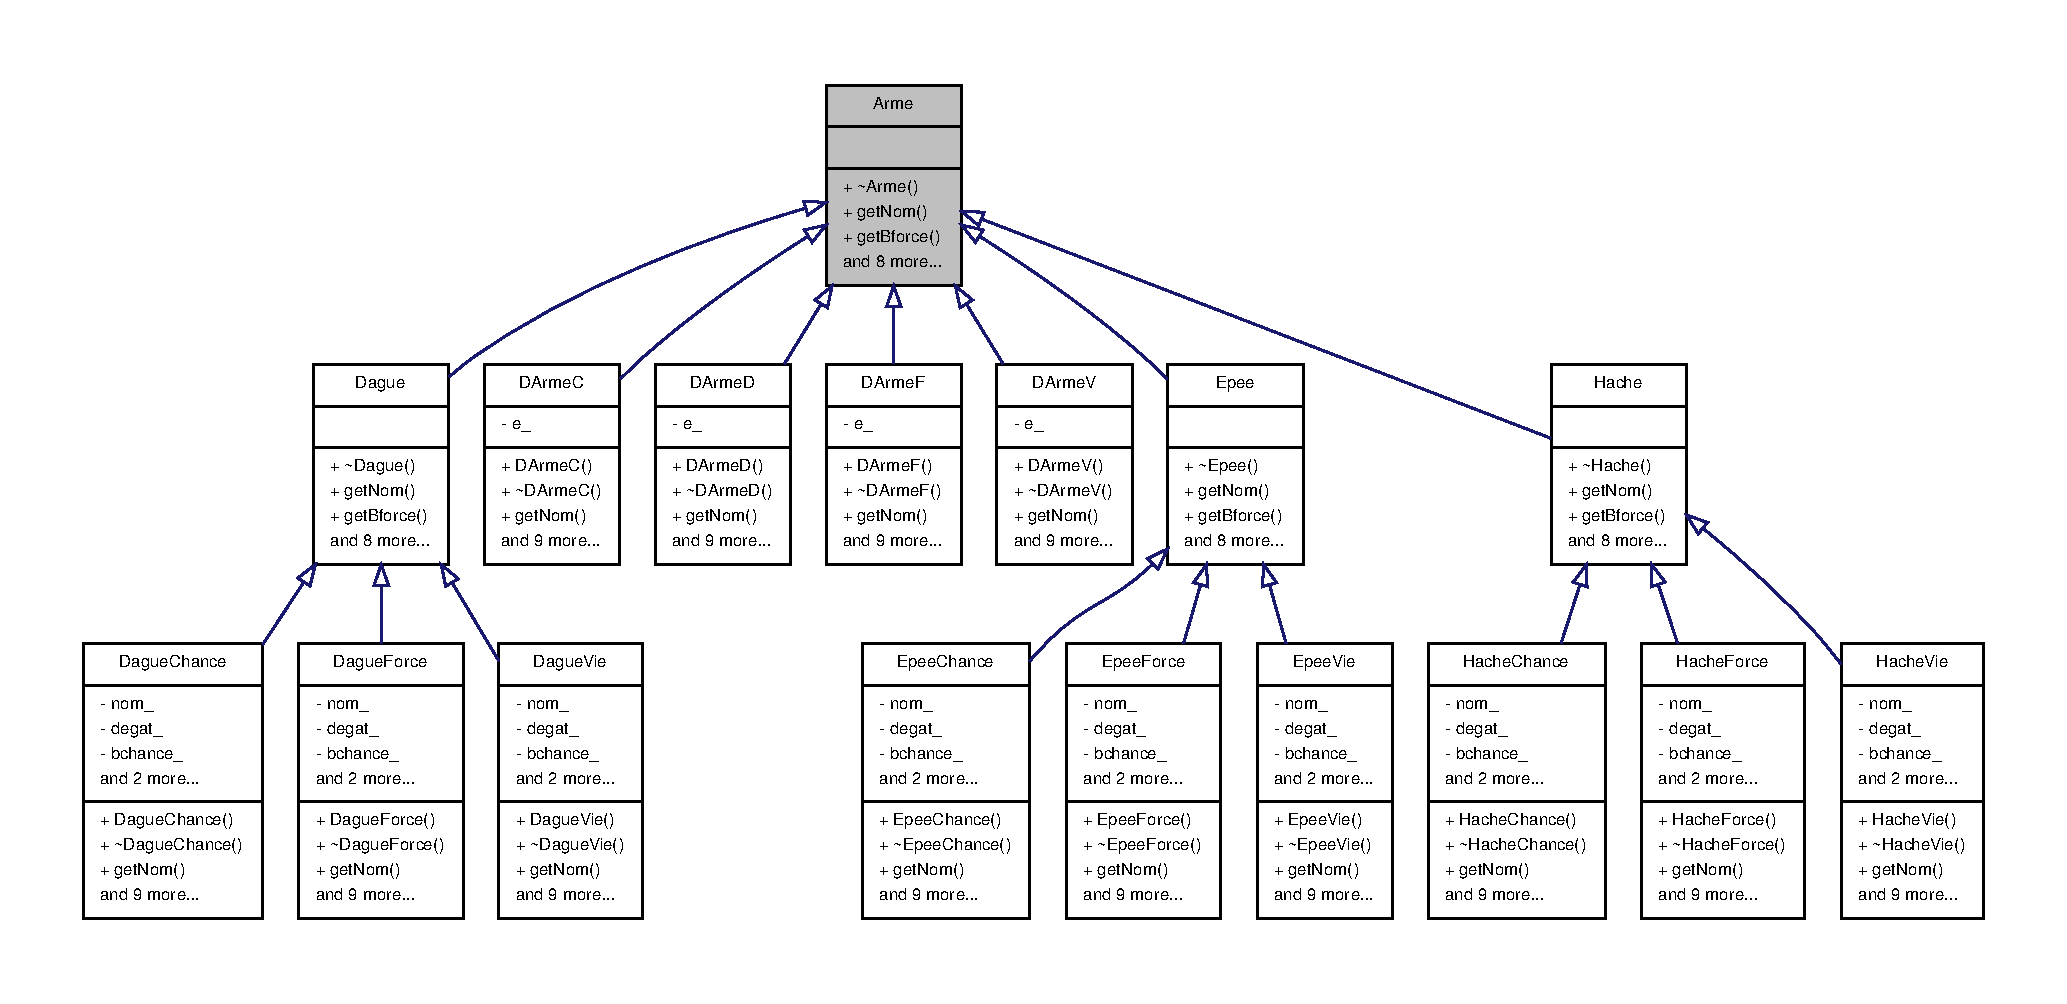
\includegraphics[width=350pt]{class_arme__inherit__graph}
\end{center}
\end{figure}


Graphe de collaboration de Arme\-:\nopagebreak
\begin{figure}[H]
\begin{center}
\leavevmode
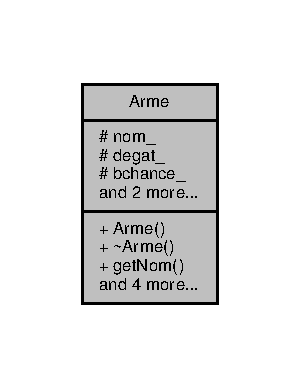
\includegraphics[width=144pt]{class_arme__coll__graph}
\end{center}
\end{figure}
\subsection*{Fonctions membres publiques}
\begin{DoxyCompactItemize}
\item 
virtual {\bf $\sim$\-Arme} ()
\item 
virtual std\-::string {\bf get\-Nom} ()=0
\item 
virtual int {\bf get\-Bforce} ()=0
\item 
virtual int {\bf get\-Bvie} ()=0
\item 
virtual int {\bf get\-Bchance} ()=0
\item 
virtual int {\bf get\-Degat} ()=0
\item 
virtual void {\bf set\-Bforce} (int bforce)=0
\item 
virtual void {\bf set\-Bvie} (int bvie)=0
\item 
virtual void {\bf set\-Bchance} (int bchance)=0
\item 
virtual void {\bf set\-Degat} (int degat)=0
\item 
virtual void {\bf set\-Nom} (std\-::string nom)=0
\end{DoxyCompactItemize}


\subsection{Documentation des constructeurs et destructeur}
\index{Arme@{Arme}!$\sim$\-Arme@{$\sim$\-Arme}}
\index{$\sim$\-Arme@{$\sim$\-Arme}!Arme@{Arme}}
\subsubsection[{$\sim$\-Arme}]{\setlength{\rightskip}{0pt plus 5cm}virtual Arme\-::$\sim$\-Arme (
\begin{DoxyParamCaption}
{}
\end{DoxyParamCaption}
)\hspace{0.3cm}{\ttfamily [inline]}, {\ttfamily [virtual]}}\label{class_arme_acf53bc422814dea9404b34118f243579}


\subsection{Documentation des fonctions membres}
\index{Arme@{Arme}!get\-Bchance@{get\-Bchance}}
\index{get\-Bchance@{get\-Bchance}!Arme@{Arme}}
\subsubsection[{get\-Bchance}]{\setlength{\rightskip}{0pt plus 5cm}virtual int Arme\-::get\-Bchance (
\begin{DoxyParamCaption}
{}
\end{DoxyParamCaption}
)\hspace{0.3cm}{\ttfamily [pure virtual]}}\label{class_arme_afcd4a79f4603cd9ced1eafd15be54316}


Implémenté dans {\bf D\-Arme\-C} \doxyref{}{p.}{class_d_arme_c_a33d7e704e737bdaa81a038dc6753c4c9}, {\bf D\-Arme\-D} \doxyref{}{p.}{class_d_arme_d_aa34e9d9765c2b362667fb98ae48e8e96}, {\bf D\-Arme\-F} \doxyref{}{p.}{class_d_arme_f_a2943f1f73a05531076763dab65dfef47}, {\bf D\-Arme\-V} \doxyref{}{p.}{class_d_arme_v_aa190cd544880030c8bb751e15a352e3f}, {\bf Dague\-Chance} \doxyref{}{p.}{class_dague_chance_ac6146c8ab45cd7d5f8c473f0c5a3f4ef}, {\bf Dague\-Force} \doxyref{}{p.}{class_dague_force_a65da3e61243d0e9f0710385a4b39b858}, {\bf Dague\-Vie} \doxyref{}{p.}{class_dague_vie_ae42dfdf6833cfa9090cd42cbfe17d20c}, {\bf Epee\-Chance} \doxyref{}{p.}{class_epee_chance_a84a21d3d110f35b967a8546c59d66569}, {\bf Epee\-Force} \doxyref{}{p.}{class_epee_force_a6118142e1ffd76560a00d8680794dfdd}, {\bf Epee\-Vie} \doxyref{}{p.}{class_epee_vie_af76e20e49e303804aa8ea2883228089b}, {\bf Hache\-Chance} \doxyref{}{p.}{class_hache_chance_ac7611ecf516fe27a252c6524b28af033}, {\bf Hache\-Force} \doxyref{}{p.}{class_hache_force_a77cd5b2e165e1a551cbfed81abbe4d26}, {\bf Hache\-Vie} \doxyref{}{p.}{class_hache_vie_ae244c830482582a045af8237329b71cb}, {\bf Dague} \doxyref{}{p.}{class_dague_a5de075bd307074a52d7676046ab40ea1}, {\bf Epee} \doxyref{}{p.}{class_epee_ad1fb2f650193d85218f0f9742bac8e26}, et {\bf Hache} \doxyref{}{p.}{class_hache_a2e1cee0ad2fba6b361413412b50126c5}.

\index{Arme@{Arme}!get\-Bforce@{get\-Bforce}}
\index{get\-Bforce@{get\-Bforce}!Arme@{Arme}}
\subsubsection[{get\-Bforce}]{\setlength{\rightskip}{0pt plus 5cm}virtual int Arme\-::get\-Bforce (
\begin{DoxyParamCaption}
{}
\end{DoxyParamCaption}
)\hspace{0.3cm}{\ttfamily [pure virtual]}}\label{class_arme_a25da1859e12ebceb90283fb980f00758}


Implémenté dans {\bf D\-Arme\-C} \doxyref{}{p.}{class_d_arme_c_a8897906b826ed33f3a1af20b7ee7b21c}, {\bf D\-Arme\-D} \doxyref{}{p.}{class_d_arme_d_a501bf8d95f205da038662644c8deb252}, {\bf D\-Arme\-F} \doxyref{}{p.}{class_d_arme_f_a5846b098730320bbcc92d9e9242d0696}, {\bf D\-Arme\-V} \doxyref{}{p.}{class_d_arme_v_a70323fba012f9cc56eff0c45ccdc98bb}, {\bf Dague\-Chance} \doxyref{}{p.}{class_dague_chance_ad5a65eb71a84fc9d9d081e94b6d88257}, {\bf Dague\-Force} \doxyref{}{p.}{class_dague_force_a5d8a8017647abdd63eb3bb4c0e87500f}, {\bf Dague\-Vie} \doxyref{}{p.}{class_dague_vie_aab12c82cde51d11d83a465d9d076349f}, {\bf Epee\-Chance} \doxyref{}{p.}{class_epee_chance_ad2f48aaa05c975890985eaffd22027bd}, {\bf Epee\-Force} \doxyref{}{p.}{class_epee_force_a9c38c3126806fb0358044b73736c8ac5}, {\bf Epee\-Vie} \doxyref{}{p.}{class_epee_vie_a848e8f74dfb7b4aa13b23cb1174964d7}, {\bf Hache\-Chance} \doxyref{}{p.}{class_hache_chance_ac4746ffe9c6e0c4195b72d44f488bbc2}, {\bf Hache\-Force} \doxyref{}{p.}{class_hache_force_a22709000dd15b23f13318849ca560e96}, {\bf Hache\-Vie} \doxyref{}{p.}{class_hache_vie_a35e7a9726762430e42d3a51fbf948445}, {\bf Dague} \doxyref{}{p.}{class_dague_af9baa3478d3800f285bb961a73fb061f}, {\bf Epee} \doxyref{}{p.}{class_epee_a1e4ac064617efa372aa48e122da62da5}, et {\bf Hache} \doxyref{}{p.}{class_hache_a3ca034bcd0975a0163778b19f713d11f}.

\index{Arme@{Arme}!get\-Bvie@{get\-Bvie}}
\index{get\-Bvie@{get\-Bvie}!Arme@{Arme}}
\subsubsection[{get\-Bvie}]{\setlength{\rightskip}{0pt plus 5cm}virtual int Arme\-::get\-Bvie (
\begin{DoxyParamCaption}
{}
\end{DoxyParamCaption}
)\hspace{0.3cm}{\ttfamily [pure virtual]}}\label{class_arme_ad07794203a8fa685391cd6c107529aa1}


Implémenté dans {\bf D\-Arme\-C} \doxyref{}{p.}{class_d_arme_c_aac29897179bf6d6b3d98b68333097736}, {\bf D\-Arme\-D} \doxyref{}{p.}{class_d_arme_d_a979a3cf9fbf2c59fd38ad1ce81d2fc06}, {\bf D\-Arme\-F} \doxyref{}{p.}{class_d_arme_f_aeee4b538f13d9d7336eb75700a7ca6e0}, {\bf D\-Arme\-V} \doxyref{}{p.}{class_d_arme_v_afcde018608ec17457b68c794ef686640}, {\bf Dague\-Chance} \doxyref{}{p.}{class_dague_chance_a07dfcc6377639fdfe6a0ee6c4a8b3729}, {\bf Dague\-Force} \doxyref{}{p.}{class_dague_force_a15abc56ba8ea78cc3ed476af5b8820a0}, {\bf Dague\-Vie} \doxyref{}{p.}{class_dague_vie_a751a65bab6845a4e1cf706e2d575ae23}, {\bf Epee\-Chance} \doxyref{}{p.}{class_epee_chance_af422c51427e9fefc10c597ffb2ab23ae}, {\bf Epee\-Force} \doxyref{}{p.}{class_epee_force_a789be79cffe9a45a7be3bf01c66301db}, {\bf Epee\-Vie} \doxyref{}{p.}{class_epee_vie_af3694dc84eff46350825f7e4955afa90}, {\bf Hache\-Chance} \doxyref{}{p.}{class_hache_chance_a88c48462f592dff1a1d077170738176c}, {\bf Hache\-Force} \doxyref{}{p.}{class_hache_force_a2f820c9c3b98cd37020a0d0bf07df4d4}, {\bf Hache\-Vie} \doxyref{}{p.}{class_hache_vie_adccb20b8695c3b7d57a0ffcba96e1fc3}, {\bf Dague} \doxyref{}{p.}{class_dague_a35d0387f7d2249e7369b89f09427d36b}, {\bf Epee} \doxyref{}{p.}{class_epee_ae3e836b6821474eaa93653148404fb72}, et {\bf Hache} \doxyref{}{p.}{class_hache_aef2b82ff40e40047bb6b1571dde7c456}.

\index{Arme@{Arme}!get\-Degat@{get\-Degat}}
\index{get\-Degat@{get\-Degat}!Arme@{Arme}}
\subsubsection[{get\-Degat}]{\setlength{\rightskip}{0pt plus 5cm}virtual int Arme\-::get\-Degat (
\begin{DoxyParamCaption}
{}
\end{DoxyParamCaption}
)\hspace{0.3cm}{\ttfamily [pure virtual]}}\label{class_arme_a93e1b6f8c800359c7651b2fc456a3ee1}


Implémenté dans {\bf D\-Arme\-C} \doxyref{}{p.}{class_d_arme_c_a3819d78ab37fd6fae45bb03eb15fc03a}, {\bf D\-Arme\-D} \doxyref{}{p.}{class_d_arme_d_a027754e8974e05fac348cdbd88c2b1a7}, {\bf D\-Arme\-F} \doxyref{}{p.}{class_d_arme_f_a43f33d4229200d1eed5bfaa577c994c2}, {\bf D\-Arme\-V} \doxyref{}{p.}{class_d_arme_v_afda7872bb1ba6eb8b988c12524faa211}, {\bf Dague\-Chance} \doxyref{}{p.}{class_dague_chance_acfff9ba3d01879aa998c4eb75724bec4}, {\bf Dague\-Force} \doxyref{}{p.}{class_dague_force_adb3447fe7c3670566a032f476334c1d5}, {\bf Dague\-Vie} \doxyref{}{p.}{class_dague_vie_a5290ff3924ec192fbdc9b763d329bb39}, {\bf Epee\-Chance} \doxyref{}{p.}{class_epee_chance_a506a2b47b5f00e862db1ccd2e87dd9be}, {\bf Epee\-Force} \doxyref{}{p.}{class_epee_force_aa3fc41a797c108bbdb85b6a72c595aac}, {\bf Epee\-Vie} \doxyref{}{p.}{class_epee_vie_aede2704c0cb5f4339e6d14f0f4267d36}, {\bf Hache\-Chance} \doxyref{}{p.}{class_hache_chance_a000478fd8ab08509e69eeafa9594b132}, {\bf Hache\-Force} \doxyref{}{p.}{class_hache_force_a37362152a01b049d983587644704fb63}, {\bf Hache\-Vie} \doxyref{}{p.}{class_hache_vie_a148acd3cb39ae49c1d60150253c25211}, {\bf Dague} \doxyref{}{p.}{class_dague_a25298dd54ed21b88ff1694962711028f}, {\bf Epee} \doxyref{}{p.}{class_epee_a389f6107671a22f69cca040d63aef647}, et {\bf Hache} \doxyref{}{p.}{class_hache_a2ffc6914be4b1a61d65bcb9469b8625f}.

\index{Arme@{Arme}!get\-Nom@{get\-Nom}}
\index{get\-Nom@{get\-Nom}!Arme@{Arme}}
\subsubsection[{get\-Nom}]{\setlength{\rightskip}{0pt plus 5cm}virtual std\-::string Arme\-::get\-Nom (
\begin{DoxyParamCaption}
{}
\end{DoxyParamCaption}
)\hspace{0.3cm}{\ttfamily [pure virtual]}}\label{class_arme_a0b6a30975be57770c6cae357b52395a0}


Implémenté dans {\bf D\-Arme\-C} \doxyref{}{p.}{class_d_arme_c_ac7553787a322cc23a8d1500b1e12f3cd}, {\bf D\-Arme\-D} \doxyref{}{p.}{class_d_arme_d_aed705127e47b1122eb66a93fe414d4e6}, {\bf D\-Arme\-F} \doxyref{}{p.}{class_d_arme_f_ad780ace9451a25b7eafb84d9d4f5a009}, {\bf D\-Arme\-V} \doxyref{}{p.}{class_d_arme_v_ab3b60176e59c3cd04583a584ab02ef78}, {\bf Dague\-Chance} \doxyref{}{p.}{class_dague_chance_a955ed40b9c57d721de4e4994ff47ed9d}, {\bf Dague\-Force} \doxyref{}{p.}{class_dague_force_aaee0493fa04f2633edb9d383a5997243}, {\bf Dague\-Vie} \doxyref{}{p.}{class_dague_vie_a42d8393844d6f9d81759624be1a4edbc}, {\bf Epee\-Chance} \doxyref{}{p.}{class_epee_chance_a730b12fbd3ca6cc8824343bf02319285}, {\bf Epee\-Force} \doxyref{}{p.}{class_epee_force_a6fe11e6946366b792b6547e3e3427c1d}, {\bf Epee\-Vie} \doxyref{}{p.}{class_epee_vie_a850643675b0b126aeedcf33d75fcd9e8}, {\bf Hache\-Chance} \doxyref{}{p.}{class_hache_chance_a7b79ab8133ce1c7b7061f721c94c29c7}, {\bf Hache\-Force} \doxyref{}{p.}{class_hache_force_a0ca86fcace6718e4ab265b379c3521e6}, {\bf Hache\-Vie} \doxyref{}{p.}{class_hache_vie_a847298f6146d51b196c2bcb80a11429d}, {\bf Dague} \doxyref{}{p.}{class_dague_a4ac0c92d71164c8a9e54e626602d49ac}, {\bf Epee} \doxyref{}{p.}{class_epee_a3a006ae3e7e9f3275100a76f572dc085}, et {\bf Hache} \doxyref{}{p.}{class_hache_a8306bd1a3a278e68cdb12081551451e1}.

\index{Arme@{Arme}!set\-Bchance@{set\-Bchance}}
\index{set\-Bchance@{set\-Bchance}!Arme@{Arme}}
\subsubsection[{set\-Bchance}]{\setlength{\rightskip}{0pt plus 5cm}virtual void Arme\-::set\-Bchance (
\begin{DoxyParamCaption}
\item[{int}]{bchance}
\end{DoxyParamCaption}
)\hspace{0.3cm}{\ttfamily [pure virtual]}}\label{class_arme_a27aa7d294d01ea38975841ea680a815a}


Implémenté dans {\bf D\-Arme\-C} \doxyref{}{p.}{class_d_arme_c_a636d1d22f4769fc1a6f89125dd58f5c9}, {\bf D\-Arme\-D} \doxyref{}{p.}{class_d_arme_d_a8aceb11c1cb459516442d6437f139304}, {\bf D\-Arme\-F} \doxyref{}{p.}{class_d_arme_f_a65777071151d6c367fa58410b941effb}, {\bf D\-Arme\-V} \doxyref{}{p.}{class_d_arme_v_ada8a7f4bd1b02648dd4ad1efa9022720}, {\bf Dague\-Chance} \doxyref{}{p.}{class_dague_chance_a492f6549765cb10511d4dd7213036995}, {\bf Dague\-Force} \doxyref{}{p.}{class_dague_force_a291dc10a8c54d528b8ef2391963ee29f}, {\bf Dague\-Vie} \doxyref{}{p.}{class_dague_vie_a6a78fd29aecba8f468106dc434c68648}, {\bf Epee\-Chance} \doxyref{}{p.}{class_epee_chance_a1a5f6547d4bead671c2841a2dbec771e}, {\bf Epee\-Force} \doxyref{}{p.}{class_epee_force_a079f803779bd26e5baae1330c50fa91f}, {\bf Epee\-Vie} \doxyref{}{p.}{class_epee_vie_abb56e1ae6ee02d815e56ad9ea68bd082}, {\bf Hache\-Chance} \doxyref{}{p.}{class_hache_chance_ac3901bd8f4cbb546e1ef88344790b5a0}, {\bf Hache\-Force} \doxyref{}{p.}{class_hache_force_af11b69b98aa5e58e8f4861ef330a352b}, {\bf Hache\-Vie} \doxyref{}{p.}{class_hache_vie_aa1e657df5b81cdcaf0a90d82b38190d6}, {\bf Dague} \doxyref{}{p.}{class_dague_ae58691c16eebd09f03aac47c3b70d869}, {\bf Epee} \doxyref{}{p.}{class_epee_ac88031cb62f0c374ae0873ccd99d91bf}, et {\bf Hache} \doxyref{}{p.}{class_hache_af7d3053935ff6dc5d6dd8b4dfacbed02}.

\index{Arme@{Arme}!set\-Bforce@{set\-Bforce}}
\index{set\-Bforce@{set\-Bforce}!Arme@{Arme}}
\subsubsection[{set\-Bforce}]{\setlength{\rightskip}{0pt plus 5cm}virtual void Arme\-::set\-Bforce (
\begin{DoxyParamCaption}
\item[{int}]{bforce}
\end{DoxyParamCaption}
)\hspace{0.3cm}{\ttfamily [pure virtual]}}\label{class_arme_a8806ba4300d435ebe71bb4b9829296e8}


Implémenté dans {\bf D\-Arme\-C} \doxyref{}{p.}{class_d_arme_c_a9ce567806ba4e74c55753cfb1080a08d}, {\bf D\-Arme\-D} \doxyref{}{p.}{class_d_arme_d_af534b933752424773b55c198f60c17e4}, {\bf D\-Arme\-F} \doxyref{}{p.}{class_d_arme_f_a26e62c08650fc3ac3ee4827a1deacbe7}, {\bf D\-Arme\-V} \doxyref{}{p.}{class_d_arme_v_a29634cf4d2658adc00cc5ebf52262c47}, {\bf Dague\-Chance} \doxyref{}{p.}{class_dague_chance_ac2fd0b9d309ba0c335305ecdf57fa56b}, {\bf Dague\-Force} \doxyref{}{p.}{class_dague_force_aac379e382d25e38bf77b91e3c3ab2424}, {\bf Dague\-Vie} \doxyref{}{p.}{class_dague_vie_a3fcf25af8aabbdea4a11a9386a020c9d}, {\bf Epee\-Chance} \doxyref{}{p.}{class_epee_chance_a26213bb7fee03bd5e2450aaa31970bfd}, {\bf Epee\-Force} \doxyref{}{p.}{class_epee_force_add1829b57101aa105503fbde51b84c99}, {\bf Epee\-Vie} \doxyref{}{p.}{class_epee_vie_aaff428a4663555db0520e3528c8964d5}, {\bf Hache\-Chance} \doxyref{}{p.}{class_hache_chance_a3288d918235168d56c5827a44beca8cd}, {\bf Hache\-Force} \doxyref{}{p.}{class_hache_force_a2a3749b6222565dd46fb5e2241fa39b1}, {\bf Hache\-Vie} \doxyref{}{p.}{class_hache_vie_aa14e47e7518d2b05f4ce65c67b06e3b4}, {\bf Dague} \doxyref{}{p.}{class_dague_aff6198d6598ae0e1e142aed959d1a150}, {\bf Epee} \doxyref{}{p.}{class_epee_a98bc94805ee7d9d64a4e2f775bedb9d7}, et {\bf Hache} \doxyref{}{p.}{class_hache_a807cb1478fad141514cb218b05679da6}.

\index{Arme@{Arme}!set\-Bvie@{set\-Bvie}}
\index{set\-Bvie@{set\-Bvie}!Arme@{Arme}}
\subsubsection[{set\-Bvie}]{\setlength{\rightskip}{0pt plus 5cm}virtual void Arme\-::set\-Bvie (
\begin{DoxyParamCaption}
\item[{int}]{bvie}
\end{DoxyParamCaption}
)\hspace{0.3cm}{\ttfamily [pure virtual]}}\label{class_arme_a0580ea53e4254942a4ef82aec8706ead}


Implémenté dans {\bf D\-Arme\-C} \doxyref{}{p.}{class_d_arme_c_a758cea41196bcb19552d72955ec04735}, {\bf D\-Arme\-D} \doxyref{}{p.}{class_d_arme_d_a25f28d3f69c6bb7372cfe4fe686ec467}, {\bf D\-Arme\-F} \doxyref{}{p.}{class_d_arme_f_a65c716090661cd7b7682b45a367edb2f}, {\bf D\-Arme\-V} \doxyref{}{p.}{class_d_arme_v_a855b84902ad793574ded99f5067f7e57}, {\bf Dague\-Chance} \doxyref{}{p.}{class_dague_chance_a3cc292f96dc5a7f2f2b9c313e1909f2e}, {\bf Dague\-Force} \doxyref{}{p.}{class_dague_force_a9cd47a8d709119faa983f40e986afa1f}, {\bf Dague\-Vie} \doxyref{}{p.}{class_dague_vie_ac172f87953d202cc839acb687ba8f504}, {\bf Epee\-Chance} \doxyref{}{p.}{class_epee_chance_a8cc304a06901a87fef0441258362b919}, {\bf Epee\-Force} \doxyref{}{p.}{class_epee_force_ac46b84be9efab7a8c9c6527abc325e89}, {\bf Epee\-Vie} \doxyref{}{p.}{class_epee_vie_a0f8f49a705cc0b8be0417e2aba4bdf11}, {\bf Hache\-Chance} \doxyref{}{p.}{class_hache_chance_af0a35f092e239683e6af392d85684e3a}, {\bf Hache\-Force} \doxyref{}{p.}{class_hache_force_a6dcc31dd61adcbea38a5a7fb884a82a9}, {\bf Hache\-Vie} \doxyref{}{p.}{class_hache_vie_a933eeb35c6313efa373a26a00d348614}, {\bf Dague} \doxyref{}{p.}{class_dague_adb4c176caf63fb57a4012c104f0bf35b}, {\bf Epee} \doxyref{}{p.}{class_epee_a643a5177f1f211c080c546430c1c4967}, et {\bf Hache} \doxyref{}{p.}{class_hache_a5b9ff524f1ff49ef11c2f5c031ee5151}.

\index{Arme@{Arme}!set\-Degat@{set\-Degat}}
\index{set\-Degat@{set\-Degat}!Arme@{Arme}}
\subsubsection[{set\-Degat}]{\setlength{\rightskip}{0pt plus 5cm}virtual void Arme\-::set\-Degat (
\begin{DoxyParamCaption}
\item[{int}]{degat}
\end{DoxyParamCaption}
)\hspace{0.3cm}{\ttfamily [pure virtual]}}\label{class_arme_a2e2cd008885e4ba4dca346905e7e5f73}


Implémenté dans {\bf D\-Arme\-C} \doxyref{}{p.}{class_d_arme_c_a80521baa4e17c25587c5131be58a6f7a}, {\bf D\-Arme\-D} \doxyref{}{p.}{class_d_arme_d_aa31a6bde42462f4ffc84f73e737dfdf0}, {\bf D\-Arme\-F} \doxyref{}{p.}{class_d_arme_f_a6de6a02ec98b81d18d0d1b23c3d816c6}, {\bf D\-Arme\-V} \doxyref{}{p.}{class_d_arme_v_ae3df741a51c1c2a7993f95b69adcb9ff}, {\bf Dague\-Chance} \doxyref{}{p.}{class_dague_chance_a61b3084db9375853a1f60e99ad584afe}, {\bf Dague\-Force} \doxyref{}{p.}{class_dague_force_a3b4d211b9f6c67ab7cfb76051b143dea}, {\bf Dague\-Vie} \doxyref{}{p.}{class_dague_vie_adab4e95d5f1b30ac3a43c5832f67c942}, {\bf Epee\-Chance} \doxyref{}{p.}{class_epee_chance_a269f1a4f174d4d95a53f316bbda19b27}, {\bf Epee\-Force} \doxyref{}{p.}{class_epee_force_a443d616be62b986ad26172b42354c577}, {\bf Epee\-Vie} \doxyref{}{p.}{class_epee_vie_a0a0ddd9571b2f9ea9c837b082d0bb680}, {\bf Hache\-Chance} \doxyref{}{p.}{class_hache_chance_a6f891d08c12acc2f5ac28e16d73e4f76}, {\bf Hache\-Force} \doxyref{}{p.}{class_hache_force_a31776c8f6e1fb28773922b85a3191f10}, {\bf Hache\-Vie} \doxyref{}{p.}{class_hache_vie_a1eb5f62f8214e718f367d0e3bc38b261}, {\bf Dague} \doxyref{}{p.}{class_dague_a14c7a619bb8c4dfd54c3b198b303821d}, {\bf Epee} \doxyref{}{p.}{class_epee_a35ed08f9927b855b5b09643d00297dbc}, et {\bf Hache} \doxyref{}{p.}{class_hache_ac655e84171b801a16975ed443284b6f5}.

\index{Arme@{Arme}!set\-Nom@{set\-Nom}}
\index{set\-Nom@{set\-Nom}!Arme@{Arme}}
\subsubsection[{set\-Nom}]{\setlength{\rightskip}{0pt plus 5cm}virtual void Arme\-::set\-Nom (
\begin{DoxyParamCaption}
\item[{std\-::string}]{nom}
\end{DoxyParamCaption}
)\hspace{0.3cm}{\ttfamily [pure virtual]}}\label{class_arme_a561f12b90bd01d26328541ba54f6aaa6}


Implémenté dans {\bf D\-Arme\-C} \doxyref{}{p.}{class_d_arme_c_aad343bffc110d37e041d0bfc00f632a0}, {\bf D\-Arme\-D} \doxyref{}{p.}{class_d_arme_d_acadea2841f93506a778dd42141e09b9f}, {\bf D\-Arme\-F} \doxyref{}{p.}{class_d_arme_f_a55d6f314fc9095bb92a60e0e686d9a43}, {\bf D\-Arme\-V} \doxyref{}{p.}{class_d_arme_v_a4779d99027ae0e7ea5f9e4a7c85f6859}, {\bf Dague\-Chance} \doxyref{}{p.}{class_dague_chance_a79bcbf32965ad2a43b32c86fc630d60f}, {\bf Dague\-Force} \doxyref{}{p.}{class_dague_force_ac5a74a106d950a5e0ae77a083dd4c235}, {\bf Dague\-Vie} \doxyref{}{p.}{class_dague_vie_ad99195a86efd066f81b46c44a645696f}, {\bf Epee\-Chance} \doxyref{}{p.}{class_epee_chance_a7095d5eff815de7813ebb621d35f453b}, {\bf Epee\-Force} \doxyref{}{p.}{class_epee_force_a50e44b3fb4d0ecd607342fa2a5ddb600}, {\bf Epee\-Vie} \doxyref{}{p.}{class_epee_vie_a32ca3accce018500c19a225e34eea7f8}, {\bf Hache\-Chance} \doxyref{}{p.}{class_hache_chance_a97adf98356bd3eb9e156ff7101ed69d1}, {\bf Hache\-Force} \doxyref{}{p.}{class_hache_force_a9680f2f7985a59cafda40de2a4d15ee2}, {\bf Hache\-Vie} \doxyref{}{p.}{class_hache_vie_aba2dd35bcda9c87ded61a887e5e42658}, {\bf Dague} \doxyref{}{p.}{class_dague_a5b5f19a4e51c2fb13cbf320044e87697}, {\bf Epee} \doxyref{}{p.}{class_epee_a974abf77e22496b7d54f2357fbd664a2}, et {\bf Hache} \doxyref{}{p.}{class_hache_ad1904c7b0200c185225901342146f99b}.



La documentation de cette classe a été générée à partir du fichier suivant \-:\begin{DoxyCompactItemize}
\item 
src/{\bf Arme.\-hpp}\end{DoxyCompactItemize}

\hypertarget{class_casque}{\section{Référence de la classe Casque}
\label{class_casque}\index{Casque@{Casque}}
}


\hyperlink{class_casque}{Casque} herite de \hyperlink{class_equipement}{Equipement}.  




Graphe d'héritage de Casque\-:
\nopagebreak
\begin{figure}[H]
\begin{center}
\leavevmode
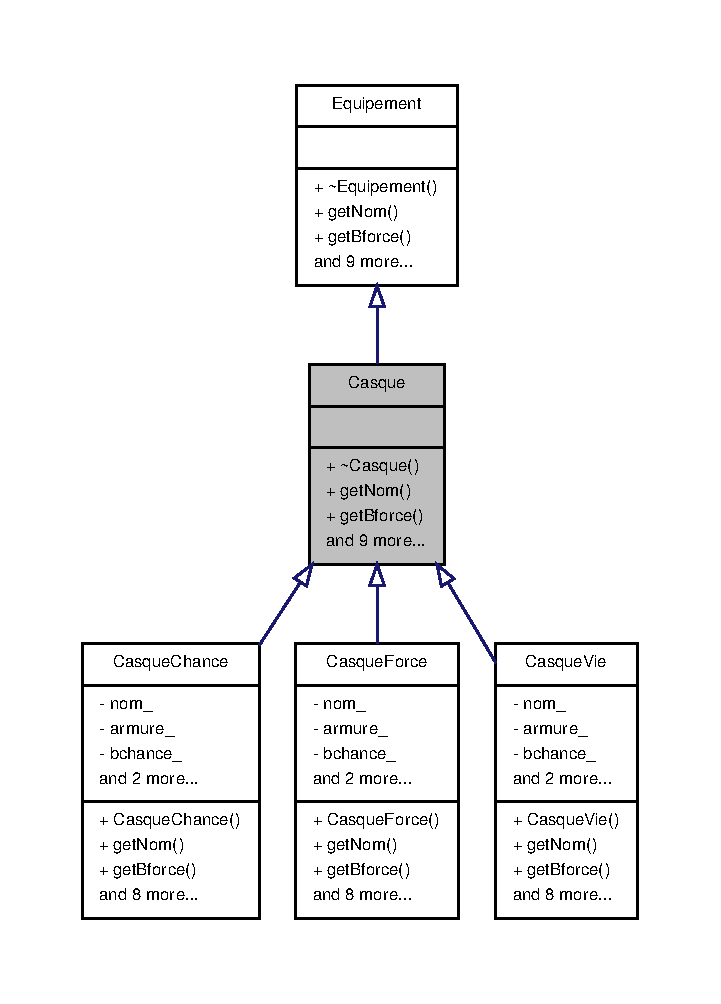
\includegraphics[width=346pt]{class_casque__inherit__graph}
\end{center}
\end{figure}


Graphe de collaboration de Casque\-:
\nopagebreak
\begin{figure}[H]
\begin{center}
\leavevmode
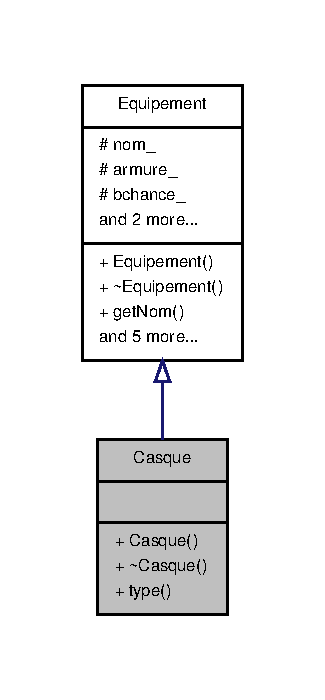
\includegraphics[width=156pt]{class_casque__coll__graph}
\end{center}
\end{figure}
\subsection*{Fonctions membres publiques}
\begin{DoxyCompactItemize}
\item 
int \hyperlink{class_casque_acb93c4c89d61c945d75ee3d47bede861}{type} ()
\begin{DoxyCompactList}\small\item\em Renvoie le type de l'equipement. \end{DoxyCompactList}\item 
virtual std\-::string \hyperlink{class_equipement_a0b0426a70bfce6e7c3efac605b75cd8e}{get\-Nom} ()
\begin{DoxyCompactList}\small\item\em Retourne le nom de l'equipement. \end{DoxyCompactList}\item 
virtual int \hyperlink{class_equipement_aabcf10fd762945fa4a37a9cf8321f463}{get\-Bforce} ()
\begin{DoxyCompactList}\small\item\em Retourne le bonus de force. \end{DoxyCompactList}\item 
virtual int \hyperlink{class_equipement_ad9fd7528c4f181970b7a0877f4145f89}{get\-Bvie} ()
\begin{DoxyCompactList}\small\item\em Retourne le bonus de vie. \end{DoxyCompactList}\item 
virtual int \hyperlink{class_equipement_a73485135eacdf30d5f49c9e34e5f4d0e}{get\-Bchance} ()
\begin{DoxyCompactList}\small\item\em Retourne le bonus de chance. \end{DoxyCompactList}\item 
virtual int \hyperlink{class_equipement_a8577d49fd00b8effa39388feccb29901}{get\-Armure} ()
\begin{DoxyCompactList}\small\item\em Retourne l'armure fournie par l'equipement. \end{DoxyCompactList}\end{DoxyCompactItemize}
\subsection*{Attributs protégés}
\begin{DoxyCompactItemize}
\item 
\hypertarget{class_equipement_a930290aac01ecd40c7a646ab8f66d742}{std\-::string {\bfseries nom\-\_\-}}\label{class_equipement_a930290aac01ecd40c7a646ab8f66d742}

\item 
\hypertarget{class_equipement_a69339ce4f1f5fe7e6fcdeda5b74c14a4}{int {\bfseries armure\-\_\-}}\label{class_equipement_a69339ce4f1f5fe7e6fcdeda5b74c14a4}

\item 
\hypertarget{class_equipement_aa70effa6a8144fe1f4fe874af7139793}{int {\bfseries bchance\-\_\-}}\label{class_equipement_aa70effa6a8144fe1f4fe874af7139793}

\item 
\hypertarget{class_equipement_a73ac5bff40e3f6bf1d8e6f0e524e750f}{int {\bfseries bvie\-\_\-}}\label{class_equipement_a73ac5bff40e3f6bf1d8e6f0e524e750f}

\item 
\hypertarget{class_equipement_af87cf3f291386d5401be6994dd8fb8be}{int {\bfseries bforce\-\_\-}}\label{class_equipement_af87cf3f291386d5401be6994dd8fb8be}

\end{DoxyCompactItemize}


\subsection{Description détaillée}
\hyperlink{class_casque}{Casque} herite de \hyperlink{class_equipement}{Equipement}. 

\subsection{Documentation des fonctions membres}
\hypertarget{class_equipement_a8577d49fd00b8effa39388feccb29901}{\index{Casque@{Casque}!get\-Armure@{get\-Armure}}
\index{get\-Armure@{get\-Armure}!Casque@{Casque}}
\subsubsection[{get\-Armure}]{\setlength{\rightskip}{0pt plus 5cm}int Equipement\-::get\-Armure (
\begin{DoxyParamCaption}
{}
\end{DoxyParamCaption}
)\hspace{0.3cm}{\ttfamily [virtual]}, {\ttfamily [inherited]}}}\label{class_equipement_a8577d49fd00b8effa39388feccb29901}


Retourne l'armure fournie par l'equipement. 

\begin{DoxyReturn}{Renvoie}
armure 
\end{DoxyReturn}


Réimplémentée dans \hyperlink{class_d_equip_a7b2c8227ae884c23ccc8f3a2e5702186}{D\-Equip}.

\hypertarget{class_equipement_a73485135eacdf30d5f49c9e34e5f4d0e}{\index{Casque@{Casque}!get\-Bchance@{get\-Bchance}}
\index{get\-Bchance@{get\-Bchance}!Casque@{Casque}}
\subsubsection[{get\-Bchance}]{\setlength{\rightskip}{0pt plus 5cm}int Equipement\-::get\-Bchance (
\begin{DoxyParamCaption}
{}
\end{DoxyParamCaption}
)\hspace{0.3cm}{\ttfamily [virtual]}, {\ttfamily [inherited]}}}\label{class_equipement_a73485135eacdf30d5f49c9e34e5f4d0e}


Retourne le bonus de chance. 

\begin{DoxyReturn}{Renvoie}
Bchance 
\end{DoxyReturn}


Réimplémentée dans \hyperlink{class_d_equip_a39407c92f0de87306a33f57fd22ce997}{D\-Equip}.

\hypertarget{class_equipement_aabcf10fd762945fa4a37a9cf8321f463}{\index{Casque@{Casque}!get\-Bforce@{get\-Bforce}}
\index{get\-Bforce@{get\-Bforce}!Casque@{Casque}}
\subsubsection[{get\-Bforce}]{\setlength{\rightskip}{0pt plus 5cm}int Equipement\-::get\-Bforce (
\begin{DoxyParamCaption}
{}
\end{DoxyParamCaption}
)\hspace{0.3cm}{\ttfamily [virtual]}, {\ttfamily [inherited]}}}\label{class_equipement_aabcf10fd762945fa4a37a9cf8321f463}


Retourne le bonus de force. 

\begin{DoxyReturn}{Renvoie}
Bforce 
\end{DoxyReturn}


Réimplémentée dans \hyperlink{class_d_equip_adb6645ce01c12a4cb3fe0b522ea6b25e}{D\-Equip}.

\hypertarget{class_equipement_ad9fd7528c4f181970b7a0877f4145f89}{\index{Casque@{Casque}!get\-Bvie@{get\-Bvie}}
\index{get\-Bvie@{get\-Bvie}!Casque@{Casque}}
\subsubsection[{get\-Bvie}]{\setlength{\rightskip}{0pt plus 5cm}int Equipement\-::get\-Bvie (
\begin{DoxyParamCaption}
{}
\end{DoxyParamCaption}
)\hspace{0.3cm}{\ttfamily [virtual]}, {\ttfamily [inherited]}}}\label{class_equipement_ad9fd7528c4f181970b7a0877f4145f89}


Retourne le bonus de vie. 

\begin{DoxyReturn}{Renvoie}
Bvie 
\end{DoxyReturn}


Réimplémentée dans \hyperlink{class_d_equip_a085ea4ac21c238d8c147ff4e6d74794f}{D\-Equip}.

\hypertarget{class_equipement_a0b0426a70bfce6e7c3efac605b75cd8e}{\index{Casque@{Casque}!get\-Nom@{get\-Nom}}
\index{get\-Nom@{get\-Nom}!Casque@{Casque}}
\subsubsection[{get\-Nom}]{\setlength{\rightskip}{0pt plus 5cm}std\-::string Equipement\-::get\-Nom (
\begin{DoxyParamCaption}
{}
\end{DoxyParamCaption}
)\hspace{0.3cm}{\ttfamily [virtual]}, {\ttfamily [inherited]}}}\label{class_equipement_a0b0426a70bfce6e7c3efac605b75cd8e}


Retourne le nom de l'equipement. 

\begin{DoxyReturn}{Renvoie}
Nom 
\end{DoxyReturn}
\hypertarget{class_casque_acb93c4c89d61c945d75ee3d47bede861}{\index{Casque@{Casque}!type@{type}}
\index{type@{type}!Casque@{Casque}}
\subsubsection[{type}]{\setlength{\rightskip}{0pt plus 5cm}int Casque\-::type (
\begin{DoxyParamCaption}
{}
\end{DoxyParamCaption}
)\hspace{0.3cm}{\ttfamily [virtual]}}}\label{class_casque_acb93c4c89d61c945d75ee3d47bede861}


Renvoie le type de l'equipement. 

\begin{DoxyReturn}{Renvoie}
int 
\end{DoxyReturn}


Implémente \hyperlink{class_equipement_a05b2c9d4cf22b6aefb6603fa4e322aa2}{Equipement}.


\section{Référence de la classe Casque\-Chance}
\label{class_casque_chance}\index{Casque\-Chance@{Casque\-Chance}}


Graphe d'héritage de Casque\-Chance\-:\nopagebreak
\begin{figure}[H]
\begin{center}
\leavevmode
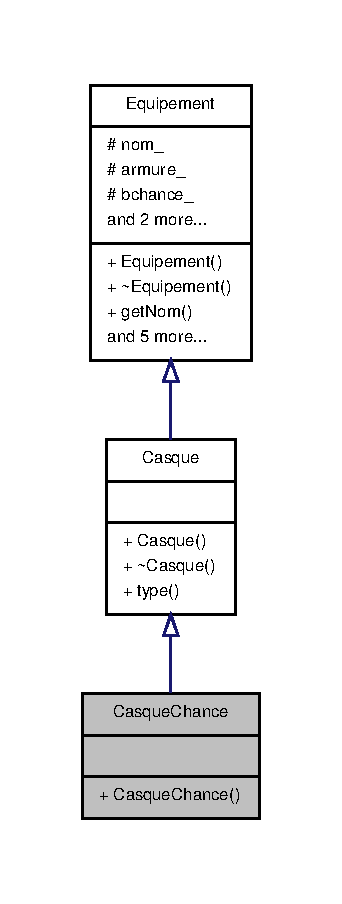
\includegraphics[width=164pt]{class_casque_chance__inherit__graph}
\end{center}
\end{figure}


Graphe de collaboration de Casque\-Chance\-:\nopagebreak
\begin{figure}[H]
\begin{center}
\leavevmode
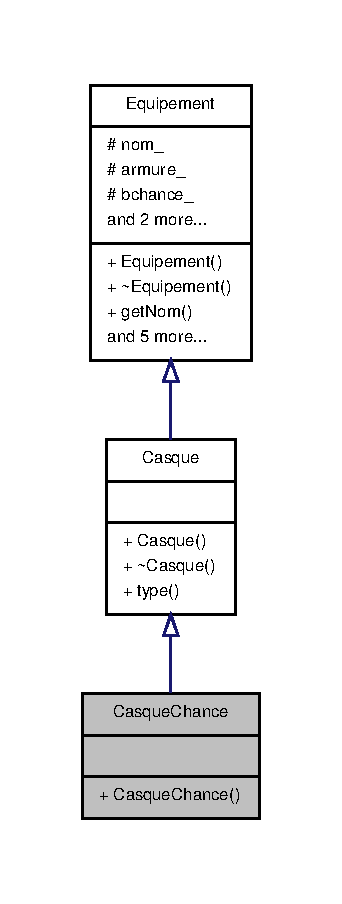
\includegraphics[width=164pt]{class_casque_chance__coll__graph}
\end{center}
\end{figure}
\subsection*{Fonctions membres publiques}
\begin{DoxyCompactItemize}
\item 
{\bf Casque\-Chance} ()
\item 
std\-::string {\bf get\-Nom} ()
\item 
int {\bf get\-Bforce} ()
\item 
int {\bf get\-Bvie} ()
\item 
int {\bf get\-Bchance} ()
\item 
int {\bf get\-Armure} ()
\item 
void {\bf set\-Bforce} (int bforce)
\item 
void {\bf set\-Bvie} (int bvie)
\item 
void {\bf set\-Bchance} (int bchance)
\item 
void {\bf set\-Armure} (int armure)
\item 
void {\bf set\-Nom} (std\-::string nom)
\item 
int {\bf type} ()
\end{DoxyCompactItemize}
\subsection*{Attributs privés}
\begin{DoxyCompactItemize}
\item 
std\-::string {\bf nom\-\_\-}
\item 
int {\bf armure\-\_\-}
\item 
int {\bf bchance\-\_\-}
\item 
int {\bf bvie\-\_\-}
\item 
int {\bf bforce\-\_\-}
\end{DoxyCompactItemize}


\subsection{Documentation des constructeurs et destructeur}
\index{Casque\-Chance@{Casque\-Chance}!Casque\-Chance@{Casque\-Chance}}
\index{Casque\-Chance@{Casque\-Chance}!CasqueChance@{Casque\-Chance}}
\subsubsection[{Casque\-Chance}]{\setlength{\rightskip}{0pt plus 5cm}Casque\-Chance\-::\-Casque\-Chance (
\begin{DoxyParamCaption}
{}
\end{DoxyParamCaption}
)}\label{class_casque_chance_aebeeddd8d6e2aa8c1da75938fb46c3e8}


\subsection{Documentation des fonctions membres}
\index{Casque\-Chance@{Casque\-Chance}!get\-Armure@{get\-Armure}}
\index{get\-Armure@{get\-Armure}!CasqueChance@{Casque\-Chance}}
\subsubsection[{get\-Armure}]{\setlength{\rightskip}{0pt plus 5cm}int Casque\-Chance\-::get\-Armure (
\begin{DoxyParamCaption}
{}
\end{DoxyParamCaption}
)\hspace{0.3cm}{\ttfamily [virtual]}}\label{class_casque_chance_a1ce0ae649f098198e4c32447cb0a8e00}


Implémente {\bf Casque} \doxyref{}{p.}{class_casque_ae9e703d608e1078166a0cd5e3333c577}.

\index{Casque\-Chance@{Casque\-Chance}!get\-Bchance@{get\-Bchance}}
\index{get\-Bchance@{get\-Bchance}!CasqueChance@{Casque\-Chance}}
\subsubsection[{get\-Bchance}]{\setlength{\rightskip}{0pt plus 5cm}int Casque\-Chance\-::get\-Bchance (
\begin{DoxyParamCaption}
{}
\end{DoxyParamCaption}
)\hspace{0.3cm}{\ttfamily [virtual]}}\label{class_casque_chance_aabbb1aa6a973e4dbb49839727ad25dcd}


Implémente {\bf Casque} \doxyref{}{p.}{class_casque_a76d582b61c646935796d05c631f71a28}.

\index{Casque\-Chance@{Casque\-Chance}!get\-Bforce@{get\-Bforce}}
\index{get\-Bforce@{get\-Bforce}!CasqueChance@{Casque\-Chance}}
\subsubsection[{get\-Bforce}]{\setlength{\rightskip}{0pt plus 5cm}int Casque\-Chance\-::get\-Bforce (
\begin{DoxyParamCaption}
{}
\end{DoxyParamCaption}
)\hspace{0.3cm}{\ttfamily [virtual]}}\label{class_casque_chance_af75f448fb6a490c42b7416e5c606bade}


Implémente {\bf Casque} \doxyref{}{p.}{class_casque_a0601cec1010de1e39a73b2475df954c4}.

\index{Casque\-Chance@{Casque\-Chance}!get\-Bvie@{get\-Bvie}}
\index{get\-Bvie@{get\-Bvie}!CasqueChance@{Casque\-Chance}}
\subsubsection[{get\-Bvie}]{\setlength{\rightskip}{0pt plus 5cm}int Casque\-Chance\-::get\-Bvie (
\begin{DoxyParamCaption}
{}
\end{DoxyParamCaption}
)\hspace{0.3cm}{\ttfamily [virtual]}}\label{class_casque_chance_a0e6d83436379499daeb148f8d7b91eb2}


Implémente {\bf Casque} \doxyref{}{p.}{class_casque_ada18e099c79b82b3c8d8ed452aa87a39}.

\index{Casque\-Chance@{Casque\-Chance}!get\-Nom@{get\-Nom}}
\index{get\-Nom@{get\-Nom}!CasqueChance@{Casque\-Chance}}
\subsubsection[{get\-Nom}]{\setlength{\rightskip}{0pt plus 5cm}std\-::string Casque\-Chance\-::get\-Nom (
\begin{DoxyParamCaption}
{}
\end{DoxyParamCaption}
)\hspace{0.3cm}{\ttfamily [virtual]}}\label{class_casque_chance_a41bd49dea297e4372150a497af9e119b}


Implémente {\bf Casque} \doxyref{}{p.}{class_casque_a4590238e2ab8dd18de091c4b05a0e014}.

\index{Casque\-Chance@{Casque\-Chance}!set\-Armure@{set\-Armure}}
\index{set\-Armure@{set\-Armure}!CasqueChance@{Casque\-Chance}}
\subsubsection[{set\-Armure}]{\setlength{\rightskip}{0pt plus 5cm}void Casque\-Chance\-::set\-Armure (
\begin{DoxyParamCaption}
\item[{int}]{armure}
\end{DoxyParamCaption}
)\hspace{0.3cm}{\ttfamily [virtual]}}\label{class_casque_chance_af70ebf93d8e8d638f463ec1c4651ad6e}


Implémente {\bf Casque} \doxyref{}{p.}{class_casque_ae1e7047d2af43bf1a836f9092412747b}.

\index{Casque\-Chance@{Casque\-Chance}!set\-Bchance@{set\-Bchance}}
\index{set\-Bchance@{set\-Bchance}!CasqueChance@{Casque\-Chance}}
\subsubsection[{set\-Bchance}]{\setlength{\rightskip}{0pt plus 5cm}void Casque\-Chance\-::set\-Bchance (
\begin{DoxyParamCaption}
\item[{int}]{bchance}
\end{DoxyParamCaption}
)\hspace{0.3cm}{\ttfamily [virtual]}}\label{class_casque_chance_a935b9f7d60b33d90d45f4e6810c6ed67}


Implémente {\bf Casque} \doxyref{}{p.}{class_casque_ad2b10ef51750411d2ebe89982b043358}.

\index{Casque\-Chance@{Casque\-Chance}!set\-Bforce@{set\-Bforce}}
\index{set\-Bforce@{set\-Bforce}!CasqueChance@{Casque\-Chance}}
\subsubsection[{set\-Bforce}]{\setlength{\rightskip}{0pt plus 5cm}void Casque\-Chance\-::set\-Bforce (
\begin{DoxyParamCaption}
\item[{int}]{bforce}
\end{DoxyParamCaption}
)\hspace{0.3cm}{\ttfamily [virtual]}}\label{class_casque_chance_a197183a1cda3e558267230ca76b1dde1}


Implémente {\bf Casque} \doxyref{}{p.}{class_casque_a097291d7d6f354371abb6abc656001ef}.

\index{Casque\-Chance@{Casque\-Chance}!set\-Bvie@{set\-Bvie}}
\index{set\-Bvie@{set\-Bvie}!CasqueChance@{Casque\-Chance}}
\subsubsection[{set\-Bvie}]{\setlength{\rightskip}{0pt plus 5cm}void Casque\-Chance\-::set\-Bvie (
\begin{DoxyParamCaption}
\item[{int}]{bvie}
\end{DoxyParamCaption}
)\hspace{0.3cm}{\ttfamily [virtual]}}\label{class_casque_chance_a1809553e480e5dc38967e4bdd673179e}


Implémente {\bf Casque} \doxyref{}{p.}{class_casque_abd3250987124d65684ab646d392b0e86}.

\index{Casque\-Chance@{Casque\-Chance}!set\-Nom@{set\-Nom}}
\index{set\-Nom@{set\-Nom}!CasqueChance@{Casque\-Chance}}
\subsubsection[{set\-Nom}]{\setlength{\rightskip}{0pt plus 5cm}void Casque\-Chance\-::set\-Nom (
\begin{DoxyParamCaption}
\item[{std\-::string}]{nom}
\end{DoxyParamCaption}
)\hspace{0.3cm}{\ttfamily [virtual]}}\label{class_casque_chance_a0258309459947c6932e2049f5ac9306b}


Implémente {\bf Casque} \doxyref{}{p.}{class_casque_ac11e6277a294f3ddd3a2680d2444025f}.

\index{Casque\-Chance@{Casque\-Chance}!type@{type}}
\index{type@{type}!CasqueChance@{Casque\-Chance}}
\subsubsection[{type}]{\setlength{\rightskip}{0pt plus 5cm}int Casque\-::type (
\begin{DoxyParamCaption}
{}
\end{DoxyParamCaption}
)\hspace{0.3cm}{\ttfamily [virtual]}, {\ttfamily [inherited]}}\label{class_casque_acb93c4c89d61c945d75ee3d47bede861}


Implémente {\bf Equipement} \doxyref{}{p.}{class_equipement_a05b2c9d4cf22b6aefb6603fa4e322aa2}.



\subsection{Documentation des données membres}
\index{Casque\-Chance@{Casque\-Chance}!armure\-\_\-@{armure\-\_\-}}
\index{armure\-\_\-@{armure\-\_\-}!CasqueChance@{Casque\-Chance}}
\subsubsection[{armure\-\_\-}]{\setlength{\rightskip}{0pt plus 5cm}int Casque\-Chance\-::armure\-\_\-\hspace{0.3cm}{\ttfamily [private]}}\label{class_casque_chance_a0af5b5c75ed999ffe2b0ba59ee017fb7}
\index{Casque\-Chance@{Casque\-Chance}!bchance\-\_\-@{bchance\-\_\-}}
\index{bchance\-\_\-@{bchance\-\_\-}!CasqueChance@{Casque\-Chance}}
\subsubsection[{bchance\-\_\-}]{\setlength{\rightskip}{0pt plus 5cm}int Casque\-Chance\-::bchance\-\_\-\hspace{0.3cm}{\ttfamily [private]}}\label{class_casque_chance_a4b9f36f29ce3153532a875861bef63a8}
\index{Casque\-Chance@{Casque\-Chance}!bforce\-\_\-@{bforce\-\_\-}}
\index{bforce\-\_\-@{bforce\-\_\-}!CasqueChance@{Casque\-Chance}}
\subsubsection[{bforce\-\_\-}]{\setlength{\rightskip}{0pt plus 5cm}int Casque\-Chance\-::bforce\-\_\-\hspace{0.3cm}{\ttfamily [private]}}\label{class_casque_chance_a36c6b57d0151ce51e11b59f08bc76701}
\index{Casque\-Chance@{Casque\-Chance}!bvie\-\_\-@{bvie\-\_\-}}
\index{bvie\-\_\-@{bvie\-\_\-}!CasqueChance@{Casque\-Chance}}
\subsubsection[{bvie\-\_\-}]{\setlength{\rightskip}{0pt plus 5cm}int Casque\-Chance\-::bvie\-\_\-\hspace{0.3cm}{\ttfamily [private]}}\label{class_casque_chance_afdcf61117da08387bc9b0808ce86f25c}
\index{Casque\-Chance@{Casque\-Chance}!nom\-\_\-@{nom\-\_\-}}
\index{nom\-\_\-@{nom\-\_\-}!CasqueChance@{Casque\-Chance}}
\subsubsection[{nom\-\_\-}]{\setlength{\rightskip}{0pt plus 5cm}std\-::string Casque\-Chance\-::nom\-\_\-\hspace{0.3cm}{\ttfamily [private]}}\label{class_casque_chance_a78e33582d6190e643159d498e9d588b7}


La documentation de cette classe a été générée à partir du fichier suivant \-:\begin{DoxyCompactItemize}
\item 
src/{\bf Casque\-Chance.\-hpp}\end{DoxyCompactItemize}

\hypertarget{class_casque_force}{\section{Référence de la classe Casque\-Force}
\label{class_casque_force}\index{Casque\-Force@{Casque\-Force}}
}


\hyperlink{class_casque_force}{Casque\-Force} herite de \hyperlink{class_casque}{Casque}.  




Graphe d'héritage de Casque\-Force\-:
\nopagebreak
\begin{figure}[H]
\begin{center}
\leavevmode
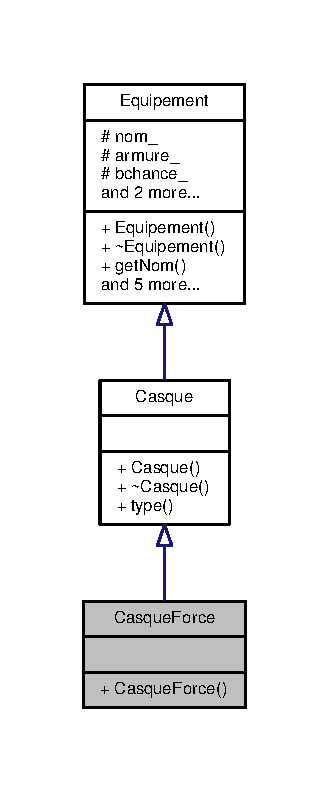
\includegraphics[width=158pt]{class_casque_force__inherit__graph}
\end{center}
\end{figure}


Graphe de collaboration de Casque\-Force\-:
\nopagebreak
\begin{figure}[H]
\begin{center}
\leavevmode
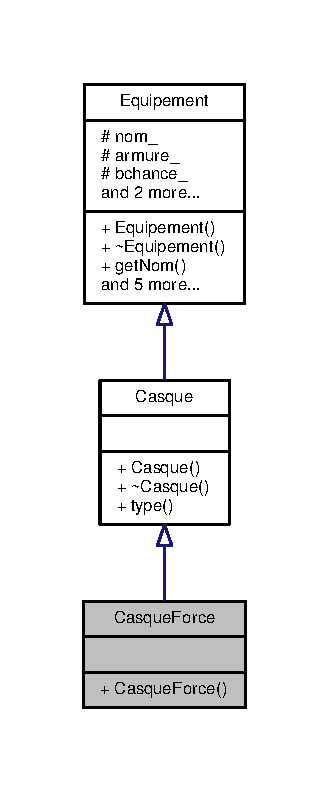
\includegraphics[width=158pt]{class_casque_force__coll__graph}
\end{center}
\end{figure}
\subsection*{Fonctions membres publiques}
\begin{DoxyCompactItemize}
\item 
int \hyperlink{class_casque_acb93c4c89d61c945d75ee3d47bede861}{type} ()
\begin{DoxyCompactList}\small\item\em Renvoie le type de l'equipement. \end{DoxyCompactList}\item 
virtual std\-::string \hyperlink{class_equipement_a0b0426a70bfce6e7c3efac605b75cd8e}{get\-Nom} ()
\begin{DoxyCompactList}\small\item\em Retourne le nom de l'equipement. \end{DoxyCompactList}\item 
virtual int \hyperlink{class_equipement_aabcf10fd762945fa4a37a9cf8321f463}{get\-Bforce} ()
\begin{DoxyCompactList}\small\item\em Retourne le bonus de force. \end{DoxyCompactList}\item 
virtual int \hyperlink{class_equipement_ad9fd7528c4f181970b7a0877f4145f89}{get\-Bvie} ()
\begin{DoxyCompactList}\small\item\em Retourne le bonus de vie. \end{DoxyCompactList}\item 
virtual int \hyperlink{class_equipement_a73485135eacdf30d5f49c9e34e5f4d0e}{get\-Bchance} ()
\begin{DoxyCompactList}\small\item\em Retourne le bonus de chance. \end{DoxyCompactList}\item 
virtual int \hyperlink{class_equipement_a8577d49fd00b8effa39388feccb29901}{get\-Armure} ()
\begin{DoxyCompactList}\small\item\em Retourne l'armure fournie par l'equipement. \end{DoxyCompactList}\end{DoxyCompactItemize}
\subsection*{Attributs protégés}
\begin{DoxyCompactItemize}
\item 
\hypertarget{class_equipement_a930290aac01ecd40c7a646ab8f66d742}{std\-::string {\bfseries nom\-\_\-}}\label{class_equipement_a930290aac01ecd40c7a646ab8f66d742}

\item 
\hypertarget{class_equipement_a69339ce4f1f5fe7e6fcdeda5b74c14a4}{int {\bfseries armure\-\_\-}}\label{class_equipement_a69339ce4f1f5fe7e6fcdeda5b74c14a4}

\item 
\hypertarget{class_equipement_aa70effa6a8144fe1f4fe874af7139793}{int {\bfseries bchance\-\_\-}}\label{class_equipement_aa70effa6a8144fe1f4fe874af7139793}

\item 
\hypertarget{class_equipement_a73ac5bff40e3f6bf1d8e6f0e524e750f}{int {\bfseries bvie\-\_\-}}\label{class_equipement_a73ac5bff40e3f6bf1d8e6f0e524e750f}

\item 
\hypertarget{class_equipement_af87cf3f291386d5401be6994dd8fb8be}{int {\bfseries bforce\-\_\-}}\label{class_equipement_af87cf3f291386d5401be6994dd8fb8be}

\end{DoxyCompactItemize}


\subsection{Description détaillée}
\hyperlink{class_casque_force}{Casque\-Force} herite de \hyperlink{class_casque}{Casque}. 

\subsection{Documentation des fonctions membres}
\hypertarget{class_equipement_a8577d49fd00b8effa39388feccb29901}{\index{Casque\-Force@{Casque\-Force}!get\-Armure@{get\-Armure}}
\index{get\-Armure@{get\-Armure}!CasqueForce@{Casque\-Force}}
\subsubsection[{get\-Armure}]{\setlength{\rightskip}{0pt plus 5cm}int Equipement\-::get\-Armure (
\begin{DoxyParamCaption}
{}
\end{DoxyParamCaption}
)\hspace{0.3cm}{\ttfamily [virtual]}, {\ttfamily [inherited]}}}\label{class_equipement_a8577d49fd00b8effa39388feccb29901}


Retourne l'armure fournie par l'equipement. 

\begin{DoxyReturn}{Renvoie}
armure 
\end{DoxyReturn}


Réimplémentée dans \hyperlink{class_d_equip_a7b2c8227ae884c23ccc8f3a2e5702186}{D\-Equip}.

\hypertarget{class_equipement_a73485135eacdf30d5f49c9e34e5f4d0e}{\index{Casque\-Force@{Casque\-Force}!get\-Bchance@{get\-Bchance}}
\index{get\-Bchance@{get\-Bchance}!CasqueForce@{Casque\-Force}}
\subsubsection[{get\-Bchance}]{\setlength{\rightskip}{0pt plus 5cm}int Equipement\-::get\-Bchance (
\begin{DoxyParamCaption}
{}
\end{DoxyParamCaption}
)\hspace{0.3cm}{\ttfamily [virtual]}, {\ttfamily [inherited]}}}\label{class_equipement_a73485135eacdf30d5f49c9e34e5f4d0e}


Retourne le bonus de chance. 

\begin{DoxyReturn}{Renvoie}
Bchance 
\end{DoxyReturn}


Réimplémentée dans \hyperlink{class_d_equip_a39407c92f0de87306a33f57fd22ce997}{D\-Equip}.

\hypertarget{class_equipement_aabcf10fd762945fa4a37a9cf8321f463}{\index{Casque\-Force@{Casque\-Force}!get\-Bforce@{get\-Bforce}}
\index{get\-Bforce@{get\-Bforce}!CasqueForce@{Casque\-Force}}
\subsubsection[{get\-Bforce}]{\setlength{\rightskip}{0pt plus 5cm}int Equipement\-::get\-Bforce (
\begin{DoxyParamCaption}
{}
\end{DoxyParamCaption}
)\hspace{0.3cm}{\ttfamily [virtual]}, {\ttfamily [inherited]}}}\label{class_equipement_aabcf10fd762945fa4a37a9cf8321f463}


Retourne le bonus de force. 

\begin{DoxyReturn}{Renvoie}
Bforce 
\end{DoxyReturn}


Réimplémentée dans \hyperlink{class_d_equip_adb6645ce01c12a4cb3fe0b522ea6b25e}{D\-Equip}.

\hypertarget{class_equipement_ad9fd7528c4f181970b7a0877f4145f89}{\index{Casque\-Force@{Casque\-Force}!get\-Bvie@{get\-Bvie}}
\index{get\-Bvie@{get\-Bvie}!CasqueForce@{Casque\-Force}}
\subsubsection[{get\-Bvie}]{\setlength{\rightskip}{0pt plus 5cm}int Equipement\-::get\-Bvie (
\begin{DoxyParamCaption}
{}
\end{DoxyParamCaption}
)\hspace{0.3cm}{\ttfamily [virtual]}, {\ttfamily [inherited]}}}\label{class_equipement_ad9fd7528c4f181970b7a0877f4145f89}


Retourne le bonus de vie. 

\begin{DoxyReturn}{Renvoie}
Bvie 
\end{DoxyReturn}


Réimplémentée dans \hyperlink{class_d_equip_a085ea4ac21c238d8c147ff4e6d74794f}{D\-Equip}.

\hypertarget{class_equipement_a0b0426a70bfce6e7c3efac605b75cd8e}{\index{Casque\-Force@{Casque\-Force}!get\-Nom@{get\-Nom}}
\index{get\-Nom@{get\-Nom}!CasqueForce@{Casque\-Force}}
\subsubsection[{get\-Nom}]{\setlength{\rightskip}{0pt plus 5cm}std\-::string Equipement\-::get\-Nom (
\begin{DoxyParamCaption}
{}
\end{DoxyParamCaption}
)\hspace{0.3cm}{\ttfamily [virtual]}, {\ttfamily [inherited]}}}\label{class_equipement_a0b0426a70bfce6e7c3efac605b75cd8e}


Retourne le nom de l'equipement. 

\begin{DoxyReturn}{Renvoie}
Nom 
\end{DoxyReturn}
\hypertarget{class_casque_acb93c4c89d61c945d75ee3d47bede861}{\index{Casque\-Force@{Casque\-Force}!type@{type}}
\index{type@{type}!CasqueForce@{Casque\-Force}}
\subsubsection[{type}]{\setlength{\rightskip}{0pt plus 5cm}int Casque\-::type (
\begin{DoxyParamCaption}
{}
\end{DoxyParamCaption}
)\hspace{0.3cm}{\ttfamily [virtual]}, {\ttfamily [inherited]}}}\label{class_casque_acb93c4c89d61c945d75ee3d47bede861}


Renvoie le type de l'equipement. 

\begin{DoxyReturn}{Renvoie}
int 
\end{DoxyReturn}


Implémente \hyperlink{class_equipement_a05b2c9d4cf22b6aefb6603fa4e322aa2}{Equipement}.


\hypertarget{class_casque_vie}{\section{Référence de la classe Casque\-Vie}
\label{class_casque_vie}\index{Casque\-Vie@{Casque\-Vie}}
}


\hyperlink{class_casque_vie}{Casque\-Vie} herite de \hyperlink{class_casque}{Casque}.  




Graphe d'héritage de Casque\-Vie\-:
\nopagebreak
\begin{figure}[H]
\begin{center}
\leavevmode
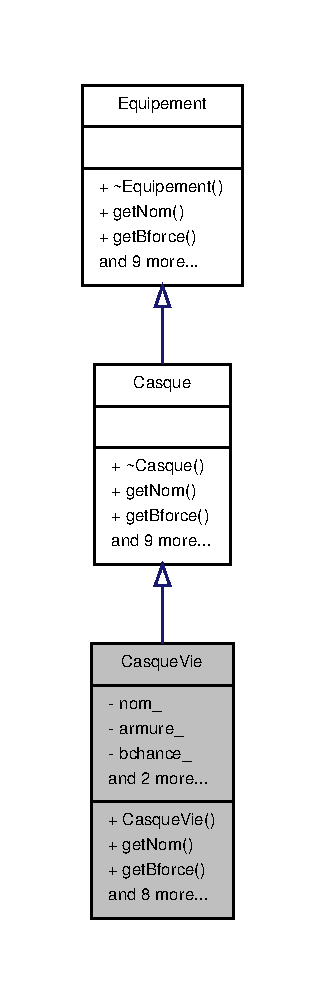
\includegraphics[width=156pt]{class_casque_vie__inherit__graph}
\end{center}
\end{figure}


Graphe de collaboration de Casque\-Vie\-:
\nopagebreak
\begin{figure}[H]
\begin{center}
\leavevmode
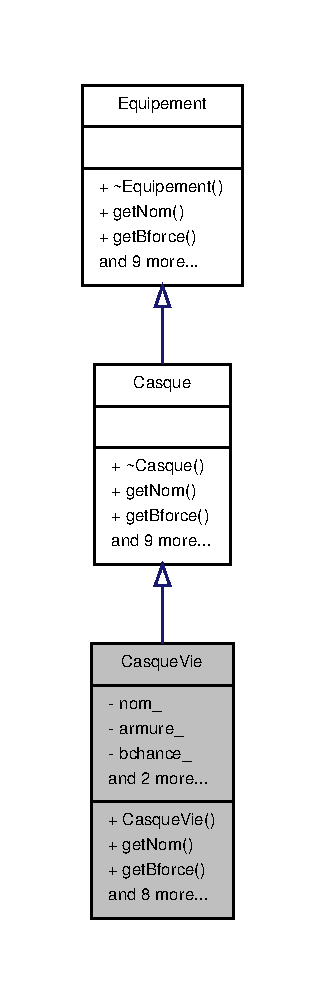
\includegraphics[width=156pt]{class_casque_vie__coll__graph}
\end{center}
\end{figure}
\subsection*{Fonctions membres publiques}
\begin{DoxyCompactItemize}
\item 
int \hyperlink{class_casque_acb93c4c89d61c945d75ee3d47bede861}{type} ()
\begin{DoxyCompactList}\small\item\em Renvoie le type de l'equipement. \end{DoxyCompactList}\item 
virtual std\-::string \hyperlink{class_equipement_a0b0426a70bfce6e7c3efac605b75cd8e}{get\-Nom} ()
\begin{DoxyCompactList}\small\item\em Retourne le nom de l'equipement. \end{DoxyCompactList}\item 
virtual int \hyperlink{class_equipement_aabcf10fd762945fa4a37a9cf8321f463}{get\-Bforce} ()
\begin{DoxyCompactList}\small\item\em Retourne le bonus de force. \end{DoxyCompactList}\item 
virtual int \hyperlink{class_equipement_ad9fd7528c4f181970b7a0877f4145f89}{get\-Bvie} ()
\begin{DoxyCompactList}\small\item\em Retourne le bonus de vie. \end{DoxyCompactList}\item 
virtual int \hyperlink{class_equipement_a73485135eacdf30d5f49c9e34e5f4d0e}{get\-Bchance} ()
\begin{DoxyCompactList}\small\item\em Retourne le bonus de chance. \end{DoxyCompactList}\item 
virtual int \hyperlink{class_equipement_a8577d49fd00b8effa39388feccb29901}{get\-Armure} ()
\begin{DoxyCompactList}\small\item\em Retourne l'armure fournie par l'equipement. \end{DoxyCompactList}\end{DoxyCompactItemize}
\subsection*{Attributs protégés}
\begin{DoxyCompactItemize}
\item 
\hypertarget{class_equipement_a930290aac01ecd40c7a646ab8f66d742}{std\-::string {\bfseries nom\-\_\-}}\label{class_equipement_a930290aac01ecd40c7a646ab8f66d742}

\item 
\hypertarget{class_equipement_a69339ce4f1f5fe7e6fcdeda5b74c14a4}{int {\bfseries armure\-\_\-}}\label{class_equipement_a69339ce4f1f5fe7e6fcdeda5b74c14a4}

\item 
\hypertarget{class_equipement_aa70effa6a8144fe1f4fe874af7139793}{int {\bfseries bchance\-\_\-}}\label{class_equipement_aa70effa6a8144fe1f4fe874af7139793}

\item 
\hypertarget{class_equipement_a73ac5bff40e3f6bf1d8e6f0e524e750f}{int {\bfseries bvie\-\_\-}}\label{class_equipement_a73ac5bff40e3f6bf1d8e6f0e524e750f}

\item 
\hypertarget{class_equipement_af87cf3f291386d5401be6994dd8fb8be}{int {\bfseries bforce\-\_\-}}\label{class_equipement_af87cf3f291386d5401be6994dd8fb8be}

\end{DoxyCompactItemize}


\subsection{Description détaillée}
\hyperlink{class_casque_vie}{Casque\-Vie} herite de \hyperlink{class_casque}{Casque}. 

\subsection{Documentation des fonctions membres}
\hypertarget{class_equipement_a8577d49fd00b8effa39388feccb29901}{\index{Casque\-Vie@{Casque\-Vie}!get\-Armure@{get\-Armure}}
\index{get\-Armure@{get\-Armure}!CasqueVie@{Casque\-Vie}}
\subsubsection[{get\-Armure}]{\setlength{\rightskip}{0pt plus 5cm}int Equipement\-::get\-Armure (
\begin{DoxyParamCaption}
{}
\end{DoxyParamCaption}
)\hspace{0.3cm}{\ttfamily [virtual]}, {\ttfamily [inherited]}}}\label{class_equipement_a8577d49fd00b8effa39388feccb29901}


Retourne l'armure fournie par l'equipement. 

\begin{DoxyReturn}{Renvoie}
armure 
\end{DoxyReturn}


Réimplémentée dans \hyperlink{class_d_equip_a7b2c8227ae884c23ccc8f3a2e5702186}{D\-Equip}.

\hypertarget{class_equipement_a73485135eacdf30d5f49c9e34e5f4d0e}{\index{Casque\-Vie@{Casque\-Vie}!get\-Bchance@{get\-Bchance}}
\index{get\-Bchance@{get\-Bchance}!CasqueVie@{Casque\-Vie}}
\subsubsection[{get\-Bchance}]{\setlength{\rightskip}{0pt plus 5cm}int Equipement\-::get\-Bchance (
\begin{DoxyParamCaption}
{}
\end{DoxyParamCaption}
)\hspace{0.3cm}{\ttfamily [virtual]}, {\ttfamily [inherited]}}}\label{class_equipement_a73485135eacdf30d5f49c9e34e5f4d0e}


Retourne le bonus de chance. 

\begin{DoxyReturn}{Renvoie}
Bchance 
\end{DoxyReturn}


Réimplémentée dans \hyperlink{class_d_equip_a39407c92f0de87306a33f57fd22ce997}{D\-Equip}.

\hypertarget{class_equipement_aabcf10fd762945fa4a37a9cf8321f463}{\index{Casque\-Vie@{Casque\-Vie}!get\-Bforce@{get\-Bforce}}
\index{get\-Bforce@{get\-Bforce}!CasqueVie@{Casque\-Vie}}
\subsubsection[{get\-Bforce}]{\setlength{\rightskip}{0pt plus 5cm}int Equipement\-::get\-Bforce (
\begin{DoxyParamCaption}
{}
\end{DoxyParamCaption}
)\hspace{0.3cm}{\ttfamily [virtual]}, {\ttfamily [inherited]}}}\label{class_equipement_aabcf10fd762945fa4a37a9cf8321f463}


Retourne le bonus de force. 

\begin{DoxyReturn}{Renvoie}
Bforce 
\end{DoxyReturn}


Réimplémentée dans \hyperlink{class_d_equip_adb6645ce01c12a4cb3fe0b522ea6b25e}{D\-Equip}.

\hypertarget{class_equipement_ad9fd7528c4f181970b7a0877f4145f89}{\index{Casque\-Vie@{Casque\-Vie}!get\-Bvie@{get\-Bvie}}
\index{get\-Bvie@{get\-Bvie}!CasqueVie@{Casque\-Vie}}
\subsubsection[{get\-Bvie}]{\setlength{\rightskip}{0pt plus 5cm}int Equipement\-::get\-Bvie (
\begin{DoxyParamCaption}
{}
\end{DoxyParamCaption}
)\hspace{0.3cm}{\ttfamily [virtual]}, {\ttfamily [inherited]}}}\label{class_equipement_ad9fd7528c4f181970b7a0877f4145f89}


Retourne le bonus de vie. 

\begin{DoxyReturn}{Renvoie}
Bvie 
\end{DoxyReturn}


Réimplémentée dans \hyperlink{class_d_equip_a085ea4ac21c238d8c147ff4e6d74794f}{D\-Equip}.

\hypertarget{class_equipement_a0b0426a70bfce6e7c3efac605b75cd8e}{\index{Casque\-Vie@{Casque\-Vie}!get\-Nom@{get\-Nom}}
\index{get\-Nom@{get\-Nom}!CasqueVie@{Casque\-Vie}}
\subsubsection[{get\-Nom}]{\setlength{\rightskip}{0pt plus 5cm}std\-::string Equipement\-::get\-Nom (
\begin{DoxyParamCaption}
{}
\end{DoxyParamCaption}
)\hspace{0.3cm}{\ttfamily [virtual]}, {\ttfamily [inherited]}}}\label{class_equipement_a0b0426a70bfce6e7c3efac605b75cd8e}


Retourne le nom de l'equipement. 

\begin{DoxyReturn}{Renvoie}
Nom 
\end{DoxyReturn}
\hypertarget{class_casque_acb93c4c89d61c945d75ee3d47bede861}{\index{Casque\-Vie@{Casque\-Vie}!type@{type}}
\index{type@{type}!CasqueVie@{Casque\-Vie}}
\subsubsection[{type}]{\setlength{\rightskip}{0pt plus 5cm}int Casque\-::type (
\begin{DoxyParamCaption}
{}
\end{DoxyParamCaption}
)\hspace{0.3cm}{\ttfamily [virtual]}, {\ttfamily [inherited]}}}\label{class_casque_acb93c4c89d61c945d75ee3d47bede861}


Renvoie le type de l'equipement. 

\begin{DoxyReturn}{Renvoie}
int 
\end{DoxyReturn}


Implémente \hyperlink{class_equipement_a05b2c9d4cf22b6aefb6603fa4e322aa2}{Equipement}.


\section{Référence de la classe Chance\-Factory}
\label{class_chance_factory}\index{Chance\-Factory@{Chance\-Factory}}


Graphe d'héritage de Chance\-Factory\-:\nopagebreak
\begin{figure}[H]
\begin{center}
\leavevmode
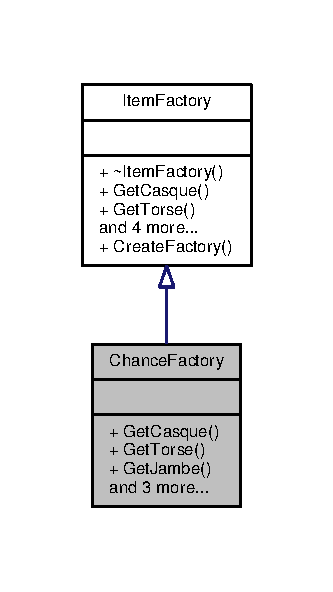
\includegraphics[width=160pt]{class_chance_factory__inherit__graph}
\end{center}
\end{figure}


Graphe de collaboration de Chance\-Factory\-:\nopagebreak
\begin{figure}[H]
\begin{center}
\leavevmode
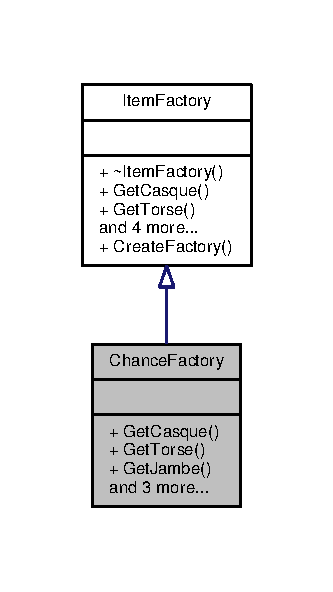
\includegraphics[width=160pt]{class_chance_factory__coll__graph}
\end{center}
\end{figure}
\subsection*{Fonctions membres publiques}
\begin{DoxyCompactItemize}
\item 
{\bf Casque} $\ast$ {\bf Get\-Casque} ()
\item 
{\bf Torse} $\ast$ {\bf Get\-Torse} ()
\item 
{\bf Jambe} $\ast$ {\bf Get\-Jambe} ()
\item 
{\bf Conso} $\ast$ {\bf Get\-Conso} ()
\item 
{\bf Epee} $\ast$ {\bf Get\-Epee} ()
\item 
{\bf Dague} $\ast$ {\bf Get\-Dague} ()
\item 
{\bf Hache} $\ast$ {\bf Get\-Hache} ()
\end{DoxyCompactItemize}
\subsection*{Fonctions membres publiques statiques}
\begin{DoxyCompactItemize}
\item 
static {\bf Item\-Factory} $\ast$ {\bf Create\-Factory} ({\bf I\-T\-E\-M\-\_\-\-F\-A\-C\-T\-O\-R\-I\-E\-S} factory)
\end{DoxyCompactItemize}


\subsection{Documentation des fonctions membres}
\index{Chance\-Factory@{Chance\-Factory}!Create\-Factory@{Create\-Factory}}
\index{Create\-Factory@{Create\-Factory}!ChanceFactory@{Chance\-Factory}}
\subsubsection[{Create\-Factory}]{\setlength{\rightskip}{0pt plus 5cm}static {\bf Item\-Factory}$\ast$ Item\-Factory\-::\-Create\-Factory (
\begin{DoxyParamCaption}
\item[{{\bf I\-T\-E\-M\-\_\-\-F\-A\-C\-T\-O\-R\-I\-E\-S}}]{factory}
\end{DoxyParamCaption}
)\hspace{0.3cm}{\ttfamily [static]}, {\ttfamily [inherited]}}\label{class_item_factory_a6b427dfb3c03771844365ec7c5db1fd7}
\index{Chance\-Factory@{Chance\-Factory}!Get\-Casque@{Get\-Casque}}
\index{Get\-Casque@{Get\-Casque}!ChanceFactory@{Chance\-Factory}}
\subsubsection[{Get\-Casque}]{\setlength{\rightskip}{0pt plus 5cm}{\bf Casque}$\ast$ Chance\-Factory\-::\-Get\-Casque (
\begin{DoxyParamCaption}
{}
\end{DoxyParamCaption}
)\hspace{0.3cm}{\ttfamily [virtual]}}\label{class_chance_factory_ab6fb002920a57729261ea6659576e164}


Implémente {\bf Item\-Factory} \doxyref{}{p.}{class_item_factory_a89450cf0176a8da74cc5a9b8ef5aaae6}.

\index{Chance\-Factory@{Chance\-Factory}!Get\-Conso@{Get\-Conso}}
\index{Get\-Conso@{Get\-Conso}!ChanceFactory@{Chance\-Factory}}
\subsubsection[{Get\-Conso}]{\setlength{\rightskip}{0pt plus 5cm}{\bf Conso}$\ast$ Chance\-Factory\-::\-Get\-Conso (
\begin{DoxyParamCaption}
{}
\end{DoxyParamCaption}
)\hspace{0.3cm}{\ttfamily [virtual]}}\label{class_chance_factory_aac6ef128121a2e046ffe71b66b4ed39f}


Implémente {\bf Item\-Factory} \doxyref{}{p.}{class_item_factory_a0db8489e85637bb3f3f7096401176d18}.

\index{Chance\-Factory@{Chance\-Factory}!Get\-Dague@{Get\-Dague}}
\index{Get\-Dague@{Get\-Dague}!ChanceFactory@{Chance\-Factory}}
\subsubsection[{Get\-Dague}]{\setlength{\rightskip}{0pt plus 5cm}{\bf Dague}$\ast$ Chance\-Factory\-::\-Get\-Dague (
\begin{DoxyParamCaption}
{}
\end{DoxyParamCaption}
)\hspace{0.3cm}{\ttfamily [virtual]}}\label{class_chance_factory_aafacb483e9f7c32e605051a3fca801a5}


Implémente {\bf Item\-Factory} \doxyref{}{p.}{class_item_factory_a65ed7c9978011812487e6b12b4155fbd}.

\index{Chance\-Factory@{Chance\-Factory}!Get\-Epee@{Get\-Epee}}
\index{Get\-Epee@{Get\-Epee}!ChanceFactory@{Chance\-Factory}}
\subsubsection[{Get\-Epee}]{\setlength{\rightskip}{0pt plus 5cm}{\bf Epee}$\ast$ Chance\-Factory\-::\-Get\-Epee (
\begin{DoxyParamCaption}
{}
\end{DoxyParamCaption}
)\hspace{0.3cm}{\ttfamily [virtual]}}\label{class_chance_factory_a33a21a5142f67cc0218fa14b70520480}


Implémente {\bf Item\-Factory} \doxyref{}{p.}{class_item_factory_a8a413e61bf23ad24a549382e4e4e396f}.

\index{Chance\-Factory@{Chance\-Factory}!Get\-Hache@{Get\-Hache}}
\index{Get\-Hache@{Get\-Hache}!ChanceFactory@{Chance\-Factory}}
\subsubsection[{Get\-Hache}]{\setlength{\rightskip}{0pt plus 5cm}{\bf Hache}$\ast$ Chance\-Factory\-::\-Get\-Hache (
\begin{DoxyParamCaption}
{}
\end{DoxyParamCaption}
)\hspace{0.3cm}{\ttfamily [virtual]}}\label{class_chance_factory_a08105f8893159dc811dfa6f650321784}


Implémente {\bf Item\-Factory} \doxyref{}{p.}{class_item_factory_afd402df71468d0a96ea12e92c80a185e}.

\index{Chance\-Factory@{Chance\-Factory}!Get\-Jambe@{Get\-Jambe}}
\index{Get\-Jambe@{Get\-Jambe}!ChanceFactory@{Chance\-Factory}}
\subsubsection[{Get\-Jambe}]{\setlength{\rightskip}{0pt plus 5cm}{\bf Jambe}$\ast$ Chance\-Factory\-::\-Get\-Jambe (
\begin{DoxyParamCaption}
{}
\end{DoxyParamCaption}
)\hspace{0.3cm}{\ttfamily [virtual]}}\label{class_chance_factory_ac94fa9b411f7489c8d362dce13ee0370}


Implémente {\bf Item\-Factory} \doxyref{}{p.}{class_item_factory_a0a9cc8a72f93f260a61d393d8fb76012}.

\index{Chance\-Factory@{Chance\-Factory}!Get\-Torse@{Get\-Torse}}
\index{Get\-Torse@{Get\-Torse}!ChanceFactory@{Chance\-Factory}}
\subsubsection[{Get\-Torse}]{\setlength{\rightskip}{0pt plus 5cm}{\bf Torse}$\ast$ Chance\-Factory\-::\-Get\-Torse (
\begin{DoxyParamCaption}
{}
\end{DoxyParamCaption}
)\hspace{0.3cm}{\ttfamily [virtual]}}\label{class_chance_factory_a0e811061c4785372d75903f046cfd96d}


Implémente {\bf Item\-Factory} \doxyref{}{p.}{class_item_factory_ad5f3eb7dffeed5577e05e859775af3dd}.



La documentation de cette classe a été générée à partir du fichier suivant \-:\begin{DoxyCompactItemize}
\item 
src/{\bf Chance\-Factory.\-hpp}\end{DoxyCompactItemize}

\section{Référence de la classe Dague}
\label{class_dague}\index{Dague@{Dague}}


Graphe d'héritage de Dague\-:\nopagebreak
\begin{figure}[H]
\begin{center}
\leavevmode
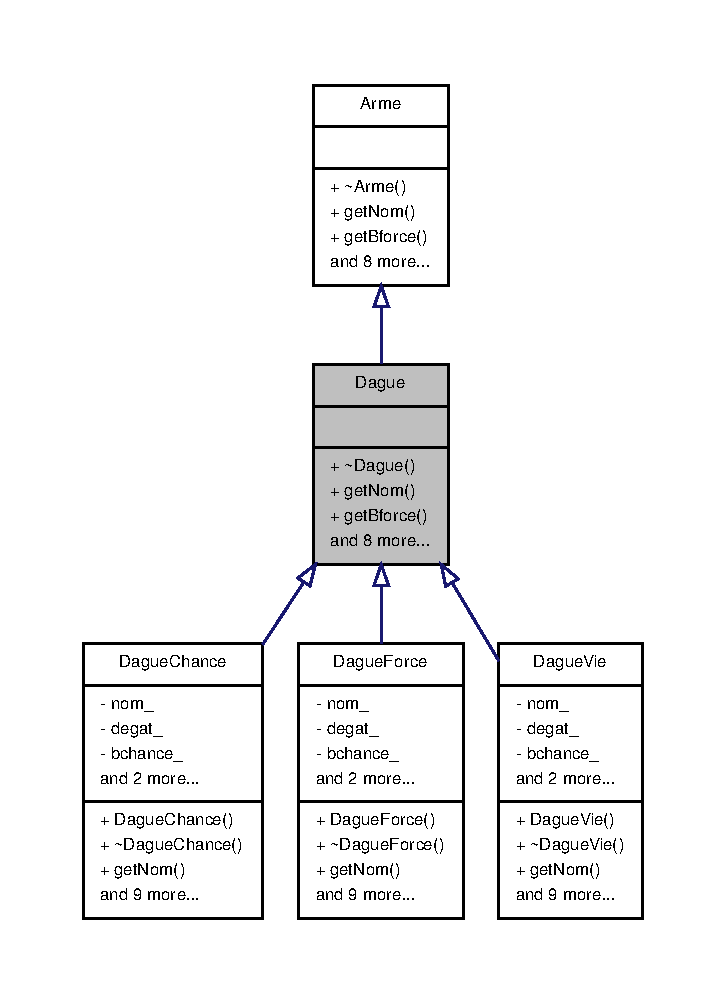
\includegraphics[width=348pt]{class_dague__inherit__graph}
\end{center}
\end{figure}


Graphe de collaboration de Dague\-:\nopagebreak
\begin{figure}[H]
\begin{center}
\leavevmode
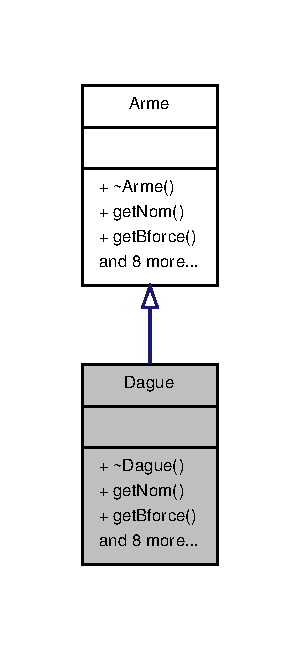
\includegraphics[width=144pt]{class_dague__coll__graph}
\end{center}
\end{figure}
\subsection*{Fonctions membres publiques}
\begin{DoxyCompactItemize}
\item 
virtual {\bf $\sim$\-Dague} ()
\item 
virtual std\-::string {\bf get\-Nom} ()=0
\item 
virtual int {\bf get\-Bforce} ()=0
\item 
virtual int {\bf get\-Bvie} ()=0
\item 
virtual int {\bf get\-Bchance} ()=0
\item 
virtual int {\bf get\-Degat} ()=0
\item 
virtual void {\bf set\-Bforce} (int bforce)=0
\item 
virtual void {\bf set\-Bvie} (int bvie)=0
\item 
virtual void {\bf set\-Bchance} (int bchance)=0
\item 
virtual void {\bf set\-Degat} (int degat)=0
\item 
virtual void {\bf set\-Nom} (std\-::string nom)=0
\end{DoxyCompactItemize}


\subsection{Documentation des constructeurs et destructeur}
\index{Dague@{Dague}!$\sim$\-Dague@{$\sim$\-Dague}}
\index{$\sim$\-Dague@{$\sim$\-Dague}!Dague@{Dague}}
\subsubsection[{$\sim$\-Dague}]{\setlength{\rightskip}{0pt plus 5cm}virtual Dague\-::$\sim$\-Dague (
\begin{DoxyParamCaption}
{}
\end{DoxyParamCaption}
)\hspace{0.3cm}{\ttfamily [inline]}, {\ttfamily [virtual]}}\label{class_dague_aae1729ae30677ce622b4f3eda7a36d75}


\subsection{Documentation des fonctions membres}
\index{Dague@{Dague}!get\-Bchance@{get\-Bchance}}
\index{get\-Bchance@{get\-Bchance}!Dague@{Dague}}
\subsubsection[{get\-Bchance}]{\setlength{\rightskip}{0pt plus 5cm}virtual int Dague\-::get\-Bchance (
\begin{DoxyParamCaption}
{}
\end{DoxyParamCaption}
)\hspace{0.3cm}{\ttfamily [pure virtual]}}\label{class_dague_a5de075bd307074a52d7676046ab40ea1}


Implémente {\bf Arme} \doxyref{}{p.}{class_arme_afcd4a79f4603cd9ced1eafd15be54316}.



Implémenté dans {\bf Dague\-Chance} \doxyref{}{p.}{class_dague_chance_ac6146c8ab45cd7d5f8c473f0c5a3f4ef}, {\bf Dague\-Force} \doxyref{}{p.}{class_dague_force_a65da3e61243d0e9f0710385a4b39b858}, et {\bf Dague\-Vie} \doxyref{}{p.}{class_dague_vie_ae42dfdf6833cfa9090cd42cbfe17d20c}.

\index{Dague@{Dague}!get\-Bforce@{get\-Bforce}}
\index{get\-Bforce@{get\-Bforce}!Dague@{Dague}}
\subsubsection[{get\-Bforce}]{\setlength{\rightskip}{0pt plus 5cm}virtual int Dague\-::get\-Bforce (
\begin{DoxyParamCaption}
{}
\end{DoxyParamCaption}
)\hspace{0.3cm}{\ttfamily [pure virtual]}}\label{class_dague_af9baa3478d3800f285bb961a73fb061f}


Implémente {\bf Arme} \doxyref{}{p.}{class_arme_a25da1859e12ebceb90283fb980f00758}.



Implémenté dans {\bf Dague\-Chance} \doxyref{}{p.}{class_dague_chance_ad5a65eb71a84fc9d9d081e94b6d88257}, {\bf Dague\-Force} \doxyref{}{p.}{class_dague_force_a5d8a8017647abdd63eb3bb4c0e87500f}, et {\bf Dague\-Vie} \doxyref{}{p.}{class_dague_vie_aab12c82cde51d11d83a465d9d076349f}.

\index{Dague@{Dague}!get\-Bvie@{get\-Bvie}}
\index{get\-Bvie@{get\-Bvie}!Dague@{Dague}}
\subsubsection[{get\-Bvie}]{\setlength{\rightskip}{0pt plus 5cm}virtual int Dague\-::get\-Bvie (
\begin{DoxyParamCaption}
{}
\end{DoxyParamCaption}
)\hspace{0.3cm}{\ttfamily [pure virtual]}}\label{class_dague_a35d0387f7d2249e7369b89f09427d36b}


Implémente {\bf Arme} \doxyref{}{p.}{class_arme_ad07794203a8fa685391cd6c107529aa1}.



Implémenté dans {\bf Dague\-Chance} \doxyref{}{p.}{class_dague_chance_a07dfcc6377639fdfe6a0ee6c4a8b3729}, {\bf Dague\-Force} \doxyref{}{p.}{class_dague_force_a15abc56ba8ea78cc3ed476af5b8820a0}, et {\bf Dague\-Vie} \doxyref{}{p.}{class_dague_vie_a751a65bab6845a4e1cf706e2d575ae23}.

\index{Dague@{Dague}!get\-Degat@{get\-Degat}}
\index{get\-Degat@{get\-Degat}!Dague@{Dague}}
\subsubsection[{get\-Degat}]{\setlength{\rightskip}{0pt plus 5cm}virtual int Dague\-::get\-Degat (
\begin{DoxyParamCaption}
{}
\end{DoxyParamCaption}
)\hspace{0.3cm}{\ttfamily [pure virtual]}}\label{class_dague_a25298dd54ed21b88ff1694962711028f}


Implémente {\bf Arme} \doxyref{}{p.}{class_arme_a93e1b6f8c800359c7651b2fc456a3ee1}.



Implémenté dans {\bf Dague\-Chance} \doxyref{}{p.}{class_dague_chance_acfff9ba3d01879aa998c4eb75724bec4}, {\bf Dague\-Force} \doxyref{}{p.}{class_dague_force_adb3447fe7c3670566a032f476334c1d5}, et {\bf Dague\-Vie} \doxyref{}{p.}{class_dague_vie_a5290ff3924ec192fbdc9b763d329bb39}.

\index{Dague@{Dague}!get\-Nom@{get\-Nom}}
\index{get\-Nom@{get\-Nom}!Dague@{Dague}}
\subsubsection[{get\-Nom}]{\setlength{\rightskip}{0pt plus 5cm}virtual std\-::string Dague\-::get\-Nom (
\begin{DoxyParamCaption}
{}
\end{DoxyParamCaption}
)\hspace{0.3cm}{\ttfamily [pure virtual]}}\label{class_dague_a4ac0c92d71164c8a9e54e626602d49ac}


Implémente {\bf Arme} \doxyref{}{p.}{class_arme_a0b6a30975be57770c6cae357b52395a0}.



Implémenté dans {\bf Dague\-Chance} \doxyref{}{p.}{class_dague_chance_a955ed40b9c57d721de4e4994ff47ed9d}, {\bf Dague\-Force} \doxyref{}{p.}{class_dague_force_aaee0493fa04f2633edb9d383a5997243}, et {\bf Dague\-Vie} \doxyref{}{p.}{class_dague_vie_a42d8393844d6f9d81759624be1a4edbc}.

\index{Dague@{Dague}!set\-Bchance@{set\-Bchance}}
\index{set\-Bchance@{set\-Bchance}!Dague@{Dague}}
\subsubsection[{set\-Bchance}]{\setlength{\rightskip}{0pt plus 5cm}virtual void Dague\-::set\-Bchance (
\begin{DoxyParamCaption}
\item[{int}]{bchance}
\end{DoxyParamCaption}
)\hspace{0.3cm}{\ttfamily [pure virtual]}}\label{class_dague_ae58691c16eebd09f03aac47c3b70d869}


Implémente {\bf Arme} \doxyref{}{p.}{class_arme_a27aa7d294d01ea38975841ea680a815a}.



Implémenté dans {\bf Dague\-Chance} \doxyref{}{p.}{class_dague_chance_a492f6549765cb10511d4dd7213036995}, {\bf Dague\-Force} \doxyref{}{p.}{class_dague_force_a291dc10a8c54d528b8ef2391963ee29f}, et {\bf Dague\-Vie} \doxyref{}{p.}{class_dague_vie_a6a78fd29aecba8f468106dc434c68648}.

\index{Dague@{Dague}!set\-Bforce@{set\-Bforce}}
\index{set\-Bforce@{set\-Bforce}!Dague@{Dague}}
\subsubsection[{set\-Bforce}]{\setlength{\rightskip}{0pt plus 5cm}virtual void Dague\-::set\-Bforce (
\begin{DoxyParamCaption}
\item[{int}]{bforce}
\end{DoxyParamCaption}
)\hspace{0.3cm}{\ttfamily [pure virtual]}}\label{class_dague_aff6198d6598ae0e1e142aed959d1a150}


Implémente {\bf Arme} \doxyref{}{p.}{class_arme_a8806ba4300d435ebe71bb4b9829296e8}.



Implémenté dans {\bf Dague\-Chance} \doxyref{}{p.}{class_dague_chance_ac2fd0b9d309ba0c335305ecdf57fa56b}, {\bf Dague\-Force} \doxyref{}{p.}{class_dague_force_aac379e382d25e38bf77b91e3c3ab2424}, et {\bf Dague\-Vie} \doxyref{}{p.}{class_dague_vie_a3fcf25af8aabbdea4a11a9386a020c9d}.

\index{Dague@{Dague}!set\-Bvie@{set\-Bvie}}
\index{set\-Bvie@{set\-Bvie}!Dague@{Dague}}
\subsubsection[{set\-Bvie}]{\setlength{\rightskip}{0pt plus 5cm}virtual void Dague\-::set\-Bvie (
\begin{DoxyParamCaption}
\item[{int}]{bvie}
\end{DoxyParamCaption}
)\hspace{0.3cm}{\ttfamily [pure virtual]}}\label{class_dague_adb4c176caf63fb57a4012c104f0bf35b}


Implémente {\bf Arme} \doxyref{}{p.}{class_arme_a0580ea53e4254942a4ef82aec8706ead}.



Implémenté dans {\bf Dague\-Chance} \doxyref{}{p.}{class_dague_chance_a3cc292f96dc5a7f2f2b9c313e1909f2e}, {\bf Dague\-Force} \doxyref{}{p.}{class_dague_force_a9cd47a8d709119faa983f40e986afa1f}, et {\bf Dague\-Vie} \doxyref{}{p.}{class_dague_vie_ac172f87953d202cc839acb687ba8f504}.

\index{Dague@{Dague}!set\-Degat@{set\-Degat}}
\index{set\-Degat@{set\-Degat}!Dague@{Dague}}
\subsubsection[{set\-Degat}]{\setlength{\rightskip}{0pt plus 5cm}virtual void Dague\-::set\-Degat (
\begin{DoxyParamCaption}
\item[{int}]{degat}
\end{DoxyParamCaption}
)\hspace{0.3cm}{\ttfamily [pure virtual]}}\label{class_dague_a14c7a619bb8c4dfd54c3b198b303821d}


Implémente {\bf Arme} \doxyref{}{p.}{class_arme_a2e2cd008885e4ba4dca346905e7e5f73}.



Implémenté dans {\bf Dague\-Chance} \doxyref{}{p.}{class_dague_chance_a61b3084db9375853a1f60e99ad584afe}, {\bf Dague\-Force} \doxyref{}{p.}{class_dague_force_a3b4d211b9f6c67ab7cfb76051b143dea}, et {\bf Dague\-Vie} \doxyref{}{p.}{class_dague_vie_adab4e95d5f1b30ac3a43c5832f67c942}.

\index{Dague@{Dague}!set\-Nom@{set\-Nom}}
\index{set\-Nom@{set\-Nom}!Dague@{Dague}}
\subsubsection[{set\-Nom}]{\setlength{\rightskip}{0pt plus 5cm}virtual void Dague\-::set\-Nom (
\begin{DoxyParamCaption}
\item[{std\-::string}]{nom}
\end{DoxyParamCaption}
)\hspace{0.3cm}{\ttfamily [pure virtual]}}\label{class_dague_a5b5f19a4e51c2fb13cbf320044e87697}


Implémente {\bf Arme} \doxyref{}{p.}{class_arme_a561f12b90bd01d26328541ba54f6aaa6}.



Implémenté dans {\bf Dague\-Chance} \doxyref{}{p.}{class_dague_chance_a79bcbf32965ad2a43b32c86fc630d60f}, {\bf Dague\-Force} \doxyref{}{p.}{class_dague_force_ac5a74a106d950a5e0ae77a083dd4c235}, et {\bf Dague\-Vie} \doxyref{}{p.}{class_dague_vie_ad99195a86efd066f81b46c44a645696f}.



La documentation de cette classe a été générée à partir du fichier suivant \-:\begin{DoxyCompactItemize}
\item 
src/{\bf Dague.\-hpp}\end{DoxyCompactItemize}

\section{Référence de la classe Dague\-Chance}
\label{class_dague_chance}\index{Dague\-Chance@{Dague\-Chance}}


Graphe d'héritage de Dague\-Chance\-:\nopagebreak
\begin{figure}[H]
\begin{center}
\leavevmode
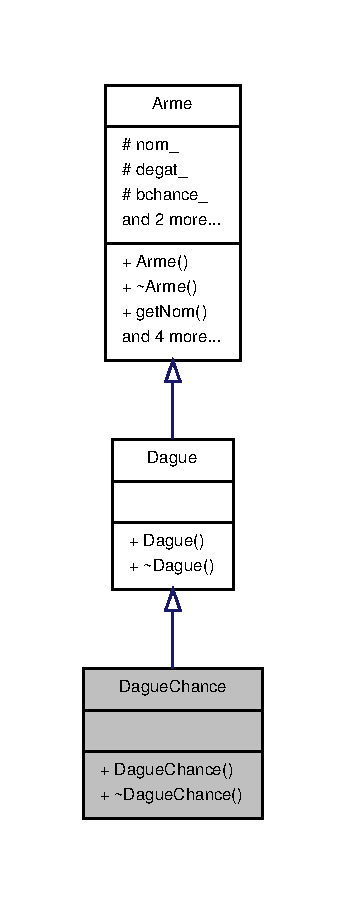
\includegraphics[width=166pt]{class_dague_chance__inherit__graph}
\end{center}
\end{figure}


Graphe de collaboration de Dague\-Chance\-:\nopagebreak
\begin{figure}[H]
\begin{center}
\leavevmode
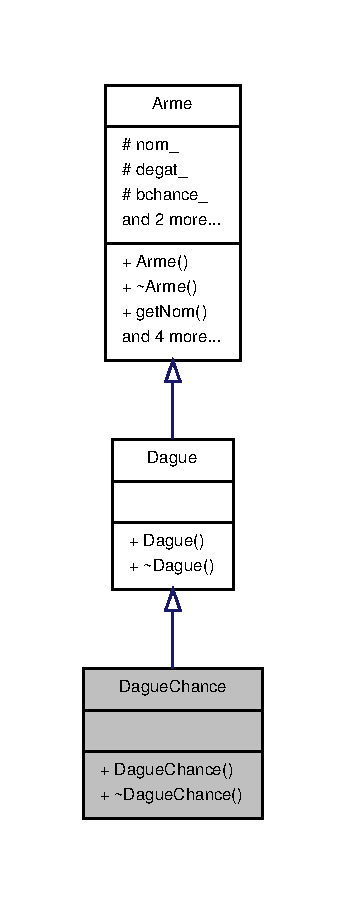
\includegraphics[width=166pt]{class_dague_chance__coll__graph}
\end{center}
\end{figure}
\subsection*{Fonctions membres publiques}
\begin{DoxyCompactItemize}
\item 
{\bf Dague\-Chance} ()
\item 
{\bf $\sim$\-Dague\-Chance} ()
\item 
std\-::string {\bf get\-Nom} ()
\item 
int {\bf get\-Bforce} ()
\item 
int {\bf get\-Bvie} ()
\item 
int {\bf get\-Bchance} ()
\item 
int {\bf get\-Degat} ()
\item 
void {\bf set\-Bforce} (int bforce)
\item 
void {\bf set\-Bvie} (int bvie)
\item 
void {\bf set\-Bchance} (int bchance)
\item 
void {\bf set\-Degat} (int degat)
\item 
void {\bf set\-Nom} (std\-::string nom)
\end{DoxyCompactItemize}
\subsection*{Attributs privés}
\begin{DoxyCompactItemize}
\item 
std\-::string {\bf nom\-\_\-}
\item 
int {\bf degat\-\_\-}
\item 
int {\bf bchance\-\_\-}
\item 
int {\bf bvie\-\_\-}
\item 
int {\bf bforce\-\_\-}
\end{DoxyCompactItemize}


\subsection{Documentation des constructeurs et destructeur}
\index{Dague\-Chance@{Dague\-Chance}!Dague\-Chance@{Dague\-Chance}}
\index{Dague\-Chance@{Dague\-Chance}!DagueChance@{Dague\-Chance}}
\subsubsection[{Dague\-Chance}]{\setlength{\rightskip}{0pt plus 5cm}Dague\-Chance\-::\-Dague\-Chance (
\begin{DoxyParamCaption}
{}
\end{DoxyParamCaption}
)}\label{class_dague_chance_af071f6a8261236cb1bad73d859008ad1}
\index{Dague\-Chance@{Dague\-Chance}!$\sim$\-Dague\-Chance@{$\sim$\-Dague\-Chance}}
\index{$\sim$\-Dague\-Chance@{$\sim$\-Dague\-Chance}!DagueChance@{Dague\-Chance}}
\subsubsection[{$\sim$\-Dague\-Chance}]{\setlength{\rightskip}{0pt plus 5cm}Dague\-Chance\-::$\sim$\-Dague\-Chance (
\begin{DoxyParamCaption}
{}
\end{DoxyParamCaption}
)}\label{class_dague_chance_a2715ce013d9d2f415760a3ff8a7828dd}


\subsection{Documentation des fonctions membres}
\index{Dague\-Chance@{Dague\-Chance}!get\-Bchance@{get\-Bchance}}
\index{get\-Bchance@{get\-Bchance}!DagueChance@{Dague\-Chance}}
\subsubsection[{get\-Bchance}]{\setlength{\rightskip}{0pt plus 5cm}int Dague\-Chance\-::get\-Bchance (
\begin{DoxyParamCaption}
{}
\end{DoxyParamCaption}
)\hspace{0.3cm}{\ttfamily [virtual]}}\label{class_dague_chance_ac6146c8ab45cd7d5f8c473f0c5a3f4ef}


Implémente {\bf Dague} \doxyref{}{p.}{class_dague_a5de075bd307074a52d7676046ab40ea1}.

\index{Dague\-Chance@{Dague\-Chance}!get\-Bforce@{get\-Bforce}}
\index{get\-Bforce@{get\-Bforce}!DagueChance@{Dague\-Chance}}
\subsubsection[{get\-Bforce}]{\setlength{\rightskip}{0pt plus 5cm}int Dague\-Chance\-::get\-Bforce (
\begin{DoxyParamCaption}
{}
\end{DoxyParamCaption}
)\hspace{0.3cm}{\ttfamily [virtual]}}\label{class_dague_chance_ad5a65eb71a84fc9d9d081e94b6d88257}


Implémente {\bf Dague} \doxyref{}{p.}{class_dague_af9baa3478d3800f285bb961a73fb061f}.

\index{Dague\-Chance@{Dague\-Chance}!get\-Bvie@{get\-Bvie}}
\index{get\-Bvie@{get\-Bvie}!DagueChance@{Dague\-Chance}}
\subsubsection[{get\-Bvie}]{\setlength{\rightskip}{0pt plus 5cm}int Dague\-Chance\-::get\-Bvie (
\begin{DoxyParamCaption}
{}
\end{DoxyParamCaption}
)\hspace{0.3cm}{\ttfamily [virtual]}}\label{class_dague_chance_a07dfcc6377639fdfe6a0ee6c4a8b3729}


Implémente {\bf Dague} \doxyref{}{p.}{class_dague_a35d0387f7d2249e7369b89f09427d36b}.

\index{Dague\-Chance@{Dague\-Chance}!get\-Degat@{get\-Degat}}
\index{get\-Degat@{get\-Degat}!DagueChance@{Dague\-Chance}}
\subsubsection[{get\-Degat}]{\setlength{\rightskip}{0pt plus 5cm}int Dague\-Chance\-::get\-Degat (
\begin{DoxyParamCaption}
{}
\end{DoxyParamCaption}
)\hspace{0.3cm}{\ttfamily [virtual]}}\label{class_dague_chance_acfff9ba3d01879aa998c4eb75724bec4}


Implémente {\bf Dague} \doxyref{}{p.}{class_dague_a25298dd54ed21b88ff1694962711028f}.

\index{Dague\-Chance@{Dague\-Chance}!get\-Nom@{get\-Nom}}
\index{get\-Nom@{get\-Nom}!DagueChance@{Dague\-Chance}}
\subsubsection[{get\-Nom}]{\setlength{\rightskip}{0pt plus 5cm}std\-::string Dague\-Chance\-::get\-Nom (
\begin{DoxyParamCaption}
{}
\end{DoxyParamCaption}
)\hspace{0.3cm}{\ttfamily [virtual]}}\label{class_dague_chance_a955ed40b9c57d721de4e4994ff47ed9d}


Implémente {\bf Dague} \doxyref{}{p.}{class_dague_a4ac0c92d71164c8a9e54e626602d49ac}.

\index{Dague\-Chance@{Dague\-Chance}!set\-Bchance@{set\-Bchance}}
\index{set\-Bchance@{set\-Bchance}!DagueChance@{Dague\-Chance}}
\subsubsection[{set\-Bchance}]{\setlength{\rightskip}{0pt plus 5cm}void Dague\-Chance\-::set\-Bchance (
\begin{DoxyParamCaption}
\item[{int}]{bchance}
\end{DoxyParamCaption}
)\hspace{0.3cm}{\ttfamily [virtual]}}\label{class_dague_chance_a492f6549765cb10511d4dd7213036995}


Implémente {\bf Dague} \doxyref{}{p.}{class_dague_ae58691c16eebd09f03aac47c3b70d869}.

\index{Dague\-Chance@{Dague\-Chance}!set\-Bforce@{set\-Bforce}}
\index{set\-Bforce@{set\-Bforce}!DagueChance@{Dague\-Chance}}
\subsubsection[{set\-Bforce}]{\setlength{\rightskip}{0pt plus 5cm}void Dague\-Chance\-::set\-Bforce (
\begin{DoxyParamCaption}
\item[{int}]{bforce}
\end{DoxyParamCaption}
)\hspace{0.3cm}{\ttfamily [virtual]}}\label{class_dague_chance_ac2fd0b9d309ba0c335305ecdf57fa56b}


Implémente {\bf Dague} \doxyref{}{p.}{class_dague_aff6198d6598ae0e1e142aed959d1a150}.

\index{Dague\-Chance@{Dague\-Chance}!set\-Bvie@{set\-Bvie}}
\index{set\-Bvie@{set\-Bvie}!DagueChance@{Dague\-Chance}}
\subsubsection[{set\-Bvie}]{\setlength{\rightskip}{0pt plus 5cm}void Dague\-Chance\-::set\-Bvie (
\begin{DoxyParamCaption}
\item[{int}]{bvie}
\end{DoxyParamCaption}
)\hspace{0.3cm}{\ttfamily [virtual]}}\label{class_dague_chance_a3cc292f96dc5a7f2f2b9c313e1909f2e}


Implémente {\bf Dague} \doxyref{}{p.}{class_dague_adb4c176caf63fb57a4012c104f0bf35b}.

\index{Dague\-Chance@{Dague\-Chance}!set\-Degat@{set\-Degat}}
\index{set\-Degat@{set\-Degat}!DagueChance@{Dague\-Chance}}
\subsubsection[{set\-Degat}]{\setlength{\rightskip}{0pt plus 5cm}void Dague\-Chance\-::set\-Degat (
\begin{DoxyParamCaption}
\item[{int}]{degat}
\end{DoxyParamCaption}
)\hspace{0.3cm}{\ttfamily [virtual]}}\label{class_dague_chance_a61b3084db9375853a1f60e99ad584afe}


Implémente {\bf Dague} \doxyref{}{p.}{class_dague_a14c7a619bb8c4dfd54c3b198b303821d}.

\index{Dague\-Chance@{Dague\-Chance}!set\-Nom@{set\-Nom}}
\index{set\-Nom@{set\-Nom}!DagueChance@{Dague\-Chance}}
\subsubsection[{set\-Nom}]{\setlength{\rightskip}{0pt plus 5cm}void Dague\-Chance\-::set\-Nom (
\begin{DoxyParamCaption}
\item[{std\-::string}]{nom}
\end{DoxyParamCaption}
)\hspace{0.3cm}{\ttfamily [virtual]}}\label{class_dague_chance_a79bcbf32965ad2a43b32c86fc630d60f}


Implémente {\bf Dague} \doxyref{}{p.}{class_dague_a5b5f19a4e51c2fb13cbf320044e87697}.



\subsection{Documentation des données membres}
\index{Dague\-Chance@{Dague\-Chance}!bchance\-\_\-@{bchance\-\_\-}}
\index{bchance\-\_\-@{bchance\-\_\-}!DagueChance@{Dague\-Chance}}
\subsubsection[{bchance\-\_\-}]{\setlength{\rightskip}{0pt plus 5cm}int Dague\-Chance\-::bchance\-\_\-\hspace{0.3cm}{\ttfamily [private]}}\label{class_dague_chance_abc98a0db3fecf53c023eeaf395b4aedb}
\index{Dague\-Chance@{Dague\-Chance}!bforce\-\_\-@{bforce\-\_\-}}
\index{bforce\-\_\-@{bforce\-\_\-}!DagueChance@{Dague\-Chance}}
\subsubsection[{bforce\-\_\-}]{\setlength{\rightskip}{0pt plus 5cm}int Dague\-Chance\-::bforce\-\_\-\hspace{0.3cm}{\ttfamily [private]}}\label{class_dague_chance_a1dbe96f0c7f350e96b70f6717797f821}
\index{Dague\-Chance@{Dague\-Chance}!bvie\-\_\-@{bvie\-\_\-}}
\index{bvie\-\_\-@{bvie\-\_\-}!DagueChance@{Dague\-Chance}}
\subsubsection[{bvie\-\_\-}]{\setlength{\rightskip}{0pt plus 5cm}int Dague\-Chance\-::bvie\-\_\-\hspace{0.3cm}{\ttfamily [private]}}\label{class_dague_chance_a9c8de1866df75536f657d03421e2ff94}
\index{Dague\-Chance@{Dague\-Chance}!degat\-\_\-@{degat\-\_\-}}
\index{degat\-\_\-@{degat\-\_\-}!DagueChance@{Dague\-Chance}}
\subsubsection[{degat\-\_\-}]{\setlength{\rightskip}{0pt plus 5cm}int Dague\-Chance\-::degat\-\_\-\hspace{0.3cm}{\ttfamily [private]}}\label{class_dague_chance_a319f81cec45eb66fbdee378f3c4cc0f2}
\index{Dague\-Chance@{Dague\-Chance}!nom\-\_\-@{nom\-\_\-}}
\index{nom\-\_\-@{nom\-\_\-}!DagueChance@{Dague\-Chance}}
\subsubsection[{nom\-\_\-}]{\setlength{\rightskip}{0pt plus 5cm}std\-::string Dague\-Chance\-::nom\-\_\-\hspace{0.3cm}{\ttfamily [private]}}\label{class_dague_chance_a7570c760d9afac8b1a0701d45501e201}


La documentation de cette classe a été générée à partir du fichier suivant \-:\begin{DoxyCompactItemize}
\item 
src/{\bf Dague\-Chance.\-hpp}\end{DoxyCompactItemize}

\hypertarget{class_dague_force}{\section{Référence de la classe Dague\-Force}
\label{class_dague_force}\index{Dague\-Force@{Dague\-Force}}
}


\hyperlink{class_dague_force}{Dague\-Force} herite de \hyperlink{class_dague}{Dague}.  




Graphe d'héritage de Dague\-Force\-:
\nopagebreak
\begin{figure}[H]
\begin{center}
\leavevmode
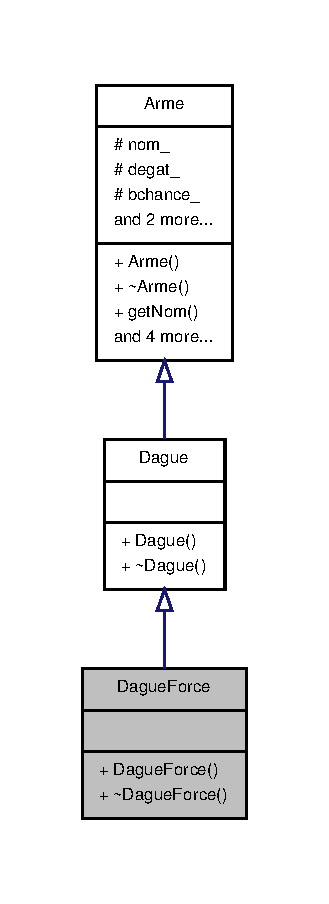
\includegraphics[width=158pt]{class_dague_force__inherit__graph}
\end{center}
\end{figure}


Graphe de collaboration de Dague\-Force\-:
\nopagebreak
\begin{figure}[H]
\begin{center}
\leavevmode
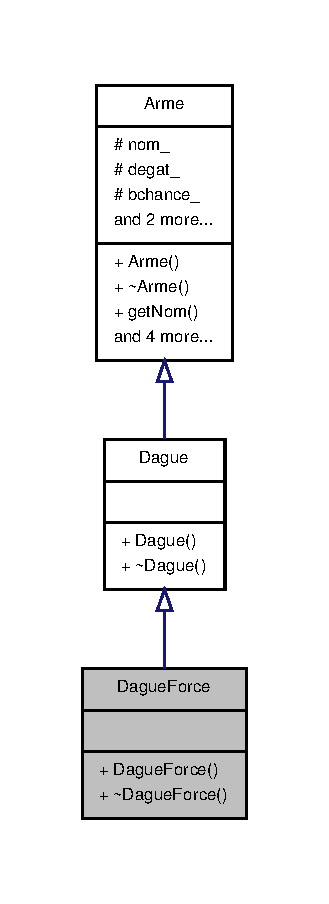
\includegraphics[width=158pt]{class_dague_force__coll__graph}
\end{center}
\end{figure}
\subsection*{Fonctions membres publiques}
\begin{DoxyCompactItemize}
\item 
virtual std\-::string \hyperlink{class_arme_ab1b18cfa41fac19fccedf2165b9ff33c}{get\-Nom} ()
\begin{DoxyCompactList}\small\item\em Retourne le nom de l'arme. \end{DoxyCompactList}\item 
virtual int \hyperlink{class_arme_a3939e914a9ccc898de76db26bc8c24e7}{get\-Bforce} ()
\begin{DoxyCompactList}\small\item\em Retourne le bonus de force. \end{DoxyCompactList}\item 
virtual int \hyperlink{class_arme_a479453fea0d6789e34ccaf193b3098ce}{get\-Bvie} ()
\begin{DoxyCompactList}\small\item\em Retourne le bonus de vie. \end{DoxyCompactList}\item 
virtual int \hyperlink{class_arme_a6cb83d15008174152e424bebd0921069}{get\-Bchance} ()
\begin{DoxyCompactList}\small\item\em Retourne le bonus de chance. \end{DoxyCompactList}\item 
virtual int \hyperlink{class_arme_a06ced3532b0e60cc900674a94c0cf29b}{get\-Degat} ()
\begin{DoxyCompactList}\small\item\em Retourne les degats de l'arme. \end{DoxyCompactList}\end{DoxyCompactItemize}
\subsection*{Attributs protégés}
\begin{DoxyCompactItemize}
\item 
\hypertarget{class_arme_a347394a5ab5c3230259c1b7117f3e8d6}{std\-::string \hyperlink{class_arme_a347394a5ab5c3230259c1b7117f3e8d6}{nom\-\_\-}}\label{class_arme_a347394a5ab5c3230259c1b7117f3e8d6}

\begin{DoxyCompactList}\small\item\em Nom de l'arme. \end{DoxyCompactList}\item 
\hypertarget{class_arme_a15f99a8b95c2d6f5beb9f473df79e399}{int \hyperlink{class_arme_a15f99a8b95c2d6f5beb9f473df79e399}{degat\-\_\-}}\label{class_arme_a15f99a8b95c2d6f5beb9f473df79e399}

\begin{DoxyCompactList}\small\item\em Bonus de dégat. \end{DoxyCompactList}\item 
\hypertarget{class_arme_a688792d4393f9e690aa103a8e68c541c}{int \hyperlink{class_arme_a688792d4393f9e690aa103a8e68c541c}{bchance\-\_\-}}\label{class_arme_a688792d4393f9e690aa103a8e68c541c}

\begin{DoxyCompactList}\small\item\em Bonus de chance. \end{DoxyCompactList}\item 
\hypertarget{class_arme_a4606c075b38ef49f6ed2ed06d6185173}{int \hyperlink{class_arme_a4606c075b38ef49f6ed2ed06d6185173}{bvie\-\_\-}}\label{class_arme_a4606c075b38ef49f6ed2ed06d6185173}

\begin{DoxyCompactList}\small\item\em Bonus de vie. \end{DoxyCompactList}\item 
\hypertarget{class_arme_a779e9838aa9c50d948f58b593fc5954b}{int \hyperlink{class_arme_a779e9838aa9c50d948f58b593fc5954b}{bforce\-\_\-}}\label{class_arme_a779e9838aa9c50d948f58b593fc5954b}

\begin{DoxyCompactList}\small\item\em Bonus de force. \end{DoxyCompactList}\end{DoxyCompactItemize}


\subsection{Description détaillée}
\hyperlink{class_dague_force}{Dague\-Force} herite de \hyperlink{class_dague}{Dague}. 

\subsection{Documentation des fonctions membres}
\hypertarget{class_arme_a6cb83d15008174152e424bebd0921069}{\index{Dague\-Force@{Dague\-Force}!get\-Bchance@{get\-Bchance}}
\index{get\-Bchance@{get\-Bchance}!DagueForce@{Dague\-Force}}
\subsubsection[{get\-Bchance}]{\setlength{\rightskip}{0pt plus 5cm}int Arme\-::get\-Bchance (
\begin{DoxyParamCaption}
{}
\end{DoxyParamCaption}
)\hspace{0.3cm}{\ttfamily [virtual]}, {\ttfamily [inherited]}}}\label{class_arme_a6cb83d15008174152e424bebd0921069}


Retourne le bonus de chance. 

\begin{DoxyReturn}{Renvoie}
Bchance 
\end{DoxyReturn}


Réimplémentée dans \hyperlink{class_d_arme_ad50d376b08d62276b7cf50d2cd59d619}{D\-Arme}.

\hypertarget{class_arme_a3939e914a9ccc898de76db26bc8c24e7}{\index{Dague\-Force@{Dague\-Force}!get\-Bforce@{get\-Bforce}}
\index{get\-Bforce@{get\-Bforce}!DagueForce@{Dague\-Force}}
\subsubsection[{get\-Bforce}]{\setlength{\rightskip}{0pt plus 5cm}int Arme\-::get\-Bforce (
\begin{DoxyParamCaption}
{}
\end{DoxyParamCaption}
)\hspace{0.3cm}{\ttfamily [virtual]}, {\ttfamily [inherited]}}}\label{class_arme_a3939e914a9ccc898de76db26bc8c24e7}


Retourne le bonus de force. 

\begin{DoxyReturn}{Renvoie}
Bforce 
\end{DoxyReturn}


Réimplémentée dans \hyperlink{class_d_arme_a76075bcbe61b20bd0e21e2d06fe33ab7}{D\-Arme}.

\hypertarget{class_arme_a479453fea0d6789e34ccaf193b3098ce}{\index{Dague\-Force@{Dague\-Force}!get\-Bvie@{get\-Bvie}}
\index{get\-Bvie@{get\-Bvie}!DagueForce@{Dague\-Force}}
\subsubsection[{get\-Bvie}]{\setlength{\rightskip}{0pt plus 5cm}int Arme\-::get\-Bvie (
\begin{DoxyParamCaption}
{}
\end{DoxyParamCaption}
)\hspace{0.3cm}{\ttfamily [virtual]}, {\ttfamily [inherited]}}}\label{class_arme_a479453fea0d6789e34ccaf193b3098ce}


Retourne le bonus de vie. 

\begin{DoxyReturn}{Renvoie}
Bvie 
\end{DoxyReturn}


Réimplémentée dans \hyperlink{class_d_arme_a91b3a3100969a568a8408ba098668398}{D\-Arme}.

\hypertarget{class_arme_a06ced3532b0e60cc900674a94c0cf29b}{\index{Dague\-Force@{Dague\-Force}!get\-Degat@{get\-Degat}}
\index{get\-Degat@{get\-Degat}!DagueForce@{Dague\-Force}}
\subsubsection[{get\-Degat}]{\setlength{\rightskip}{0pt plus 5cm}int Arme\-::get\-Degat (
\begin{DoxyParamCaption}
{}
\end{DoxyParamCaption}
)\hspace{0.3cm}{\ttfamily [virtual]}, {\ttfamily [inherited]}}}\label{class_arme_a06ced3532b0e60cc900674a94c0cf29b}


Retourne les degats de l'arme. 

\begin{DoxyReturn}{Renvoie}
degats 
\end{DoxyReturn}


Réimplémentée dans \hyperlink{class_d_arme_a7396e865674067f4f21a28e6babc0fad}{D\-Arme}.

\hypertarget{class_arme_ab1b18cfa41fac19fccedf2165b9ff33c}{\index{Dague\-Force@{Dague\-Force}!get\-Nom@{get\-Nom}}
\index{get\-Nom@{get\-Nom}!DagueForce@{Dague\-Force}}
\subsubsection[{get\-Nom}]{\setlength{\rightskip}{0pt plus 5cm}std\-::string Arme\-::get\-Nom (
\begin{DoxyParamCaption}
{}
\end{DoxyParamCaption}
)\hspace{0.3cm}{\ttfamily [virtual]}, {\ttfamily [inherited]}}}\label{class_arme_ab1b18cfa41fac19fccedf2165b9ff33c}


Retourne le nom de l'arme. 

\begin{DoxyReturn}{Renvoie}
Nom 
\end{DoxyReturn}

\section{Référence de la classe Dague\-Vie}
\label{class_dague_vie}\index{Dague\-Vie@{Dague\-Vie}}


\doxyref{Dague\-Vie}{p.}{class_dague_vie} herite de \doxyref{Dague}{p.}{class_dague}.  




Graphe d'héritage de Dague\-Vie\-:\nopagebreak
\begin{figure}[H]
\begin{center}
\leavevmode
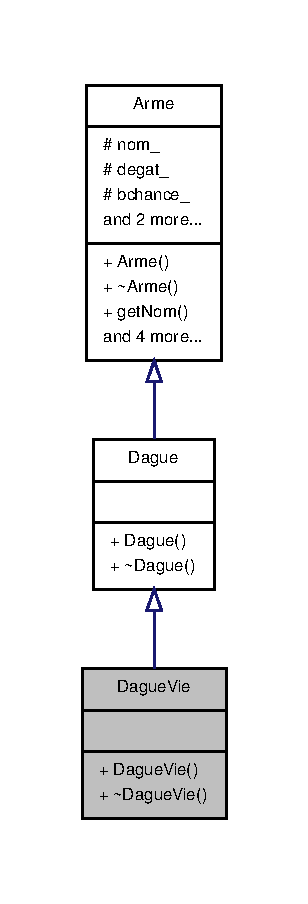
\includegraphics[width=148pt]{class_dague_vie__inherit__graph}
\end{center}
\end{figure}


Graphe de collaboration de Dague\-Vie\-:\nopagebreak
\begin{figure}[H]
\begin{center}
\leavevmode
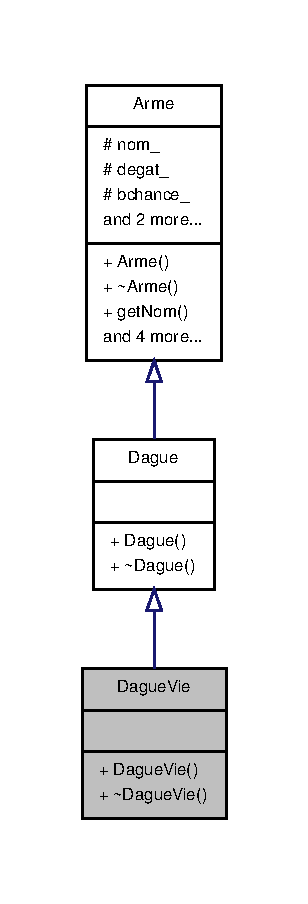
\includegraphics[width=148pt]{class_dague_vie__coll__graph}
\end{center}
\end{figure}
\subsection*{Fonctions membres publiques}
\begin{DoxyCompactItemize}
\item 
{\bf Dague\-Vie} ()
\item 
{\bf $\sim$\-Dague\-Vie} ()
\item 
virtual std\-::string {\bf get\-Nom} ()
\begin{DoxyCompactList}\small\item\em Retourne le nom de l'arme. \end{DoxyCompactList}\item 
virtual int {\bf get\-Bforce} ()
\begin{DoxyCompactList}\small\item\em Retourne le bonus de force. \end{DoxyCompactList}\item 
virtual int {\bf get\-Bvie} ()
\begin{DoxyCompactList}\small\item\em Retourne le bonus de vie. \end{DoxyCompactList}\item 
virtual int {\bf get\-Bchance} ()
\begin{DoxyCompactList}\small\item\em Retourne le bonus de chance. \end{DoxyCompactList}\item 
virtual int {\bf get\-Degat} ()
\begin{DoxyCompactList}\small\item\em Retourne les degats de l'arme. \end{DoxyCompactList}\end{DoxyCompactItemize}
\subsection*{Attributs protégés}
\begin{DoxyCompactItemize}
\item 
std\-::string {\bf nom\-\_\-}
\begin{DoxyCompactList}\small\item\em Nom de l'arme. \end{DoxyCompactList}\item 
int {\bf degat\-\_\-}
\begin{DoxyCompactList}\small\item\em Bonus de dégat. \end{DoxyCompactList}\item 
int {\bf bchance\-\_\-}
\begin{DoxyCompactList}\small\item\em Bonus de chance. \end{DoxyCompactList}\item 
int {\bf bvie\-\_\-}
\begin{DoxyCompactList}\small\item\em Bonus de vie. \end{DoxyCompactList}\item 
int {\bf bforce\-\_\-}
\begin{DoxyCompactList}\small\item\em Bonus de force. \end{DoxyCompactList}\end{DoxyCompactItemize}


\subsection{Description détaillée}
\doxyref{Dague\-Vie}{p.}{class_dague_vie} herite de \doxyref{Dague}{p.}{class_dague}. 

\subsection{Documentation des constructeurs et destructeur}
\index{Dague\-Vie@{Dague\-Vie}!Dague\-Vie@{Dague\-Vie}}
\index{Dague\-Vie@{Dague\-Vie}!DagueVie@{Dague\-Vie}}
\subsubsection[{Dague\-Vie}]{\setlength{\rightskip}{0pt plus 5cm}Dague\-Vie\-::\-Dague\-Vie (
\begin{DoxyParamCaption}
{}
\end{DoxyParamCaption}
)}\label{class_dague_vie_ab7e8a12c2afc29be20e62c836f73659c}
\index{Dague\-Vie@{Dague\-Vie}!$\sim$\-Dague\-Vie@{$\sim$\-Dague\-Vie}}
\index{$\sim$\-Dague\-Vie@{$\sim$\-Dague\-Vie}!DagueVie@{Dague\-Vie}}
\subsubsection[{$\sim$\-Dague\-Vie}]{\setlength{\rightskip}{0pt plus 5cm}Dague\-Vie\-::$\sim$\-Dague\-Vie (
\begin{DoxyParamCaption}
{}
\end{DoxyParamCaption}
)}\label{class_dague_vie_aebae77004857b8da4caf9a07c9465e43}


\subsection{Documentation des fonctions membres}
\index{Dague\-Vie@{Dague\-Vie}!get\-Bchance@{get\-Bchance}}
\index{get\-Bchance@{get\-Bchance}!DagueVie@{Dague\-Vie}}
\subsubsection[{get\-Bchance}]{\setlength{\rightskip}{0pt plus 5cm}int Arme\-::get\-Bchance (
\begin{DoxyParamCaption}
{}
\end{DoxyParamCaption}
)\hspace{0.3cm}{\ttfamily [virtual]}, {\ttfamily [inherited]}}\label{class_arme_a6cb83d15008174152e424bebd0921069}


Retourne le bonus de chance. 

\begin{DoxyReturn}{Renvoie}
Bchance 
\end{DoxyReturn}


Réimplémentée dans {\bf D\-Arme} \doxyref{}{p.}{class_d_arme_ad50d376b08d62276b7cf50d2cd59d619}.

\index{Dague\-Vie@{Dague\-Vie}!get\-Bforce@{get\-Bforce}}
\index{get\-Bforce@{get\-Bforce}!DagueVie@{Dague\-Vie}}
\subsubsection[{get\-Bforce}]{\setlength{\rightskip}{0pt plus 5cm}int Arme\-::get\-Bforce (
\begin{DoxyParamCaption}
{}
\end{DoxyParamCaption}
)\hspace{0.3cm}{\ttfamily [virtual]}, {\ttfamily [inherited]}}\label{class_arme_a3939e914a9ccc898de76db26bc8c24e7}


Retourne le bonus de force. 

\begin{DoxyReturn}{Renvoie}
Bforce 
\end{DoxyReturn}


Réimplémentée dans {\bf D\-Arme} \doxyref{}{p.}{class_d_arme_a76075bcbe61b20bd0e21e2d06fe33ab7}.

\index{Dague\-Vie@{Dague\-Vie}!get\-Bvie@{get\-Bvie}}
\index{get\-Bvie@{get\-Bvie}!DagueVie@{Dague\-Vie}}
\subsubsection[{get\-Bvie}]{\setlength{\rightskip}{0pt plus 5cm}int Arme\-::get\-Bvie (
\begin{DoxyParamCaption}
{}
\end{DoxyParamCaption}
)\hspace{0.3cm}{\ttfamily [virtual]}, {\ttfamily [inherited]}}\label{class_arme_a479453fea0d6789e34ccaf193b3098ce}


Retourne le bonus de vie. 

\begin{DoxyReturn}{Renvoie}
Bvie 
\end{DoxyReturn}


Réimplémentée dans {\bf D\-Arme} \doxyref{}{p.}{class_d_arme_a91b3a3100969a568a8408ba098668398}.

\index{Dague\-Vie@{Dague\-Vie}!get\-Degat@{get\-Degat}}
\index{get\-Degat@{get\-Degat}!DagueVie@{Dague\-Vie}}
\subsubsection[{get\-Degat}]{\setlength{\rightskip}{0pt plus 5cm}int Arme\-::get\-Degat (
\begin{DoxyParamCaption}
{}
\end{DoxyParamCaption}
)\hspace{0.3cm}{\ttfamily [virtual]}, {\ttfamily [inherited]}}\label{class_arme_a06ced3532b0e60cc900674a94c0cf29b}


Retourne les degats de l'arme. 

\begin{DoxyReturn}{Renvoie}
degats 
\end{DoxyReturn}


Réimplémentée dans {\bf D\-Arme} \doxyref{}{p.}{class_d_arme_a7396e865674067f4f21a28e6babc0fad}.

\index{Dague\-Vie@{Dague\-Vie}!get\-Nom@{get\-Nom}}
\index{get\-Nom@{get\-Nom}!DagueVie@{Dague\-Vie}}
\subsubsection[{get\-Nom}]{\setlength{\rightskip}{0pt plus 5cm}std\-::string Arme\-::get\-Nom (
\begin{DoxyParamCaption}
{}
\end{DoxyParamCaption}
)\hspace{0.3cm}{\ttfamily [virtual]}, {\ttfamily [inherited]}}\label{class_arme_ab1b18cfa41fac19fccedf2165b9ff33c}


Retourne le nom de l'arme. 

\begin{DoxyReturn}{Renvoie}
Nom 
\end{DoxyReturn}


\subsection{Documentation des données membres}
\index{Dague\-Vie@{Dague\-Vie}!bchance\-\_\-@{bchance\-\_\-}}
\index{bchance\-\_\-@{bchance\-\_\-}!DagueVie@{Dague\-Vie}}
\subsubsection[{bchance\-\_\-}]{\setlength{\rightskip}{0pt plus 5cm}int Arme\-::bchance\-\_\-\hspace{0.3cm}{\ttfamily [protected]}, {\ttfamily [inherited]}}\label{class_arme_a688792d4393f9e690aa103a8e68c541c}


Bonus de chance. 

\index{Dague\-Vie@{Dague\-Vie}!bforce\-\_\-@{bforce\-\_\-}}
\index{bforce\-\_\-@{bforce\-\_\-}!DagueVie@{Dague\-Vie}}
\subsubsection[{bforce\-\_\-}]{\setlength{\rightskip}{0pt plus 5cm}int Arme\-::bforce\-\_\-\hspace{0.3cm}{\ttfamily [protected]}, {\ttfamily [inherited]}}\label{class_arme_a779e9838aa9c50d948f58b593fc5954b}


Bonus de force. 

\index{Dague\-Vie@{Dague\-Vie}!bvie\-\_\-@{bvie\-\_\-}}
\index{bvie\-\_\-@{bvie\-\_\-}!DagueVie@{Dague\-Vie}}
\subsubsection[{bvie\-\_\-}]{\setlength{\rightskip}{0pt plus 5cm}int Arme\-::bvie\-\_\-\hspace{0.3cm}{\ttfamily [protected]}, {\ttfamily [inherited]}}\label{class_arme_a4606c075b38ef49f6ed2ed06d6185173}


Bonus de vie. 

\index{Dague\-Vie@{Dague\-Vie}!degat\-\_\-@{degat\-\_\-}}
\index{degat\-\_\-@{degat\-\_\-}!DagueVie@{Dague\-Vie}}
\subsubsection[{degat\-\_\-}]{\setlength{\rightskip}{0pt plus 5cm}int Arme\-::degat\-\_\-\hspace{0.3cm}{\ttfamily [protected]}, {\ttfamily [inherited]}}\label{class_arme_a15f99a8b95c2d6f5beb9f473df79e399}


Bonus de dégat. 

\index{Dague\-Vie@{Dague\-Vie}!nom\-\_\-@{nom\-\_\-}}
\index{nom\-\_\-@{nom\-\_\-}!DagueVie@{Dague\-Vie}}
\subsubsection[{nom\-\_\-}]{\setlength{\rightskip}{0pt plus 5cm}std\-::string Arme\-::nom\-\_\-\hspace{0.3cm}{\ttfamily [protected]}, {\ttfamily [inherited]}}\label{class_arme_a347394a5ab5c3230259c1b7117f3e8d6}


Nom de l'arme. 



La documentation de cette classe a été générée à partir des fichiers suivants \-:\begin{DoxyCompactItemize}
\item 
src/{\bf Dague\-Vie.\-hpp}\item 
src/{\bf Dague\-Vie.\-cpp}\end{DoxyCompactItemize}

\section{Référence de la classe D\-Arme}
\label{class_d_arme}\index{D\-Arme@{D\-Arme}}


Decorator d'arme, hérite de \doxyref{Arme}{p.}{class_arme}.  




Graphe d'héritage de D\-Arme\-:\nopagebreak
\begin{figure}[H]
\begin{center}
\leavevmode
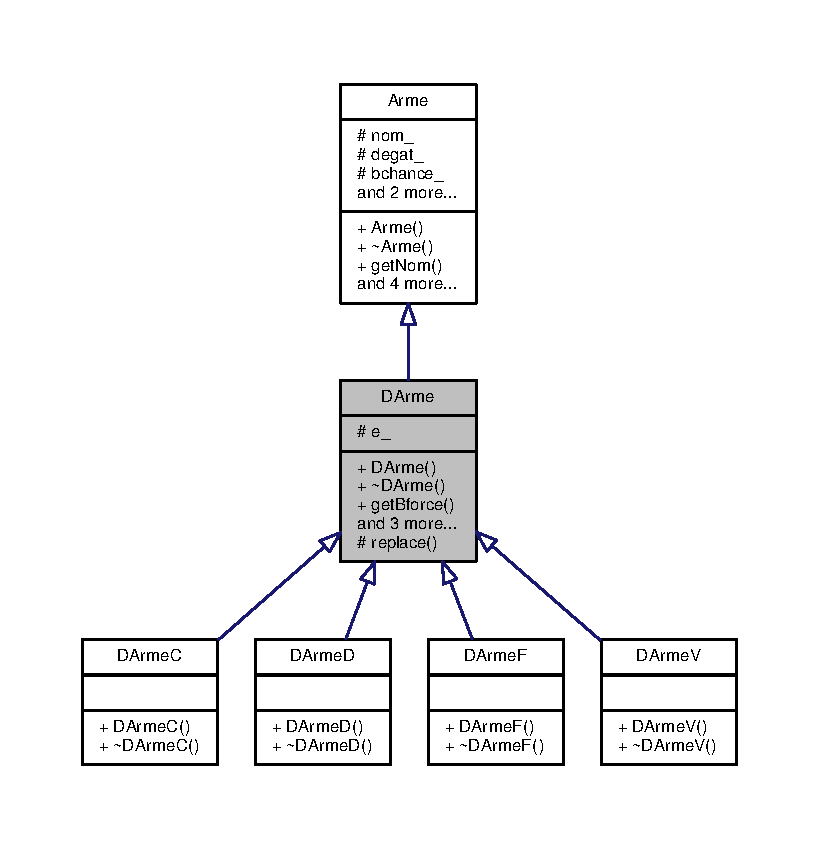
\includegraphics[width=350pt]{class_d_arme__inherit__graph}
\end{center}
\end{figure}


Graphe de collaboration de D\-Arme\-:\nopagebreak
\begin{figure}[H]
\begin{center}
\leavevmode
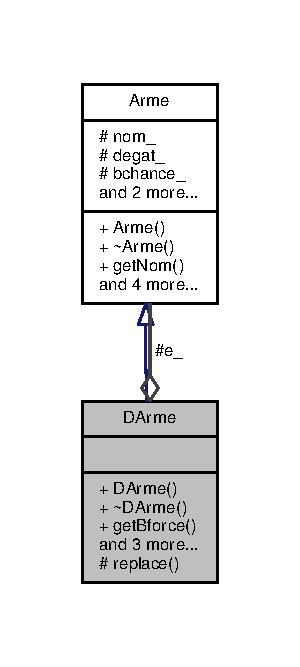
\includegraphics[width=144pt]{class_d_arme__coll__graph}
\end{center}
\end{figure}
\subsection*{Fonctions membres publiques}
\begin{DoxyCompactItemize}
\item 
{\bf D\-Arme} ({\bf Arme} $\ast$e)
\begin{DoxyCompactList}\small\item\em Constructeur du Decorator d'arme. \end{DoxyCompactList}\item 
virtual {\bf $\sim$\-D\-Arme} ()
\item 
int {\bf get\-Bforce} ()
\begin{DoxyCompactList}\small\item\em Renvoie le bonus de force. \end{DoxyCompactList}\item 
int {\bf get\-Bvie} ()
\begin{DoxyCompactList}\small\item\em Renvoie le bonus de vie. \end{DoxyCompactList}\item 
int {\bf get\-Bchance} ()
\begin{DoxyCompactList}\small\item\em Renvoie le bonus de chance. \end{DoxyCompactList}\item 
int {\bf get\-Degat} ()
\begin{DoxyCompactList}\small\item\em Renvoie les dégâts. \end{DoxyCompactList}\item 
virtual std\-::string {\bf get\-Nom} ()
\begin{DoxyCompactList}\small\item\em Retourne le nom de l'arme. \end{DoxyCompactList}\end{DoxyCompactItemize}
\subsection*{Fonctions membres protégées}
\begin{DoxyCompactItemize}
\item 
std\-::string {\bf replace} (std\-::string str)
\begin{DoxyCompactList}\small\item\em Retourne le nom de l'arme modifié \end{DoxyCompactList}\end{DoxyCompactItemize}
\subsection*{Attributs protégés}
\begin{DoxyCompactItemize}
\item 
{\bf Arme} $\ast$ {\bf e\-\_\-}
\begin{DoxyCompactList}\small\item\em \doxyref{Arme}{p.}{class_arme} pour les decorations. \end{DoxyCompactList}\item 
std\-::string {\bf nom\-\_\-}
\begin{DoxyCompactList}\small\item\em Nom de l'arme. \end{DoxyCompactList}\item 
int {\bf degat\-\_\-}
\begin{DoxyCompactList}\small\item\em Bonus de dégat. \end{DoxyCompactList}\item 
int {\bf bchance\-\_\-}
\begin{DoxyCompactList}\small\item\em Bonus de chance. \end{DoxyCompactList}\item 
int {\bf bvie\-\_\-}
\begin{DoxyCompactList}\small\item\em Bonus de vie. \end{DoxyCompactList}\item 
int {\bf bforce\-\_\-}
\begin{DoxyCompactList}\small\item\em Bonus de force. \end{DoxyCompactList}\end{DoxyCompactItemize}


\subsection{Description détaillée}
Decorator d'arme, hérite de \doxyref{Arme}{p.}{class_arme}. 

\subsection{Documentation des constructeurs et destructeur}
\index{D\-Arme@{D\-Arme}!D\-Arme@{D\-Arme}}
\index{D\-Arme@{D\-Arme}!DArme@{D\-Arme}}
\subsubsection[{D\-Arme}]{\setlength{\rightskip}{0pt plus 5cm}D\-Arme\-::\-D\-Arme (
\begin{DoxyParamCaption}
\item[{{\bf Arme} $\ast$}]{e}
\end{DoxyParamCaption}
)}\label{class_d_arme_adb0f0f90c314d30362d9a31a53173a70}


Constructeur du Decorator d'arme. 

\index{D\-Arme@{D\-Arme}!$\sim$\-D\-Arme@{$\sim$\-D\-Arme}}
\index{$\sim$\-D\-Arme@{$\sim$\-D\-Arme}!DArme@{D\-Arme}}
\subsubsection[{$\sim$\-D\-Arme}]{\setlength{\rightskip}{0pt plus 5cm}D\-Arme\-::$\sim$\-D\-Arme (
\begin{DoxyParamCaption}
{}
\end{DoxyParamCaption}
)\hspace{0.3cm}{\ttfamily [virtual]}}\label{class_d_arme_ab1215e07fcd942a3d06bbc5fe0f4083c}


\subsection{Documentation des fonctions membres}
\index{D\-Arme@{D\-Arme}!get\-Bchance@{get\-Bchance}}
\index{get\-Bchance@{get\-Bchance}!DArme@{D\-Arme}}
\subsubsection[{get\-Bchance}]{\setlength{\rightskip}{0pt plus 5cm}int D\-Arme\-::get\-Bchance (
\begin{DoxyParamCaption}
{}
\end{DoxyParamCaption}
)\hspace{0.3cm}{\ttfamily [virtual]}}\label{class_d_arme_ad50d376b08d62276b7cf50d2cd59d619}


Renvoie le bonus de chance. 

\begin{DoxyReturn}{Renvoie}
bchance Bonus de chance 
\end{DoxyReturn}


Réimplémentée à partir de {\bf Arme} \doxyref{}{p.}{class_arme_a6cb83d15008174152e424bebd0921069}.

\index{D\-Arme@{D\-Arme}!get\-Bforce@{get\-Bforce}}
\index{get\-Bforce@{get\-Bforce}!DArme@{D\-Arme}}
\subsubsection[{get\-Bforce}]{\setlength{\rightskip}{0pt plus 5cm}int D\-Arme\-::get\-Bforce (
\begin{DoxyParamCaption}
{}
\end{DoxyParamCaption}
)\hspace{0.3cm}{\ttfamily [virtual]}}\label{class_d_arme_a76075bcbe61b20bd0e21e2d06fe33ab7}


Renvoie le bonus de force. 

\begin{DoxyReturn}{Renvoie}
bforce Bonus de force 
\end{DoxyReturn}


Réimplémentée à partir de {\bf Arme} \doxyref{}{p.}{class_arme_a3939e914a9ccc898de76db26bc8c24e7}.

\index{D\-Arme@{D\-Arme}!get\-Bvie@{get\-Bvie}}
\index{get\-Bvie@{get\-Bvie}!DArme@{D\-Arme}}
\subsubsection[{get\-Bvie}]{\setlength{\rightskip}{0pt plus 5cm}int D\-Arme\-::get\-Bvie (
\begin{DoxyParamCaption}
{}
\end{DoxyParamCaption}
)\hspace{0.3cm}{\ttfamily [virtual]}}\label{class_d_arme_a91b3a3100969a568a8408ba098668398}


Renvoie le bonus de vie. 

\begin{DoxyReturn}{Renvoie}
bvie Bonus de vie 
\end{DoxyReturn}


Réimplémentée à partir de {\bf Arme} \doxyref{}{p.}{class_arme_a479453fea0d6789e34ccaf193b3098ce}.

\index{D\-Arme@{D\-Arme}!get\-Degat@{get\-Degat}}
\index{get\-Degat@{get\-Degat}!DArme@{D\-Arme}}
\subsubsection[{get\-Degat}]{\setlength{\rightskip}{0pt plus 5cm}int D\-Arme\-::get\-Degat (
\begin{DoxyParamCaption}
{}
\end{DoxyParamCaption}
)\hspace{0.3cm}{\ttfamily [virtual]}}\label{class_d_arme_a7396e865674067f4f21a28e6babc0fad}


Renvoie les dégâts. 

\begin{DoxyReturn}{Renvoie}
degat Dégâts 
\end{DoxyReturn}


Réimplémentée à partir de {\bf Arme} \doxyref{}{p.}{class_arme_a06ced3532b0e60cc900674a94c0cf29b}.

\index{D\-Arme@{D\-Arme}!get\-Nom@{get\-Nom}}
\index{get\-Nom@{get\-Nom}!DArme@{D\-Arme}}
\subsubsection[{get\-Nom}]{\setlength{\rightskip}{0pt plus 5cm}std\-::string Arme\-::get\-Nom (
\begin{DoxyParamCaption}
{}
\end{DoxyParamCaption}
)\hspace{0.3cm}{\ttfamily [virtual]}, {\ttfamily [inherited]}}\label{class_arme_ab1b18cfa41fac19fccedf2165b9ff33c}


Retourne le nom de l'arme. 

\begin{DoxyReturn}{Renvoie}
Nom 
\end{DoxyReturn}
\index{D\-Arme@{D\-Arme}!replace@{replace}}
\index{replace@{replace}!DArme@{D\-Arme}}
\subsubsection[{replace}]{\setlength{\rightskip}{0pt plus 5cm}std\-::string D\-Arme\-::replace (
\begin{DoxyParamCaption}
\item[{std\-::string}]{str}
\end{DoxyParamCaption}
)\hspace{0.3cm}{\ttfamily [protected]}}\label{class_d_arme_a604caa7ee656dab58d15b7cf86863e3d}


Retourne le nom de l'arme modifié 


\begin{DoxyParams}{Paramètres}
{\em Chaine} & de caractère à ajouter \\
\hline
\end{DoxyParams}
\begin{DoxyReturn}{Renvoie}
nom nom modifié 
\end{DoxyReturn}


\subsection{Documentation des données membres}
\index{D\-Arme@{D\-Arme}!bchance\-\_\-@{bchance\-\_\-}}
\index{bchance\-\_\-@{bchance\-\_\-}!DArme@{D\-Arme}}
\subsubsection[{bchance\-\_\-}]{\setlength{\rightskip}{0pt plus 5cm}int Arme\-::bchance\-\_\-\hspace{0.3cm}{\ttfamily [protected]}, {\ttfamily [inherited]}}\label{class_arme_a688792d4393f9e690aa103a8e68c541c}


Bonus de chance. 

\index{D\-Arme@{D\-Arme}!bforce\-\_\-@{bforce\-\_\-}}
\index{bforce\-\_\-@{bforce\-\_\-}!DArme@{D\-Arme}}
\subsubsection[{bforce\-\_\-}]{\setlength{\rightskip}{0pt plus 5cm}int Arme\-::bforce\-\_\-\hspace{0.3cm}{\ttfamily [protected]}, {\ttfamily [inherited]}}\label{class_arme_a779e9838aa9c50d948f58b593fc5954b}


Bonus de force. 

\index{D\-Arme@{D\-Arme}!bvie\-\_\-@{bvie\-\_\-}}
\index{bvie\-\_\-@{bvie\-\_\-}!DArme@{D\-Arme}}
\subsubsection[{bvie\-\_\-}]{\setlength{\rightskip}{0pt plus 5cm}int Arme\-::bvie\-\_\-\hspace{0.3cm}{\ttfamily [protected]}, {\ttfamily [inherited]}}\label{class_arme_a4606c075b38ef49f6ed2ed06d6185173}


Bonus de vie. 

\index{D\-Arme@{D\-Arme}!degat\-\_\-@{degat\-\_\-}}
\index{degat\-\_\-@{degat\-\_\-}!DArme@{D\-Arme}}
\subsubsection[{degat\-\_\-}]{\setlength{\rightskip}{0pt plus 5cm}int Arme\-::degat\-\_\-\hspace{0.3cm}{\ttfamily [protected]}, {\ttfamily [inherited]}}\label{class_arme_a15f99a8b95c2d6f5beb9f473df79e399}


Bonus de dégat. 

\index{D\-Arme@{D\-Arme}!e\-\_\-@{e\-\_\-}}
\index{e\-\_\-@{e\-\_\-}!DArme@{D\-Arme}}
\subsubsection[{e\-\_\-}]{\setlength{\rightskip}{0pt plus 5cm}{\bf Arme}$\ast$ D\-Arme\-::e\-\_\-\hspace{0.3cm}{\ttfamily [protected]}}\label{class_d_arme_a03856c36a22fe5bb49f6479d0b864df2}


\doxyref{Arme}{p.}{class_arme} pour les decorations. 

\index{D\-Arme@{D\-Arme}!nom\-\_\-@{nom\-\_\-}}
\index{nom\-\_\-@{nom\-\_\-}!DArme@{D\-Arme}}
\subsubsection[{nom\-\_\-}]{\setlength{\rightskip}{0pt plus 5cm}std\-::string Arme\-::nom\-\_\-\hspace{0.3cm}{\ttfamily [protected]}, {\ttfamily [inherited]}}\label{class_arme_a347394a5ab5c3230259c1b7117f3e8d6}


Nom de l'arme. 



La documentation de cette classe a été générée à partir des fichiers suivants \-:\begin{DoxyCompactItemize}
\item 
src/{\bf D\-Arme.\-hpp}\item 
src/{\bf D\-Arme.\-cpp}\end{DoxyCompactItemize}

\section{Référence de la classe D\-Arme\-C}
\label{class_d_arme_c}\index{D\-Arme\-C@{D\-Arme\-C}}


Graphe d'héritage de D\-Arme\-C\-:\nopagebreak
\begin{figure}[H]
\begin{center}
\leavevmode
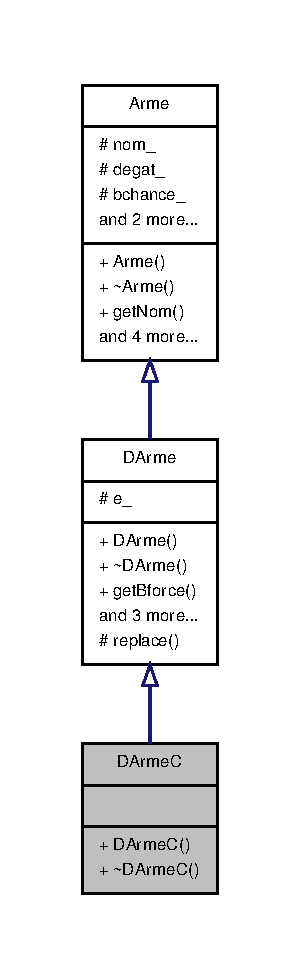
\includegraphics[width=144pt]{class_d_arme_c__inherit__graph}
\end{center}
\end{figure}


Graphe de collaboration de D\-Arme\-C\-:\nopagebreak
\begin{figure}[H]
\begin{center}
\leavevmode
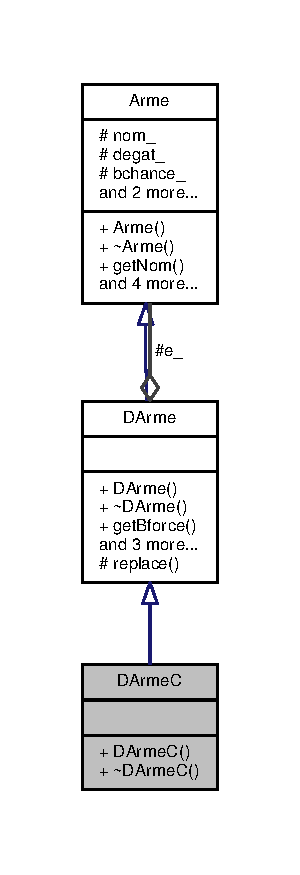
\includegraphics[width=144pt]{class_d_arme_c__coll__graph}
\end{center}
\end{figure}
\subsection*{Fonctions membres publiques}
\begin{DoxyCompactItemize}
\item 
{\bf D\-Arme\-C} ({\bf Arme} $\ast$e)
\item 
{\bf $\sim$\-D\-Arme\-C} ()
\item 
std\-::string {\bf get\-Nom} ()
\item 
int {\bf get\-Bforce} ()
\item 
int {\bf get\-Bvie} ()
\item 
int {\bf get\-Bchance} ()
\item 
int {\bf get\-Degat} ()
\item 
void {\bf set\-Bforce} (int bforce)
\item 
void {\bf set\-Bvie} (int bvie)
\item 
void {\bf set\-Bchance} (int bchance)
\item 
void {\bf set\-Degat} (int degat)
\item 
void {\bf set\-Nom} (std\-::string nom)
\end{DoxyCompactItemize}
\subsection*{Attributs privés}
\begin{DoxyCompactItemize}
\item 
{\bf Arme} $\ast$ {\bf e\-\_\-}
\end{DoxyCompactItemize}


\subsection{Documentation des constructeurs et destructeur}
\index{D\-Arme\-C@{D\-Arme\-C}!D\-Arme\-C@{D\-Arme\-C}}
\index{D\-Arme\-C@{D\-Arme\-C}!DArmeC@{D\-Arme\-C}}
\subsubsection[{D\-Arme\-C}]{\setlength{\rightskip}{0pt plus 5cm}D\-Arme\-C\-::\-D\-Arme\-C (
\begin{DoxyParamCaption}
\item[{{\bf Arme} $\ast$}]{e}
\end{DoxyParamCaption}
)}\label{class_d_arme_c_a955ace5c3e5610479dedc8fd9511c77e}
\index{D\-Arme\-C@{D\-Arme\-C}!$\sim$\-D\-Arme\-C@{$\sim$\-D\-Arme\-C}}
\index{$\sim$\-D\-Arme\-C@{$\sim$\-D\-Arme\-C}!DArmeC@{D\-Arme\-C}}
\subsubsection[{$\sim$\-D\-Arme\-C}]{\setlength{\rightskip}{0pt plus 5cm}D\-Arme\-C\-::$\sim$\-D\-Arme\-C (
\begin{DoxyParamCaption}
{}
\end{DoxyParamCaption}
)}\label{class_d_arme_c_a74bd85082699a5d3b534efcdcd8bb096}


\subsection{Documentation des fonctions membres}
\index{D\-Arme\-C@{D\-Arme\-C}!get\-Bchance@{get\-Bchance}}
\index{get\-Bchance@{get\-Bchance}!DArmeC@{D\-Arme\-C}}
\subsubsection[{get\-Bchance}]{\setlength{\rightskip}{0pt plus 5cm}int D\-Arme\-C\-::get\-Bchance (
\begin{DoxyParamCaption}
{}
\end{DoxyParamCaption}
)\hspace{0.3cm}{\ttfamily [virtual]}}\label{class_d_arme_c_a33d7e704e737bdaa81a038dc6753c4c9}


Implémente {\bf Arme} \doxyref{}{p.}{class_arme_afcd4a79f4603cd9ced1eafd15be54316}.

\index{D\-Arme\-C@{D\-Arme\-C}!get\-Bforce@{get\-Bforce}}
\index{get\-Bforce@{get\-Bforce}!DArmeC@{D\-Arme\-C}}
\subsubsection[{get\-Bforce}]{\setlength{\rightskip}{0pt plus 5cm}int D\-Arme\-C\-::get\-Bforce (
\begin{DoxyParamCaption}
{}
\end{DoxyParamCaption}
)\hspace{0.3cm}{\ttfamily [virtual]}}\label{class_d_arme_c_a8897906b826ed33f3a1af20b7ee7b21c}


Implémente {\bf Arme} \doxyref{}{p.}{class_arme_a25da1859e12ebceb90283fb980f00758}.

\index{D\-Arme\-C@{D\-Arme\-C}!get\-Bvie@{get\-Bvie}}
\index{get\-Bvie@{get\-Bvie}!DArmeC@{D\-Arme\-C}}
\subsubsection[{get\-Bvie}]{\setlength{\rightskip}{0pt plus 5cm}int D\-Arme\-C\-::get\-Bvie (
\begin{DoxyParamCaption}
{}
\end{DoxyParamCaption}
)\hspace{0.3cm}{\ttfamily [virtual]}}\label{class_d_arme_c_aac29897179bf6d6b3d98b68333097736}


Implémente {\bf Arme} \doxyref{}{p.}{class_arme_ad07794203a8fa685391cd6c107529aa1}.

\index{D\-Arme\-C@{D\-Arme\-C}!get\-Degat@{get\-Degat}}
\index{get\-Degat@{get\-Degat}!DArmeC@{D\-Arme\-C}}
\subsubsection[{get\-Degat}]{\setlength{\rightskip}{0pt plus 5cm}int D\-Arme\-C\-::get\-Degat (
\begin{DoxyParamCaption}
{}
\end{DoxyParamCaption}
)\hspace{0.3cm}{\ttfamily [virtual]}}\label{class_d_arme_c_a3819d78ab37fd6fae45bb03eb15fc03a}


Implémente {\bf Arme} \doxyref{}{p.}{class_arme_a93e1b6f8c800359c7651b2fc456a3ee1}.

\index{D\-Arme\-C@{D\-Arme\-C}!get\-Nom@{get\-Nom}}
\index{get\-Nom@{get\-Nom}!DArmeC@{D\-Arme\-C}}
\subsubsection[{get\-Nom}]{\setlength{\rightskip}{0pt plus 5cm}std\-::string D\-Arme\-C\-::get\-Nom (
\begin{DoxyParamCaption}
{}
\end{DoxyParamCaption}
)\hspace{0.3cm}{\ttfamily [virtual]}}\label{class_d_arme_c_ac7553787a322cc23a8d1500b1e12f3cd}


Implémente {\bf Arme} \doxyref{}{p.}{class_arme_a0b6a30975be57770c6cae357b52395a0}.

\index{D\-Arme\-C@{D\-Arme\-C}!set\-Bchance@{set\-Bchance}}
\index{set\-Bchance@{set\-Bchance}!DArmeC@{D\-Arme\-C}}
\subsubsection[{set\-Bchance}]{\setlength{\rightskip}{0pt plus 5cm}void D\-Arme\-C\-::set\-Bchance (
\begin{DoxyParamCaption}
\item[{int}]{bchance}
\end{DoxyParamCaption}
)\hspace{0.3cm}{\ttfamily [virtual]}}\label{class_d_arme_c_a636d1d22f4769fc1a6f89125dd58f5c9}


Implémente {\bf Arme} \doxyref{}{p.}{class_arme_a27aa7d294d01ea38975841ea680a815a}.

\index{D\-Arme\-C@{D\-Arme\-C}!set\-Bforce@{set\-Bforce}}
\index{set\-Bforce@{set\-Bforce}!DArmeC@{D\-Arme\-C}}
\subsubsection[{set\-Bforce}]{\setlength{\rightskip}{0pt plus 5cm}void D\-Arme\-C\-::set\-Bforce (
\begin{DoxyParamCaption}
\item[{int}]{bforce}
\end{DoxyParamCaption}
)\hspace{0.3cm}{\ttfamily [virtual]}}\label{class_d_arme_c_a9ce567806ba4e74c55753cfb1080a08d}


Implémente {\bf Arme} \doxyref{}{p.}{class_arme_a8806ba4300d435ebe71bb4b9829296e8}.

\index{D\-Arme\-C@{D\-Arme\-C}!set\-Bvie@{set\-Bvie}}
\index{set\-Bvie@{set\-Bvie}!DArmeC@{D\-Arme\-C}}
\subsubsection[{set\-Bvie}]{\setlength{\rightskip}{0pt plus 5cm}void D\-Arme\-C\-::set\-Bvie (
\begin{DoxyParamCaption}
\item[{int}]{bvie}
\end{DoxyParamCaption}
)\hspace{0.3cm}{\ttfamily [virtual]}}\label{class_d_arme_c_a758cea41196bcb19552d72955ec04735}


Implémente {\bf Arme} \doxyref{}{p.}{class_arme_a0580ea53e4254942a4ef82aec8706ead}.

\index{D\-Arme\-C@{D\-Arme\-C}!set\-Degat@{set\-Degat}}
\index{set\-Degat@{set\-Degat}!DArmeC@{D\-Arme\-C}}
\subsubsection[{set\-Degat}]{\setlength{\rightskip}{0pt plus 5cm}void D\-Arme\-C\-::set\-Degat (
\begin{DoxyParamCaption}
\item[{int}]{degat}
\end{DoxyParamCaption}
)\hspace{0.3cm}{\ttfamily [virtual]}}\label{class_d_arme_c_a80521baa4e17c25587c5131be58a6f7a}


Implémente {\bf Arme} \doxyref{}{p.}{class_arme_a2e2cd008885e4ba4dca346905e7e5f73}.

\index{D\-Arme\-C@{D\-Arme\-C}!set\-Nom@{set\-Nom}}
\index{set\-Nom@{set\-Nom}!DArmeC@{D\-Arme\-C}}
\subsubsection[{set\-Nom}]{\setlength{\rightskip}{0pt plus 5cm}void D\-Arme\-C\-::set\-Nom (
\begin{DoxyParamCaption}
\item[{std\-::string}]{nom}
\end{DoxyParamCaption}
)\hspace{0.3cm}{\ttfamily [virtual]}}\label{class_d_arme_c_aad343bffc110d37e041d0bfc00f632a0}


Implémente {\bf Arme} \doxyref{}{p.}{class_arme_a561f12b90bd01d26328541ba54f6aaa6}.



\subsection{Documentation des données membres}
\index{D\-Arme\-C@{D\-Arme\-C}!e\-\_\-@{e\-\_\-}}
\index{e\-\_\-@{e\-\_\-}!DArmeC@{D\-Arme\-C}}
\subsubsection[{e\-\_\-}]{\setlength{\rightskip}{0pt plus 5cm}{\bf Arme}$\ast$ D\-Arme\-C\-::e\-\_\-\hspace{0.3cm}{\ttfamily [private]}}\label{class_d_arme_c_aeb33234a3cd67598cb54f93c7ad2ef6d}


La documentation de cette classe a été générée à partir du fichier suivant \-:\begin{DoxyCompactItemize}
\item 
src/{\bf D\-Arme\-C.\-hpp}\end{DoxyCompactItemize}

\hypertarget{class_d_arme_d}{\section{Référence de la classe D\-Arme\-D}
\label{class_d_arme_d}\index{D\-Arme\-D@{D\-Arme\-D}}
}


Decorator d'arme de degats, hérite de \hyperlink{class_d_arme}{D\-Arme}.  




Graphe d'héritage de D\-Arme\-D\-:
\nopagebreak
\begin{figure}[H]
\begin{center}
\leavevmode
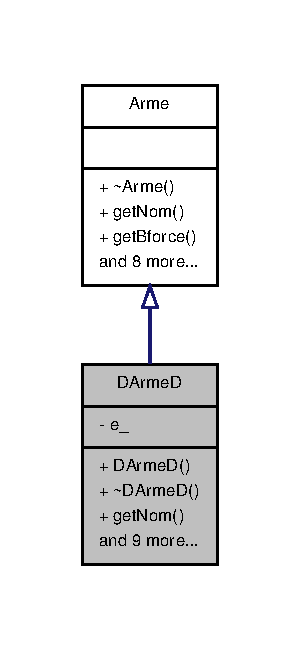
\includegraphics[width=144pt]{class_d_arme_d__inherit__graph}
\end{center}
\end{figure}


Graphe de collaboration de D\-Arme\-D\-:
\nopagebreak
\begin{figure}[H]
\begin{center}
\leavevmode
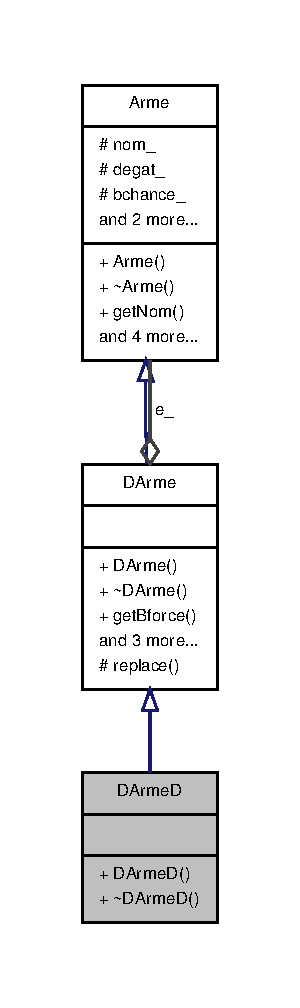
\includegraphics[width=144pt]{class_d_arme_d__coll__graph}
\end{center}
\end{figure}
\subsection*{Fonctions membres publiques}
\begin{DoxyCompactItemize}
\item 
\hypertarget{class_d_arme_d_ad486d2bfb8bd3d4657a1b09a85eb6865}{{\bfseries D\-Arme\-D} (\hyperlink{class_arme}{Arme} $\ast$e)}\label{class_d_arme_d_ad486d2bfb8bd3d4657a1b09a85eb6865}

\item 
int \hyperlink{class_d_arme_a76075bcbe61b20bd0e21e2d06fe33ab7}{get\-Bforce} ()
\begin{DoxyCompactList}\small\item\em Renvoie le bonus de force. \end{DoxyCompactList}\item 
int \hyperlink{class_d_arme_a91b3a3100969a568a8408ba098668398}{get\-Bvie} ()
\begin{DoxyCompactList}\small\item\em Renvoie le bonus de vie. \end{DoxyCompactList}\item 
int \hyperlink{class_d_arme_ad50d376b08d62276b7cf50d2cd59d619}{get\-Bchance} ()
\begin{DoxyCompactList}\small\item\em Renvoie le bonus de chance. \end{DoxyCompactList}\item 
int \hyperlink{class_d_arme_a7396e865674067f4f21a28e6babc0fad}{get\-Degat} ()
\begin{DoxyCompactList}\small\item\em Renvoie les dégâts. \end{DoxyCompactList}\item 
virtual std\-::string \hyperlink{class_arme_ab1b18cfa41fac19fccedf2165b9ff33c}{get\-Nom} ()
\begin{DoxyCompactList}\small\item\em Retourne le nom de l'arme. \end{DoxyCompactList}\end{DoxyCompactItemize}
\subsection*{Fonctions membres protégées}
\begin{DoxyCompactItemize}
\item 
std\-::string \hyperlink{class_d_arme_a604caa7ee656dab58d15b7cf86863e3d}{replace} (std\-::string str)
\begin{DoxyCompactList}\small\item\em Retourne le nom de l'arme modifié \end{DoxyCompactList}\end{DoxyCompactItemize}
\subsection*{Attributs protégés}
\begin{DoxyCompactItemize}
\item 
\hypertarget{class_d_arme_a03856c36a22fe5bb49f6479d0b864df2}{\hyperlink{class_arme}{Arme} $\ast$ \hyperlink{class_d_arme_a03856c36a22fe5bb49f6479d0b864df2}{e\-\_\-}}\label{class_d_arme_a03856c36a22fe5bb49f6479d0b864df2}

\begin{DoxyCompactList}\small\item\em \hyperlink{class_arme}{Arme} pour les decorations. \end{DoxyCompactList}\item 
\hypertarget{class_arme_a347394a5ab5c3230259c1b7117f3e8d6}{std\-::string \hyperlink{class_arme_a347394a5ab5c3230259c1b7117f3e8d6}{nom\-\_\-}}\label{class_arme_a347394a5ab5c3230259c1b7117f3e8d6}

\begin{DoxyCompactList}\small\item\em Nom de l'arme. \end{DoxyCompactList}\item 
\hypertarget{class_arme_a15f99a8b95c2d6f5beb9f473df79e399}{int \hyperlink{class_arme_a15f99a8b95c2d6f5beb9f473df79e399}{degat\-\_\-}}\label{class_arme_a15f99a8b95c2d6f5beb9f473df79e399}

\begin{DoxyCompactList}\small\item\em Bonus de dégat. \end{DoxyCompactList}\item 
\hypertarget{class_arme_a688792d4393f9e690aa103a8e68c541c}{int \hyperlink{class_arme_a688792d4393f9e690aa103a8e68c541c}{bchance\-\_\-}}\label{class_arme_a688792d4393f9e690aa103a8e68c541c}

\begin{DoxyCompactList}\small\item\em Bonus de chance. \end{DoxyCompactList}\item 
\hypertarget{class_arme_a4606c075b38ef49f6ed2ed06d6185173}{int \hyperlink{class_arme_a4606c075b38ef49f6ed2ed06d6185173}{bvie\-\_\-}}\label{class_arme_a4606c075b38ef49f6ed2ed06d6185173}

\begin{DoxyCompactList}\small\item\em Bonus de vie. \end{DoxyCompactList}\item 
\hypertarget{class_arme_a779e9838aa9c50d948f58b593fc5954b}{int \hyperlink{class_arme_a779e9838aa9c50d948f58b593fc5954b}{bforce\-\_\-}}\label{class_arme_a779e9838aa9c50d948f58b593fc5954b}

\begin{DoxyCompactList}\small\item\em Bonus de force. \end{DoxyCompactList}\end{DoxyCompactItemize}


\subsection{Description détaillée}
Decorator d'arme de degats, hérite de \hyperlink{class_d_arme}{D\-Arme}. 

\subsection{Documentation des fonctions membres}
\hypertarget{class_d_arme_ad50d376b08d62276b7cf50d2cd59d619}{\index{D\-Arme\-D@{D\-Arme\-D}!get\-Bchance@{get\-Bchance}}
\index{get\-Bchance@{get\-Bchance}!DArmeD@{D\-Arme\-D}}
\subsubsection[{get\-Bchance}]{\setlength{\rightskip}{0pt plus 5cm}int D\-Arme\-::get\-Bchance (
\begin{DoxyParamCaption}
{}
\end{DoxyParamCaption}
)\hspace{0.3cm}{\ttfamily [virtual]}, {\ttfamily [inherited]}}}\label{class_d_arme_ad50d376b08d62276b7cf50d2cd59d619}


Renvoie le bonus de chance. 

\begin{DoxyReturn}{Renvoie}
bchance Bonus de chance 
\end{DoxyReturn}


Réimplémentée à partir de \hyperlink{class_arme_a6cb83d15008174152e424bebd0921069}{Arme}.

\hypertarget{class_d_arme_a76075bcbe61b20bd0e21e2d06fe33ab7}{\index{D\-Arme\-D@{D\-Arme\-D}!get\-Bforce@{get\-Bforce}}
\index{get\-Bforce@{get\-Bforce}!DArmeD@{D\-Arme\-D}}
\subsubsection[{get\-Bforce}]{\setlength{\rightskip}{0pt plus 5cm}int D\-Arme\-::get\-Bforce (
\begin{DoxyParamCaption}
{}
\end{DoxyParamCaption}
)\hspace{0.3cm}{\ttfamily [virtual]}, {\ttfamily [inherited]}}}\label{class_d_arme_a76075bcbe61b20bd0e21e2d06fe33ab7}


Renvoie le bonus de force. 

\begin{DoxyReturn}{Renvoie}
bforce Bonus de force 
\end{DoxyReturn}


Réimplémentée à partir de \hyperlink{class_arme_a3939e914a9ccc898de76db26bc8c24e7}{Arme}.

\hypertarget{class_d_arme_a91b3a3100969a568a8408ba098668398}{\index{D\-Arme\-D@{D\-Arme\-D}!get\-Bvie@{get\-Bvie}}
\index{get\-Bvie@{get\-Bvie}!DArmeD@{D\-Arme\-D}}
\subsubsection[{get\-Bvie}]{\setlength{\rightskip}{0pt plus 5cm}int D\-Arme\-::get\-Bvie (
\begin{DoxyParamCaption}
{}
\end{DoxyParamCaption}
)\hspace{0.3cm}{\ttfamily [virtual]}, {\ttfamily [inherited]}}}\label{class_d_arme_a91b3a3100969a568a8408ba098668398}


Renvoie le bonus de vie. 

\begin{DoxyReturn}{Renvoie}
bvie Bonus de vie 
\end{DoxyReturn}


Réimplémentée à partir de \hyperlink{class_arme_a479453fea0d6789e34ccaf193b3098ce}{Arme}.

\hypertarget{class_d_arme_a7396e865674067f4f21a28e6babc0fad}{\index{D\-Arme\-D@{D\-Arme\-D}!get\-Degat@{get\-Degat}}
\index{get\-Degat@{get\-Degat}!DArmeD@{D\-Arme\-D}}
\subsubsection[{get\-Degat}]{\setlength{\rightskip}{0pt plus 5cm}int D\-Arme\-::get\-Degat (
\begin{DoxyParamCaption}
{}
\end{DoxyParamCaption}
)\hspace{0.3cm}{\ttfamily [virtual]}, {\ttfamily [inherited]}}}\label{class_d_arme_a7396e865674067f4f21a28e6babc0fad}


Renvoie les dégâts. 

\begin{DoxyReturn}{Renvoie}
degat Dégâts 
\end{DoxyReturn}


Réimplémentée à partir de \hyperlink{class_arme_a06ced3532b0e60cc900674a94c0cf29b}{Arme}.

\hypertarget{class_arme_ab1b18cfa41fac19fccedf2165b9ff33c}{\index{D\-Arme\-D@{D\-Arme\-D}!get\-Nom@{get\-Nom}}
\index{get\-Nom@{get\-Nom}!DArmeD@{D\-Arme\-D}}
\subsubsection[{get\-Nom}]{\setlength{\rightskip}{0pt plus 5cm}std\-::string Arme\-::get\-Nom (
\begin{DoxyParamCaption}
{}
\end{DoxyParamCaption}
)\hspace{0.3cm}{\ttfamily [virtual]}, {\ttfamily [inherited]}}}\label{class_arme_ab1b18cfa41fac19fccedf2165b9ff33c}


Retourne le nom de l'arme. 

\begin{DoxyReturn}{Renvoie}
Nom 
\end{DoxyReturn}
\hypertarget{class_d_arme_a604caa7ee656dab58d15b7cf86863e3d}{\index{D\-Arme\-D@{D\-Arme\-D}!replace@{replace}}
\index{replace@{replace}!DArmeD@{D\-Arme\-D}}
\subsubsection[{replace}]{\setlength{\rightskip}{0pt plus 5cm}std\-::string D\-Arme\-::replace (
\begin{DoxyParamCaption}
\item[{std\-::string}]{str}
\end{DoxyParamCaption}
)\hspace{0.3cm}{\ttfamily [protected]}, {\ttfamily [inherited]}}}\label{class_d_arme_a604caa7ee656dab58d15b7cf86863e3d}


Retourne le nom de l'arme modifié 


\begin{DoxyParams}{Paramètres}
{\em Chaine} & de caractère à ajouter \\
\hline
\end{DoxyParams}
\begin{DoxyReturn}{Renvoie}
nom nom modifié 
\end{DoxyReturn}

\hypertarget{class_d_arme_f}{\section{Référence de la classe D\-Arme\-F}
\label{class_d_arme_f}\index{D\-Arme\-F@{D\-Arme\-F}}
}


Decorator d'arme de force, hérite de \hyperlink{class_d_arme}{D\-Arme}.  




Graphe d'héritage de D\-Arme\-F\-:
\nopagebreak
\begin{figure}[H]
\begin{center}
\leavevmode
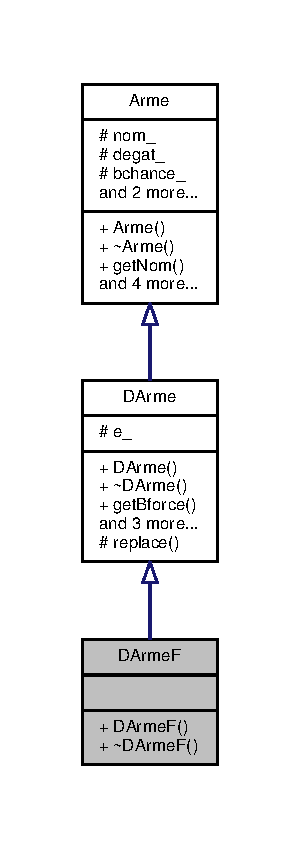
\includegraphics[width=144pt]{class_d_arme_f__inherit__graph}
\end{center}
\end{figure}


Graphe de collaboration de D\-Arme\-F\-:
\nopagebreak
\begin{figure}[H]
\begin{center}
\leavevmode
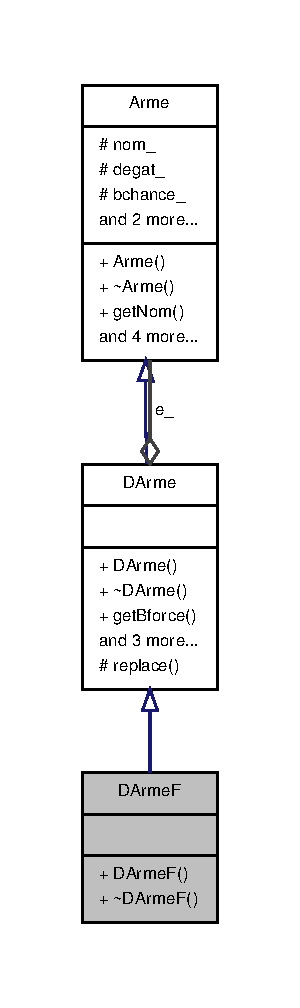
\includegraphics[width=144pt]{class_d_arme_f__coll__graph}
\end{center}
\end{figure}
\subsection*{Fonctions membres publiques}
\begin{DoxyCompactItemize}
\item 
\hypertarget{class_d_arme_f_a88e1d0ca6143fb0a00114a41ebcb7783}{{\bfseries D\-Arme\-F} (\hyperlink{class_arme}{Arme} $\ast$e)}\label{class_d_arme_f_a88e1d0ca6143fb0a00114a41ebcb7783}

\item 
int \hyperlink{class_d_arme_a76075bcbe61b20bd0e21e2d06fe33ab7}{get\-Bforce} ()
\begin{DoxyCompactList}\small\item\em Renvoie le bonus de force. \end{DoxyCompactList}\item 
int \hyperlink{class_d_arme_a91b3a3100969a568a8408ba098668398}{get\-Bvie} ()
\begin{DoxyCompactList}\small\item\em Renvoie le bonus de vie. \end{DoxyCompactList}\item 
int \hyperlink{class_d_arme_ad50d376b08d62276b7cf50d2cd59d619}{get\-Bchance} ()
\begin{DoxyCompactList}\small\item\em Renvoie le bonus de chance. \end{DoxyCompactList}\item 
int \hyperlink{class_d_arme_a7396e865674067f4f21a28e6babc0fad}{get\-Degat} ()
\begin{DoxyCompactList}\small\item\em Renvoie les dégâts. \end{DoxyCompactList}\item 
virtual std\-::string \hyperlink{class_arme_ab1b18cfa41fac19fccedf2165b9ff33c}{get\-Nom} ()
\begin{DoxyCompactList}\small\item\em Retourne le nom de l'arme. \end{DoxyCompactList}\end{DoxyCompactItemize}
\subsection*{Fonctions membres protégées}
\begin{DoxyCompactItemize}
\item 
std\-::string \hyperlink{class_d_arme_a604caa7ee656dab58d15b7cf86863e3d}{replace} (std\-::string str)
\begin{DoxyCompactList}\small\item\em Retourne le nom de l'arme modifié \end{DoxyCompactList}\end{DoxyCompactItemize}
\subsection*{Attributs protégés}
\begin{DoxyCompactItemize}
\item 
\hypertarget{class_d_arme_a03856c36a22fe5bb49f6479d0b864df2}{\hyperlink{class_arme}{Arme} $\ast$ \hyperlink{class_d_arme_a03856c36a22fe5bb49f6479d0b864df2}{e\-\_\-}}\label{class_d_arme_a03856c36a22fe5bb49f6479d0b864df2}

\begin{DoxyCompactList}\small\item\em \hyperlink{class_arme}{Arme} pour les decorations. \end{DoxyCompactList}\item 
\hypertarget{class_arme_a347394a5ab5c3230259c1b7117f3e8d6}{std\-::string \hyperlink{class_arme_a347394a5ab5c3230259c1b7117f3e8d6}{nom\-\_\-}}\label{class_arme_a347394a5ab5c3230259c1b7117f3e8d6}

\begin{DoxyCompactList}\small\item\em Nom de l'arme. \end{DoxyCompactList}\item 
\hypertarget{class_arme_a15f99a8b95c2d6f5beb9f473df79e399}{int \hyperlink{class_arme_a15f99a8b95c2d6f5beb9f473df79e399}{degat\-\_\-}}\label{class_arme_a15f99a8b95c2d6f5beb9f473df79e399}

\begin{DoxyCompactList}\small\item\em Bonus de dégat. \end{DoxyCompactList}\item 
\hypertarget{class_arme_a688792d4393f9e690aa103a8e68c541c}{int \hyperlink{class_arme_a688792d4393f9e690aa103a8e68c541c}{bchance\-\_\-}}\label{class_arme_a688792d4393f9e690aa103a8e68c541c}

\begin{DoxyCompactList}\small\item\em Bonus de chance. \end{DoxyCompactList}\item 
\hypertarget{class_arme_a4606c075b38ef49f6ed2ed06d6185173}{int \hyperlink{class_arme_a4606c075b38ef49f6ed2ed06d6185173}{bvie\-\_\-}}\label{class_arme_a4606c075b38ef49f6ed2ed06d6185173}

\begin{DoxyCompactList}\small\item\em Bonus de vie. \end{DoxyCompactList}\item 
\hypertarget{class_arme_a779e9838aa9c50d948f58b593fc5954b}{int \hyperlink{class_arme_a779e9838aa9c50d948f58b593fc5954b}{bforce\-\_\-}}\label{class_arme_a779e9838aa9c50d948f58b593fc5954b}

\begin{DoxyCompactList}\small\item\em Bonus de force. \end{DoxyCompactList}\end{DoxyCompactItemize}


\subsection{Description détaillée}
Decorator d'arme de force, hérite de \hyperlink{class_d_arme}{D\-Arme}. 

\subsection{Documentation des fonctions membres}
\hypertarget{class_d_arme_ad50d376b08d62276b7cf50d2cd59d619}{\index{D\-Arme\-F@{D\-Arme\-F}!get\-Bchance@{get\-Bchance}}
\index{get\-Bchance@{get\-Bchance}!DArmeF@{D\-Arme\-F}}
\subsubsection[{get\-Bchance}]{\setlength{\rightskip}{0pt plus 5cm}int D\-Arme\-::get\-Bchance (
\begin{DoxyParamCaption}
{}
\end{DoxyParamCaption}
)\hspace{0.3cm}{\ttfamily [virtual]}, {\ttfamily [inherited]}}}\label{class_d_arme_ad50d376b08d62276b7cf50d2cd59d619}


Renvoie le bonus de chance. 

\begin{DoxyReturn}{Renvoie}
bchance Bonus de chance 
\end{DoxyReturn}


Réimplémentée à partir de \hyperlink{class_arme_a6cb83d15008174152e424bebd0921069}{Arme}.

\hypertarget{class_d_arme_a76075bcbe61b20bd0e21e2d06fe33ab7}{\index{D\-Arme\-F@{D\-Arme\-F}!get\-Bforce@{get\-Bforce}}
\index{get\-Bforce@{get\-Bforce}!DArmeF@{D\-Arme\-F}}
\subsubsection[{get\-Bforce}]{\setlength{\rightskip}{0pt plus 5cm}int D\-Arme\-::get\-Bforce (
\begin{DoxyParamCaption}
{}
\end{DoxyParamCaption}
)\hspace{0.3cm}{\ttfamily [virtual]}, {\ttfamily [inherited]}}}\label{class_d_arme_a76075bcbe61b20bd0e21e2d06fe33ab7}


Renvoie le bonus de force. 

\begin{DoxyReturn}{Renvoie}
bforce Bonus de force 
\end{DoxyReturn}


Réimplémentée à partir de \hyperlink{class_arme_a3939e914a9ccc898de76db26bc8c24e7}{Arme}.

\hypertarget{class_d_arme_a91b3a3100969a568a8408ba098668398}{\index{D\-Arme\-F@{D\-Arme\-F}!get\-Bvie@{get\-Bvie}}
\index{get\-Bvie@{get\-Bvie}!DArmeF@{D\-Arme\-F}}
\subsubsection[{get\-Bvie}]{\setlength{\rightskip}{0pt plus 5cm}int D\-Arme\-::get\-Bvie (
\begin{DoxyParamCaption}
{}
\end{DoxyParamCaption}
)\hspace{0.3cm}{\ttfamily [virtual]}, {\ttfamily [inherited]}}}\label{class_d_arme_a91b3a3100969a568a8408ba098668398}


Renvoie le bonus de vie. 

\begin{DoxyReturn}{Renvoie}
bvie Bonus de vie 
\end{DoxyReturn}


Réimplémentée à partir de \hyperlink{class_arme_a479453fea0d6789e34ccaf193b3098ce}{Arme}.

\hypertarget{class_d_arme_a7396e865674067f4f21a28e6babc0fad}{\index{D\-Arme\-F@{D\-Arme\-F}!get\-Degat@{get\-Degat}}
\index{get\-Degat@{get\-Degat}!DArmeF@{D\-Arme\-F}}
\subsubsection[{get\-Degat}]{\setlength{\rightskip}{0pt plus 5cm}int D\-Arme\-::get\-Degat (
\begin{DoxyParamCaption}
{}
\end{DoxyParamCaption}
)\hspace{0.3cm}{\ttfamily [virtual]}, {\ttfamily [inherited]}}}\label{class_d_arme_a7396e865674067f4f21a28e6babc0fad}


Renvoie les dégâts. 

\begin{DoxyReturn}{Renvoie}
degat Dégâts 
\end{DoxyReturn}


Réimplémentée à partir de \hyperlink{class_arme_a06ced3532b0e60cc900674a94c0cf29b}{Arme}.

\hypertarget{class_arme_ab1b18cfa41fac19fccedf2165b9ff33c}{\index{D\-Arme\-F@{D\-Arme\-F}!get\-Nom@{get\-Nom}}
\index{get\-Nom@{get\-Nom}!DArmeF@{D\-Arme\-F}}
\subsubsection[{get\-Nom}]{\setlength{\rightskip}{0pt plus 5cm}std\-::string Arme\-::get\-Nom (
\begin{DoxyParamCaption}
{}
\end{DoxyParamCaption}
)\hspace{0.3cm}{\ttfamily [virtual]}, {\ttfamily [inherited]}}}\label{class_arme_ab1b18cfa41fac19fccedf2165b9ff33c}


Retourne le nom de l'arme. 

\begin{DoxyReturn}{Renvoie}
Nom 
\end{DoxyReturn}
\hypertarget{class_d_arme_a604caa7ee656dab58d15b7cf86863e3d}{\index{D\-Arme\-F@{D\-Arme\-F}!replace@{replace}}
\index{replace@{replace}!DArmeF@{D\-Arme\-F}}
\subsubsection[{replace}]{\setlength{\rightskip}{0pt plus 5cm}std\-::string D\-Arme\-::replace (
\begin{DoxyParamCaption}
\item[{std\-::string}]{str}
\end{DoxyParamCaption}
)\hspace{0.3cm}{\ttfamily [protected]}, {\ttfamily [inherited]}}}\label{class_d_arme_a604caa7ee656dab58d15b7cf86863e3d}


Retourne le nom de l'arme modifié 


\begin{DoxyParams}{Paramètres}
{\em Chaine} & de caractère à ajouter \\
\hline
\end{DoxyParams}
\begin{DoxyReturn}{Renvoie}
nom nom modifié 
\end{DoxyReturn}

\hypertarget{class_d_arme_v}{\section{Référence de la classe D\-Arme\-V}
\label{class_d_arme_v}\index{D\-Arme\-V@{D\-Arme\-V}}
}


Decorator d'arme de vie, hérite de \hyperlink{class_d_arme}{D\-Arme}.  




Graphe d'héritage de D\-Arme\-V\-:
\nopagebreak
\begin{figure}[H]
\begin{center}
\leavevmode
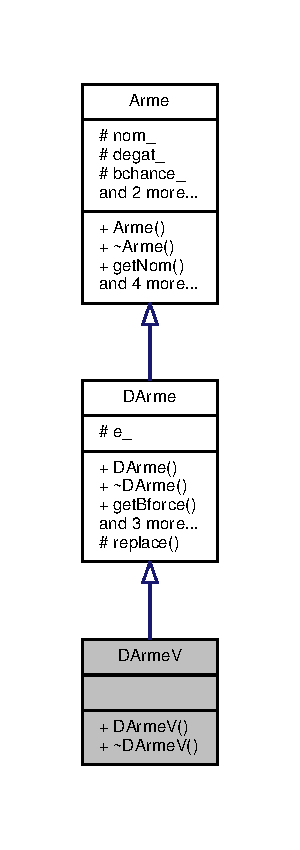
\includegraphics[width=144pt]{class_d_arme_v__inherit__graph}
\end{center}
\end{figure}


Graphe de collaboration de D\-Arme\-V\-:
\nopagebreak
\begin{figure}[H]
\begin{center}
\leavevmode
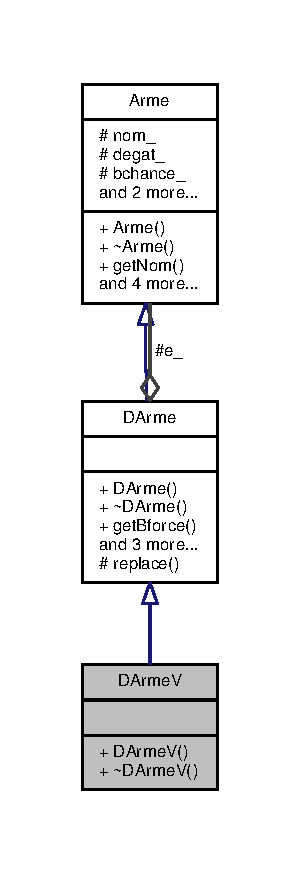
\includegraphics[width=144pt]{class_d_arme_v__coll__graph}
\end{center}
\end{figure}
\subsection*{Fonctions membres publiques}
\begin{DoxyCompactItemize}
\item 
\hypertarget{class_d_arme_v_a09195364c85ee0d457ee6d355ad179ff}{{\bfseries D\-Arme\-V} (\hyperlink{class_arme}{Arme} $\ast$e)}\label{class_d_arme_v_a09195364c85ee0d457ee6d355ad179ff}

\item 
int \hyperlink{class_d_arme_a76075bcbe61b20bd0e21e2d06fe33ab7}{get\-Bforce} ()
\begin{DoxyCompactList}\small\item\em Renvoie le bonus de force. \end{DoxyCompactList}\item 
int \hyperlink{class_d_arme_a91b3a3100969a568a8408ba098668398}{get\-Bvie} ()
\begin{DoxyCompactList}\small\item\em Renvoie le bonus de vie. \end{DoxyCompactList}\item 
int \hyperlink{class_d_arme_ad50d376b08d62276b7cf50d2cd59d619}{get\-Bchance} ()
\begin{DoxyCompactList}\small\item\em Renvoie le bonus de chance. \end{DoxyCompactList}\item 
int \hyperlink{class_d_arme_a7396e865674067f4f21a28e6babc0fad}{get\-Degat} ()
\begin{DoxyCompactList}\small\item\em Renvoie les dégâts. \end{DoxyCompactList}\item 
virtual std\-::string \hyperlink{class_arme_ab1b18cfa41fac19fccedf2165b9ff33c}{get\-Nom} ()
\begin{DoxyCompactList}\small\item\em Retourne le nom de l'arme. \end{DoxyCompactList}\end{DoxyCompactItemize}
\subsection*{Fonctions membres protégées}
\begin{DoxyCompactItemize}
\item 
std\-::string \hyperlink{class_d_arme_a604caa7ee656dab58d15b7cf86863e3d}{replace} (std\-::string str)
\begin{DoxyCompactList}\small\item\em Retourne le nom de l'arme modifié \end{DoxyCompactList}\end{DoxyCompactItemize}
\subsection*{Attributs protégés}
\begin{DoxyCompactItemize}
\item 
\hypertarget{class_d_arme_a03856c36a22fe5bb49f6479d0b864df2}{\hyperlink{class_arme}{Arme} $\ast$ \hyperlink{class_d_arme_a03856c36a22fe5bb49f6479d0b864df2}{e\-\_\-}}\label{class_d_arme_a03856c36a22fe5bb49f6479d0b864df2}

\begin{DoxyCompactList}\small\item\em \hyperlink{class_arme}{Arme} pour les decorations. \end{DoxyCompactList}\item 
\hypertarget{class_arme_a347394a5ab5c3230259c1b7117f3e8d6}{std\-::string \hyperlink{class_arme_a347394a5ab5c3230259c1b7117f3e8d6}{nom\-\_\-}}\label{class_arme_a347394a5ab5c3230259c1b7117f3e8d6}

\begin{DoxyCompactList}\small\item\em Nom de l'arme. \end{DoxyCompactList}\item 
\hypertarget{class_arme_a15f99a8b95c2d6f5beb9f473df79e399}{int \hyperlink{class_arme_a15f99a8b95c2d6f5beb9f473df79e399}{degat\-\_\-}}\label{class_arme_a15f99a8b95c2d6f5beb9f473df79e399}

\begin{DoxyCompactList}\small\item\em Bonus de dégat. \end{DoxyCompactList}\item 
\hypertarget{class_arme_a688792d4393f9e690aa103a8e68c541c}{int \hyperlink{class_arme_a688792d4393f9e690aa103a8e68c541c}{bchance\-\_\-}}\label{class_arme_a688792d4393f9e690aa103a8e68c541c}

\begin{DoxyCompactList}\small\item\em Bonus de chance. \end{DoxyCompactList}\item 
\hypertarget{class_arme_a4606c075b38ef49f6ed2ed06d6185173}{int \hyperlink{class_arme_a4606c075b38ef49f6ed2ed06d6185173}{bvie\-\_\-}}\label{class_arme_a4606c075b38ef49f6ed2ed06d6185173}

\begin{DoxyCompactList}\small\item\em Bonus de vie. \end{DoxyCompactList}\item 
\hypertarget{class_arme_a779e9838aa9c50d948f58b593fc5954b}{int \hyperlink{class_arme_a779e9838aa9c50d948f58b593fc5954b}{bforce\-\_\-}}\label{class_arme_a779e9838aa9c50d948f58b593fc5954b}

\begin{DoxyCompactList}\small\item\em Bonus de force. \end{DoxyCompactList}\end{DoxyCompactItemize}


\subsection{Description détaillée}
Decorator d'arme de vie, hérite de \hyperlink{class_d_arme}{D\-Arme}. 

\subsection{Documentation des fonctions membres}
\hypertarget{class_d_arme_ad50d376b08d62276b7cf50d2cd59d619}{\index{D\-Arme\-V@{D\-Arme\-V}!get\-Bchance@{get\-Bchance}}
\index{get\-Bchance@{get\-Bchance}!DArmeV@{D\-Arme\-V}}
\subsubsection[{get\-Bchance}]{\setlength{\rightskip}{0pt plus 5cm}int D\-Arme\-::get\-Bchance (
\begin{DoxyParamCaption}
{}
\end{DoxyParamCaption}
)\hspace{0.3cm}{\ttfamily [virtual]}, {\ttfamily [inherited]}}}\label{class_d_arme_ad50d376b08d62276b7cf50d2cd59d619}


Renvoie le bonus de chance. 

\begin{DoxyReturn}{Renvoie}
bchance Bonus de chance 
\end{DoxyReturn}


Réimplémentée à partir de \hyperlink{class_arme_a6cb83d15008174152e424bebd0921069}{Arme}.

\hypertarget{class_d_arme_a76075bcbe61b20bd0e21e2d06fe33ab7}{\index{D\-Arme\-V@{D\-Arme\-V}!get\-Bforce@{get\-Bforce}}
\index{get\-Bforce@{get\-Bforce}!DArmeV@{D\-Arme\-V}}
\subsubsection[{get\-Bforce}]{\setlength{\rightskip}{0pt plus 5cm}int D\-Arme\-::get\-Bforce (
\begin{DoxyParamCaption}
{}
\end{DoxyParamCaption}
)\hspace{0.3cm}{\ttfamily [virtual]}, {\ttfamily [inherited]}}}\label{class_d_arme_a76075bcbe61b20bd0e21e2d06fe33ab7}


Renvoie le bonus de force. 

\begin{DoxyReturn}{Renvoie}
bforce Bonus de force 
\end{DoxyReturn}


Réimplémentée à partir de \hyperlink{class_arme_a3939e914a9ccc898de76db26bc8c24e7}{Arme}.

\hypertarget{class_d_arme_a91b3a3100969a568a8408ba098668398}{\index{D\-Arme\-V@{D\-Arme\-V}!get\-Bvie@{get\-Bvie}}
\index{get\-Bvie@{get\-Bvie}!DArmeV@{D\-Arme\-V}}
\subsubsection[{get\-Bvie}]{\setlength{\rightskip}{0pt plus 5cm}int D\-Arme\-::get\-Bvie (
\begin{DoxyParamCaption}
{}
\end{DoxyParamCaption}
)\hspace{0.3cm}{\ttfamily [virtual]}, {\ttfamily [inherited]}}}\label{class_d_arme_a91b3a3100969a568a8408ba098668398}


Renvoie le bonus de vie. 

\begin{DoxyReturn}{Renvoie}
bvie Bonus de vie 
\end{DoxyReturn}


Réimplémentée à partir de \hyperlink{class_arme_a479453fea0d6789e34ccaf193b3098ce}{Arme}.

\hypertarget{class_d_arme_a7396e865674067f4f21a28e6babc0fad}{\index{D\-Arme\-V@{D\-Arme\-V}!get\-Degat@{get\-Degat}}
\index{get\-Degat@{get\-Degat}!DArmeV@{D\-Arme\-V}}
\subsubsection[{get\-Degat}]{\setlength{\rightskip}{0pt plus 5cm}int D\-Arme\-::get\-Degat (
\begin{DoxyParamCaption}
{}
\end{DoxyParamCaption}
)\hspace{0.3cm}{\ttfamily [virtual]}, {\ttfamily [inherited]}}}\label{class_d_arme_a7396e865674067f4f21a28e6babc0fad}


Renvoie les dégâts. 

\begin{DoxyReturn}{Renvoie}
degat Dégâts 
\end{DoxyReturn}


Réimplémentée à partir de \hyperlink{class_arme_a06ced3532b0e60cc900674a94c0cf29b}{Arme}.

\hypertarget{class_arme_ab1b18cfa41fac19fccedf2165b9ff33c}{\index{D\-Arme\-V@{D\-Arme\-V}!get\-Nom@{get\-Nom}}
\index{get\-Nom@{get\-Nom}!DArmeV@{D\-Arme\-V}}
\subsubsection[{get\-Nom}]{\setlength{\rightskip}{0pt plus 5cm}std\-::string Arme\-::get\-Nom (
\begin{DoxyParamCaption}
{}
\end{DoxyParamCaption}
)\hspace{0.3cm}{\ttfamily [virtual]}, {\ttfamily [inherited]}}}\label{class_arme_ab1b18cfa41fac19fccedf2165b9ff33c}


Retourne le nom de l'arme. 

\begin{DoxyReturn}{Renvoie}
Nom 
\end{DoxyReturn}
\hypertarget{class_d_arme_a604caa7ee656dab58d15b7cf86863e3d}{\index{D\-Arme\-V@{D\-Arme\-V}!replace@{replace}}
\index{replace@{replace}!DArmeV@{D\-Arme\-V}}
\subsubsection[{replace}]{\setlength{\rightskip}{0pt plus 5cm}std\-::string D\-Arme\-::replace (
\begin{DoxyParamCaption}
\item[{std\-::string}]{str}
\end{DoxyParamCaption}
)\hspace{0.3cm}{\ttfamily [protected]}, {\ttfamily [inherited]}}}\label{class_d_arme_a604caa7ee656dab58d15b7cf86863e3d}


Retourne le nom de l'arme modifié 


\begin{DoxyParams}{Paramètres}
{\em Chaine} & de caractère à ajouter \\
\hline
\end{DoxyParams}
\begin{DoxyReturn}{Renvoie}
nom nom modifié 
\end{DoxyReturn}

\section{Référence de la classe D\-Equip}
\label{class_d_equip}\index{D\-Equip@{D\-Equip}}


Decorator d'équipement , hérite de \doxyref{Equipement}{p.}{class_equipement}.  




Graphe d'héritage de D\-Equip\-:\nopagebreak
\begin{figure}[H]
\begin{center}
\leavevmode
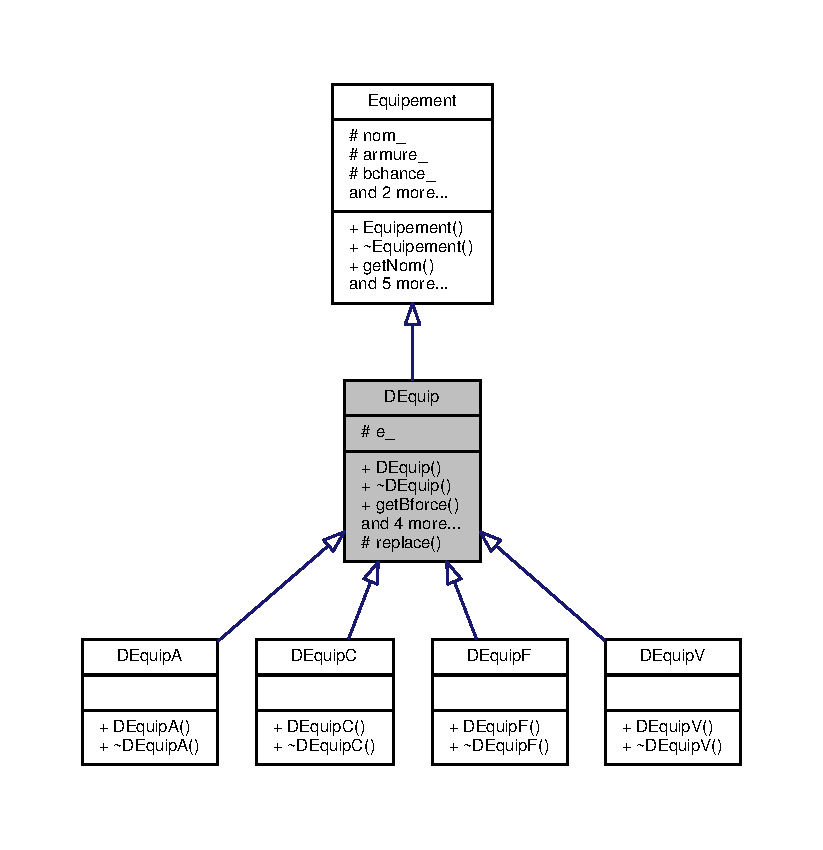
\includegraphics[width=350pt]{class_d_equip__inherit__graph}
\end{center}
\end{figure}


Graphe de collaboration de D\-Equip\-:\nopagebreak
\begin{figure}[H]
\begin{center}
\leavevmode
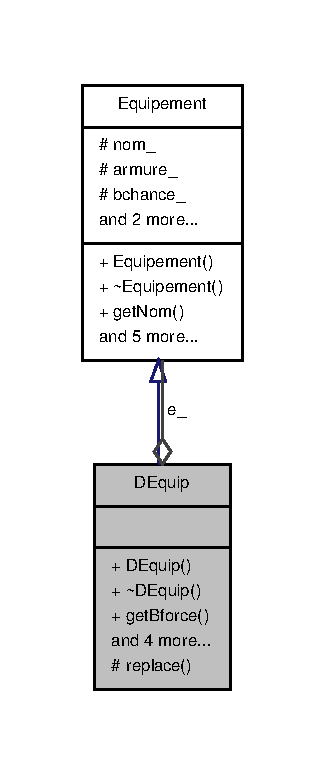
\includegraphics[width=156pt]{class_d_equip__coll__graph}
\end{center}
\end{figure}
\subsection*{Fonctions membres publiques}
\begin{DoxyCompactItemize}
\item 
{\bf D\-Equip} ({\bf Equipement} $\ast$e)
\begin{DoxyCompactList}\small\item\em Constructeur du décorator d'\doxyref{Equipement}{p.}{class_equipement}. \end{DoxyCompactList}\item 
{\bf $\sim$\-D\-Equip} ()
\item 
int {\bf get\-Bforce} ()
\begin{DoxyCompactList}\small\item\em Renvoie le bonus de force. \end{DoxyCompactList}\item 
int {\bf get\-Bvie} ()
\begin{DoxyCompactList}\small\item\em Renvoie le bonus de vie. \end{DoxyCompactList}\item 
int {\bf get\-Bchance} ()
\begin{DoxyCompactList}\small\item\em Renvoie le bonus de chance. \end{DoxyCompactList}\item 
int {\bf get\-Armure} ()
\begin{DoxyCompactList}\small\item\em Renvoie le bonus d'armure. \end{DoxyCompactList}\item 
int {\bf type} ()
\begin{DoxyCompactList}\small\item\em Renvoie le type de l'\doxyref{Equipement}{p.}{class_equipement}. \end{DoxyCompactList}\item 
virtual std\-::string {\bf get\-Nom} ()
\begin{DoxyCompactList}\small\item\em Retourne le nom de l'equipement. \end{DoxyCompactList}\end{DoxyCompactItemize}
\subsection*{Fonctions membres protégées}
\begin{DoxyCompactItemize}
\item 
std\-::string {\bf replace} (std\-::string str)
\begin{DoxyCompactList}\small\item\em Retourne le nom de l'équipement modifié \end{DoxyCompactList}\end{DoxyCompactItemize}
\subsection*{Attributs protégés}
\begin{DoxyCompactItemize}
\item 
{\bf Equipement} $\ast$ {\bf e\-\_\-}
\begin{DoxyCompactList}\small\item\em \doxyref{Equipement}{p.}{class_equipement} e pour la décoration. \end{DoxyCompactList}\item 
std\-::string {\bf nom\-\_\-}
\item 
int {\bf armure\-\_\-}
\item 
int {\bf bchance\-\_\-}
\item 
int {\bf bvie\-\_\-}
\item 
int {\bf bforce\-\_\-}
\end{DoxyCompactItemize}


\subsection{Description détaillée}
Decorator d'équipement , hérite de \doxyref{Equipement}{p.}{class_equipement}. 

\subsection{Documentation des constructeurs et destructeur}
\index{D\-Equip@{D\-Equip}!D\-Equip@{D\-Equip}}
\index{D\-Equip@{D\-Equip}!DEquip@{D\-Equip}}
\subsubsection[{D\-Equip}]{\setlength{\rightskip}{0pt plus 5cm}D\-Equip\-::\-D\-Equip (
\begin{DoxyParamCaption}
\item[{{\bf Equipement} $\ast$}]{e}
\end{DoxyParamCaption}
)}\label{class_d_equip_a1e7c01de5a65a38e5699b6d4679e8422}


Constructeur du décorator d'\doxyref{Equipement}{p.}{class_equipement}. 

\index{D\-Equip@{D\-Equip}!$\sim$\-D\-Equip@{$\sim$\-D\-Equip}}
\index{$\sim$\-D\-Equip@{$\sim$\-D\-Equip}!DEquip@{D\-Equip}}
\subsubsection[{$\sim$\-D\-Equip}]{\setlength{\rightskip}{0pt plus 5cm}D\-Equip\-::$\sim$\-D\-Equip (
\begin{DoxyParamCaption}
{}
\end{DoxyParamCaption}
)}\label{class_d_equip_a52a73a6b6cbd9bca7523eedafd90f3ef}


\subsection{Documentation des fonctions membres}
\index{D\-Equip@{D\-Equip}!get\-Armure@{get\-Armure}}
\index{get\-Armure@{get\-Armure}!DEquip@{D\-Equip}}
\subsubsection[{get\-Armure}]{\setlength{\rightskip}{0pt plus 5cm}int D\-Equip\-::get\-Armure (
\begin{DoxyParamCaption}
{}
\end{DoxyParamCaption}
)\hspace{0.3cm}{\ttfamily [virtual]}}\label{class_d_equip_a7b2c8227ae884c23ccc8f3a2e5702186}


Renvoie le bonus d'armure. 

\begin{DoxyReturn}{Renvoie}
armure Bonus d'armure 
\end{DoxyReturn}


Réimplémentée à partir de {\bf Equipement} \doxyref{}{p.}{class_equipement_a8577d49fd00b8effa39388feccb29901}.

\index{D\-Equip@{D\-Equip}!get\-Bchance@{get\-Bchance}}
\index{get\-Bchance@{get\-Bchance}!DEquip@{D\-Equip}}
\subsubsection[{get\-Bchance}]{\setlength{\rightskip}{0pt plus 5cm}int D\-Equip\-::get\-Bchance (
\begin{DoxyParamCaption}
{}
\end{DoxyParamCaption}
)\hspace{0.3cm}{\ttfamily [virtual]}}\label{class_d_equip_a39407c92f0de87306a33f57fd22ce997}


Renvoie le bonus de chance. 

\begin{DoxyReturn}{Renvoie}
bchance Bonus de chance 
\end{DoxyReturn}


Réimplémentée à partir de {\bf Equipement} \doxyref{}{p.}{class_equipement_a73485135eacdf30d5f49c9e34e5f4d0e}.

\index{D\-Equip@{D\-Equip}!get\-Bforce@{get\-Bforce}}
\index{get\-Bforce@{get\-Bforce}!DEquip@{D\-Equip}}
\subsubsection[{get\-Bforce}]{\setlength{\rightskip}{0pt plus 5cm}int D\-Equip\-::get\-Bforce (
\begin{DoxyParamCaption}
{}
\end{DoxyParamCaption}
)\hspace{0.3cm}{\ttfamily [virtual]}}\label{class_d_equip_adb6645ce01c12a4cb3fe0b522ea6b25e}


Renvoie le bonus de force. 

\begin{DoxyReturn}{Renvoie}
bforce Bonus de force 
\end{DoxyReturn}


Réimplémentée à partir de {\bf Equipement} \doxyref{}{p.}{class_equipement_aabcf10fd762945fa4a37a9cf8321f463}.

\index{D\-Equip@{D\-Equip}!get\-Bvie@{get\-Bvie}}
\index{get\-Bvie@{get\-Bvie}!DEquip@{D\-Equip}}
\subsubsection[{get\-Bvie}]{\setlength{\rightskip}{0pt plus 5cm}int D\-Equip\-::get\-Bvie (
\begin{DoxyParamCaption}
{}
\end{DoxyParamCaption}
)\hspace{0.3cm}{\ttfamily [virtual]}}\label{class_d_equip_a085ea4ac21c238d8c147ff4e6d74794f}


Renvoie le bonus de vie. 

\begin{DoxyReturn}{Renvoie}
bvie Bonus de vie 
\end{DoxyReturn}


Réimplémentée à partir de {\bf Equipement} \doxyref{}{p.}{class_equipement_ad9fd7528c4f181970b7a0877f4145f89}.

\index{D\-Equip@{D\-Equip}!get\-Nom@{get\-Nom}}
\index{get\-Nom@{get\-Nom}!DEquip@{D\-Equip}}
\subsubsection[{get\-Nom}]{\setlength{\rightskip}{0pt plus 5cm}std\-::string Equipement\-::get\-Nom (
\begin{DoxyParamCaption}
{}
\end{DoxyParamCaption}
)\hspace{0.3cm}{\ttfamily [virtual]}, {\ttfamily [inherited]}}\label{class_equipement_a0b0426a70bfce6e7c3efac605b75cd8e}


Retourne le nom de l'equipement. 

\begin{DoxyReturn}{Renvoie}
Nom 
\end{DoxyReturn}
\index{D\-Equip@{D\-Equip}!replace@{replace}}
\index{replace@{replace}!DEquip@{D\-Equip}}
\subsubsection[{replace}]{\setlength{\rightskip}{0pt plus 5cm}std\-::string D\-Equip\-::replace (
\begin{DoxyParamCaption}
\item[{std\-::string}]{str}
\end{DoxyParamCaption}
)\hspace{0.3cm}{\ttfamily [protected]}}\label{class_d_equip_af8a7e83f36094af1f34f5c81df6e3900}


Retourne le nom de l'équipement modifié 


\begin{DoxyParams}{Paramètres}
{\em Chaine} & de caractère à ajouter \\
\hline
\end{DoxyParams}
\begin{DoxyReturn}{Renvoie}
nom nom modifié 
\end{DoxyReturn}
\index{D\-Equip@{D\-Equip}!type@{type}}
\index{type@{type}!DEquip@{D\-Equip}}
\subsubsection[{type}]{\setlength{\rightskip}{0pt plus 5cm}int D\-Equip\-::type (
\begin{DoxyParamCaption}
{}
\end{DoxyParamCaption}
)\hspace{0.3cm}{\ttfamily [virtual]}}\label{class_d_equip_a7c31f807517e5940e899780ac6d7a5c3}


Renvoie le type de l'\doxyref{Equipement}{p.}{class_equipement}. 

\begin{DoxyReturn}{Renvoie}
entier type de l'\doxyref{Equipement}{p.}{class_equipement} 
\end{DoxyReturn}


Implémente {\bf Equipement} \doxyref{}{p.}{class_equipement_a05b2c9d4cf22b6aefb6603fa4e322aa2}.



\subsection{Documentation des données membres}
\index{D\-Equip@{D\-Equip}!armure\-\_\-@{armure\-\_\-}}
\index{armure\-\_\-@{armure\-\_\-}!DEquip@{D\-Equip}}
\subsubsection[{armure\-\_\-}]{\setlength{\rightskip}{0pt plus 5cm}int Equipement\-::armure\-\_\-\hspace{0.3cm}{\ttfamily [protected]}, {\ttfamily [inherited]}}\label{class_equipement_a69339ce4f1f5fe7e6fcdeda5b74c14a4}
\index{D\-Equip@{D\-Equip}!bchance\-\_\-@{bchance\-\_\-}}
\index{bchance\-\_\-@{bchance\-\_\-}!DEquip@{D\-Equip}}
\subsubsection[{bchance\-\_\-}]{\setlength{\rightskip}{0pt plus 5cm}int Equipement\-::bchance\-\_\-\hspace{0.3cm}{\ttfamily [protected]}, {\ttfamily [inherited]}}\label{class_equipement_aa70effa6a8144fe1f4fe874af7139793}
\index{D\-Equip@{D\-Equip}!bforce\-\_\-@{bforce\-\_\-}}
\index{bforce\-\_\-@{bforce\-\_\-}!DEquip@{D\-Equip}}
\subsubsection[{bforce\-\_\-}]{\setlength{\rightskip}{0pt plus 5cm}int Equipement\-::bforce\-\_\-\hspace{0.3cm}{\ttfamily [protected]}, {\ttfamily [inherited]}}\label{class_equipement_af87cf3f291386d5401be6994dd8fb8be}
\index{D\-Equip@{D\-Equip}!bvie\-\_\-@{bvie\-\_\-}}
\index{bvie\-\_\-@{bvie\-\_\-}!DEquip@{D\-Equip}}
\subsubsection[{bvie\-\_\-}]{\setlength{\rightskip}{0pt plus 5cm}int Equipement\-::bvie\-\_\-\hspace{0.3cm}{\ttfamily [protected]}, {\ttfamily [inherited]}}\label{class_equipement_a73ac5bff40e3f6bf1d8e6f0e524e750f}
\index{D\-Equip@{D\-Equip}!e\-\_\-@{e\-\_\-}}
\index{e\-\_\-@{e\-\_\-}!DEquip@{D\-Equip}}
\subsubsection[{e\-\_\-}]{\setlength{\rightskip}{0pt plus 5cm}{\bf Equipement}$\ast$ D\-Equip\-::e\-\_\-\hspace{0.3cm}{\ttfamily [protected]}}\label{class_d_equip_a0243fb57df463a3d0a7c57e6e7980210}


\doxyref{Equipement}{p.}{class_equipement} e pour la décoration. 

\index{D\-Equip@{D\-Equip}!nom\-\_\-@{nom\-\_\-}}
\index{nom\-\_\-@{nom\-\_\-}!DEquip@{D\-Equip}}
\subsubsection[{nom\-\_\-}]{\setlength{\rightskip}{0pt plus 5cm}std\-::string Equipement\-::nom\-\_\-\hspace{0.3cm}{\ttfamily [protected]}, {\ttfamily [inherited]}}\label{class_equipement_a930290aac01ecd40c7a646ab8f66d742}


La documentation de cette classe a été générée à partir des fichiers suivants \-:\begin{DoxyCompactItemize}
\item 
src/{\bf D\-Equip.\-hpp}\item 
src/{\bf D\-Equip.\-cpp}\end{DoxyCompactItemize}

\section{Référence de la classe D\-Equip\-A}
\label{class_d_equip_a}\index{D\-Equip\-A@{D\-Equip\-A}}


Decorator d'équipement d'armure , hérite de \doxyref{D\-Equip}{p.}{class_d_equip}.  




Graphe d'héritage de D\-Equip\-A\-:\nopagebreak
\begin{figure}[H]
\begin{center}
\leavevmode
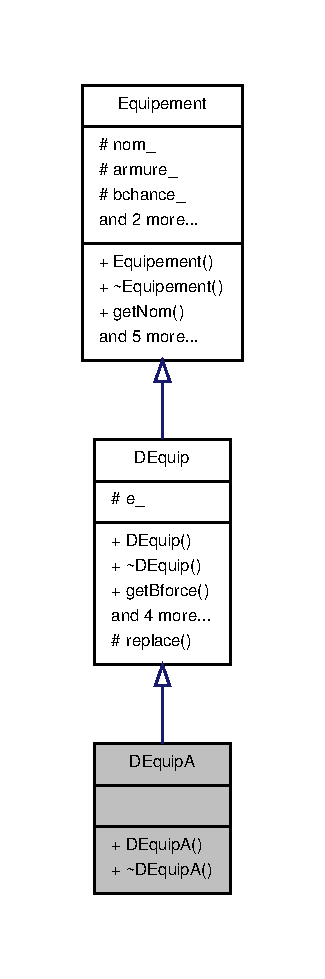
\includegraphics[width=156pt]{class_d_equip_a__inherit__graph}
\end{center}
\end{figure}


Graphe de collaboration de D\-Equip\-A\-:\nopagebreak
\begin{figure}[H]
\begin{center}
\leavevmode
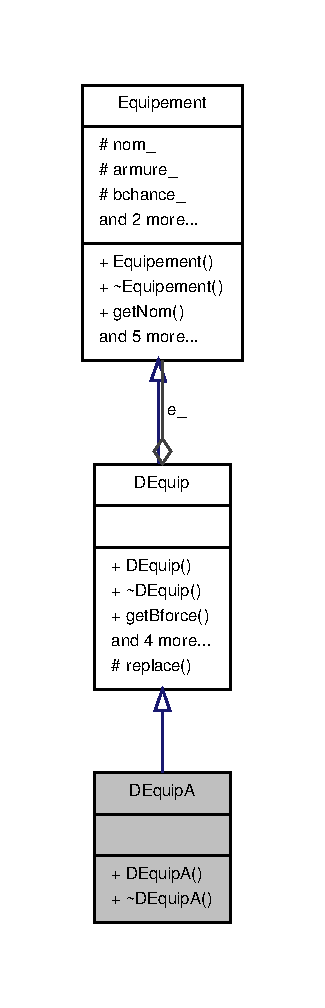
\includegraphics[width=156pt]{class_d_equip_a__coll__graph}
\end{center}
\end{figure}
\subsection*{Fonctions membres publiques}
\begin{DoxyCompactItemize}
\item 
{\bf D\-Equip\-A} ({\bf Equipement} $\ast$e)
\item 
{\bf $\sim$\-D\-Equip\-A} ()
\item 
int {\bf get\-Bforce} ()
\begin{DoxyCompactList}\small\item\em Renvoie le bonus de force. \end{DoxyCompactList}\item 
int {\bf get\-Bvie} ()
\begin{DoxyCompactList}\small\item\em Renvoie le bonus de vie. \end{DoxyCompactList}\item 
int {\bf get\-Bchance} ()
\begin{DoxyCompactList}\small\item\em Renvoie le bonus de chance. \end{DoxyCompactList}\item 
int {\bf get\-Armure} ()
\begin{DoxyCompactList}\small\item\em Renvoie le bonus d'armure. \end{DoxyCompactList}\item 
int {\bf type} ()
\begin{DoxyCompactList}\small\item\em Renvoie le type de l'\doxyref{Equipement}{p.}{class_equipement}. \end{DoxyCompactList}\item 
virtual std\-::string {\bf get\-Nom} ()
\begin{DoxyCompactList}\small\item\em Retourne le nom de l'equipement. \end{DoxyCompactList}\end{DoxyCompactItemize}
\subsection*{Fonctions membres protégées}
\begin{DoxyCompactItemize}
\item 
std\-::string {\bf replace} (std\-::string str)
\begin{DoxyCompactList}\small\item\em Retourne le nom de l'équipement modifié \end{DoxyCompactList}\end{DoxyCompactItemize}
\subsection*{Attributs protégés}
\begin{DoxyCompactItemize}
\item 
{\bf Equipement} $\ast$ {\bf e\-\_\-}
\begin{DoxyCompactList}\small\item\em \doxyref{Equipement}{p.}{class_equipement} e pour la décoration. \end{DoxyCompactList}\item 
std\-::string {\bf nom\-\_\-}
\item 
int {\bf armure\-\_\-}
\item 
int {\bf bchance\-\_\-}
\item 
int {\bf bvie\-\_\-}
\item 
int {\bf bforce\-\_\-}
\end{DoxyCompactItemize}


\subsection{Description détaillée}
Decorator d'équipement d'armure , hérite de \doxyref{D\-Equip}{p.}{class_d_equip}. 

\subsection{Documentation des constructeurs et destructeur}
\index{D\-Equip\-A@{D\-Equip\-A}!D\-Equip\-A@{D\-Equip\-A}}
\index{D\-Equip\-A@{D\-Equip\-A}!DEquipA@{D\-Equip\-A}}
\subsubsection[{D\-Equip\-A}]{\setlength{\rightskip}{0pt plus 5cm}D\-Equip\-A\-::\-D\-Equip\-A (
\begin{DoxyParamCaption}
\item[{{\bf Equipement} $\ast$}]{e}
\end{DoxyParamCaption}
)}\label{class_d_equip_a_acbbaea66a8f555ba74e83e287df9fd4c}
\index{D\-Equip\-A@{D\-Equip\-A}!$\sim$\-D\-Equip\-A@{$\sim$\-D\-Equip\-A}}
\index{$\sim$\-D\-Equip\-A@{$\sim$\-D\-Equip\-A}!DEquipA@{D\-Equip\-A}}
\subsubsection[{$\sim$\-D\-Equip\-A}]{\setlength{\rightskip}{0pt plus 5cm}D\-Equip\-A\-::$\sim$\-D\-Equip\-A (
\begin{DoxyParamCaption}
{}
\end{DoxyParamCaption}
)}\label{class_d_equip_a_af71b86145c078bd192f1267c8dc95991}


\subsection{Documentation des fonctions membres}
\index{D\-Equip\-A@{D\-Equip\-A}!get\-Armure@{get\-Armure}}
\index{get\-Armure@{get\-Armure}!DEquipA@{D\-Equip\-A}}
\subsubsection[{get\-Armure}]{\setlength{\rightskip}{0pt plus 5cm}int D\-Equip\-::get\-Armure (
\begin{DoxyParamCaption}
{}
\end{DoxyParamCaption}
)\hspace{0.3cm}{\ttfamily [virtual]}, {\ttfamily [inherited]}}\label{class_d_equip_a7b2c8227ae884c23ccc8f3a2e5702186}


Renvoie le bonus d'armure. 

\begin{DoxyReturn}{Renvoie}
armure Bonus d'armure 
\end{DoxyReturn}


Réimplémentée à partir de {\bf Equipement} \doxyref{}{p.}{class_equipement_a8577d49fd00b8effa39388feccb29901}.

\index{D\-Equip\-A@{D\-Equip\-A}!get\-Bchance@{get\-Bchance}}
\index{get\-Bchance@{get\-Bchance}!DEquipA@{D\-Equip\-A}}
\subsubsection[{get\-Bchance}]{\setlength{\rightskip}{0pt plus 5cm}int D\-Equip\-::get\-Bchance (
\begin{DoxyParamCaption}
{}
\end{DoxyParamCaption}
)\hspace{0.3cm}{\ttfamily [virtual]}, {\ttfamily [inherited]}}\label{class_d_equip_a39407c92f0de87306a33f57fd22ce997}


Renvoie le bonus de chance. 

\begin{DoxyReturn}{Renvoie}
bchance Bonus de chance 
\end{DoxyReturn}


Réimplémentée à partir de {\bf Equipement} \doxyref{}{p.}{class_equipement_a73485135eacdf30d5f49c9e34e5f4d0e}.

\index{D\-Equip\-A@{D\-Equip\-A}!get\-Bforce@{get\-Bforce}}
\index{get\-Bforce@{get\-Bforce}!DEquipA@{D\-Equip\-A}}
\subsubsection[{get\-Bforce}]{\setlength{\rightskip}{0pt plus 5cm}int D\-Equip\-::get\-Bforce (
\begin{DoxyParamCaption}
{}
\end{DoxyParamCaption}
)\hspace{0.3cm}{\ttfamily [virtual]}, {\ttfamily [inherited]}}\label{class_d_equip_adb6645ce01c12a4cb3fe0b522ea6b25e}


Renvoie le bonus de force. 

\begin{DoxyReturn}{Renvoie}
bforce Bonus de force 
\end{DoxyReturn}


Réimplémentée à partir de {\bf Equipement} \doxyref{}{p.}{class_equipement_aabcf10fd762945fa4a37a9cf8321f463}.

\index{D\-Equip\-A@{D\-Equip\-A}!get\-Bvie@{get\-Bvie}}
\index{get\-Bvie@{get\-Bvie}!DEquipA@{D\-Equip\-A}}
\subsubsection[{get\-Bvie}]{\setlength{\rightskip}{0pt plus 5cm}int D\-Equip\-::get\-Bvie (
\begin{DoxyParamCaption}
{}
\end{DoxyParamCaption}
)\hspace{0.3cm}{\ttfamily [virtual]}, {\ttfamily [inherited]}}\label{class_d_equip_a085ea4ac21c238d8c147ff4e6d74794f}


Renvoie le bonus de vie. 

\begin{DoxyReturn}{Renvoie}
bvie Bonus de vie 
\end{DoxyReturn}


Réimplémentée à partir de {\bf Equipement} \doxyref{}{p.}{class_equipement_ad9fd7528c4f181970b7a0877f4145f89}.

\index{D\-Equip\-A@{D\-Equip\-A}!get\-Nom@{get\-Nom}}
\index{get\-Nom@{get\-Nom}!DEquipA@{D\-Equip\-A}}
\subsubsection[{get\-Nom}]{\setlength{\rightskip}{0pt plus 5cm}std\-::string Equipement\-::get\-Nom (
\begin{DoxyParamCaption}
{}
\end{DoxyParamCaption}
)\hspace{0.3cm}{\ttfamily [virtual]}, {\ttfamily [inherited]}}\label{class_equipement_a0b0426a70bfce6e7c3efac605b75cd8e}


Retourne le nom de l'equipement. 

\begin{DoxyReturn}{Renvoie}
Nom 
\end{DoxyReturn}
\index{D\-Equip\-A@{D\-Equip\-A}!replace@{replace}}
\index{replace@{replace}!DEquipA@{D\-Equip\-A}}
\subsubsection[{replace}]{\setlength{\rightskip}{0pt plus 5cm}std\-::string D\-Equip\-::replace (
\begin{DoxyParamCaption}
\item[{std\-::string}]{str}
\end{DoxyParamCaption}
)\hspace{0.3cm}{\ttfamily [protected]}, {\ttfamily [inherited]}}\label{class_d_equip_af8a7e83f36094af1f34f5c81df6e3900}


Retourne le nom de l'équipement modifié 


\begin{DoxyParams}{Paramètres}
{\em Chaine} & de caractère à ajouter \\
\hline
\end{DoxyParams}
\begin{DoxyReturn}{Renvoie}
nom nom modifié 
\end{DoxyReturn}
\index{D\-Equip\-A@{D\-Equip\-A}!type@{type}}
\index{type@{type}!DEquipA@{D\-Equip\-A}}
\subsubsection[{type}]{\setlength{\rightskip}{0pt plus 5cm}int D\-Equip\-::type (
\begin{DoxyParamCaption}
{}
\end{DoxyParamCaption}
)\hspace{0.3cm}{\ttfamily [virtual]}, {\ttfamily [inherited]}}\label{class_d_equip_a7c31f807517e5940e899780ac6d7a5c3}


Renvoie le type de l'\doxyref{Equipement}{p.}{class_equipement}. 

\begin{DoxyReturn}{Renvoie}
entier type de l'\doxyref{Equipement}{p.}{class_equipement} 
\end{DoxyReturn}


Implémente {\bf Equipement} \doxyref{}{p.}{class_equipement_a05b2c9d4cf22b6aefb6603fa4e322aa2}.



\subsection{Documentation des données membres}
\index{D\-Equip\-A@{D\-Equip\-A}!armure\-\_\-@{armure\-\_\-}}
\index{armure\-\_\-@{armure\-\_\-}!DEquipA@{D\-Equip\-A}}
\subsubsection[{armure\-\_\-}]{\setlength{\rightskip}{0pt plus 5cm}int Equipement\-::armure\-\_\-\hspace{0.3cm}{\ttfamily [protected]}, {\ttfamily [inherited]}}\label{class_equipement_a69339ce4f1f5fe7e6fcdeda5b74c14a4}
\index{D\-Equip\-A@{D\-Equip\-A}!bchance\-\_\-@{bchance\-\_\-}}
\index{bchance\-\_\-@{bchance\-\_\-}!DEquipA@{D\-Equip\-A}}
\subsubsection[{bchance\-\_\-}]{\setlength{\rightskip}{0pt plus 5cm}int Equipement\-::bchance\-\_\-\hspace{0.3cm}{\ttfamily [protected]}, {\ttfamily [inherited]}}\label{class_equipement_aa70effa6a8144fe1f4fe874af7139793}
\index{D\-Equip\-A@{D\-Equip\-A}!bforce\-\_\-@{bforce\-\_\-}}
\index{bforce\-\_\-@{bforce\-\_\-}!DEquipA@{D\-Equip\-A}}
\subsubsection[{bforce\-\_\-}]{\setlength{\rightskip}{0pt plus 5cm}int Equipement\-::bforce\-\_\-\hspace{0.3cm}{\ttfamily [protected]}, {\ttfamily [inherited]}}\label{class_equipement_af87cf3f291386d5401be6994dd8fb8be}
\index{D\-Equip\-A@{D\-Equip\-A}!bvie\-\_\-@{bvie\-\_\-}}
\index{bvie\-\_\-@{bvie\-\_\-}!DEquipA@{D\-Equip\-A}}
\subsubsection[{bvie\-\_\-}]{\setlength{\rightskip}{0pt plus 5cm}int Equipement\-::bvie\-\_\-\hspace{0.3cm}{\ttfamily [protected]}, {\ttfamily [inherited]}}\label{class_equipement_a73ac5bff40e3f6bf1d8e6f0e524e750f}
\index{D\-Equip\-A@{D\-Equip\-A}!e\-\_\-@{e\-\_\-}}
\index{e\-\_\-@{e\-\_\-}!DEquipA@{D\-Equip\-A}}
\subsubsection[{e\-\_\-}]{\setlength{\rightskip}{0pt plus 5cm}{\bf Equipement}$\ast$ D\-Equip\-::e\-\_\-\hspace{0.3cm}{\ttfamily [protected]}, {\ttfamily [inherited]}}\label{class_d_equip_a0243fb57df463a3d0a7c57e6e7980210}


\doxyref{Equipement}{p.}{class_equipement} e pour la décoration. 

\index{D\-Equip\-A@{D\-Equip\-A}!nom\-\_\-@{nom\-\_\-}}
\index{nom\-\_\-@{nom\-\_\-}!DEquipA@{D\-Equip\-A}}
\subsubsection[{nom\-\_\-}]{\setlength{\rightskip}{0pt plus 5cm}std\-::string Equipement\-::nom\-\_\-\hspace{0.3cm}{\ttfamily [protected]}, {\ttfamily [inherited]}}\label{class_equipement_a930290aac01ecd40c7a646ab8f66d742}


La documentation de cette classe a été générée à partir des fichiers suivants \-:\begin{DoxyCompactItemize}
\item 
src/{\bf D\-Equip\-A.\-hpp}\item 
src/{\bf D\-Equip\-A.\-cpp}\end{DoxyCompactItemize}

\hypertarget{class_d_equip_c}{\section{Référence de la classe D\-Equip\-C}
\label{class_d_equip_c}\index{D\-Equip\-C@{D\-Equip\-C}}
}


Decorator d'équipement de chance , hérite de \hyperlink{class_d_equip}{D\-Equip}.  




Graphe d'héritage de D\-Equip\-C\-:
\nopagebreak
\begin{figure}[H]
\begin{center}
\leavevmode
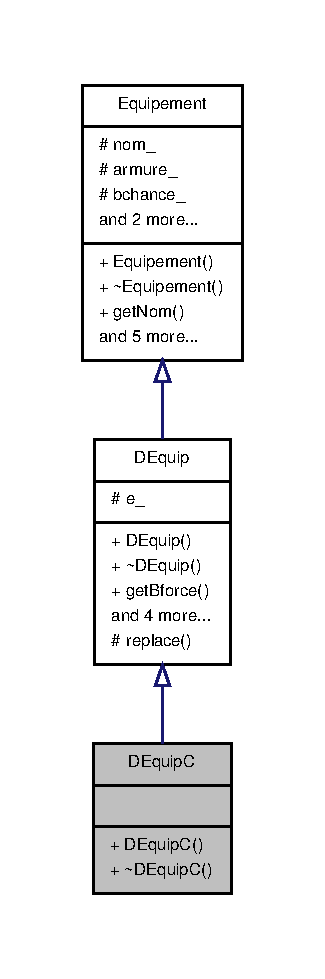
\includegraphics[width=156pt]{class_d_equip_c__inherit__graph}
\end{center}
\end{figure}


Graphe de collaboration de D\-Equip\-C\-:
\nopagebreak
\begin{figure}[H]
\begin{center}
\leavevmode
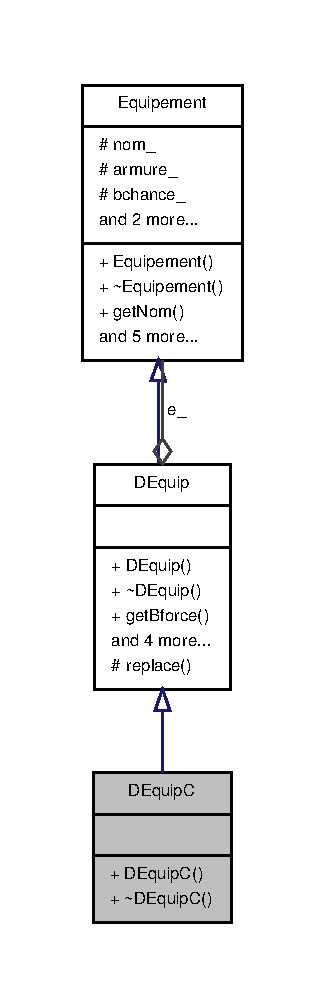
\includegraphics[width=156pt]{class_d_equip_c__coll__graph}
\end{center}
\end{figure}
\subsection*{Fonctions membres publiques}
\begin{DoxyCompactItemize}
\item 
\hypertarget{class_d_equip_c_a84b4ff1ea2ee4a70f48bdbfe5b8507ed}{{\bfseries D\-Equip\-C} (\hyperlink{class_equipement}{Equipement} $\ast$e)}\label{class_d_equip_c_a84b4ff1ea2ee4a70f48bdbfe5b8507ed}

\item 
int \hyperlink{class_d_equip_adb6645ce01c12a4cb3fe0b522ea6b25e}{get\-Bforce} ()
\begin{DoxyCompactList}\small\item\em Renvoie le bonus de force. \end{DoxyCompactList}\item 
int \hyperlink{class_d_equip_a085ea4ac21c238d8c147ff4e6d74794f}{get\-Bvie} ()
\begin{DoxyCompactList}\small\item\em Renvoie le bonus de vie. \end{DoxyCompactList}\item 
int \hyperlink{class_d_equip_a39407c92f0de87306a33f57fd22ce997}{get\-Bchance} ()
\begin{DoxyCompactList}\small\item\em Renvoie le bonus de chance. \end{DoxyCompactList}\item 
int \hyperlink{class_d_equip_a7b2c8227ae884c23ccc8f3a2e5702186}{get\-Armure} ()
\begin{DoxyCompactList}\small\item\em Renvoie le bonus d'armure. \end{DoxyCompactList}\item 
int \hyperlink{class_d_equip_a7c31f807517e5940e899780ac6d7a5c3}{type} ()
\begin{DoxyCompactList}\small\item\em Renvoie le type de l'\hyperlink{class_equipement}{Equipement}. \end{DoxyCompactList}\item 
virtual std\-::string \hyperlink{class_equipement_a0b0426a70bfce6e7c3efac605b75cd8e}{get\-Nom} ()
\begin{DoxyCompactList}\small\item\em Retourne le nom de l'equipement. \end{DoxyCompactList}\end{DoxyCompactItemize}
\subsection*{Fonctions membres protégées}
\begin{DoxyCompactItemize}
\item 
std\-::string \hyperlink{class_d_equip_af8a7e83f36094af1f34f5c81df6e3900}{replace} (std\-::string str)
\begin{DoxyCompactList}\small\item\em Retourne le nom de l'équipement modifié \end{DoxyCompactList}\end{DoxyCompactItemize}
\subsection*{Attributs protégés}
\begin{DoxyCompactItemize}
\item 
\hypertarget{class_d_equip_a0243fb57df463a3d0a7c57e6e7980210}{\hyperlink{class_equipement}{Equipement} $\ast$ \hyperlink{class_d_equip_a0243fb57df463a3d0a7c57e6e7980210}{e\-\_\-}}\label{class_d_equip_a0243fb57df463a3d0a7c57e6e7980210}

\begin{DoxyCompactList}\small\item\em \hyperlink{class_equipement}{Equipement} e pour la décoration. \end{DoxyCompactList}\item 
\hypertarget{class_equipement_a930290aac01ecd40c7a646ab8f66d742}{std\-::string {\bfseries nom\-\_\-}}\label{class_equipement_a930290aac01ecd40c7a646ab8f66d742}

\item 
\hypertarget{class_equipement_a69339ce4f1f5fe7e6fcdeda5b74c14a4}{int {\bfseries armure\-\_\-}}\label{class_equipement_a69339ce4f1f5fe7e6fcdeda5b74c14a4}

\item 
\hypertarget{class_equipement_aa70effa6a8144fe1f4fe874af7139793}{int {\bfseries bchance\-\_\-}}\label{class_equipement_aa70effa6a8144fe1f4fe874af7139793}

\item 
\hypertarget{class_equipement_a73ac5bff40e3f6bf1d8e6f0e524e750f}{int {\bfseries bvie\-\_\-}}\label{class_equipement_a73ac5bff40e3f6bf1d8e6f0e524e750f}

\item 
\hypertarget{class_equipement_af87cf3f291386d5401be6994dd8fb8be}{int {\bfseries bforce\-\_\-}}\label{class_equipement_af87cf3f291386d5401be6994dd8fb8be}

\end{DoxyCompactItemize}


\subsection{Description détaillée}
Decorator d'équipement de chance , hérite de \hyperlink{class_d_equip}{D\-Equip}. 

\subsection{Documentation des fonctions membres}
\hypertarget{class_d_equip_a7b2c8227ae884c23ccc8f3a2e5702186}{\index{D\-Equip\-C@{D\-Equip\-C}!get\-Armure@{get\-Armure}}
\index{get\-Armure@{get\-Armure}!DEquipC@{D\-Equip\-C}}
\subsubsection[{get\-Armure}]{\setlength{\rightskip}{0pt plus 5cm}int D\-Equip\-::get\-Armure (
\begin{DoxyParamCaption}
{}
\end{DoxyParamCaption}
)\hspace{0.3cm}{\ttfamily [virtual]}, {\ttfamily [inherited]}}}\label{class_d_equip_a7b2c8227ae884c23ccc8f3a2e5702186}


Renvoie le bonus d'armure. 

\begin{DoxyReturn}{Renvoie}
armure Bonus d'armure 
\end{DoxyReturn}


Réimplémentée à partir de \hyperlink{class_equipement_a8577d49fd00b8effa39388feccb29901}{Equipement}.

\hypertarget{class_d_equip_a39407c92f0de87306a33f57fd22ce997}{\index{D\-Equip\-C@{D\-Equip\-C}!get\-Bchance@{get\-Bchance}}
\index{get\-Bchance@{get\-Bchance}!DEquipC@{D\-Equip\-C}}
\subsubsection[{get\-Bchance}]{\setlength{\rightskip}{0pt plus 5cm}int D\-Equip\-::get\-Bchance (
\begin{DoxyParamCaption}
{}
\end{DoxyParamCaption}
)\hspace{0.3cm}{\ttfamily [virtual]}, {\ttfamily [inherited]}}}\label{class_d_equip_a39407c92f0de87306a33f57fd22ce997}


Renvoie le bonus de chance. 

\begin{DoxyReturn}{Renvoie}
bchance Bonus de chance 
\end{DoxyReturn}


Réimplémentée à partir de \hyperlink{class_equipement_a73485135eacdf30d5f49c9e34e5f4d0e}{Equipement}.

\hypertarget{class_d_equip_adb6645ce01c12a4cb3fe0b522ea6b25e}{\index{D\-Equip\-C@{D\-Equip\-C}!get\-Bforce@{get\-Bforce}}
\index{get\-Bforce@{get\-Bforce}!DEquipC@{D\-Equip\-C}}
\subsubsection[{get\-Bforce}]{\setlength{\rightskip}{0pt plus 5cm}int D\-Equip\-::get\-Bforce (
\begin{DoxyParamCaption}
{}
\end{DoxyParamCaption}
)\hspace{0.3cm}{\ttfamily [virtual]}, {\ttfamily [inherited]}}}\label{class_d_equip_adb6645ce01c12a4cb3fe0b522ea6b25e}


Renvoie le bonus de force. 

\begin{DoxyReturn}{Renvoie}
bforce Bonus de force 
\end{DoxyReturn}


Réimplémentée à partir de \hyperlink{class_equipement_aabcf10fd762945fa4a37a9cf8321f463}{Equipement}.

\hypertarget{class_d_equip_a085ea4ac21c238d8c147ff4e6d74794f}{\index{D\-Equip\-C@{D\-Equip\-C}!get\-Bvie@{get\-Bvie}}
\index{get\-Bvie@{get\-Bvie}!DEquipC@{D\-Equip\-C}}
\subsubsection[{get\-Bvie}]{\setlength{\rightskip}{0pt plus 5cm}int D\-Equip\-::get\-Bvie (
\begin{DoxyParamCaption}
{}
\end{DoxyParamCaption}
)\hspace{0.3cm}{\ttfamily [virtual]}, {\ttfamily [inherited]}}}\label{class_d_equip_a085ea4ac21c238d8c147ff4e6d74794f}


Renvoie le bonus de vie. 

\begin{DoxyReturn}{Renvoie}
bvie Bonus de vie 
\end{DoxyReturn}


Réimplémentée à partir de \hyperlink{class_equipement_ad9fd7528c4f181970b7a0877f4145f89}{Equipement}.

\hypertarget{class_equipement_a0b0426a70bfce6e7c3efac605b75cd8e}{\index{D\-Equip\-C@{D\-Equip\-C}!get\-Nom@{get\-Nom}}
\index{get\-Nom@{get\-Nom}!DEquipC@{D\-Equip\-C}}
\subsubsection[{get\-Nom}]{\setlength{\rightskip}{0pt plus 5cm}std\-::string Equipement\-::get\-Nom (
\begin{DoxyParamCaption}
{}
\end{DoxyParamCaption}
)\hspace{0.3cm}{\ttfamily [virtual]}, {\ttfamily [inherited]}}}\label{class_equipement_a0b0426a70bfce6e7c3efac605b75cd8e}


Retourne le nom de l'equipement. 

\begin{DoxyReturn}{Renvoie}
Nom 
\end{DoxyReturn}
\hypertarget{class_d_equip_af8a7e83f36094af1f34f5c81df6e3900}{\index{D\-Equip\-C@{D\-Equip\-C}!replace@{replace}}
\index{replace@{replace}!DEquipC@{D\-Equip\-C}}
\subsubsection[{replace}]{\setlength{\rightskip}{0pt plus 5cm}std\-::string D\-Equip\-::replace (
\begin{DoxyParamCaption}
\item[{std\-::string}]{str}
\end{DoxyParamCaption}
)\hspace{0.3cm}{\ttfamily [protected]}, {\ttfamily [inherited]}}}\label{class_d_equip_af8a7e83f36094af1f34f5c81df6e3900}


Retourne le nom de l'équipement modifié 


\begin{DoxyParams}{Paramètres}
{\em Chaine} & de caractère à ajouter \\
\hline
\end{DoxyParams}
\begin{DoxyReturn}{Renvoie}
nom nom modifié 
\end{DoxyReturn}
\hypertarget{class_d_equip_a7c31f807517e5940e899780ac6d7a5c3}{\index{D\-Equip\-C@{D\-Equip\-C}!type@{type}}
\index{type@{type}!DEquipC@{D\-Equip\-C}}
\subsubsection[{type}]{\setlength{\rightskip}{0pt plus 5cm}int D\-Equip\-::type (
\begin{DoxyParamCaption}
{}
\end{DoxyParamCaption}
)\hspace{0.3cm}{\ttfamily [virtual]}, {\ttfamily [inherited]}}}\label{class_d_equip_a7c31f807517e5940e899780ac6d7a5c3}


Renvoie le type de l'\hyperlink{class_equipement}{Equipement}. 

\begin{DoxyReturn}{Renvoie}
entier type de l'\hyperlink{class_equipement}{Equipement} 
\end{DoxyReturn}


Implémente \hyperlink{class_equipement_a05b2c9d4cf22b6aefb6603fa4e322aa2}{Equipement}.


\hypertarget{class_d_equip_f}{\section{Référence de la classe D\-Equip\-F}
\label{class_d_equip_f}\index{D\-Equip\-F@{D\-Equip\-F}}
}


Decorator d'équipement de force , hérite de \hyperlink{class_d_equip}{D\-Equip}.  




Graphe d'héritage de D\-Equip\-F\-:
\nopagebreak
\begin{figure}[H]
\begin{center}
\leavevmode
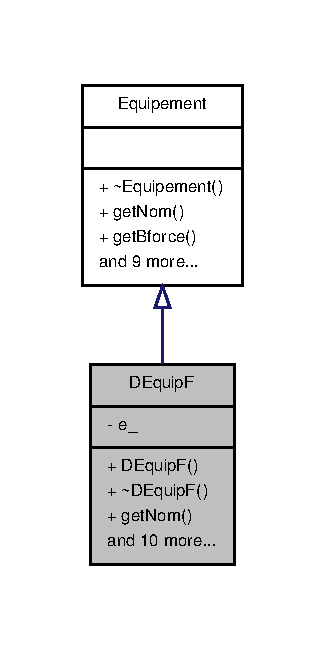
\includegraphics[width=156pt]{class_d_equip_f__inherit__graph}
\end{center}
\end{figure}


Graphe de collaboration de D\-Equip\-F\-:
\nopagebreak
\begin{figure}[H]
\begin{center}
\leavevmode
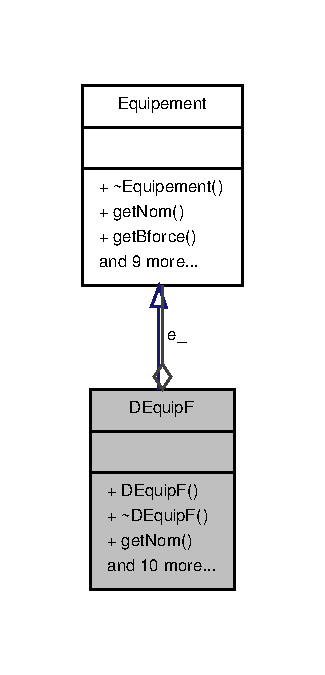
\includegraphics[width=156pt]{class_d_equip_f__coll__graph}
\end{center}
\end{figure}
\subsection*{Fonctions membres publiques}
\begin{DoxyCompactItemize}
\item 
\hypertarget{class_d_equip_f_a81f4d716356576692063657887a471d8}{{\bfseries D\-Equip\-F} (\hyperlink{class_equipement}{Equipement} $\ast$e)}\label{class_d_equip_f_a81f4d716356576692063657887a471d8}

\item 
int \hyperlink{class_d_equip_adb6645ce01c12a4cb3fe0b522ea6b25e}{get\-Bforce} ()
\begin{DoxyCompactList}\small\item\em Renvoie le bonus de force. \end{DoxyCompactList}\item 
int \hyperlink{class_d_equip_a085ea4ac21c238d8c147ff4e6d74794f}{get\-Bvie} ()
\begin{DoxyCompactList}\small\item\em Renvoie le bonus de vie. \end{DoxyCompactList}\item 
int \hyperlink{class_d_equip_a39407c92f0de87306a33f57fd22ce997}{get\-Bchance} ()
\begin{DoxyCompactList}\small\item\em Renvoie le bonus de chance. \end{DoxyCompactList}\item 
int \hyperlink{class_d_equip_a7b2c8227ae884c23ccc8f3a2e5702186}{get\-Armure} ()
\begin{DoxyCompactList}\small\item\em Renvoie le bonus d'armure. \end{DoxyCompactList}\item 
int \hyperlink{class_d_equip_a7c31f807517e5940e899780ac6d7a5c3}{type} ()
\begin{DoxyCompactList}\small\item\em Renvoie le type de l'\hyperlink{class_equipement}{Equipement}. \end{DoxyCompactList}\item 
virtual std\-::string \hyperlink{class_equipement_a0b0426a70bfce6e7c3efac605b75cd8e}{get\-Nom} ()
\begin{DoxyCompactList}\small\item\em Retourne le nom de l'equipement. \end{DoxyCompactList}\end{DoxyCompactItemize}
\subsection*{Fonctions membres protégées}
\begin{DoxyCompactItemize}
\item 
std\-::string \hyperlink{class_d_equip_af8a7e83f36094af1f34f5c81df6e3900}{replace} (std\-::string str)
\begin{DoxyCompactList}\small\item\em Retourne le nom de l'équipement modifié \end{DoxyCompactList}\end{DoxyCompactItemize}
\subsection*{Attributs protégés}
\begin{DoxyCompactItemize}
\item 
\hypertarget{class_d_equip_a0243fb57df463a3d0a7c57e6e7980210}{\hyperlink{class_equipement}{Equipement} $\ast$ \hyperlink{class_d_equip_a0243fb57df463a3d0a7c57e6e7980210}{e\-\_\-}}\label{class_d_equip_a0243fb57df463a3d0a7c57e6e7980210}

\begin{DoxyCompactList}\small\item\em \hyperlink{class_equipement}{Equipement} e pour la décoration. \end{DoxyCompactList}\item 
\hypertarget{class_equipement_a930290aac01ecd40c7a646ab8f66d742}{std\-::string {\bfseries nom\-\_\-}}\label{class_equipement_a930290aac01ecd40c7a646ab8f66d742}

\item 
\hypertarget{class_equipement_a69339ce4f1f5fe7e6fcdeda5b74c14a4}{int {\bfseries armure\-\_\-}}\label{class_equipement_a69339ce4f1f5fe7e6fcdeda5b74c14a4}

\item 
\hypertarget{class_equipement_aa70effa6a8144fe1f4fe874af7139793}{int {\bfseries bchance\-\_\-}}\label{class_equipement_aa70effa6a8144fe1f4fe874af7139793}

\item 
\hypertarget{class_equipement_a73ac5bff40e3f6bf1d8e6f0e524e750f}{int {\bfseries bvie\-\_\-}}\label{class_equipement_a73ac5bff40e3f6bf1d8e6f0e524e750f}

\item 
\hypertarget{class_equipement_af87cf3f291386d5401be6994dd8fb8be}{int {\bfseries bforce\-\_\-}}\label{class_equipement_af87cf3f291386d5401be6994dd8fb8be}

\end{DoxyCompactItemize}


\subsection{Description détaillée}
Decorator d'équipement de force , hérite de \hyperlink{class_d_equip}{D\-Equip}. 

\subsection{Documentation des fonctions membres}
\hypertarget{class_d_equip_a7b2c8227ae884c23ccc8f3a2e5702186}{\index{D\-Equip\-F@{D\-Equip\-F}!get\-Armure@{get\-Armure}}
\index{get\-Armure@{get\-Armure}!DEquipF@{D\-Equip\-F}}
\subsubsection[{get\-Armure}]{\setlength{\rightskip}{0pt plus 5cm}int D\-Equip\-::get\-Armure (
\begin{DoxyParamCaption}
{}
\end{DoxyParamCaption}
)\hspace{0.3cm}{\ttfamily [virtual]}, {\ttfamily [inherited]}}}\label{class_d_equip_a7b2c8227ae884c23ccc8f3a2e5702186}


Renvoie le bonus d'armure. 

\begin{DoxyReturn}{Renvoie}
armure Bonus d'armure 
\end{DoxyReturn}


Réimplémentée à partir de \hyperlink{class_equipement_a8577d49fd00b8effa39388feccb29901}{Equipement}.

\hypertarget{class_d_equip_a39407c92f0de87306a33f57fd22ce997}{\index{D\-Equip\-F@{D\-Equip\-F}!get\-Bchance@{get\-Bchance}}
\index{get\-Bchance@{get\-Bchance}!DEquipF@{D\-Equip\-F}}
\subsubsection[{get\-Bchance}]{\setlength{\rightskip}{0pt plus 5cm}int D\-Equip\-::get\-Bchance (
\begin{DoxyParamCaption}
{}
\end{DoxyParamCaption}
)\hspace{0.3cm}{\ttfamily [virtual]}, {\ttfamily [inherited]}}}\label{class_d_equip_a39407c92f0de87306a33f57fd22ce997}


Renvoie le bonus de chance. 

\begin{DoxyReturn}{Renvoie}
bchance Bonus de chance 
\end{DoxyReturn}


Réimplémentée à partir de \hyperlink{class_equipement_a73485135eacdf30d5f49c9e34e5f4d0e}{Equipement}.

\hypertarget{class_d_equip_adb6645ce01c12a4cb3fe0b522ea6b25e}{\index{D\-Equip\-F@{D\-Equip\-F}!get\-Bforce@{get\-Bforce}}
\index{get\-Bforce@{get\-Bforce}!DEquipF@{D\-Equip\-F}}
\subsubsection[{get\-Bforce}]{\setlength{\rightskip}{0pt plus 5cm}int D\-Equip\-::get\-Bforce (
\begin{DoxyParamCaption}
{}
\end{DoxyParamCaption}
)\hspace{0.3cm}{\ttfamily [virtual]}, {\ttfamily [inherited]}}}\label{class_d_equip_adb6645ce01c12a4cb3fe0b522ea6b25e}


Renvoie le bonus de force. 

\begin{DoxyReturn}{Renvoie}
bforce Bonus de force 
\end{DoxyReturn}


Réimplémentée à partir de \hyperlink{class_equipement_aabcf10fd762945fa4a37a9cf8321f463}{Equipement}.

\hypertarget{class_d_equip_a085ea4ac21c238d8c147ff4e6d74794f}{\index{D\-Equip\-F@{D\-Equip\-F}!get\-Bvie@{get\-Bvie}}
\index{get\-Bvie@{get\-Bvie}!DEquipF@{D\-Equip\-F}}
\subsubsection[{get\-Bvie}]{\setlength{\rightskip}{0pt plus 5cm}int D\-Equip\-::get\-Bvie (
\begin{DoxyParamCaption}
{}
\end{DoxyParamCaption}
)\hspace{0.3cm}{\ttfamily [virtual]}, {\ttfamily [inherited]}}}\label{class_d_equip_a085ea4ac21c238d8c147ff4e6d74794f}


Renvoie le bonus de vie. 

\begin{DoxyReturn}{Renvoie}
bvie Bonus de vie 
\end{DoxyReturn}


Réimplémentée à partir de \hyperlink{class_equipement_ad9fd7528c4f181970b7a0877f4145f89}{Equipement}.

\hypertarget{class_equipement_a0b0426a70bfce6e7c3efac605b75cd8e}{\index{D\-Equip\-F@{D\-Equip\-F}!get\-Nom@{get\-Nom}}
\index{get\-Nom@{get\-Nom}!DEquipF@{D\-Equip\-F}}
\subsubsection[{get\-Nom}]{\setlength{\rightskip}{0pt plus 5cm}std\-::string Equipement\-::get\-Nom (
\begin{DoxyParamCaption}
{}
\end{DoxyParamCaption}
)\hspace{0.3cm}{\ttfamily [virtual]}, {\ttfamily [inherited]}}}\label{class_equipement_a0b0426a70bfce6e7c3efac605b75cd8e}


Retourne le nom de l'equipement. 

\begin{DoxyReturn}{Renvoie}
Nom 
\end{DoxyReturn}
\hypertarget{class_d_equip_af8a7e83f36094af1f34f5c81df6e3900}{\index{D\-Equip\-F@{D\-Equip\-F}!replace@{replace}}
\index{replace@{replace}!DEquipF@{D\-Equip\-F}}
\subsubsection[{replace}]{\setlength{\rightskip}{0pt plus 5cm}std\-::string D\-Equip\-::replace (
\begin{DoxyParamCaption}
\item[{std\-::string}]{str}
\end{DoxyParamCaption}
)\hspace{0.3cm}{\ttfamily [protected]}, {\ttfamily [inherited]}}}\label{class_d_equip_af8a7e83f36094af1f34f5c81df6e3900}


Retourne le nom de l'équipement modifié 


\begin{DoxyParams}{Paramètres}
{\em Chaine} & de caractère à ajouter \\
\hline
\end{DoxyParams}
\begin{DoxyReturn}{Renvoie}
nom nom modifié 
\end{DoxyReturn}
\hypertarget{class_d_equip_a7c31f807517e5940e899780ac6d7a5c3}{\index{D\-Equip\-F@{D\-Equip\-F}!type@{type}}
\index{type@{type}!DEquipF@{D\-Equip\-F}}
\subsubsection[{type}]{\setlength{\rightskip}{0pt plus 5cm}int D\-Equip\-::type (
\begin{DoxyParamCaption}
{}
\end{DoxyParamCaption}
)\hspace{0.3cm}{\ttfamily [virtual]}, {\ttfamily [inherited]}}}\label{class_d_equip_a7c31f807517e5940e899780ac6d7a5c3}


Renvoie le type de l'\hyperlink{class_equipement}{Equipement}. 

\begin{DoxyReturn}{Renvoie}
entier type de l'\hyperlink{class_equipement}{Equipement} 
\end{DoxyReturn}


Implémente \hyperlink{class_equipement_a05b2c9d4cf22b6aefb6603fa4e322aa2}{Equipement}.


\hypertarget{class_d_equip_v}{\section{Référence de la classe D\-Equip\-V}
\label{class_d_equip_v}\index{D\-Equip\-V@{D\-Equip\-V}}
}


Decorator d'équipement de vie , hérite de \hyperlink{class_d_equip}{D\-Equip}.  




Graphe d'héritage de D\-Equip\-V\-:
\nopagebreak
\begin{figure}[H]
\begin{center}
\leavevmode
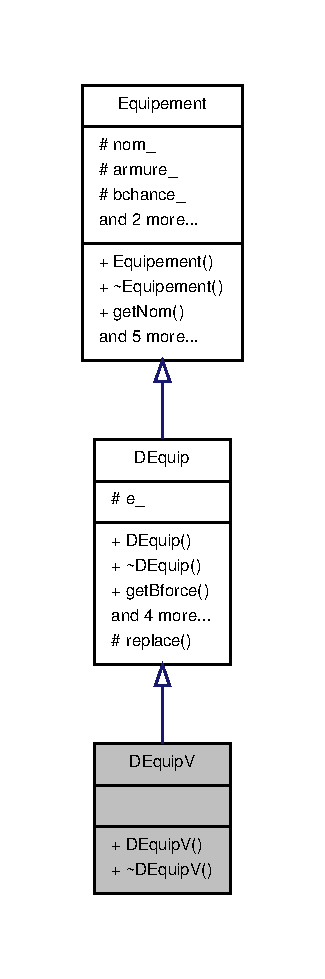
\includegraphics[width=156pt]{class_d_equip_v__inherit__graph}
\end{center}
\end{figure}


Graphe de collaboration de D\-Equip\-V\-:
\nopagebreak
\begin{figure}[H]
\begin{center}
\leavevmode
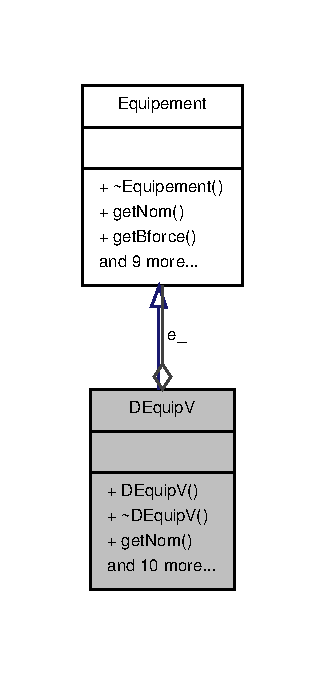
\includegraphics[width=156pt]{class_d_equip_v__coll__graph}
\end{center}
\end{figure}
\subsection*{Fonctions membres publiques}
\begin{DoxyCompactItemize}
\item 
\hypertarget{class_d_equip_v_acf6d9090ca81524f3c8118e4ff405416}{{\bfseries D\-Equip\-V} (\hyperlink{class_equipement}{Equipement} $\ast$e)}\label{class_d_equip_v_acf6d9090ca81524f3c8118e4ff405416}

\item 
int \hyperlink{class_d_equip_adb6645ce01c12a4cb3fe0b522ea6b25e}{get\-Bforce} ()
\begin{DoxyCompactList}\small\item\em Renvoie le bonus de force. \end{DoxyCompactList}\item 
int \hyperlink{class_d_equip_a085ea4ac21c238d8c147ff4e6d74794f}{get\-Bvie} ()
\begin{DoxyCompactList}\small\item\em Renvoie le bonus de vie. \end{DoxyCompactList}\item 
int \hyperlink{class_d_equip_a39407c92f0de87306a33f57fd22ce997}{get\-Bchance} ()
\begin{DoxyCompactList}\small\item\em Renvoie le bonus de chance. \end{DoxyCompactList}\item 
int \hyperlink{class_d_equip_a7b2c8227ae884c23ccc8f3a2e5702186}{get\-Armure} ()
\begin{DoxyCompactList}\small\item\em Renvoie le bonus d'armure. \end{DoxyCompactList}\item 
int \hyperlink{class_d_equip_a7c31f807517e5940e899780ac6d7a5c3}{type} ()
\begin{DoxyCompactList}\small\item\em Renvoie le type de l'\hyperlink{class_equipement}{Equipement}. \end{DoxyCompactList}\item 
virtual std\-::string \hyperlink{class_equipement_a0b0426a70bfce6e7c3efac605b75cd8e}{get\-Nom} ()
\begin{DoxyCompactList}\small\item\em Retourne le nom de l'equipement. \end{DoxyCompactList}\end{DoxyCompactItemize}
\subsection*{Fonctions membres protégées}
\begin{DoxyCompactItemize}
\item 
std\-::string \hyperlink{class_d_equip_af8a7e83f36094af1f34f5c81df6e3900}{replace} (std\-::string str)
\begin{DoxyCompactList}\small\item\em Retourne le nom de l'équipement modifié \end{DoxyCompactList}\end{DoxyCompactItemize}
\subsection*{Attributs protégés}
\begin{DoxyCompactItemize}
\item 
\hypertarget{class_d_equip_a0243fb57df463a3d0a7c57e6e7980210}{\hyperlink{class_equipement}{Equipement} $\ast$ \hyperlink{class_d_equip_a0243fb57df463a3d0a7c57e6e7980210}{e\-\_\-}}\label{class_d_equip_a0243fb57df463a3d0a7c57e6e7980210}

\begin{DoxyCompactList}\small\item\em \hyperlink{class_equipement}{Equipement} e pour la décoration. \end{DoxyCompactList}\item 
\hypertarget{class_equipement_a930290aac01ecd40c7a646ab8f66d742}{std\-::string {\bfseries nom\-\_\-}}\label{class_equipement_a930290aac01ecd40c7a646ab8f66d742}

\item 
\hypertarget{class_equipement_a69339ce4f1f5fe7e6fcdeda5b74c14a4}{int {\bfseries armure\-\_\-}}\label{class_equipement_a69339ce4f1f5fe7e6fcdeda5b74c14a4}

\item 
\hypertarget{class_equipement_aa70effa6a8144fe1f4fe874af7139793}{int {\bfseries bchance\-\_\-}}\label{class_equipement_aa70effa6a8144fe1f4fe874af7139793}

\item 
\hypertarget{class_equipement_a73ac5bff40e3f6bf1d8e6f0e524e750f}{int {\bfseries bvie\-\_\-}}\label{class_equipement_a73ac5bff40e3f6bf1d8e6f0e524e750f}

\item 
\hypertarget{class_equipement_af87cf3f291386d5401be6994dd8fb8be}{int {\bfseries bforce\-\_\-}}\label{class_equipement_af87cf3f291386d5401be6994dd8fb8be}

\end{DoxyCompactItemize}


\subsection{Description détaillée}
Decorator d'équipement de vie , hérite de \hyperlink{class_d_equip}{D\-Equip}. 

\subsection{Documentation des fonctions membres}
\hypertarget{class_d_equip_a7b2c8227ae884c23ccc8f3a2e5702186}{\index{D\-Equip\-V@{D\-Equip\-V}!get\-Armure@{get\-Armure}}
\index{get\-Armure@{get\-Armure}!DEquipV@{D\-Equip\-V}}
\subsubsection[{get\-Armure}]{\setlength{\rightskip}{0pt plus 5cm}int D\-Equip\-::get\-Armure (
\begin{DoxyParamCaption}
{}
\end{DoxyParamCaption}
)\hspace{0.3cm}{\ttfamily [virtual]}, {\ttfamily [inherited]}}}\label{class_d_equip_a7b2c8227ae884c23ccc8f3a2e5702186}


Renvoie le bonus d'armure. 

\begin{DoxyReturn}{Renvoie}
armure Bonus d'armure 
\end{DoxyReturn}


Réimplémentée à partir de \hyperlink{class_equipement_a8577d49fd00b8effa39388feccb29901}{Equipement}.

\hypertarget{class_d_equip_a39407c92f0de87306a33f57fd22ce997}{\index{D\-Equip\-V@{D\-Equip\-V}!get\-Bchance@{get\-Bchance}}
\index{get\-Bchance@{get\-Bchance}!DEquipV@{D\-Equip\-V}}
\subsubsection[{get\-Bchance}]{\setlength{\rightskip}{0pt plus 5cm}int D\-Equip\-::get\-Bchance (
\begin{DoxyParamCaption}
{}
\end{DoxyParamCaption}
)\hspace{0.3cm}{\ttfamily [virtual]}, {\ttfamily [inherited]}}}\label{class_d_equip_a39407c92f0de87306a33f57fd22ce997}


Renvoie le bonus de chance. 

\begin{DoxyReturn}{Renvoie}
bchance Bonus de chance 
\end{DoxyReturn}


Réimplémentée à partir de \hyperlink{class_equipement_a73485135eacdf30d5f49c9e34e5f4d0e}{Equipement}.

\hypertarget{class_d_equip_adb6645ce01c12a4cb3fe0b522ea6b25e}{\index{D\-Equip\-V@{D\-Equip\-V}!get\-Bforce@{get\-Bforce}}
\index{get\-Bforce@{get\-Bforce}!DEquipV@{D\-Equip\-V}}
\subsubsection[{get\-Bforce}]{\setlength{\rightskip}{0pt plus 5cm}int D\-Equip\-::get\-Bforce (
\begin{DoxyParamCaption}
{}
\end{DoxyParamCaption}
)\hspace{0.3cm}{\ttfamily [virtual]}, {\ttfamily [inherited]}}}\label{class_d_equip_adb6645ce01c12a4cb3fe0b522ea6b25e}


Renvoie le bonus de force. 

\begin{DoxyReturn}{Renvoie}
bforce Bonus de force 
\end{DoxyReturn}


Réimplémentée à partir de \hyperlink{class_equipement_aabcf10fd762945fa4a37a9cf8321f463}{Equipement}.

\hypertarget{class_d_equip_a085ea4ac21c238d8c147ff4e6d74794f}{\index{D\-Equip\-V@{D\-Equip\-V}!get\-Bvie@{get\-Bvie}}
\index{get\-Bvie@{get\-Bvie}!DEquipV@{D\-Equip\-V}}
\subsubsection[{get\-Bvie}]{\setlength{\rightskip}{0pt plus 5cm}int D\-Equip\-::get\-Bvie (
\begin{DoxyParamCaption}
{}
\end{DoxyParamCaption}
)\hspace{0.3cm}{\ttfamily [virtual]}, {\ttfamily [inherited]}}}\label{class_d_equip_a085ea4ac21c238d8c147ff4e6d74794f}


Renvoie le bonus de vie. 

\begin{DoxyReturn}{Renvoie}
bvie Bonus de vie 
\end{DoxyReturn}


Réimplémentée à partir de \hyperlink{class_equipement_ad9fd7528c4f181970b7a0877f4145f89}{Equipement}.

\hypertarget{class_equipement_a0b0426a70bfce6e7c3efac605b75cd8e}{\index{D\-Equip\-V@{D\-Equip\-V}!get\-Nom@{get\-Nom}}
\index{get\-Nom@{get\-Nom}!DEquipV@{D\-Equip\-V}}
\subsubsection[{get\-Nom}]{\setlength{\rightskip}{0pt plus 5cm}std\-::string Equipement\-::get\-Nom (
\begin{DoxyParamCaption}
{}
\end{DoxyParamCaption}
)\hspace{0.3cm}{\ttfamily [virtual]}, {\ttfamily [inherited]}}}\label{class_equipement_a0b0426a70bfce6e7c3efac605b75cd8e}


Retourne le nom de l'equipement. 

\begin{DoxyReturn}{Renvoie}
Nom 
\end{DoxyReturn}
\hypertarget{class_d_equip_af8a7e83f36094af1f34f5c81df6e3900}{\index{D\-Equip\-V@{D\-Equip\-V}!replace@{replace}}
\index{replace@{replace}!DEquipV@{D\-Equip\-V}}
\subsubsection[{replace}]{\setlength{\rightskip}{0pt plus 5cm}std\-::string D\-Equip\-::replace (
\begin{DoxyParamCaption}
\item[{std\-::string}]{str}
\end{DoxyParamCaption}
)\hspace{0.3cm}{\ttfamily [protected]}, {\ttfamily [inherited]}}}\label{class_d_equip_af8a7e83f36094af1f34f5c81df6e3900}


Retourne le nom de l'équipement modifié 


\begin{DoxyParams}{Paramètres}
{\em Chaine} & de caractère à ajouter \\
\hline
\end{DoxyParams}
\begin{DoxyReturn}{Renvoie}
nom nom modifié 
\end{DoxyReturn}
\hypertarget{class_d_equip_a7c31f807517e5940e899780ac6d7a5c3}{\index{D\-Equip\-V@{D\-Equip\-V}!type@{type}}
\index{type@{type}!DEquipV@{D\-Equip\-V}}
\subsubsection[{type}]{\setlength{\rightskip}{0pt plus 5cm}int D\-Equip\-::type (
\begin{DoxyParamCaption}
{}
\end{DoxyParamCaption}
)\hspace{0.3cm}{\ttfamily [virtual]}, {\ttfamily [inherited]}}}\label{class_d_equip_a7c31f807517e5940e899780ac6d7a5c3}


Renvoie le type de l'\hyperlink{class_equipement}{Equipement}. 

\begin{DoxyReturn}{Renvoie}
entier type de l'\hyperlink{class_equipement}{Equipement} 
\end{DoxyReturn}


Implémente \hyperlink{class_equipement_a05b2c9d4cf22b6aefb6603fa4e322aa2}{Equipement}.


\hypertarget{class_empty_room}{\section{Référence de la classe Empty\-Room}
\label{class_empty_room}\index{Empty\-Room@{Empty\-Room}}
}


Salle vide.  




Graphe d'héritage de Empty\-Room\-:
\nopagebreak
\begin{figure}[H]
\begin{center}
\leavevmode
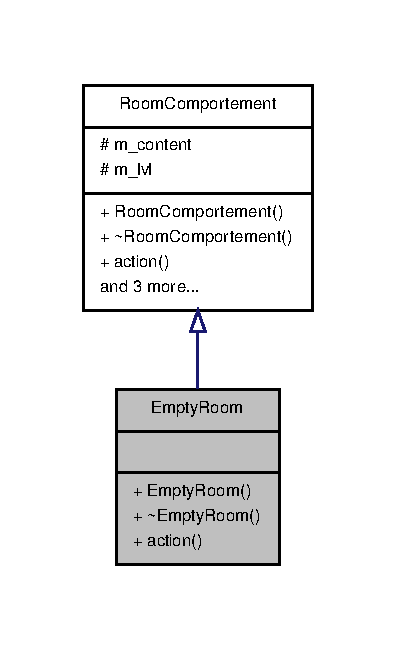
\includegraphics[width=190pt]{class_empty_room__inherit__graph}
\end{center}
\end{figure}


Graphe de collaboration de Empty\-Room\-:
\nopagebreak
\begin{figure}[H]
\begin{center}
\leavevmode
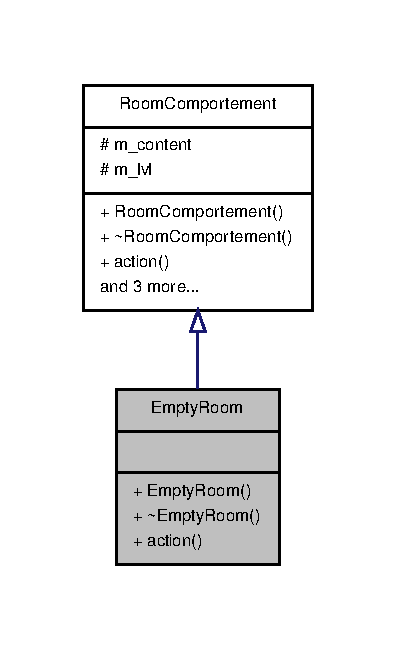
\includegraphics[width=190pt]{class_empty_room__coll__graph}
\end{center}
\end{figure}
\subsection*{Fonctions membres publiques}
\begin{DoxyCompactItemize}
\item 
\hypertarget{class_empty_room_adff09606225e39899242059db5d8e64e}{{\bfseries Empty\-Room} (int lvl=0)}\label{class_empty_room_adff09606225e39899242059db5d8e64e}

\item 
virtual int \hyperlink{class_empty_room_a31fdcab2da18636773d28f393e48cd7b}{action} (\hyperlink{class_personnage}{Personnage} \&perso)
\begin{DoxyCompactList}\small\item\em Redonne un petit peu de points de vie au joueur. \end{DoxyCompactList}\item 
virtual bool \hyperlink{class_room_comportement_a240991f90b07c35e0e9114e6a203ba88}{is\-End} () const 
\begin{DoxyCompactList}\small\item\em Vérifie la fin. \end{DoxyCompactList}\item 
int \hyperlink{class_room_comportement_a645473f228c0e73532a309ad512456eb}{get\-Lvl} ()
\begin{DoxyCompactList}\small\item\em Récupère le niveau ou force de la salle. \end{DoxyCompactList}\item 
std\-::string \hyperlink{class_room_comportement_a6927d638d17858a303d77b449c7552b4}{get\-Content} ()
\begin{DoxyCompactList}\small\item\em Récupère le contenue de la salle. \end{DoxyCompactList}\end{DoxyCompactItemize}
\subsection*{Attributs protégés}
\begin{DoxyCompactItemize}
\item 
\hypertarget{class_room_comportement_a48186371372d14465faffc7734e89fdc}{std\-::string \hyperlink{class_room_comportement_a48186371372d14465faffc7734e89fdc}{m\-\_\-content}}\label{class_room_comportement_a48186371372d14465faffc7734e89fdc}

\begin{DoxyCompactList}\small\item\em Valeur du contenue a afficher. \end{DoxyCompactList}\item 
\hypertarget{class_room_comportement_acfc0d0c3c7dbcd88235e8c615f7290a3}{int \hyperlink{class_room_comportement_acfc0d0c3c7dbcd88235e8c615f7290a3}{m\-\_\-lvl}}\label{class_room_comportement_acfc0d0c3c7dbcd88235e8c615f7290a3}

\begin{DoxyCompactList}\small\item\em stock le niveau de la salle \end{DoxyCompactList}\end{DoxyCompactItemize}


\subsection{Description détaillée}
Salle vide. 

l'action ne fait rien 

\subsection{Documentation des fonctions membres}
\hypertarget{class_empty_room_a31fdcab2da18636773d28f393e48cd7b}{\index{Empty\-Room@{Empty\-Room}!action@{action}}
\index{action@{action}!EmptyRoom@{Empty\-Room}}
\subsubsection[{action}]{\setlength{\rightskip}{0pt plus 5cm}int Empty\-Room\-::action (
\begin{DoxyParamCaption}
\item[{{\bf Personnage} \&}]{perso}
\end{DoxyParamCaption}
)\hspace{0.3cm}{\ttfamily [virtual]}}}\label{class_empty_room_a31fdcab2da18636773d28f393e48cd7b}


Redonne un petit peu de points de vie au joueur. 


\begin{DoxyParams}{Paramètres}
{\em perso} & \\
\hline
\end{DoxyParams}
\begin{DoxyReturn}{Renvoie}

\end{DoxyReturn}


Implémente \hyperlink{class_room_comportement_ac5b509f405f9e52fea3a9392210fbbdb}{Room\-Comportement}.

\hypertarget{class_room_comportement_a6927d638d17858a303d77b449c7552b4}{\index{Empty\-Room@{Empty\-Room}!get\-Content@{get\-Content}}
\index{get\-Content@{get\-Content}!EmptyRoom@{Empty\-Room}}
\subsubsection[{get\-Content}]{\setlength{\rightskip}{0pt plus 5cm}std\-::string Room\-Comportement\-::get\-Content (
\begin{DoxyParamCaption}
{}
\end{DoxyParamCaption}
)\hspace{0.3cm}{\ttfamily [inherited]}}}\label{class_room_comportement_a6927d638d17858a303d77b449c7552b4}


Récupère le contenue de la salle. 

\begin{DoxyReturn}{Renvoie}
contenue de la salle 
\end{DoxyReturn}
\hypertarget{class_room_comportement_a645473f228c0e73532a309ad512456eb}{\index{Empty\-Room@{Empty\-Room}!get\-Lvl@{get\-Lvl}}
\index{get\-Lvl@{get\-Lvl}!EmptyRoom@{Empty\-Room}}
\subsubsection[{get\-Lvl}]{\setlength{\rightskip}{0pt plus 5cm}int Room\-Comportement\-::get\-Lvl (
\begin{DoxyParamCaption}
{}
\end{DoxyParamCaption}
)\hspace{0.3cm}{\ttfamily [inherited]}}}\label{class_room_comportement_a645473f228c0e73532a309ad512456eb}


Récupère le niveau ou force de la salle. 

\begin{DoxyReturn}{Renvoie}
le niveau 
\end{DoxyReturn}
\hypertarget{class_room_comportement_a240991f90b07c35e0e9114e6a203ba88}{\index{Empty\-Room@{Empty\-Room}!is\-End@{is\-End}}
\index{is\-End@{is\-End}!EmptyRoom@{Empty\-Room}}
\subsubsection[{is\-End}]{\setlength{\rightskip}{0pt plus 5cm}bool Room\-Comportement\-::is\-End (
\begin{DoxyParamCaption}
{}
\end{DoxyParamCaption}
) const\hspace{0.3cm}{\ttfamily [virtual]}, {\ttfamily [inherited]}}}\label{class_room_comportement_a240991f90b07c35e0e9114e6a203ba88}


Vérifie la fin. 

\begin{DoxyReturn}{Renvoie}
vrais si on est sur la salle de fin 
\end{DoxyReturn}


Réimplémentée dans \hyperlink{class_end_room_a357ab3e12cd3af4e373a8d7c8c4681f4}{End\-Room}.


\section{Référence de la classe End\-Room}
\label{class_end_room}\index{End\-Room@{End\-Room}}


Salle de fin du labyrinth.  




Graphe d'héritage de End\-Room\-:\nopagebreak
\begin{figure}[H]
\begin{center}
\leavevmode
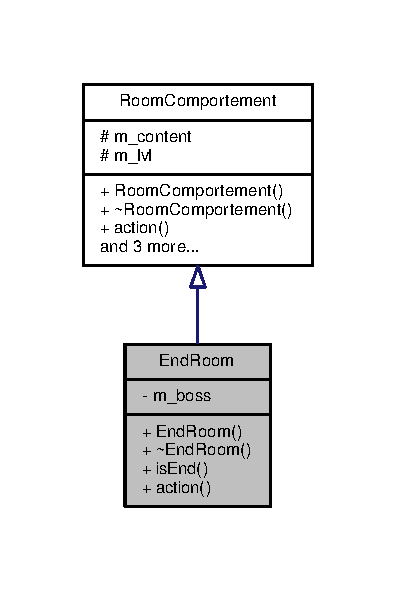
\includegraphics[width=190pt]{class_end_room__inherit__graph}
\end{center}
\end{figure}


Graphe de collaboration de End\-Room\-:\nopagebreak
\begin{figure}[H]
\begin{center}
\leavevmode
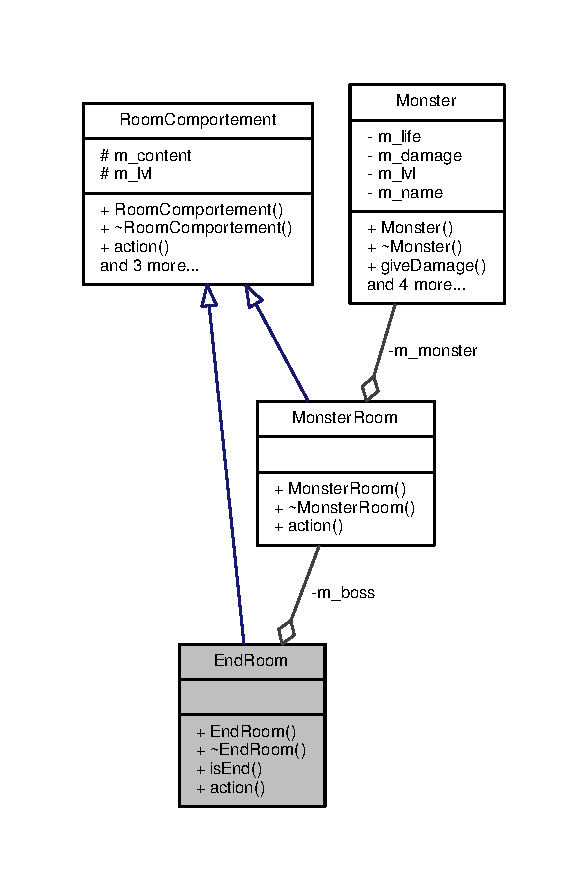
\includegraphics[width=282pt]{class_end_room__coll__graph}
\end{center}
\end{figure}
\subsection*{Fonctions membres publiques}
\begin{DoxyCompactItemize}
\item 
{\bf End\-Room} (int lvl=10)
\item 
virtual {\bf $\sim$\-End\-Room} ()
\item 
virtual bool {\bf is\-End} () const 
\begin{DoxyCompactList}\small\item\em Vérifie la fin. \end{DoxyCompactList}\item 
virtual int {\bf action} ({\bf Personnage} \&perso)
\begin{DoxyCompactList}\small\item\em Combat un boss puis fini le jeu. \end{DoxyCompactList}\item 
int {\bf get\-Lvl} ()
\begin{DoxyCompactList}\small\item\em Récupère le niveau ou force de la salle. \end{DoxyCompactList}\item 
std\-::string {\bf get\-Content} ()
\begin{DoxyCompactList}\small\item\em Récupère le contenue de la salle. \end{DoxyCompactList}\end{DoxyCompactItemize}
\subsection*{Attributs protégés}
\begin{DoxyCompactItemize}
\item 
std\-::string {\bf m\-\_\-content}
\begin{DoxyCompactList}\small\item\em Valeur du contenue a afficher. \end{DoxyCompactList}\item 
int {\bf m\-\_\-lvl}
\begin{DoxyCompactList}\small\item\em stock le niveau de la salle \end{DoxyCompactList}\end{DoxyCompactItemize}
\subsection*{Attributs privés}
\begin{DoxyCompactItemize}
\item 
{\bf Monster\-Room} {\bf m\-\_\-boss}
\begin{DoxyCompactList}\small\item\em utilise un comportement \doxyref{Monster\-Room}{p.}{class_monster_room} pour faire un combat \end{DoxyCompactList}\end{DoxyCompactItemize}


\subsection{Description détaillée}
Salle de fin du labyrinth. 

\subsection{Documentation des constructeurs et destructeur}
\index{End\-Room@{End\-Room}!End\-Room@{End\-Room}}
\index{End\-Room@{End\-Room}!EndRoom@{End\-Room}}
\subsubsection[{End\-Room}]{\setlength{\rightskip}{0pt plus 5cm}End\-Room\-::\-End\-Room (
\begin{DoxyParamCaption}
\item[{int}]{lvl = {\ttfamily 10}}
\end{DoxyParamCaption}
)}\label{class_end_room_aab637ba35afa1f07cf888cd48714809f}
\index{End\-Room@{End\-Room}!$\sim$\-End\-Room@{$\sim$\-End\-Room}}
\index{$\sim$\-End\-Room@{$\sim$\-End\-Room}!EndRoom@{End\-Room}}
\subsubsection[{$\sim$\-End\-Room}]{\setlength{\rightskip}{0pt plus 5cm}End\-Room\-::$\sim$\-End\-Room (
\begin{DoxyParamCaption}
{}
\end{DoxyParamCaption}
)\hspace{0.3cm}{\ttfamily [virtual]}}\label{class_end_room_afecb4fdaec217d7a8af9210769075efe}


\subsection{Documentation des fonctions membres}
\index{End\-Room@{End\-Room}!action@{action}}
\index{action@{action}!EndRoom@{End\-Room}}
\subsubsection[{action}]{\setlength{\rightskip}{0pt plus 5cm}int End\-Room\-::action (
\begin{DoxyParamCaption}
\item[{{\bf Personnage} \&}]{perso}
\end{DoxyParamCaption}
)\hspace{0.3cm}{\ttfamily [virtual]}}\label{class_end_room_ad7691b55dcf3ed863c8a774138105900}


Combat un boss puis fini le jeu. 

La fin est obligatoire, soit le joueur tue le boss et gagne, soit il meurt et perd.


\begin{DoxyParams}{Paramètres}
{\em perso} & \doxyref{Personnage}{p.}{class_personnage} qui l'éxecute\\
\hline
\end{DoxyParams}
\begin{DoxyReturn}{Renvoie}
l'action realisé 
\end{DoxyReturn}


Implémente {\bf Room\-Comportement} \doxyref{}{p.}{class_room_comportement_ac5b509f405f9e52fea3a9392210fbbdb}.

\index{End\-Room@{End\-Room}!get\-Content@{get\-Content}}
\index{get\-Content@{get\-Content}!EndRoom@{End\-Room}}
\subsubsection[{get\-Content}]{\setlength{\rightskip}{0pt plus 5cm}std\-::string Room\-Comportement\-::get\-Content (
\begin{DoxyParamCaption}
{}
\end{DoxyParamCaption}
)\hspace{0.3cm}{\ttfamily [inherited]}}\label{class_room_comportement_a6927d638d17858a303d77b449c7552b4}


Récupère le contenue de la salle. 

\begin{DoxyReturn}{Renvoie}
contenue de la salle 
\end{DoxyReturn}
\index{End\-Room@{End\-Room}!get\-Lvl@{get\-Lvl}}
\index{get\-Lvl@{get\-Lvl}!EndRoom@{End\-Room}}
\subsubsection[{get\-Lvl}]{\setlength{\rightskip}{0pt plus 5cm}int Room\-Comportement\-::get\-Lvl (
\begin{DoxyParamCaption}
{}
\end{DoxyParamCaption}
)\hspace{0.3cm}{\ttfamily [inherited]}}\label{class_room_comportement_a645473f228c0e73532a309ad512456eb}


Récupère le niveau ou force de la salle. 

\begin{DoxyReturn}{Renvoie}
le niveau 
\end{DoxyReturn}
\index{End\-Room@{End\-Room}!is\-End@{is\-End}}
\index{is\-End@{is\-End}!EndRoom@{End\-Room}}
\subsubsection[{is\-End}]{\setlength{\rightskip}{0pt plus 5cm}bool End\-Room\-::is\-End (
\begin{DoxyParamCaption}
{}
\end{DoxyParamCaption}
) const\hspace{0.3cm}{\ttfamily [virtual]}}\label{class_end_room_a357ab3e12cd3af4e373a8d7c8c4681f4}


Vérifie la fin. 

\begin{DoxyReturn}{Renvoie}
vrais si on est sur la salle de fin 
\end{DoxyReturn}


Réimplémentée à partir de {\bf Room\-Comportement} \doxyref{}{p.}{class_room_comportement_a240991f90b07c35e0e9114e6a203ba88}.



\subsection{Documentation des données membres}
\index{End\-Room@{End\-Room}!m\-\_\-boss@{m\-\_\-boss}}
\index{m\-\_\-boss@{m\-\_\-boss}!EndRoom@{End\-Room}}
\subsubsection[{m\-\_\-boss}]{\setlength{\rightskip}{0pt plus 5cm}{\bf Monster\-Room} End\-Room\-::m\-\_\-boss\hspace{0.3cm}{\ttfamily [private]}}\label{class_end_room_abcccd9156525db2da6d47667969a041f}


utilise un comportement \doxyref{Monster\-Room}{p.}{class_monster_room} pour faire un combat 

\index{End\-Room@{End\-Room}!m\-\_\-content@{m\-\_\-content}}
\index{m\-\_\-content@{m\-\_\-content}!EndRoom@{End\-Room}}
\subsubsection[{m\-\_\-content}]{\setlength{\rightskip}{0pt plus 5cm}std\-::string Room\-Comportement\-::m\-\_\-content\hspace{0.3cm}{\ttfamily [protected]}, {\ttfamily [inherited]}}\label{class_room_comportement_a48186371372d14465faffc7734e89fdc}


Valeur du contenue a afficher. 

\index{End\-Room@{End\-Room}!m\-\_\-lvl@{m\-\_\-lvl}}
\index{m\-\_\-lvl@{m\-\_\-lvl}!EndRoom@{End\-Room}}
\subsubsection[{m\-\_\-lvl}]{\setlength{\rightskip}{0pt plus 5cm}int Room\-Comportement\-::m\-\_\-lvl\hspace{0.3cm}{\ttfamily [protected]}, {\ttfamily [inherited]}}\label{class_room_comportement_acfc0d0c3c7dbcd88235e8c615f7290a3}


stock le niveau de la salle 



La documentation de cette classe a été générée à partir des fichiers suivants \-:\begin{DoxyCompactItemize}
\item 
src/{\bf End\-Room.\-hpp}\item 
src/{\bf End\-Room.\-cpp}\end{DoxyCompactItemize}

\section{Référence de la classe Epee}
\label{class_epee}\index{Epee@{Epee}}


\doxyref{Epee}{p.}{class_epee} herite de \doxyref{Arme}{p.}{class_arme}.  




Graphe d'héritage de Epee\-:\nopagebreak
\begin{figure}[H]
\begin{center}
\leavevmode
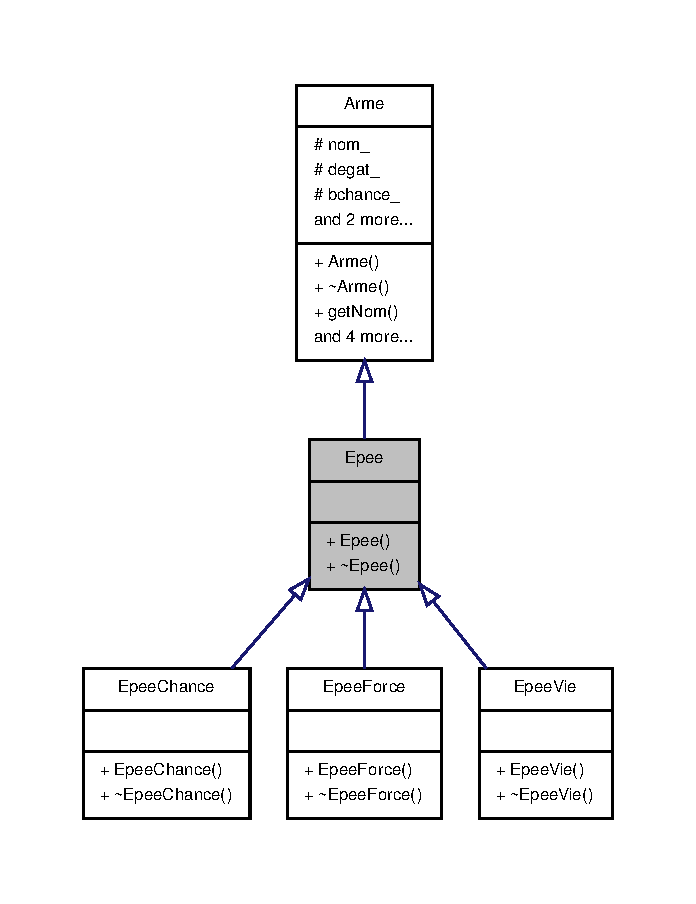
\includegraphics[width=334pt]{class_epee__inherit__graph}
\end{center}
\end{figure}


Graphe de collaboration de Epee\-:\nopagebreak
\begin{figure}[H]
\begin{center}
\leavevmode
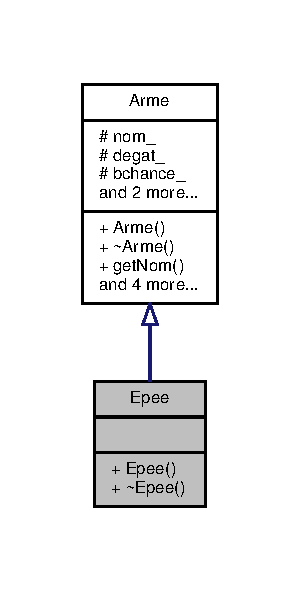
\includegraphics[width=144pt]{class_epee__coll__graph}
\end{center}
\end{figure}
\subsection*{Fonctions membres publiques}
\begin{DoxyCompactItemize}
\item 
{\bf Epee} ()
\item 
virtual {\bf $\sim$\-Epee} ()
\item 
virtual std\-::string {\bf get\-Nom} ()
\begin{DoxyCompactList}\small\item\em Retourne le nom de l'arme. \end{DoxyCompactList}\item 
virtual int {\bf get\-Bforce} ()
\begin{DoxyCompactList}\small\item\em Retourne le bonus de force. \end{DoxyCompactList}\item 
virtual int {\bf get\-Bvie} ()
\begin{DoxyCompactList}\small\item\em Retourne le bonus de vie. \end{DoxyCompactList}\item 
virtual int {\bf get\-Bchance} ()
\begin{DoxyCompactList}\small\item\em Retourne le bonus de chance. \end{DoxyCompactList}\item 
virtual int {\bf get\-Degat} ()
\begin{DoxyCompactList}\small\item\em Retourne les degats de l'arme. \end{DoxyCompactList}\end{DoxyCompactItemize}
\subsection*{Attributs protégés}
\begin{DoxyCompactItemize}
\item 
std\-::string {\bf nom\-\_\-}
\begin{DoxyCompactList}\small\item\em Nom de l'arme. \end{DoxyCompactList}\item 
int {\bf degat\-\_\-}
\begin{DoxyCompactList}\small\item\em Bonus de dégat. \end{DoxyCompactList}\item 
int {\bf bchance\-\_\-}
\begin{DoxyCompactList}\small\item\em Bonus de chance. \end{DoxyCompactList}\item 
int {\bf bvie\-\_\-}
\begin{DoxyCompactList}\small\item\em Bonus de vie. \end{DoxyCompactList}\item 
int {\bf bforce\-\_\-}
\begin{DoxyCompactList}\small\item\em Bonus de force. \end{DoxyCompactList}\end{DoxyCompactItemize}


\subsection{Description détaillée}
\doxyref{Epee}{p.}{class_epee} herite de \doxyref{Arme}{p.}{class_arme}. 

\subsection{Documentation des constructeurs et destructeur}
\index{Epee@{Epee}!Epee@{Epee}}
\index{Epee@{Epee}!Epee@{Epee}}
\subsubsection[{Epee}]{\setlength{\rightskip}{0pt plus 5cm}Epee\-::\-Epee (
\begin{DoxyParamCaption}
{}
\end{DoxyParamCaption}
)}\label{class_epee_ae61b96df89077d64e5578d1077220e75}
\index{Epee@{Epee}!$\sim$\-Epee@{$\sim$\-Epee}}
\index{$\sim$\-Epee@{$\sim$\-Epee}!Epee@{Epee}}
\subsubsection[{$\sim$\-Epee}]{\setlength{\rightskip}{0pt plus 5cm}Epee\-::$\sim$\-Epee (
\begin{DoxyParamCaption}
{}
\end{DoxyParamCaption}
)\hspace{0.3cm}{\ttfamily [virtual]}}\label{class_epee_ad58317e87c3d7eed03c7378a1b76afd4}


\subsection{Documentation des fonctions membres}
\index{Epee@{Epee}!get\-Bchance@{get\-Bchance}}
\index{get\-Bchance@{get\-Bchance}!Epee@{Epee}}
\subsubsection[{get\-Bchance}]{\setlength{\rightskip}{0pt plus 5cm}int Arme\-::get\-Bchance (
\begin{DoxyParamCaption}
{}
\end{DoxyParamCaption}
)\hspace{0.3cm}{\ttfamily [virtual]}, {\ttfamily [inherited]}}\label{class_arme_a6cb83d15008174152e424bebd0921069}


Retourne le bonus de chance. 

\begin{DoxyReturn}{Renvoie}
Bchance 
\end{DoxyReturn}


Réimplémentée dans {\bf D\-Arme} \doxyref{}{p.}{class_d_arme_ad50d376b08d62276b7cf50d2cd59d619}.

\index{Epee@{Epee}!get\-Bforce@{get\-Bforce}}
\index{get\-Bforce@{get\-Bforce}!Epee@{Epee}}
\subsubsection[{get\-Bforce}]{\setlength{\rightskip}{0pt plus 5cm}int Arme\-::get\-Bforce (
\begin{DoxyParamCaption}
{}
\end{DoxyParamCaption}
)\hspace{0.3cm}{\ttfamily [virtual]}, {\ttfamily [inherited]}}\label{class_arme_a3939e914a9ccc898de76db26bc8c24e7}


Retourne le bonus de force. 

\begin{DoxyReturn}{Renvoie}
Bforce 
\end{DoxyReturn}


Réimplémentée dans {\bf D\-Arme} \doxyref{}{p.}{class_d_arme_a76075bcbe61b20bd0e21e2d06fe33ab7}.

\index{Epee@{Epee}!get\-Bvie@{get\-Bvie}}
\index{get\-Bvie@{get\-Bvie}!Epee@{Epee}}
\subsubsection[{get\-Bvie}]{\setlength{\rightskip}{0pt plus 5cm}int Arme\-::get\-Bvie (
\begin{DoxyParamCaption}
{}
\end{DoxyParamCaption}
)\hspace{0.3cm}{\ttfamily [virtual]}, {\ttfamily [inherited]}}\label{class_arme_a479453fea0d6789e34ccaf193b3098ce}


Retourne le bonus de vie. 

\begin{DoxyReturn}{Renvoie}
Bvie 
\end{DoxyReturn}


Réimplémentée dans {\bf D\-Arme} \doxyref{}{p.}{class_d_arme_a91b3a3100969a568a8408ba098668398}.

\index{Epee@{Epee}!get\-Degat@{get\-Degat}}
\index{get\-Degat@{get\-Degat}!Epee@{Epee}}
\subsubsection[{get\-Degat}]{\setlength{\rightskip}{0pt plus 5cm}int Arme\-::get\-Degat (
\begin{DoxyParamCaption}
{}
\end{DoxyParamCaption}
)\hspace{0.3cm}{\ttfamily [virtual]}, {\ttfamily [inherited]}}\label{class_arme_a06ced3532b0e60cc900674a94c0cf29b}


Retourne les degats de l'arme. 

\begin{DoxyReturn}{Renvoie}
degats 
\end{DoxyReturn}


Réimplémentée dans {\bf D\-Arme} \doxyref{}{p.}{class_d_arme_a7396e865674067f4f21a28e6babc0fad}.

\index{Epee@{Epee}!get\-Nom@{get\-Nom}}
\index{get\-Nom@{get\-Nom}!Epee@{Epee}}
\subsubsection[{get\-Nom}]{\setlength{\rightskip}{0pt plus 5cm}std\-::string Arme\-::get\-Nom (
\begin{DoxyParamCaption}
{}
\end{DoxyParamCaption}
)\hspace{0.3cm}{\ttfamily [virtual]}, {\ttfamily [inherited]}}\label{class_arme_ab1b18cfa41fac19fccedf2165b9ff33c}


Retourne le nom de l'arme. 

\begin{DoxyReturn}{Renvoie}
Nom 
\end{DoxyReturn}


\subsection{Documentation des données membres}
\index{Epee@{Epee}!bchance\-\_\-@{bchance\-\_\-}}
\index{bchance\-\_\-@{bchance\-\_\-}!Epee@{Epee}}
\subsubsection[{bchance\-\_\-}]{\setlength{\rightskip}{0pt plus 5cm}int Arme\-::bchance\-\_\-\hspace{0.3cm}{\ttfamily [protected]}, {\ttfamily [inherited]}}\label{class_arme_a688792d4393f9e690aa103a8e68c541c}


Bonus de chance. 

\index{Epee@{Epee}!bforce\-\_\-@{bforce\-\_\-}}
\index{bforce\-\_\-@{bforce\-\_\-}!Epee@{Epee}}
\subsubsection[{bforce\-\_\-}]{\setlength{\rightskip}{0pt plus 5cm}int Arme\-::bforce\-\_\-\hspace{0.3cm}{\ttfamily [protected]}, {\ttfamily [inherited]}}\label{class_arme_a779e9838aa9c50d948f58b593fc5954b}


Bonus de force. 

\index{Epee@{Epee}!bvie\-\_\-@{bvie\-\_\-}}
\index{bvie\-\_\-@{bvie\-\_\-}!Epee@{Epee}}
\subsubsection[{bvie\-\_\-}]{\setlength{\rightskip}{0pt plus 5cm}int Arme\-::bvie\-\_\-\hspace{0.3cm}{\ttfamily [protected]}, {\ttfamily [inherited]}}\label{class_arme_a4606c075b38ef49f6ed2ed06d6185173}


Bonus de vie. 

\index{Epee@{Epee}!degat\-\_\-@{degat\-\_\-}}
\index{degat\-\_\-@{degat\-\_\-}!Epee@{Epee}}
\subsubsection[{degat\-\_\-}]{\setlength{\rightskip}{0pt plus 5cm}int Arme\-::degat\-\_\-\hspace{0.3cm}{\ttfamily [protected]}, {\ttfamily [inherited]}}\label{class_arme_a15f99a8b95c2d6f5beb9f473df79e399}


Bonus de dégat. 

\index{Epee@{Epee}!nom\-\_\-@{nom\-\_\-}}
\index{nom\-\_\-@{nom\-\_\-}!Epee@{Epee}}
\subsubsection[{nom\-\_\-}]{\setlength{\rightskip}{0pt plus 5cm}std\-::string Arme\-::nom\-\_\-\hspace{0.3cm}{\ttfamily [protected]}, {\ttfamily [inherited]}}\label{class_arme_a347394a5ab5c3230259c1b7117f3e8d6}


Nom de l'arme. 



La documentation de cette classe a été générée à partir des fichiers suivants \-:\begin{DoxyCompactItemize}
\item 
src/{\bf Epee.\-hpp}\item 
src/{\bf Epee.\-cpp}\end{DoxyCompactItemize}

\hypertarget{class_epee_chance}{\section{Référence de la classe Epee\-Chance}
\label{class_epee_chance}\index{Epee\-Chance@{Epee\-Chance}}
}


\hyperlink{class_epee_chance}{Epee\-Chance} herite de \hyperlink{class_epee}{Epee}.  




Graphe d'héritage de Epee\-Chance\-:
\nopagebreak
\begin{figure}[H]
\begin{center}
\leavevmode
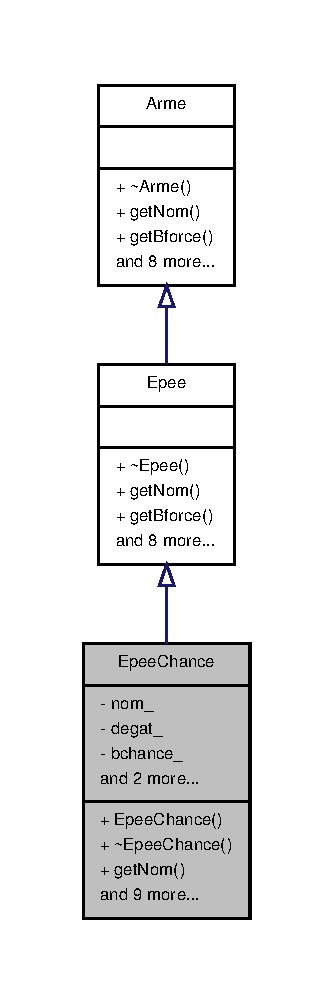
\includegraphics[width=160pt]{class_epee_chance__inherit__graph}
\end{center}
\end{figure}


Graphe de collaboration de Epee\-Chance\-:
\nopagebreak
\begin{figure}[H]
\begin{center}
\leavevmode
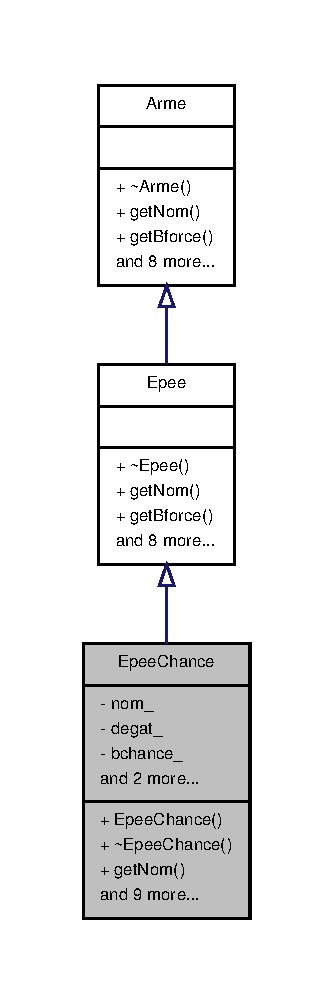
\includegraphics[width=160pt]{class_epee_chance__coll__graph}
\end{center}
\end{figure}
\subsection*{Fonctions membres publiques}
\begin{DoxyCompactItemize}
\item 
virtual std\-::string \hyperlink{class_arme_ab1b18cfa41fac19fccedf2165b9ff33c}{get\-Nom} ()
\begin{DoxyCompactList}\small\item\em Retourne le nom de l'arme. \end{DoxyCompactList}\item 
virtual int \hyperlink{class_arme_a3939e914a9ccc898de76db26bc8c24e7}{get\-Bforce} ()
\begin{DoxyCompactList}\small\item\em Retourne le bonus de force. \end{DoxyCompactList}\item 
virtual int \hyperlink{class_arme_a479453fea0d6789e34ccaf193b3098ce}{get\-Bvie} ()
\begin{DoxyCompactList}\small\item\em Retourne le bonus de vie. \end{DoxyCompactList}\item 
virtual int \hyperlink{class_arme_a6cb83d15008174152e424bebd0921069}{get\-Bchance} ()
\begin{DoxyCompactList}\small\item\em Retourne le bonus de chance. \end{DoxyCompactList}\item 
virtual int \hyperlink{class_arme_a06ced3532b0e60cc900674a94c0cf29b}{get\-Degat} ()
\begin{DoxyCompactList}\small\item\em Retourne les degats de l'arme. \end{DoxyCompactList}\end{DoxyCompactItemize}
\subsection*{Attributs protégés}
\begin{DoxyCompactItemize}
\item 
\hypertarget{class_arme_a347394a5ab5c3230259c1b7117f3e8d6}{std\-::string \hyperlink{class_arme_a347394a5ab5c3230259c1b7117f3e8d6}{nom\-\_\-}}\label{class_arme_a347394a5ab5c3230259c1b7117f3e8d6}

\begin{DoxyCompactList}\small\item\em Nom de l'arme. \end{DoxyCompactList}\item 
\hypertarget{class_arme_a15f99a8b95c2d6f5beb9f473df79e399}{int \hyperlink{class_arme_a15f99a8b95c2d6f5beb9f473df79e399}{degat\-\_\-}}\label{class_arme_a15f99a8b95c2d6f5beb9f473df79e399}

\begin{DoxyCompactList}\small\item\em Bonus de dégat. \end{DoxyCompactList}\item 
\hypertarget{class_arme_a688792d4393f9e690aa103a8e68c541c}{int \hyperlink{class_arme_a688792d4393f9e690aa103a8e68c541c}{bchance\-\_\-}}\label{class_arme_a688792d4393f9e690aa103a8e68c541c}

\begin{DoxyCompactList}\small\item\em Bonus de chance. \end{DoxyCompactList}\item 
\hypertarget{class_arme_a4606c075b38ef49f6ed2ed06d6185173}{int \hyperlink{class_arme_a4606c075b38ef49f6ed2ed06d6185173}{bvie\-\_\-}}\label{class_arme_a4606c075b38ef49f6ed2ed06d6185173}

\begin{DoxyCompactList}\small\item\em Bonus de vie. \end{DoxyCompactList}\item 
\hypertarget{class_arme_a779e9838aa9c50d948f58b593fc5954b}{int \hyperlink{class_arme_a779e9838aa9c50d948f58b593fc5954b}{bforce\-\_\-}}\label{class_arme_a779e9838aa9c50d948f58b593fc5954b}

\begin{DoxyCompactList}\small\item\em Bonus de force. \end{DoxyCompactList}\end{DoxyCompactItemize}


\subsection{Description détaillée}
\hyperlink{class_epee_chance}{Epee\-Chance} herite de \hyperlink{class_epee}{Epee}. 

\subsection{Documentation des fonctions membres}
\hypertarget{class_arme_a6cb83d15008174152e424bebd0921069}{\index{Epee\-Chance@{Epee\-Chance}!get\-Bchance@{get\-Bchance}}
\index{get\-Bchance@{get\-Bchance}!EpeeChance@{Epee\-Chance}}
\subsubsection[{get\-Bchance}]{\setlength{\rightskip}{0pt plus 5cm}int Arme\-::get\-Bchance (
\begin{DoxyParamCaption}
{}
\end{DoxyParamCaption}
)\hspace{0.3cm}{\ttfamily [virtual]}, {\ttfamily [inherited]}}}\label{class_arme_a6cb83d15008174152e424bebd0921069}


Retourne le bonus de chance. 

\begin{DoxyReturn}{Renvoie}
Bchance 
\end{DoxyReturn}


Réimplémentée dans \hyperlink{class_d_arme_ad50d376b08d62276b7cf50d2cd59d619}{D\-Arme}.

\hypertarget{class_arme_a3939e914a9ccc898de76db26bc8c24e7}{\index{Epee\-Chance@{Epee\-Chance}!get\-Bforce@{get\-Bforce}}
\index{get\-Bforce@{get\-Bforce}!EpeeChance@{Epee\-Chance}}
\subsubsection[{get\-Bforce}]{\setlength{\rightskip}{0pt plus 5cm}int Arme\-::get\-Bforce (
\begin{DoxyParamCaption}
{}
\end{DoxyParamCaption}
)\hspace{0.3cm}{\ttfamily [virtual]}, {\ttfamily [inherited]}}}\label{class_arme_a3939e914a9ccc898de76db26bc8c24e7}


Retourne le bonus de force. 

\begin{DoxyReturn}{Renvoie}
Bforce 
\end{DoxyReturn}


Réimplémentée dans \hyperlink{class_d_arme_a76075bcbe61b20bd0e21e2d06fe33ab7}{D\-Arme}.

\hypertarget{class_arme_a479453fea0d6789e34ccaf193b3098ce}{\index{Epee\-Chance@{Epee\-Chance}!get\-Bvie@{get\-Bvie}}
\index{get\-Bvie@{get\-Bvie}!EpeeChance@{Epee\-Chance}}
\subsubsection[{get\-Bvie}]{\setlength{\rightskip}{0pt plus 5cm}int Arme\-::get\-Bvie (
\begin{DoxyParamCaption}
{}
\end{DoxyParamCaption}
)\hspace{0.3cm}{\ttfamily [virtual]}, {\ttfamily [inherited]}}}\label{class_arme_a479453fea0d6789e34ccaf193b3098ce}


Retourne le bonus de vie. 

\begin{DoxyReturn}{Renvoie}
Bvie 
\end{DoxyReturn}


Réimplémentée dans \hyperlink{class_d_arme_a91b3a3100969a568a8408ba098668398}{D\-Arme}.

\hypertarget{class_arme_a06ced3532b0e60cc900674a94c0cf29b}{\index{Epee\-Chance@{Epee\-Chance}!get\-Degat@{get\-Degat}}
\index{get\-Degat@{get\-Degat}!EpeeChance@{Epee\-Chance}}
\subsubsection[{get\-Degat}]{\setlength{\rightskip}{0pt plus 5cm}int Arme\-::get\-Degat (
\begin{DoxyParamCaption}
{}
\end{DoxyParamCaption}
)\hspace{0.3cm}{\ttfamily [virtual]}, {\ttfamily [inherited]}}}\label{class_arme_a06ced3532b0e60cc900674a94c0cf29b}


Retourne les degats de l'arme. 

\begin{DoxyReturn}{Renvoie}
degats 
\end{DoxyReturn}


Réimplémentée dans \hyperlink{class_d_arme_a7396e865674067f4f21a28e6babc0fad}{D\-Arme}.

\hypertarget{class_arme_ab1b18cfa41fac19fccedf2165b9ff33c}{\index{Epee\-Chance@{Epee\-Chance}!get\-Nom@{get\-Nom}}
\index{get\-Nom@{get\-Nom}!EpeeChance@{Epee\-Chance}}
\subsubsection[{get\-Nom}]{\setlength{\rightskip}{0pt plus 5cm}std\-::string Arme\-::get\-Nom (
\begin{DoxyParamCaption}
{}
\end{DoxyParamCaption}
)\hspace{0.3cm}{\ttfamily [virtual]}, {\ttfamily [inherited]}}}\label{class_arme_ab1b18cfa41fac19fccedf2165b9ff33c}


Retourne le nom de l'arme. 

\begin{DoxyReturn}{Renvoie}
Nom 
\end{DoxyReturn}

\hypertarget{class_epee_force}{\section{Référence de la classe Epee\-Force}
\label{class_epee_force}\index{Epee\-Force@{Epee\-Force}}
}


\hyperlink{class_epee_force}{Epee\-Force} herite de \hyperlink{class_epee}{Epee}.  




Graphe d'héritage de Epee\-Force\-:
\nopagebreak
\begin{figure}[H]
\begin{center}
\leavevmode
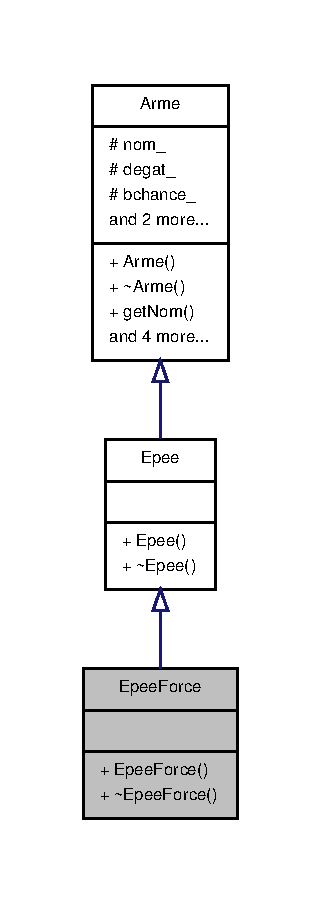
\includegraphics[width=154pt]{class_epee_force__inherit__graph}
\end{center}
\end{figure}


Graphe de collaboration de Epee\-Force\-:
\nopagebreak
\begin{figure}[H]
\begin{center}
\leavevmode
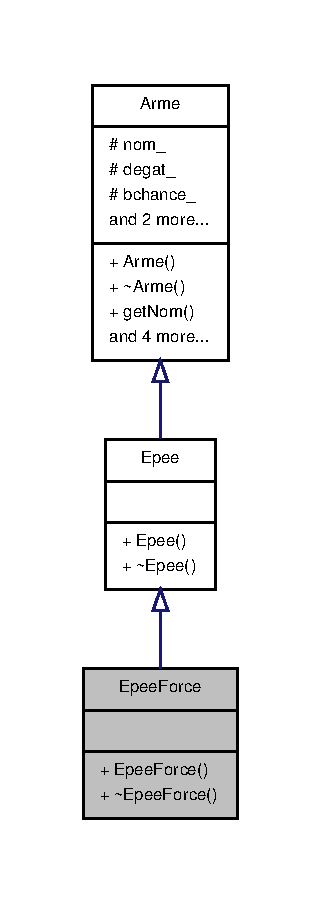
\includegraphics[width=154pt]{class_epee_force__coll__graph}
\end{center}
\end{figure}
\subsection*{Fonctions membres publiques}
\begin{DoxyCompactItemize}
\item 
virtual std\-::string \hyperlink{class_arme_ab1b18cfa41fac19fccedf2165b9ff33c}{get\-Nom} ()
\begin{DoxyCompactList}\small\item\em Retourne le nom de l'arme. \end{DoxyCompactList}\item 
virtual int \hyperlink{class_arme_a3939e914a9ccc898de76db26bc8c24e7}{get\-Bforce} ()
\begin{DoxyCompactList}\small\item\em Retourne le bonus de force. \end{DoxyCompactList}\item 
virtual int \hyperlink{class_arme_a479453fea0d6789e34ccaf193b3098ce}{get\-Bvie} ()
\begin{DoxyCompactList}\small\item\em Retourne le bonus de vie. \end{DoxyCompactList}\item 
virtual int \hyperlink{class_arme_a6cb83d15008174152e424bebd0921069}{get\-Bchance} ()
\begin{DoxyCompactList}\small\item\em Retourne le bonus de chance. \end{DoxyCompactList}\item 
virtual int \hyperlink{class_arme_a06ced3532b0e60cc900674a94c0cf29b}{get\-Degat} ()
\begin{DoxyCompactList}\small\item\em Retourne les degats de l'arme. \end{DoxyCompactList}\end{DoxyCompactItemize}
\subsection*{Attributs protégés}
\begin{DoxyCompactItemize}
\item 
\hypertarget{class_arme_a347394a5ab5c3230259c1b7117f3e8d6}{std\-::string \hyperlink{class_arme_a347394a5ab5c3230259c1b7117f3e8d6}{nom\-\_\-}}\label{class_arme_a347394a5ab5c3230259c1b7117f3e8d6}

\begin{DoxyCompactList}\small\item\em Nom de l'arme. \end{DoxyCompactList}\item 
\hypertarget{class_arme_a15f99a8b95c2d6f5beb9f473df79e399}{int \hyperlink{class_arme_a15f99a8b95c2d6f5beb9f473df79e399}{degat\-\_\-}}\label{class_arme_a15f99a8b95c2d6f5beb9f473df79e399}

\begin{DoxyCompactList}\small\item\em Bonus de dégat. \end{DoxyCompactList}\item 
\hypertarget{class_arme_a688792d4393f9e690aa103a8e68c541c}{int \hyperlink{class_arme_a688792d4393f9e690aa103a8e68c541c}{bchance\-\_\-}}\label{class_arme_a688792d4393f9e690aa103a8e68c541c}

\begin{DoxyCompactList}\small\item\em Bonus de chance. \end{DoxyCompactList}\item 
\hypertarget{class_arme_a4606c075b38ef49f6ed2ed06d6185173}{int \hyperlink{class_arme_a4606c075b38ef49f6ed2ed06d6185173}{bvie\-\_\-}}\label{class_arme_a4606c075b38ef49f6ed2ed06d6185173}

\begin{DoxyCompactList}\small\item\em Bonus de vie. \end{DoxyCompactList}\item 
\hypertarget{class_arme_a779e9838aa9c50d948f58b593fc5954b}{int \hyperlink{class_arme_a779e9838aa9c50d948f58b593fc5954b}{bforce\-\_\-}}\label{class_arme_a779e9838aa9c50d948f58b593fc5954b}

\begin{DoxyCompactList}\small\item\em Bonus de force. \end{DoxyCompactList}\end{DoxyCompactItemize}


\subsection{Description détaillée}
\hyperlink{class_epee_force}{Epee\-Force} herite de \hyperlink{class_epee}{Epee}. 

\subsection{Documentation des fonctions membres}
\hypertarget{class_arme_a6cb83d15008174152e424bebd0921069}{\index{Epee\-Force@{Epee\-Force}!get\-Bchance@{get\-Bchance}}
\index{get\-Bchance@{get\-Bchance}!EpeeForce@{Epee\-Force}}
\subsubsection[{get\-Bchance}]{\setlength{\rightskip}{0pt plus 5cm}int Arme\-::get\-Bchance (
\begin{DoxyParamCaption}
{}
\end{DoxyParamCaption}
)\hspace{0.3cm}{\ttfamily [virtual]}, {\ttfamily [inherited]}}}\label{class_arme_a6cb83d15008174152e424bebd0921069}


Retourne le bonus de chance. 

\begin{DoxyReturn}{Renvoie}
Bchance 
\end{DoxyReturn}


Réimplémentée dans \hyperlink{class_d_arme_ad50d376b08d62276b7cf50d2cd59d619}{D\-Arme}.

\hypertarget{class_arme_a3939e914a9ccc898de76db26bc8c24e7}{\index{Epee\-Force@{Epee\-Force}!get\-Bforce@{get\-Bforce}}
\index{get\-Bforce@{get\-Bforce}!EpeeForce@{Epee\-Force}}
\subsubsection[{get\-Bforce}]{\setlength{\rightskip}{0pt plus 5cm}int Arme\-::get\-Bforce (
\begin{DoxyParamCaption}
{}
\end{DoxyParamCaption}
)\hspace{0.3cm}{\ttfamily [virtual]}, {\ttfamily [inherited]}}}\label{class_arme_a3939e914a9ccc898de76db26bc8c24e7}


Retourne le bonus de force. 

\begin{DoxyReturn}{Renvoie}
Bforce 
\end{DoxyReturn}


Réimplémentée dans \hyperlink{class_d_arme_a76075bcbe61b20bd0e21e2d06fe33ab7}{D\-Arme}.

\hypertarget{class_arme_a479453fea0d6789e34ccaf193b3098ce}{\index{Epee\-Force@{Epee\-Force}!get\-Bvie@{get\-Bvie}}
\index{get\-Bvie@{get\-Bvie}!EpeeForce@{Epee\-Force}}
\subsubsection[{get\-Bvie}]{\setlength{\rightskip}{0pt plus 5cm}int Arme\-::get\-Bvie (
\begin{DoxyParamCaption}
{}
\end{DoxyParamCaption}
)\hspace{0.3cm}{\ttfamily [virtual]}, {\ttfamily [inherited]}}}\label{class_arme_a479453fea0d6789e34ccaf193b3098ce}


Retourne le bonus de vie. 

\begin{DoxyReturn}{Renvoie}
Bvie 
\end{DoxyReturn}


Réimplémentée dans \hyperlink{class_d_arme_a91b3a3100969a568a8408ba098668398}{D\-Arme}.

\hypertarget{class_arme_a06ced3532b0e60cc900674a94c0cf29b}{\index{Epee\-Force@{Epee\-Force}!get\-Degat@{get\-Degat}}
\index{get\-Degat@{get\-Degat}!EpeeForce@{Epee\-Force}}
\subsubsection[{get\-Degat}]{\setlength{\rightskip}{0pt plus 5cm}int Arme\-::get\-Degat (
\begin{DoxyParamCaption}
{}
\end{DoxyParamCaption}
)\hspace{0.3cm}{\ttfamily [virtual]}, {\ttfamily [inherited]}}}\label{class_arme_a06ced3532b0e60cc900674a94c0cf29b}


Retourne les degats de l'arme. 

\begin{DoxyReturn}{Renvoie}
degats 
\end{DoxyReturn}


Réimplémentée dans \hyperlink{class_d_arme_a7396e865674067f4f21a28e6babc0fad}{D\-Arme}.

\hypertarget{class_arme_ab1b18cfa41fac19fccedf2165b9ff33c}{\index{Epee\-Force@{Epee\-Force}!get\-Nom@{get\-Nom}}
\index{get\-Nom@{get\-Nom}!EpeeForce@{Epee\-Force}}
\subsubsection[{get\-Nom}]{\setlength{\rightskip}{0pt plus 5cm}std\-::string Arme\-::get\-Nom (
\begin{DoxyParamCaption}
{}
\end{DoxyParamCaption}
)\hspace{0.3cm}{\ttfamily [virtual]}, {\ttfamily [inherited]}}}\label{class_arme_ab1b18cfa41fac19fccedf2165b9ff33c}


Retourne le nom de l'arme. 

\begin{DoxyReturn}{Renvoie}
Nom 
\end{DoxyReturn}

\section{Référence de la classe Epee\-Vie}
\label{class_epee_vie}\index{Epee\-Vie@{Epee\-Vie}}


Graphe d'héritage de Epee\-Vie\-:\nopagebreak
\begin{figure}[H]
\begin{center}
\leavevmode
\includegraphics[width=144pt]{class_epee_vie__inherit__graph}
\end{center}
\end{figure}


Graphe de collaboration de Epee\-Vie\-:\nopagebreak
\begin{figure}[H]
\begin{center}
\leavevmode
\includegraphics[width=144pt]{class_epee_vie__coll__graph}
\end{center}
\end{figure}
\subsection*{Fonctions membres publiques}
\begin{DoxyCompactItemize}
\item 
{\bf Epee\-Vie} ()
\item 
{\bf $\sim$\-Epee\-Vie} ()
\item 
std\-::string {\bf get\-Nom} ()
\item 
int {\bf get\-Bforce} ()
\item 
int {\bf get\-Bvie} ()
\item 
int {\bf get\-Bchance} ()
\item 
int {\bf get\-Degat} ()
\item 
void {\bf set\-Bforce} (int bforce)
\item 
void {\bf set\-Bvie} (int bvie)
\item 
void {\bf set\-Bchance} (int bchance)
\item 
void {\bf set\-Degat} (int degat)
\item 
void {\bf set\-Nom} (std\-::string nom)
\end{DoxyCompactItemize}
\subsection*{Attributs privés}
\begin{DoxyCompactItemize}
\item 
std\-::string {\bf nom\-\_\-}
\item 
int {\bf degat\-\_\-}
\item 
int {\bf bchance\-\_\-}
\item 
int {\bf bvie\-\_\-}
\item 
int {\bf bforce\-\_\-}
\end{DoxyCompactItemize}


\subsection{Documentation des constructeurs et destructeur}
\index{Epee\-Vie@{Epee\-Vie}!Epee\-Vie@{Epee\-Vie}}
\index{Epee\-Vie@{Epee\-Vie}!EpeeVie@{Epee\-Vie}}
\subsubsection[{Epee\-Vie}]{\setlength{\rightskip}{0pt plus 5cm}Epee\-Vie\-::\-Epee\-Vie (
\begin{DoxyParamCaption}
{}
\end{DoxyParamCaption}
)}\label{class_epee_vie_a158348e32b3adbdc081b62a6faa612dc}
\index{Epee\-Vie@{Epee\-Vie}!$\sim$\-Epee\-Vie@{$\sim$\-Epee\-Vie}}
\index{$\sim$\-Epee\-Vie@{$\sim$\-Epee\-Vie}!EpeeVie@{Epee\-Vie}}
\subsubsection[{$\sim$\-Epee\-Vie}]{\setlength{\rightskip}{0pt plus 5cm}Epee\-Vie\-::$\sim$\-Epee\-Vie (
\begin{DoxyParamCaption}
{}
\end{DoxyParamCaption}
)}\label{class_epee_vie_a8ea7207b9cc1b86341ea18e629d48845}


\subsection{Documentation des fonctions membres}
\index{Epee\-Vie@{Epee\-Vie}!get\-Bchance@{get\-Bchance}}
\index{get\-Bchance@{get\-Bchance}!EpeeVie@{Epee\-Vie}}
\subsubsection[{get\-Bchance}]{\setlength{\rightskip}{0pt plus 5cm}int Epee\-Vie\-::get\-Bchance (
\begin{DoxyParamCaption}
{}
\end{DoxyParamCaption}
)\hspace{0.3cm}{\ttfamily [virtual]}}\label{class_epee_vie_af76e20e49e303804aa8ea2883228089b}


Implémente {\bf Epee} \doxyref{}{p.}{class_epee_ad1fb2f650193d85218f0f9742bac8e26}.

\index{Epee\-Vie@{Epee\-Vie}!get\-Bforce@{get\-Bforce}}
\index{get\-Bforce@{get\-Bforce}!EpeeVie@{Epee\-Vie}}
\subsubsection[{get\-Bforce}]{\setlength{\rightskip}{0pt plus 5cm}int Epee\-Vie\-::get\-Bforce (
\begin{DoxyParamCaption}
{}
\end{DoxyParamCaption}
)\hspace{0.3cm}{\ttfamily [virtual]}}\label{class_epee_vie_a848e8f74dfb7b4aa13b23cb1174964d7}


Implémente {\bf Epee} \doxyref{}{p.}{class_epee_a1e4ac064617efa372aa48e122da62da5}.

\index{Epee\-Vie@{Epee\-Vie}!get\-Bvie@{get\-Bvie}}
\index{get\-Bvie@{get\-Bvie}!EpeeVie@{Epee\-Vie}}
\subsubsection[{get\-Bvie}]{\setlength{\rightskip}{0pt plus 5cm}int Epee\-Vie\-::get\-Bvie (
\begin{DoxyParamCaption}
{}
\end{DoxyParamCaption}
)\hspace{0.3cm}{\ttfamily [virtual]}}\label{class_epee_vie_af3694dc84eff46350825f7e4955afa90}


Implémente {\bf Epee} \doxyref{}{p.}{class_epee_ae3e836b6821474eaa93653148404fb72}.

\index{Epee\-Vie@{Epee\-Vie}!get\-Degat@{get\-Degat}}
\index{get\-Degat@{get\-Degat}!EpeeVie@{Epee\-Vie}}
\subsubsection[{get\-Degat}]{\setlength{\rightskip}{0pt plus 5cm}int Epee\-Vie\-::get\-Degat (
\begin{DoxyParamCaption}
{}
\end{DoxyParamCaption}
)\hspace{0.3cm}{\ttfamily [virtual]}}\label{class_epee_vie_aede2704c0cb5f4339e6d14f0f4267d36}


Implémente {\bf Epee} \doxyref{}{p.}{class_epee_a389f6107671a22f69cca040d63aef647}.

\index{Epee\-Vie@{Epee\-Vie}!get\-Nom@{get\-Nom}}
\index{get\-Nom@{get\-Nom}!EpeeVie@{Epee\-Vie}}
\subsubsection[{get\-Nom}]{\setlength{\rightskip}{0pt plus 5cm}std\-::string Epee\-Vie\-::get\-Nom (
\begin{DoxyParamCaption}
{}
\end{DoxyParamCaption}
)\hspace{0.3cm}{\ttfamily [virtual]}}\label{class_epee_vie_a850643675b0b126aeedcf33d75fcd9e8}


Implémente {\bf Epee} \doxyref{}{p.}{class_epee_a3a006ae3e7e9f3275100a76f572dc085}.

\index{Epee\-Vie@{Epee\-Vie}!set\-Bchance@{set\-Bchance}}
\index{set\-Bchance@{set\-Bchance}!EpeeVie@{Epee\-Vie}}
\subsubsection[{set\-Bchance}]{\setlength{\rightskip}{0pt plus 5cm}void Epee\-Vie\-::set\-Bchance (
\begin{DoxyParamCaption}
\item[{int}]{bchance}
\end{DoxyParamCaption}
)\hspace{0.3cm}{\ttfamily [virtual]}}\label{class_epee_vie_abb56e1ae6ee02d815e56ad9ea68bd082}


Implémente {\bf Epee} \doxyref{}{p.}{class_epee_ac88031cb62f0c374ae0873ccd99d91bf}.

\index{Epee\-Vie@{Epee\-Vie}!set\-Bforce@{set\-Bforce}}
\index{set\-Bforce@{set\-Bforce}!EpeeVie@{Epee\-Vie}}
\subsubsection[{set\-Bforce}]{\setlength{\rightskip}{0pt plus 5cm}void Epee\-Vie\-::set\-Bforce (
\begin{DoxyParamCaption}
\item[{int}]{bforce}
\end{DoxyParamCaption}
)\hspace{0.3cm}{\ttfamily [virtual]}}\label{class_epee_vie_aaff428a4663555db0520e3528c8964d5}


Implémente {\bf Epee} \doxyref{}{p.}{class_epee_a98bc94805ee7d9d64a4e2f775bedb9d7}.

\index{Epee\-Vie@{Epee\-Vie}!set\-Bvie@{set\-Bvie}}
\index{set\-Bvie@{set\-Bvie}!EpeeVie@{Epee\-Vie}}
\subsubsection[{set\-Bvie}]{\setlength{\rightskip}{0pt plus 5cm}void Epee\-Vie\-::set\-Bvie (
\begin{DoxyParamCaption}
\item[{int}]{bvie}
\end{DoxyParamCaption}
)\hspace{0.3cm}{\ttfamily [virtual]}}\label{class_epee_vie_a0f8f49a705cc0b8be0417e2aba4bdf11}


Implémente {\bf Epee} \doxyref{}{p.}{class_epee_a643a5177f1f211c080c546430c1c4967}.

\index{Epee\-Vie@{Epee\-Vie}!set\-Degat@{set\-Degat}}
\index{set\-Degat@{set\-Degat}!EpeeVie@{Epee\-Vie}}
\subsubsection[{set\-Degat}]{\setlength{\rightskip}{0pt plus 5cm}void Epee\-Vie\-::set\-Degat (
\begin{DoxyParamCaption}
\item[{int}]{degat}
\end{DoxyParamCaption}
)\hspace{0.3cm}{\ttfamily [virtual]}}\label{class_epee_vie_a0a0ddd9571b2f9ea9c837b082d0bb680}


Implémente {\bf Epee} \doxyref{}{p.}{class_epee_a35ed08f9927b855b5b09643d00297dbc}.

\index{Epee\-Vie@{Epee\-Vie}!set\-Nom@{set\-Nom}}
\index{set\-Nom@{set\-Nom}!EpeeVie@{Epee\-Vie}}
\subsubsection[{set\-Nom}]{\setlength{\rightskip}{0pt plus 5cm}void Epee\-Vie\-::set\-Nom (
\begin{DoxyParamCaption}
\item[{std\-::string}]{nom}
\end{DoxyParamCaption}
)\hspace{0.3cm}{\ttfamily [virtual]}}\label{class_epee_vie_a32ca3accce018500c19a225e34eea7f8}


Implémente {\bf Epee} \doxyref{}{p.}{class_epee_a974abf77e22496b7d54f2357fbd664a2}.



\subsection{Documentation des données membres}
\index{Epee\-Vie@{Epee\-Vie}!bchance\-\_\-@{bchance\-\_\-}}
\index{bchance\-\_\-@{bchance\-\_\-}!EpeeVie@{Epee\-Vie}}
\subsubsection[{bchance\-\_\-}]{\setlength{\rightskip}{0pt plus 5cm}int Epee\-Vie\-::bchance\-\_\-\hspace{0.3cm}{\ttfamily [private]}}\label{class_epee_vie_a77a69912aa614ad962d2141d87cf6dce}
\index{Epee\-Vie@{Epee\-Vie}!bforce\-\_\-@{bforce\-\_\-}}
\index{bforce\-\_\-@{bforce\-\_\-}!EpeeVie@{Epee\-Vie}}
\subsubsection[{bforce\-\_\-}]{\setlength{\rightskip}{0pt plus 5cm}int Epee\-Vie\-::bforce\-\_\-\hspace{0.3cm}{\ttfamily [private]}}\label{class_epee_vie_af69e93134f9a3249d21965397f729c14}
\index{Epee\-Vie@{Epee\-Vie}!bvie\-\_\-@{bvie\-\_\-}}
\index{bvie\-\_\-@{bvie\-\_\-}!EpeeVie@{Epee\-Vie}}
\subsubsection[{bvie\-\_\-}]{\setlength{\rightskip}{0pt plus 5cm}int Epee\-Vie\-::bvie\-\_\-\hspace{0.3cm}{\ttfamily [private]}}\label{class_epee_vie_a9bcb222a3b45cebe97279ca4c1d01797}
\index{Epee\-Vie@{Epee\-Vie}!degat\-\_\-@{degat\-\_\-}}
\index{degat\-\_\-@{degat\-\_\-}!EpeeVie@{Epee\-Vie}}
\subsubsection[{degat\-\_\-}]{\setlength{\rightskip}{0pt plus 5cm}int Epee\-Vie\-::degat\-\_\-\hspace{0.3cm}{\ttfamily [private]}}\label{class_epee_vie_ae322e1c00d751c41b4f4b188aa62c18c}
\index{Epee\-Vie@{Epee\-Vie}!nom\-\_\-@{nom\-\_\-}}
\index{nom\-\_\-@{nom\-\_\-}!EpeeVie@{Epee\-Vie}}
\subsubsection[{nom\-\_\-}]{\setlength{\rightskip}{0pt plus 5cm}std\-::string Epee\-Vie\-::nom\-\_\-\hspace{0.3cm}{\ttfamily [private]}}\label{class_epee_vie_a4e61e0cab875ffde03bbc65692676247}


La documentation de cette classe a été générée à partir du fichier suivant \-:\begin{DoxyCompactItemize}
\item 
src/{\bf Epee\-Vie.\-hpp}\end{DoxyCompactItemize}

\hypertarget{class_equipement}{\section{Référence de la classe Equipement}
\label{class_equipement}\index{Equipement@{Equipement}}
}


Gestion des equipements.  




Graphe d'héritage de Equipement\-:
\nopagebreak
\begin{figure}[H]
\begin{center}
\leavevmode
\includegraphics[width=350pt]{class_equipement__inherit__graph}
\end{center}
\end{figure}


Graphe de collaboration de Equipement\-:
\nopagebreak
\begin{figure}[H]
\begin{center}
\leavevmode
\includegraphics[width=156pt]{class_equipement__coll__graph}
\end{center}
\end{figure}
\subsection*{Fonctions membres publiques}
\begin{DoxyCompactItemize}
\item 
virtual std\-::string \hyperlink{class_equipement_a0b0426a70bfce6e7c3efac605b75cd8e}{get\-Nom} ()
\begin{DoxyCompactList}\small\item\em Retourne le nom de l'equipement. \end{DoxyCompactList}\item 
virtual int \hyperlink{class_equipement_aabcf10fd762945fa4a37a9cf8321f463}{get\-Bforce} ()
\begin{DoxyCompactList}\small\item\em Retourne le bonus de force. \end{DoxyCompactList}\item 
virtual int \hyperlink{class_equipement_ad9fd7528c4f181970b7a0877f4145f89}{get\-Bvie} ()
\begin{DoxyCompactList}\small\item\em Retourne le bonus de vie. \end{DoxyCompactList}\item 
virtual int \hyperlink{class_equipement_a73485135eacdf30d5f49c9e34e5f4d0e}{get\-Bchance} ()
\begin{DoxyCompactList}\small\item\em Retourne le bonus de chance. \end{DoxyCompactList}\item 
virtual int \hyperlink{class_equipement_a8577d49fd00b8effa39388feccb29901}{get\-Armure} ()
\begin{DoxyCompactList}\small\item\em Retourne l'armure fournie par l'equipement. \end{DoxyCompactList}\item 
virtual int \hyperlink{class_equipement_a05b2c9d4cf22b6aefb6603fa4e322aa2}{type} ()=0
\begin{DoxyCompactList}\small\item\em Renvoie le type de l'equipement. \end{DoxyCompactList}\end{DoxyCompactItemize}
\subsection*{Attributs protégés}
\begin{DoxyCompactItemize}
\item 
\hypertarget{class_equipement_a930290aac01ecd40c7a646ab8f66d742}{std\-::string {\bfseries nom\-\_\-}}\label{class_equipement_a930290aac01ecd40c7a646ab8f66d742}

\item 
\hypertarget{class_equipement_a69339ce4f1f5fe7e6fcdeda5b74c14a4}{int {\bfseries armure\-\_\-}}\label{class_equipement_a69339ce4f1f5fe7e6fcdeda5b74c14a4}

\item 
\hypertarget{class_equipement_aa70effa6a8144fe1f4fe874af7139793}{int {\bfseries bchance\-\_\-}}\label{class_equipement_aa70effa6a8144fe1f4fe874af7139793}

\item 
\hypertarget{class_equipement_a73ac5bff40e3f6bf1d8e6f0e524e750f}{int {\bfseries bvie\-\_\-}}\label{class_equipement_a73ac5bff40e3f6bf1d8e6f0e524e750f}

\item 
\hypertarget{class_equipement_af87cf3f291386d5401be6994dd8fb8be}{int {\bfseries bforce\-\_\-}}\label{class_equipement_af87cf3f291386d5401be6994dd8fb8be}

\end{DoxyCompactItemize}


\subsection{Description détaillée}
Gestion des equipements. 

\subsection{Documentation des fonctions membres}
\hypertarget{class_equipement_a8577d49fd00b8effa39388feccb29901}{\index{Equipement@{Equipement}!get\-Armure@{get\-Armure}}
\index{get\-Armure@{get\-Armure}!Equipement@{Equipement}}
\subsubsection[{get\-Armure}]{\setlength{\rightskip}{0pt plus 5cm}int Equipement\-::get\-Armure (
\begin{DoxyParamCaption}
{}
\end{DoxyParamCaption}
)\hspace{0.3cm}{\ttfamily [virtual]}}}\label{class_equipement_a8577d49fd00b8effa39388feccb29901}


Retourne l'armure fournie par l'equipement. 

\begin{DoxyReturn}{Renvoie}
armure 
\end{DoxyReturn}


Réimplémentée dans \hyperlink{class_d_equip_a7b2c8227ae884c23ccc8f3a2e5702186}{D\-Equip}.

\hypertarget{class_equipement_a73485135eacdf30d5f49c9e34e5f4d0e}{\index{Equipement@{Equipement}!get\-Bchance@{get\-Bchance}}
\index{get\-Bchance@{get\-Bchance}!Equipement@{Equipement}}
\subsubsection[{get\-Bchance}]{\setlength{\rightskip}{0pt plus 5cm}int Equipement\-::get\-Bchance (
\begin{DoxyParamCaption}
{}
\end{DoxyParamCaption}
)\hspace{0.3cm}{\ttfamily [virtual]}}}\label{class_equipement_a73485135eacdf30d5f49c9e34e5f4d0e}


Retourne le bonus de chance. 

\begin{DoxyReturn}{Renvoie}
Bchance 
\end{DoxyReturn}


Réimplémentée dans \hyperlink{class_d_equip_a39407c92f0de87306a33f57fd22ce997}{D\-Equip}.

\hypertarget{class_equipement_aabcf10fd762945fa4a37a9cf8321f463}{\index{Equipement@{Equipement}!get\-Bforce@{get\-Bforce}}
\index{get\-Bforce@{get\-Bforce}!Equipement@{Equipement}}
\subsubsection[{get\-Bforce}]{\setlength{\rightskip}{0pt plus 5cm}int Equipement\-::get\-Bforce (
\begin{DoxyParamCaption}
{}
\end{DoxyParamCaption}
)\hspace{0.3cm}{\ttfamily [virtual]}}}\label{class_equipement_aabcf10fd762945fa4a37a9cf8321f463}


Retourne le bonus de force. 

\begin{DoxyReturn}{Renvoie}
Bforce 
\end{DoxyReturn}


Réimplémentée dans \hyperlink{class_d_equip_adb6645ce01c12a4cb3fe0b522ea6b25e}{D\-Equip}.

\hypertarget{class_equipement_ad9fd7528c4f181970b7a0877f4145f89}{\index{Equipement@{Equipement}!get\-Bvie@{get\-Bvie}}
\index{get\-Bvie@{get\-Bvie}!Equipement@{Equipement}}
\subsubsection[{get\-Bvie}]{\setlength{\rightskip}{0pt plus 5cm}int Equipement\-::get\-Bvie (
\begin{DoxyParamCaption}
{}
\end{DoxyParamCaption}
)\hspace{0.3cm}{\ttfamily [virtual]}}}\label{class_equipement_ad9fd7528c4f181970b7a0877f4145f89}


Retourne le bonus de vie. 

\begin{DoxyReturn}{Renvoie}
Bvie 
\end{DoxyReturn}


Réimplémentée dans \hyperlink{class_d_equip_a085ea4ac21c238d8c147ff4e6d74794f}{D\-Equip}.

\hypertarget{class_equipement_a0b0426a70bfce6e7c3efac605b75cd8e}{\index{Equipement@{Equipement}!get\-Nom@{get\-Nom}}
\index{get\-Nom@{get\-Nom}!Equipement@{Equipement}}
\subsubsection[{get\-Nom}]{\setlength{\rightskip}{0pt plus 5cm}std\-::string Equipement\-::get\-Nom (
\begin{DoxyParamCaption}
{}
\end{DoxyParamCaption}
)\hspace{0.3cm}{\ttfamily [virtual]}}}\label{class_equipement_a0b0426a70bfce6e7c3efac605b75cd8e}


Retourne le nom de l'equipement. 

\begin{DoxyReturn}{Renvoie}
Nom 
\end{DoxyReturn}
\hypertarget{class_equipement_a05b2c9d4cf22b6aefb6603fa4e322aa2}{\index{Equipement@{Equipement}!type@{type}}
\index{type@{type}!Equipement@{Equipement}}
\subsubsection[{type}]{\setlength{\rightskip}{0pt plus 5cm}virtual int Equipement\-::type (
\begin{DoxyParamCaption}
{}
\end{DoxyParamCaption}
)\hspace{0.3cm}{\ttfamily [pure virtual]}}}\label{class_equipement_a05b2c9d4cf22b6aefb6603fa4e322aa2}


Renvoie le type de l'equipement. 

\begin{DoxyReturn}{Renvoie}
int 
\end{DoxyReturn}


Implémenté dans \hyperlink{class_d_equip_a7c31f807517e5940e899780ac6d7a5c3}{D\-Equip}, \hyperlink{class_jambe_a2a996cd6338e990408ef3394e4f05789}{Jambe}, \hyperlink{class_torse_ae10a627f995808454342b4c853c5a162}{Torse}, et \hyperlink{class_casque_acb93c4c89d61c945d75ee3d47bede861}{Casque}.


\section{Référence de la classe Force\-Factory}
\label{class_force_factory}\index{Force\-Factory@{Force\-Factory}}


Factory concrete pour creer des objets de type Force.  




Graphe d'héritage de Force\-Factory\-:\nopagebreak
\begin{figure}[H]
\begin{center}
\leavevmode
\includegraphics[width=160pt]{class_force_factory__inherit__graph}
\end{center}
\end{figure}


Graphe de collaboration de Force\-Factory\-:\nopagebreak
\begin{figure}[H]
\begin{center}
\leavevmode
\includegraphics[width=160pt]{class_force_factory__coll__graph}
\end{center}
\end{figure}
\subsection*{Fonctions membres publiques}
\begin{DoxyCompactItemize}
\item 
{\bf Casque} $\ast$ {\bf Get\-Casque} ()
\begin{DoxyCompactList}\small\item\em Renvoie un pointeur vers un \doxyref{Casque}{p.}{class_casque} pour que la factory concrete connaisse l'objet a creer. \end{DoxyCompactList}\item 
{\bf Torse} $\ast$ {\bf Get\-Torse} ()
\begin{DoxyCompactList}\small\item\em Renvoie un pointeur vers un \doxyref{Torse}{p.}{class_torse} pour que la factory concrete connaisse l'objet a creer. \end{DoxyCompactList}\item 
{\bf Jambe} $\ast$ {\bf Get\-Jambe} ()
\begin{DoxyCompactList}\small\item\em Renvoie un pointeur vers \doxyref{Jambe}{p.}{class_jambe} pour que la factory concrete connaisse l'objet a creer. \end{DoxyCompactList}\item 
{\bf Epee} $\ast$ {\bf Get\-Epee} ()
\begin{DoxyCompactList}\small\item\em Renvoie un pointeur vers une \doxyref{Epee}{p.}{class_epee} pour que la factory concrete connaisse l'objet a creer. \end{DoxyCompactList}\item 
{\bf Dague} $\ast$ {\bf Get\-Dague} ()
\begin{DoxyCompactList}\small\item\em Renvoie un pointeur vers une \doxyref{Dague}{p.}{class_dague} pour que la factory concrete connaisse l'objet a creer. \end{DoxyCompactList}\item 
{\bf Hache} $\ast$ {\bf Get\-Hache} ()
\begin{DoxyCompactList}\small\item\em Renvoie un pointeur vers une \doxyref{Hache}{p.}{class_hache} pour que la factory concrete connaisse l'objet a creer. \end{DoxyCompactList}\end{DoxyCompactItemize}
\subsection*{Fonctions membres publiques statiques}
\begin{DoxyCompactItemize}
\item 
static {\bf Item\-Factory} $\ast$ {\bf Create\-Factory} ({\bf I\-T\-E\-M\-\_\-\-F\-A\-C\-T\-O\-R\-I\-E\-S} factory)
\begin{DoxyCompactList}\small\item\em Methode qui creer une factory concrete en fonction du type passe en parametre. \end{DoxyCompactList}\end{DoxyCompactItemize}


\subsection{Description détaillée}
Factory concrete pour creer des objets de type Force. 

\subsection{Documentation des fonctions membres}
\index{Force\-Factory@{Force\-Factory}!Create\-Factory@{Create\-Factory}}
\index{Create\-Factory@{Create\-Factory}!ForceFactory@{Force\-Factory}}
\subsubsection[{Create\-Factory}]{\setlength{\rightskip}{0pt plus 5cm}{\bf Item\-Factory} $\ast$ Item\-Factory\-::\-Create\-Factory (
\begin{DoxyParamCaption}
\item[{{\bf I\-T\-E\-M\-\_\-\-F\-A\-C\-T\-O\-R\-I\-E\-S}}]{factory}
\end{DoxyParamCaption}
)\hspace{0.3cm}{\ttfamily [static]}, {\ttfamily [inherited]}}\label{class_item_factory_ab10257decaf2cda946ec482a0dfdfe03}


Methode qui creer une factory concrete en fonction du type passe en parametre. 


\begin{DoxyParams}{Paramètres}
{\em I\-T\-E\-M\-\_\-\-F\-A\-C\-T\-O\-R\-I\-E\-S} & type de la factory \\
\hline
\end{DoxyParams}
\begin{DoxyReturn}{Renvoie}
Item\-Factory$\ast$ Pointeur vers une factory concrete 
\end{DoxyReturn}
\index{Force\-Factory@{Force\-Factory}!Get\-Casque@{Get\-Casque}}
\index{Get\-Casque@{Get\-Casque}!ForceFactory@{Force\-Factory}}
\subsubsection[{Get\-Casque}]{\setlength{\rightskip}{0pt plus 5cm}{\bf Casque} $\ast$ Force\-Factory\-::\-Get\-Casque (
\begin{DoxyParamCaption}
{}
\end{DoxyParamCaption}
)\hspace{0.3cm}{\ttfamily [virtual]}}\label{class_force_factory_af7a70ed4e427ff00a637613364e4e465}


Renvoie un pointeur vers un \doxyref{Casque}{p.}{class_casque} pour que la factory concrete connaisse l'objet a creer. 

\begin{DoxyReturn}{Renvoie}
Casque$\ast$ Pointeur vers \doxyref{Casque}{p.}{class_casque} 
\end{DoxyReturn}


Implémente {\bf Item\-Factory} \doxyref{}{p.}{class_item_factory_a89450cf0176a8da74cc5a9b8ef5aaae6}.

\index{Force\-Factory@{Force\-Factory}!Get\-Dague@{Get\-Dague}}
\index{Get\-Dague@{Get\-Dague}!ForceFactory@{Force\-Factory}}
\subsubsection[{Get\-Dague}]{\setlength{\rightskip}{0pt plus 5cm}{\bf Dague} $\ast$ Force\-Factory\-::\-Get\-Dague (
\begin{DoxyParamCaption}
{}
\end{DoxyParamCaption}
)\hspace{0.3cm}{\ttfamily [virtual]}}\label{class_force_factory_a868dd51ed72902455d44923b149ed01a}


Renvoie un pointeur vers une \doxyref{Dague}{p.}{class_dague} pour que la factory concrete connaisse l'objet a creer. 

\begin{DoxyReturn}{Renvoie}
\doxyref{Dague}{p.}{class_dague} $\ast$ Pointeur vers \doxyref{Dague}{p.}{class_dague} 
\end{DoxyReturn}


Implémente {\bf Item\-Factory} \doxyref{}{p.}{class_item_factory_a65ed7c9978011812487e6b12b4155fbd}.

\index{Force\-Factory@{Force\-Factory}!Get\-Epee@{Get\-Epee}}
\index{Get\-Epee@{Get\-Epee}!ForceFactory@{Force\-Factory}}
\subsubsection[{Get\-Epee}]{\setlength{\rightskip}{0pt plus 5cm}{\bf Epee} $\ast$ Force\-Factory\-::\-Get\-Epee (
\begin{DoxyParamCaption}
{}
\end{DoxyParamCaption}
)\hspace{0.3cm}{\ttfamily [virtual]}}\label{class_force_factory_a9b868013f6c513d1fb9cfe9dbf23e9c7}


Renvoie un pointeur vers une \doxyref{Epee}{p.}{class_epee} pour que la factory concrete connaisse l'objet a creer. 

\begin{DoxyReturn}{Renvoie}
\doxyref{Epee}{p.}{class_epee} $\ast$ Pointeur vers \doxyref{Epee}{p.}{class_epee} 
\end{DoxyReturn}


Implémente {\bf Item\-Factory} \doxyref{}{p.}{class_item_factory_a8a413e61bf23ad24a549382e4e4e396f}.

\index{Force\-Factory@{Force\-Factory}!Get\-Hache@{Get\-Hache}}
\index{Get\-Hache@{Get\-Hache}!ForceFactory@{Force\-Factory}}
\subsubsection[{Get\-Hache}]{\setlength{\rightskip}{0pt plus 5cm}{\bf Hache} $\ast$ Force\-Factory\-::\-Get\-Hache (
\begin{DoxyParamCaption}
{}
\end{DoxyParamCaption}
)\hspace{0.3cm}{\ttfamily [virtual]}}\label{class_force_factory_a38640ebadfea5fb945c27bc31097f56a}


Renvoie un pointeur vers une \doxyref{Hache}{p.}{class_hache} pour que la factory concrete connaisse l'objet a creer. 

\begin{DoxyReturn}{Renvoie}
\doxyref{Hache}{p.}{class_hache} $\ast$ Pointeur vers \doxyref{Hache}{p.}{class_hache} 
\end{DoxyReturn}


Implémente {\bf Item\-Factory} \doxyref{}{p.}{class_item_factory_afd402df71468d0a96ea12e92c80a185e}.

\index{Force\-Factory@{Force\-Factory}!Get\-Jambe@{Get\-Jambe}}
\index{Get\-Jambe@{Get\-Jambe}!ForceFactory@{Force\-Factory}}
\subsubsection[{Get\-Jambe}]{\setlength{\rightskip}{0pt plus 5cm}{\bf Jambe} $\ast$ Force\-Factory\-::\-Get\-Jambe (
\begin{DoxyParamCaption}
{}
\end{DoxyParamCaption}
)\hspace{0.3cm}{\ttfamily [virtual]}}\label{class_force_factory_a266b2440469141caf3cf1f7b7aadd3b4}


Renvoie un pointeur vers \doxyref{Jambe}{p.}{class_jambe} pour que la factory concrete connaisse l'objet a creer. 

\begin{DoxyReturn}{Renvoie}
\doxyref{Jambe}{p.}{class_jambe} $\ast$ Pointeur vers \doxyref{Jambe}{p.}{class_jambe} 
\end{DoxyReturn}


Implémente {\bf Item\-Factory} \doxyref{}{p.}{class_item_factory_a0a9cc8a72f93f260a61d393d8fb76012}.

\index{Force\-Factory@{Force\-Factory}!Get\-Torse@{Get\-Torse}}
\index{Get\-Torse@{Get\-Torse}!ForceFactory@{Force\-Factory}}
\subsubsection[{Get\-Torse}]{\setlength{\rightskip}{0pt plus 5cm}{\bf Torse} $\ast$ Force\-Factory\-::\-Get\-Torse (
\begin{DoxyParamCaption}
{}
\end{DoxyParamCaption}
)\hspace{0.3cm}{\ttfamily [virtual]}}\label{class_force_factory_adfe688df9ecf92a00558d8922635713e}


Renvoie un pointeur vers un \doxyref{Torse}{p.}{class_torse} pour que la factory concrete connaisse l'objet a creer. 

\begin{DoxyReturn}{Renvoie}
\doxyref{Torse}{p.}{class_torse} $\ast$ Pointeur vers \doxyref{Torse}{p.}{class_torse} 
\end{DoxyReturn}


Implémente {\bf Item\-Factory} \doxyref{}{p.}{class_item_factory_ad5f3eb7dffeed5577e05e859775af3dd}.



La documentation de cette classe a été générée à partir des fichiers suivants \-:\begin{DoxyCompactItemize}
\item 
src/{\bf Force\-Factory.\-hpp}\item 
src/{\bf Force\-Factory.\-cpp}\end{DoxyCompactItemize}

\section{Référence de la classe Game}
\label{class_game}\index{Game@{Game}}


Gère une partie manage un labyrinth avec un joueur.  




Graphe de collaboration de Game\-:\nopagebreak
\begin{figure}[H]
\begin{center}
\leavevmode
\includegraphics[width=350pt]{class_game__coll__graph}
\end{center}
\end{figure}
\subsection*{Fonctions membres publiques}
\begin{DoxyCompactItemize}
\item 
{\bf Game} (std\-::string name, int x={\bf L\-A\-B\-Y\-R\-I\-N\-T\-H\-\_\-\-T\-A\-I\-L\-L\-E\-\_\-\-X\-\_\-\-D\-E\-F\-A\-U\-L\-T}, int y={\bf L\-A\-B\-Y\-R\-I\-N\-T\-H\-\_\-\-T\-A\-I\-L\-L\-E\-\_\-\-Y\-\_\-\-D\-E\-F\-A\-U\-L\-T})
\begin{DoxyCompactList}\small\item\em constucteur \end{DoxyCompactList}\item 
void {\bf launch} ()
\begin{DoxyCompactList}\small\item\em Débute le déroulement d'une partie. \end{DoxyCompactList}\item 
void {\bf choose\-Room} ()
\begin{DoxyCompactList}\small\item\em Choisie une direction et execute l'action de la salle. \end{DoxyCompactList}\item 
void {\bf help} ()
\begin{DoxyCompactList}\small\item\em Affiche les commandes. \end{DoxyCompactList}\end{DoxyCompactItemize}
\subsection*{Attributs privés}
\begin{DoxyCompactItemize}
\item 
{\bf Labyrinth} {\bf m\-\_\-labyrinth}
\begin{DoxyCompactList}\small\item\em le labyrinthe \end{DoxyCompactList}\item 
{\bf Personnage} {\bf m\-\_\-perso}
\begin{DoxyCompactList}\small\item\em le personnage \end{DoxyCompactList}\end{DoxyCompactItemize}


\subsection{Description détaillée}
Gère une partie manage un labyrinth avec un joueur. 

\subsection{Documentation des constructeurs et destructeur}
\index{Game@{Game}!Game@{Game}}
\index{Game@{Game}!Game@{Game}}
\subsubsection[{Game}]{\setlength{\rightskip}{0pt plus 5cm}Game\-::\-Game (
\begin{DoxyParamCaption}
\item[{std\-::string}]{name, }
\item[{int}]{x = {\ttfamily {\bf L\-A\-B\-Y\-R\-I\-N\-T\-H\-\_\-\-T\-A\-I\-L\-L\-E\-\_\-\-X\-\_\-\-D\-E\-F\-A\-U\-L\-T}}, }
\item[{int}]{y = {\ttfamily {\bf L\-A\-B\-Y\-R\-I\-N\-T\-H\-\_\-\-T\-A\-I\-L\-L\-E\-\_\-\-Y\-\_\-\-D\-E\-F\-A\-U\-L\-T}}}
\end{DoxyParamCaption}
)}\label{class_game_af7c8b29a2938f3881bfd598e4e156d3d}


constucteur 


\begin{DoxyParams}{Paramètres}
{\em name} & nom du personnage \\
\hline
{\em x} & lageur \\
\hline
{\em y} & hauteur \\
\hline
\end{DoxyParams}


\subsection{Documentation des fonctions membres}
\index{Game@{Game}!choose\-Room@{choose\-Room}}
\index{choose\-Room@{choose\-Room}!Game@{Game}}
\subsubsection[{choose\-Room}]{\setlength{\rightskip}{0pt plus 5cm}void Game\-::choose\-Room (
\begin{DoxyParamCaption}
{}
\end{DoxyParamCaption}
)}\label{class_game_a70b3d987f25dd5e1aeb6ab18cfedc387}


Choisie une direction et execute l'action de la salle. 

\index{Game@{Game}!help@{help}}
\index{help@{help}!Game@{Game}}
\subsubsection[{help}]{\setlength{\rightskip}{0pt plus 5cm}void Game\-::help (
\begin{DoxyParamCaption}
{}
\end{DoxyParamCaption}
)}\label{class_game_ae650b8abcc603580654b9aa375dc260a}


Affiche les commandes. 

\index{Game@{Game}!launch@{launch}}
\index{launch@{launch}!Game@{Game}}
\subsubsection[{launch}]{\setlength{\rightskip}{0pt plus 5cm}void Game\-::launch (
\begin{DoxyParamCaption}
{}
\end{DoxyParamCaption}
)}\label{class_game_a35c46e76cde7773850820233754e0bc0}


Débute le déroulement d'une partie. 



\subsection{Documentation des données membres}
\index{Game@{Game}!m\-\_\-labyrinth@{m\-\_\-labyrinth}}
\index{m\-\_\-labyrinth@{m\-\_\-labyrinth}!Game@{Game}}
\subsubsection[{m\-\_\-labyrinth}]{\setlength{\rightskip}{0pt plus 5cm}{\bf Labyrinth} Game\-::m\-\_\-labyrinth\hspace{0.3cm}{\ttfamily [private]}}\label{class_game_ae240b11d8e568e768097735d85794d32}


le labyrinthe 

\index{Game@{Game}!m\-\_\-perso@{m\-\_\-perso}}
\index{m\-\_\-perso@{m\-\_\-perso}!Game@{Game}}
\subsubsection[{m\-\_\-perso}]{\setlength{\rightskip}{0pt plus 5cm}{\bf Personnage} Game\-::m\-\_\-perso\hspace{0.3cm}{\ttfamily [private]}}\label{class_game_aa61c11c5da4f4b2e977c230d8db13578}


le personnage 



La documentation de cette classe a été générée à partir des fichiers suivants \-:\begin{DoxyCompactItemize}
\item 
src/{\bf Game.\-hpp}\item 
src/{\bf Game.\-cpp}\end{DoxyCompactItemize}

\hypertarget{class_hache}{\section{Référence de la classe Hache}
\label{class_hache}\index{Hache@{Hache}}
}


\hyperlink{class_hache}{Hache} herite de \hyperlink{class_arme}{Arme}.  




Graphe d'héritage de Hache\-:
\nopagebreak
\begin{figure}[H]
\begin{center}
\leavevmode
\includegraphics[width=346pt]{class_hache__inherit__graph}
\end{center}
\end{figure}


Graphe de collaboration de Hache\-:
\nopagebreak
\begin{figure}[H]
\begin{center}
\leavevmode
\includegraphics[width=144pt]{class_hache__coll__graph}
\end{center}
\end{figure}
\subsection*{Fonctions membres publiques}
\begin{DoxyCompactItemize}
\item 
virtual std\-::string \hyperlink{class_arme_ab1b18cfa41fac19fccedf2165b9ff33c}{get\-Nom} ()
\begin{DoxyCompactList}\small\item\em Retourne le nom de l'arme. \end{DoxyCompactList}\item 
virtual int \hyperlink{class_arme_a3939e914a9ccc898de76db26bc8c24e7}{get\-Bforce} ()
\begin{DoxyCompactList}\small\item\em Retourne le bonus de force. \end{DoxyCompactList}\item 
virtual int \hyperlink{class_arme_a479453fea0d6789e34ccaf193b3098ce}{get\-Bvie} ()
\begin{DoxyCompactList}\small\item\em Retourne le bonus de vie. \end{DoxyCompactList}\item 
virtual int \hyperlink{class_arme_a6cb83d15008174152e424bebd0921069}{get\-Bchance} ()
\begin{DoxyCompactList}\small\item\em Retourne le bonus de chance. \end{DoxyCompactList}\item 
virtual int \hyperlink{class_arme_a06ced3532b0e60cc900674a94c0cf29b}{get\-Degat} ()
\begin{DoxyCompactList}\small\item\em Retourne les degats de l'arme. \end{DoxyCompactList}\end{DoxyCompactItemize}
\subsection*{Attributs protégés}
\begin{DoxyCompactItemize}
\item 
\hypertarget{class_arme_a347394a5ab5c3230259c1b7117f3e8d6}{std\-::string \hyperlink{class_arme_a347394a5ab5c3230259c1b7117f3e8d6}{nom\-\_\-}}\label{class_arme_a347394a5ab5c3230259c1b7117f3e8d6}

\begin{DoxyCompactList}\small\item\em Nom de l'arme. \end{DoxyCompactList}\item 
\hypertarget{class_arme_a15f99a8b95c2d6f5beb9f473df79e399}{int \hyperlink{class_arme_a15f99a8b95c2d6f5beb9f473df79e399}{degat\-\_\-}}\label{class_arme_a15f99a8b95c2d6f5beb9f473df79e399}

\begin{DoxyCompactList}\small\item\em Bonus de dégat. \end{DoxyCompactList}\item 
\hypertarget{class_arme_a688792d4393f9e690aa103a8e68c541c}{int \hyperlink{class_arme_a688792d4393f9e690aa103a8e68c541c}{bchance\-\_\-}}\label{class_arme_a688792d4393f9e690aa103a8e68c541c}

\begin{DoxyCompactList}\small\item\em Bonus de chance. \end{DoxyCompactList}\item 
\hypertarget{class_arme_a4606c075b38ef49f6ed2ed06d6185173}{int \hyperlink{class_arme_a4606c075b38ef49f6ed2ed06d6185173}{bvie\-\_\-}}\label{class_arme_a4606c075b38ef49f6ed2ed06d6185173}

\begin{DoxyCompactList}\small\item\em Bonus de vie. \end{DoxyCompactList}\item 
\hypertarget{class_arme_a779e9838aa9c50d948f58b593fc5954b}{int \hyperlink{class_arme_a779e9838aa9c50d948f58b593fc5954b}{bforce\-\_\-}}\label{class_arme_a779e9838aa9c50d948f58b593fc5954b}

\begin{DoxyCompactList}\small\item\em Bonus de force. \end{DoxyCompactList}\end{DoxyCompactItemize}


\subsection{Description détaillée}
\hyperlink{class_hache}{Hache} herite de \hyperlink{class_arme}{Arme}. 

\subsection{Documentation des fonctions membres}
\hypertarget{class_arme_a6cb83d15008174152e424bebd0921069}{\index{Hache@{Hache}!get\-Bchance@{get\-Bchance}}
\index{get\-Bchance@{get\-Bchance}!Hache@{Hache}}
\subsubsection[{get\-Bchance}]{\setlength{\rightskip}{0pt plus 5cm}int Arme\-::get\-Bchance (
\begin{DoxyParamCaption}
{}
\end{DoxyParamCaption}
)\hspace{0.3cm}{\ttfamily [virtual]}, {\ttfamily [inherited]}}}\label{class_arme_a6cb83d15008174152e424bebd0921069}


Retourne le bonus de chance. 

\begin{DoxyReturn}{Renvoie}
Bchance 
\end{DoxyReturn}


Réimplémentée dans \hyperlink{class_d_arme_ad50d376b08d62276b7cf50d2cd59d619}{D\-Arme}.

\hypertarget{class_arme_a3939e914a9ccc898de76db26bc8c24e7}{\index{Hache@{Hache}!get\-Bforce@{get\-Bforce}}
\index{get\-Bforce@{get\-Bforce}!Hache@{Hache}}
\subsubsection[{get\-Bforce}]{\setlength{\rightskip}{0pt plus 5cm}int Arme\-::get\-Bforce (
\begin{DoxyParamCaption}
{}
\end{DoxyParamCaption}
)\hspace{0.3cm}{\ttfamily [virtual]}, {\ttfamily [inherited]}}}\label{class_arme_a3939e914a9ccc898de76db26bc8c24e7}


Retourne le bonus de force. 

\begin{DoxyReturn}{Renvoie}
Bforce 
\end{DoxyReturn}


Réimplémentée dans \hyperlink{class_d_arme_a76075bcbe61b20bd0e21e2d06fe33ab7}{D\-Arme}.

\hypertarget{class_arme_a479453fea0d6789e34ccaf193b3098ce}{\index{Hache@{Hache}!get\-Bvie@{get\-Bvie}}
\index{get\-Bvie@{get\-Bvie}!Hache@{Hache}}
\subsubsection[{get\-Bvie}]{\setlength{\rightskip}{0pt plus 5cm}int Arme\-::get\-Bvie (
\begin{DoxyParamCaption}
{}
\end{DoxyParamCaption}
)\hspace{0.3cm}{\ttfamily [virtual]}, {\ttfamily [inherited]}}}\label{class_arme_a479453fea0d6789e34ccaf193b3098ce}


Retourne le bonus de vie. 

\begin{DoxyReturn}{Renvoie}
Bvie 
\end{DoxyReturn}


Réimplémentée dans \hyperlink{class_d_arme_a91b3a3100969a568a8408ba098668398}{D\-Arme}.

\hypertarget{class_arme_a06ced3532b0e60cc900674a94c0cf29b}{\index{Hache@{Hache}!get\-Degat@{get\-Degat}}
\index{get\-Degat@{get\-Degat}!Hache@{Hache}}
\subsubsection[{get\-Degat}]{\setlength{\rightskip}{0pt plus 5cm}int Arme\-::get\-Degat (
\begin{DoxyParamCaption}
{}
\end{DoxyParamCaption}
)\hspace{0.3cm}{\ttfamily [virtual]}, {\ttfamily [inherited]}}}\label{class_arme_a06ced3532b0e60cc900674a94c0cf29b}


Retourne les degats de l'arme. 

\begin{DoxyReturn}{Renvoie}
degats 
\end{DoxyReturn}


Réimplémentée dans \hyperlink{class_d_arme_a7396e865674067f4f21a28e6babc0fad}{D\-Arme}.

\hypertarget{class_arme_ab1b18cfa41fac19fccedf2165b9ff33c}{\index{Hache@{Hache}!get\-Nom@{get\-Nom}}
\index{get\-Nom@{get\-Nom}!Hache@{Hache}}
\subsubsection[{get\-Nom}]{\setlength{\rightskip}{0pt plus 5cm}std\-::string Arme\-::get\-Nom (
\begin{DoxyParamCaption}
{}
\end{DoxyParamCaption}
)\hspace{0.3cm}{\ttfamily [virtual]}, {\ttfamily [inherited]}}}\label{class_arme_ab1b18cfa41fac19fccedf2165b9ff33c}


Retourne le nom de l'arme. 

\begin{DoxyReturn}{Renvoie}
Nom 
\end{DoxyReturn}

\section{Référence de la classe Hache\-Chance}
\label{class_hache_chance}\index{Hache\-Chance@{Hache\-Chance}}


\doxyref{Hache\-Chance}{p.}{class_hache_chance} herite de \doxyref{Hache}{p.}{class_hache}.  




Graphe d'héritage de Hache\-Chance\-:\nopagebreak
\begin{figure}[H]
\begin{center}
\leavevmode
\includegraphics[width=164pt]{class_hache_chance__inherit__graph}
\end{center}
\end{figure}


Graphe de collaboration de Hache\-Chance\-:\nopagebreak
\begin{figure}[H]
\begin{center}
\leavevmode
\includegraphics[width=164pt]{class_hache_chance__coll__graph}
\end{center}
\end{figure}
\subsection*{Fonctions membres publiques}
\begin{DoxyCompactItemize}
\item 
{\bf Hache\-Chance} ()
\item 
{\bf $\sim$\-Hache\-Chance} ()
\item 
virtual std\-::string {\bf get\-Nom} ()
\begin{DoxyCompactList}\small\item\em Retourne le nom de l'arme. \end{DoxyCompactList}\item 
virtual int {\bf get\-Bforce} ()
\begin{DoxyCompactList}\small\item\em Retourne le bonus de force. \end{DoxyCompactList}\item 
virtual int {\bf get\-Bvie} ()
\begin{DoxyCompactList}\small\item\em Retourne le bonus de vie. \end{DoxyCompactList}\item 
virtual int {\bf get\-Bchance} ()
\begin{DoxyCompactList}\small\item\em Retourne le bonus de chance. \end{DoxyCompactList}\item 
virtual int {\bf get\-Degat} ()
\begin{DoxyCompactList}\small\item\em Retourne les degats de l'arme. \end{DoxyCompactList}\end{DoxyCompactItemize}
\subsection*{Attributs protégés}
\begin{DoxyCompactItemize}
\item 
std\-::string {\bf nom\-\_\-}
\begin{DoxyCompactList}\small\item\em Nom de l'arme. \end{DoxyCompactList}\item 
int {\bf degat\-\_\-}
\begin{DoxyCompactList}\small\item\em Bonus de dégat. \end{DoxyCompactList}\item 
int {\bf bchance\-\_\-}
\begin{DoxyCompactList}\small\item\em Bonus de chance. \end{DoxyCompactList}\item 
int {\bf bvie\-\_\-}
\begin{DoxyCompactList}\small\item\em Bonus de vie. \end{DoxyCompactList}\item 
int {\bf bforce\-\_\-}
\begin{DoxyCompactList}\small\item\em Bonus de force. \end{DoxyCompactList}\end{DoxyCompactItemize}


\subsection{Description détaillée}
\doxyref{Hache\-Chance}{p.}{class_hache_chance} herite de \doxyref{Hache}{p.}{class_hache}. 

\subsection{Documentation des constructeurs et destructeur}
\index{Hache\-Chance@{Hache\-Chance}!Hache\-Chance@{Hache\-Chance}}
\index{Hache\-Chance@{Hache\-Chance}!HacheChance@{Hache\-Chance}}
\subsubsection[{Hache\-Chance}]{\setlength{\rightskip}{0pt plus 5cm}Hache\-Chance\-::\-Hache\-Chance (
\begin{DoxyParamCaption}
{}
\end{DoxyParamCaption}
)}\label{class_hache_chance_aa849708389e41bac8953a403d07ce890}
\index{Hache\-Chance@{Hache\-Chance}!$\sim$\-Hache\-Chance@{$\sim$\-Hache\-Chance}}
\index{$\sim$\-Hache\-Chance@{$\sim$\-Hache\-Chance}!HacheChance@{Hache\-Chance}}
\subsubsection[{$\sim$\-Hache\-Chance}]{\setlength{\rightskip}{0pt plus 5cm}Hache\-Chance\-::$\sim$\-Hache\-Chance (
\begin{DoxyParamCaption}
{}
\end{DoxyParamCaption}
)}\label{class_hache_chance_aee4120dbef8f9c0984703b041603676e}


\subsection{Documentation des fonctions membres}
\index{Hache\-Chance@{Hache\-Chance}!get\-Bchance@{get\-Bchance}}
\index{get\-Bchance@{get\-Bchance}!HacheChance@{Hache\-Chance}}
\subsubsection[{get\-Bchance}]{\setlength{\rightskip}{0pt plus 5cm}int Arme\-::get\-Bchance (
\begin{DoxyParamCaption}
{}
\end{DoxyParamCaption}
)\hspace{0.3cm}{\ttfamily [virtual]}, {\ttfamily [inherited]}}\label{class_arme_a6cb83d15008174152e424bebd0921069}


Retourne le bonus de chance. 

\begin{DoxyReturn}{Renvoie}
Bchance 
\end{DoxyReturn}


Réimplémentée dans {\bf D\-Arme} \doxyref{}{p.}{class_d_arme_ad50d376b08d62276b7cf50d2cd59d619}.

\index{Hache\-Chance@{Hache\-Chance}!get\-Bforce@{get\-Bforce}}
\index{get\-Bforce@{get\-Bforce}!HacheChance@{Hache\-Chance}}
\subsubsection[{get\-Bforce}]{\setlength{\rightskip}{0pt plus 5cm}int Arme\-::get\-Bforce (
\begin{DoxyParamCaption}
{}
\end{DoxyParamCaption}
)\hspace{0.3cm}{\ttfamily [virtual]}, {\ttfamily [inherited]}}\label{class_arme_a3939e914a9ccc898de76db26bc8c24e7}


Retourne le bonus de force. 

\begin{DoxyReturn}{Renvoie}
Bforce 
\end{DoxyReturn}


Réimplémentée dans {\bf D\-Arme} \doxyref{}{p.}{class_d_arme_a76075bcbe61b20bd0e21e2d06fe33ab7}.

\index{Hache\-Chance@{Hache\-Chance}!get\-Bvie@{get\-Bvie}}
\index{get\-Bvie@{get\-Bvie}!HacheChance@{Hache\-Chance}}
\subsubsection[{get\-Bvie}]{\setlength{\rightskip}{0pt plus 5cm}int Arme\-::get\-Bvie (
\begin{DoxyParamCaption}
{}
\end{DoxyParamCaption}
)\hspace{0.3cm}{\ttfamily [virtual]}, {\ttfamily [inherited]}}\label{class_arme_a479453fea0d6789e34ccaf193b3098ce}


Retourne le bonus de vie. 

\begin{DoxyReturn}{Renvoie}
Bvie 
\end{DoxyReturn}


Réimplémentée dans {\bf D\-Arme} \doxyref{}{p.}{class_d_arme_a91b3a3100969a568a8408ba098668398}.

\index{Hache\-Chance@{Hache\-Chance}!get\-Degat@{get\-Degat}}
\index{get\-Degat@{get\-Degat}!HacheChance@{Hache\-Chance}}
\subsubsection[{get\-Degat}]{\setlength{\rightskip}{0pt plus 5cm}int Arme\-::get\-Degat (
\begin{DoxyParamCaption}
{}
\end{DoxyParamCaption}
)\hspace{0.3cm}{\ttfamily [virtual]}, {\ttfamily [inherited]}}\label{class_arme_a06ced3532b0e60cc900674a94c0cf29b}


Retourne les degats de l'arme. 

\begin{DoxyReturn}{Renvoie}
degats 
\end{DoxyReturn}


Réimplémentée dans {\bf D\-Arme} \doxyref{}{p.}{class_d_arme_a7396e865674067f4f21a28e6babc0fad}.

\index{Hache\-Chance@{Hache\-Chance}!get\-Nom@{get\-Nom}}
\index{get\-Nom@{get\-Nom}!HacheChance@{Hache\-Chance}}
\subsubsection[{get\-Nom}]{\setlength{\rightskip}{0pt plus 5cm}std\-::string Arme\-::get\-Nom (
\begin{DoxyParamCaption}
{}
\end{DoxyParamCaption}
)\hspace{0.3cm}{\ttfamily [virtual]}, {\ttfamily [inherited]}}\label{class_arme_ab1b18cfa41fac19fccedf2165b9ff33c}


Retourne le nom de l'arme. 

\begin{DoxyReturn}{Renvoie}
Nom 
\end{DoxyReturn}


\subsection{Documentation des données membres}
\index{Hache\-Chance@{Hache\-Chance}!bchance\-\_\-@{bchance\-\_\-}}
\index{bchance\-\_\-@{bchance\-\_\-}!HacheChance@{Hache\-Chance}}
\subsubsection[{bchance\-\_\-}]{\setlength{\rightskip}{0pt plus 5cm}int Arme\-::bchance\-\_\-\hspace{0.3cm}{\ttfamily [protected]}, {\ttfamily [inherited]}}\label{class_arme_a688792d4393f9e690aa103a8e68c541c}


Bonus de chance. 

\index{Hache\-Chance@{Hache\-Chance}!bforce\-\_\-@{bforce\-\_\-}}
\index{bforce\-\_\-@{bforce\-\_\-}!HacheChance@{Hache\-Chance}}
\subsubsection[{bforce\-\_\-}]{\setlength{\rightskip}{0pt plus 5cm}int Arme\-::bforce\-\_\-\hspace{0.3cm}{\ttfamily [protected]}, {\ttfamily [inherited]}}\label{class_arme_a779e9838aa9c50d948f58b593fc5954b}


Bonus de force. 

\index{Hache\-Chance@{Hache\-Chance}!bvie\-\_\-@{bvie\-\_\-}}
\index{bvie\-\_\-@{bvie\-\_\-}!HacheChance@{Hache\-Chance}}
\subsubsection[{bvie\-\_\-}]{\setlength{\rightskip}{0pt plus 5cm}int Arme\-::bvie\-\_\-\hspace{0.3cm}{\ttfamily [protected]}, {\ttfamily [inherited]}}\label{class_arme_a4606c075b38ef49f6ed2ed06d6185173}


Bonus de vie. 

\index{Hache\-Chance@{Hache\-Chance}!degat\-\_\-@{degat\-\_\-}}
\index{degat\-\_\-@{degat\-\_\-}!HacheChance@{Hache\-Chance}}
\subsubsection[{degat\-\_\-}]{\setlength{\rightskip}{0pt plus 5cm}int Arme\-::degat\-\_\-\hspace{0.3cm}{\ttfamily [protected]}, {\ttfamily [inherited]}}\label{class_arme_a15f99a8b95c2d6f5beb9f473df79e399}


Bonus de dégat. 

\index{Hache\-Chance@{Hache\-Chance}!nom\-\_\-@{nom\-\_\-}}
\index{nom\-\_\-@{nom\-\_\-}!HacheChance@{Hache\-Chance}}
\subsubsection[{nom\-\_\-}]{\setlength{\rightskip}{0pt plus 5cm}std\-::string Arme\-::nom\-\_\-\hspace{0.3cm}{\ttfamily [protected]}, {\ttfamily [inherited]}}\label{class_arme_a347394a5ab5c3230259c1b7117f3e8d6}


Nom de l'arme. 



La documentation de cette classe a été générée à partir des fichiers suivants \-:\begin{DoxyCompactItemize}
\item 
src/{\bf Hache\-Chance.\-hpp}\item 
src/{\bf Hache\-Chance.\-cpp}\end{DoxyCompactItemize}

\section{Référence de la classe Hache\-Force}
\label{class_hache_force}\index{Hache\-Force@{Hache\-Force}}


\doxyref{Hache\-Force}{p.}{class_hache_force} herite de \doxyref{Hache}{p.}{class_hache}.  




Graphe d'héritage de Hache\-Force\-:\nopagebreak
\begin{figure}[H]
\begin{center}
\leavevmode
\includegraphics[width=158pt]{class_hache_force__inherit__graph}
\end{center}
\end{figure}


Graphe de collaboration de Hache\-Force\-:\nopagebreak
\begin{figure}[H]
\begin{center}
\leavevmode
\includegraphics[width=158pt]{class_hache_force__coll__graph}
\end{center}
\end{figure}
\subsection*{Fonctions membres publiques}
\begin{DoxyCompactItemize}
\item 
{\bf Hache\-Force} ()
\item 
{\bf $\sim$\-Hache\-Force} ()
\item 
virtual std\-::string {\bf get\-Nom} ()
\begin{DoxyCompactList}\small\item\em Retourne le nom de l'arme. \end{DoxyCompactList}\item 
virtual int {\bf get\-Bforce} ()
\begin{DoxyCompactList}\small\item\em Retourne le bonus de force. \end{DoxyCompactList}\item 
virtual int {\bf get\-Bvie} ()
\begin{DoxyCompactList}\small\item\em Retourne le bonus de vie. \end{DoxyCompactList}\item 
virtual int {\bf get\-Bchance} ()
\begin{DoxyCompactList}\small\item\em Retourne le bonus de chance. \end{DoxyCompactList}\item 
virtual int {\bf get\-Degat} ()
\begin{DoxyCompactList}\small\item\em Retourne les degats de l'arme. \end{DoxyCompactList}\end{DoxyCompactItemize}
\subsection*{Attributs protégés}
\begin{DoxyCompactItemize}
\item 
std\-::string {\bf nom\-\_\-}
\begin{DoxyCompactList}\small\item\em Nom de l'arme. \end{DoxyCompactList}\item 
int {\bf degat\-\_\-}
\begin{DoxyCompactList}\small\item\em Bonus de dégat. \end{DoxyCompactList}\item 
int {\bf bchance\-\_\-}
\begin{DoxyCompactList}\small\item\em Bonus de chance. \end{DoxyCompactList}\item 
int {\bf bvie\-\_\-}
\begin{DoxyCompactList}\small\item\em Bonus de vie. \end{DoxyCompactList}\item 
int {\bf bforce\-\_\-}
\begin{DoxyCompactList}\small\item\em Bonus de force. \end{DoxyCompactList}\end{DoxyCompactItemize}


\subsection{Description détaillée}
\doxyref{Hache\-Force}{p.}{class_hache_force} herite de \doxyref{Hache}{p.}{class_hache}. 

\subsection{Documentation des constructeurs et destructeur}
\index{Hache\-Force@{Hache\-Force}!Hache\-Force@{Hache\-Force}}
\index{Hache\-Force@{Hache\-Force}!HacheForce@{Hache\-Force}}
\subsubsection[{Hache\-Force}]{\setlength{\rightskip}{0pt plus 5cm}Hache\-Force\-::\-Hache\-Force (
\begin{DoxyParamCaption}
{}
\end{DoxyParamCaption}
)}\label{class_hache_force_a1636443a10a2c14621dcbd26f4833194}
\index{Hache\-Force@{Hache\-Force}!$\sim$\-Hache\-Force@{$\sim$\-Hache\-Force}}
\index{$\sim$\-Hache\-Force@{$\sim$\-Hache\-Force}!HacheForce@{Hache\-Force}}
\subsubsection[{$\sim$\-Hache\-Force}]{\setlength{\rightskip}{0pt plus 5cm}Hache\-Force\-::$\sim$\-Hache\-Force (
\begin{DoxyParamCaption}
{}
\end{DoxyParamCaption}
)}\label{class_hache_force_adb298d0d7409f85c982af1be8fcc1a59}


\subsection{Documentation des fonctions membres}
\index{Hache\-Force@{Hache\-Force}!get\-Bchance@{get\-Bchance}}
\index{get\-Bchance@{get\-Bchance}!HacheForce@{Hache\-Force}}
\subsubsection[{get\-Bchance}]{\setlength{\rightskip}{0pt plus 5cm}int Arme\-::get\-Bchance (
\begin{DoxyParamCaption}
{}
\end{DoxyParamCaption}
)\hspace{0.3cm}{\ttfamily [virtual]}, {\ttfamily [inherited]}}\label{class_arme_a6cb83d15008174152e424bebd0921069}


Retourne le bonus de chance. 

\begin{DoxyReturn}{Renvoie}
Bchance 
\end{DoxyReturn}


Réimplémentée dans {\bf D\-Arme} \doxyref{}{p.}{class_d_arme_ad50d376b08d62276b7cf50d2cd59d619}.

\index{Hache\-Force@{Hache\-Force}!get\-Bforce@{get\-Bforce}}
\index{get\-Bforce@{get\-Bforce}!HacheForce@{Hache\-Force}}
\subsubsection[{get\-Bforce}]{\setlength{\rightskip}{0pt plus 5cm}int Arme\-::get\-Bforce (
\begin{DoxyParamCaption}
{}
\end{DoxyParamCaption}
)\hspace{0.3cm}{\ttfamily [virtual]}, {\ttfamily [inherited]}}\label{class_arme_a3939e914a9ccc898de76db26bc8c24e7}


Retourne le bonus de force. 

\begin{DoxyReturn}{Renvoie}
Bforce 
\end{DoxyReturn}


Réimplémentée dans {\bf D\-Arme} \doxyref{}{p.}{class_d_arme_a76075bcbe61b20bd0e21e2d06fe33ab7}.

\index{Hache\-Force@{Hache\-Force}!get\-Bvie@{get\-Bvie}}
\index{get\-Bvie@{get\-Bvie}!HacheForce@{Hache\-Force}}
\subsubsection[{get\-Bvie}]{\setlength{\rightskip}{0pt plus 5cm}int Arme\-::get\-Bvie (
\begin{DoxyParamCaption}
{}
\end{DoxyParamCaption}
)\hspace{0.3cm}{\ttfamily [virtual]}, {\ttfamily [inherited]}}\label{class_arme_a479453fea0d6789e34ccaf193b3098ce}


Retourne le bonus de vie. 

\begin{DoxyReturn}{Renvoie}
Bvie 
\end{DoxyReturn}


Réimplémentée dans {\bf D\-Arme} \doxyref{}{p.}{class_d_arme_a91b3a3100969a568a8408ba098668398}.

\index{Hache\-Force@{Hache\-Force}!get\-Degat@{get\-Degat}}
\index{get\-Degat@{get\-Degat}!HacheForce@{Hache\-Force}}
\subsubsection[{get\-Degat}]{\setlength{\rightskip}{0pt plus 5cm}int Arme\-::get\-Degat (
\begin{DoxyParamCaption}
{}
\end{DoxyParamCaption}
)\hspace{0.3cm}{\ttfamily [virtual]}, {\ttfamily [inherited]}}\label{class_arme_a06ced3532b0e60cc900674a94c0cf29b}


Retourne les degats de l'arme. 

\begin{DoxyReturn}{Renvoie}
degats 
\end{DoxyReturn}


Réimplémentée dans {\bf D\-Arme} \doxyref{}{p.}{class_d_arme_a7396e865674067f4f21a28e6babc0fad}.

\index{Hache\-Force@{Hache\-Force}!get\-Nom@{get\-Nom}}
\index{get\-Nom@{get\-Nom}!HacheForce@{Hache\-Force}}
\subsubsection[{get\-Nom}]{\setlength{\rightskip}{0pt plus 5cm}std\-::string Arme\-::get\-Nom (
\begin{DoxyParamCaption}
{}
\end{DoxyParamCaption}
)\hspace{0.3cm}{\ttfamily [virtual]}, {\ttfamily [inherited]}}\label{class_arme_ab1b18cfa41fac19fccedf2165b9ff33c}


Retourne le nom de l'arme. 

\begin{DoxyReturn}{Renvoie}
Nom 
\end{DoxyReturn}


\subsection{Documentation des données membres}
\index{Hache\-Force@{Hache\-Force}!bchance\-\_\-@{bchance\-\_\-}}
\index{bchance\-\_\-@{bchance\-\_\-}!HacheForce@{Hache\-Force}}
\subsubsection[{bchance\-\_\-}]{\setlength{\rightskip}{0pt plus 5cm}int Arme\-::bchance\-\_\-\hspace{0.3cm}{\ttfamily [protected]}, {\ttfamily [inherited]}}\label{class_arme_a688792d4393f9e690aa103a8e68c541c}


Bonus de chance. 

\index{Hache\-Force@{Hache\-Force}!bforce\-\_\-@{bforce\-\_\-}}
\index{bforce\-\_\-@{bforce\-\_\-}!HacheForce@{Hache\-Force}}
\subsubsection[{bforce\-\_\-}]{\setlength{\rightskip}{0pt plus 5cm}int Arme\-::bforce\-\_\-\hspace{0.3cm}{\ttfamily [protected]}, {\ttfamily [inherited]}}\label{class_arme_a779e9838aa9c50d948f58b593fc5954b}


Bonus de force. 

\index{Hache\-Force@{Hache\-Force}!bvie\-\_\-@{bvie\-\_\-}}
\index{bvie\-\_\-@{bvie\-\_\-}!HacheForce@{Hache\-Force}}
\subsubsection[{bvie\-\_\-}]{\setlength{\rightskip}{0pt plus 5cm}int Arme\-::bvie\-\_\-\hspace{0.3cm}{\ttfamily [protected]}, {\ttfamily [inherited]}}\label{class_arme_a4606c075b38ef49f6ed2ed06d6185173}


Bonus de vie. 

\index{Hache\-Force@{Hache\-Force}!degat\-\_\-@{degat\-\_\-}}
\index{degat\-\_\-@{degat\-\_\-}!HacheForce@{Hache\-Force}}
\subsubsection[{degat\-\_\-}]{\setlength{\rightskip}{0pt plus 5cm}int Arme\-::degat\-\_\-\hspace{0.3cm}{\ttfamily [protected]}, {\ttfamily [inherited]}}\label{class_arme_a15f99a8b95c2d6f5beb9f473df79e399}


Bonus de dégat. 

\index{Hache\-Force@{Hache\-Force}!nom\-\_\-@{nom\-\_\-}}
\index{nom\-\_\-@{nom\-\_\-}!HacheForce@{Hache\-Force}}
\subsubsection[{nom\-\_\-}]{\setlength{\rightskip}{0pt plus 5cm}std\-::string Arme\-::nom\-\_\-\hspace{0.3cm}{\ttfamily [protected]}, {\ttfamily [inherited]}}\label{class_arme_a347394a5ab5c3230259c1b7117f3e8d6}


Nom de l'arme. 



La documentation de cette classe a été générée à partir des fichiers suivants \-:\begin{DoxyCompactItemize}
\item 
src/{\bf Hache\-Force.\-hpp}\item 
src/{\bf Hache\-Force.\-cpp}\end{DoxyCompactItemize}

\hypertarget{class_hache_vie}{\section{Référence de la classe Hache\-Vie}
\label{class_hache_vie}\index{Hache\-Vie@{Hache\-Vie}}
}


\hyperlink{class_hache_vie}{Hache\-Vie} herite de \hyperlink{class_hache}{Hache}.  




Graphe d'héritage de Hache\-Vie\-:
\nopagebreak
\begin{figure}[H]
\begin{center}
\leavevmode
\includegraphics[width=148pt]{class_hache_vie__inherit__graph}
\end{center}
\end{figure}


Graphe de collaboration de Hache\-Vie\-:
\nopagebreak
\begin{figure}[H]
\begin{center}
\leavevmode
\includegraphics[width=148pt]{class_hache_vie__coll__graph}
\end{center}
\end{figure}
\subsection*{Fonctions membres publiques}
\begin{DoxyCompactItemize}
\item 
virtual std\-::string \hyperlink{class_arme_ab1b18cfa41fac19fccedf2165b9ff33c}{get\-Nom} ()
\begin{DoxyCompactList}\small\item\em Retourne le nom de l'arme. \end{DoxyCompactList}\item 
virtual int \hyperlink{class_arme_a3939e914a9ccc898de76db26bc8c24e7}{get\-Bforce} ()
\begin{DoxyCompactList}\small\item\em Retourne le bonus de force. \end{DoxyCompactList}\item 
virtual int \hyperlink{class_arme_a479453fea0d6789e34ccaf193b3098ce}{get\-Bvie} ()
\begin{DoxyCompactList}\small\item\em Retourne le bonus de vie. \end{DoxyCompactList}\item 
virtual int \hyperlink{class_arme_a6cb83d15008174152e424bebd0921069}{get\-Bchance} ()
\begin{DoxyCompactList}\small\item\em Retourne le bonus de chance. \end{DoxyCompactList}\item 
virtual int \hyperlink{class_arme_a06ced3532b0e60cc900674a94c0cf29b}{get\-Degat} ()
\begin{DoxyCompactList}\small\item\em Retourne les degats de l'arme. \end{DoxyCompactList}\end{DoxyCompactItemize}
\subsection*{Attributs protégés}
\begin{DoxyCompactItemize}
\item 
\hypertarget{class_arme_a347394a5ab5c3230259c1b7117f3e8d6}{std\-::string \hyperlink{class_arme_a347394a5ab5c3230259c1b7117f3e8d6}{nom\-\_\-}}\label{class_arme_a347394a5ab5c3230259c1b7117f3e8d6}

\begin{DoxyCompactList}\small\item\em Nom de l'arme. \end{DoxyCompactList}\item 
\hypertarget{class_arme_a15f99a8b95c2d6f5beb9f473df79e399}{int \hyperlink{class_arme_a15f99a8b95c2d6f5beb9f473df79e399}{degat\-\_\-}}\label{class_arme_a15f99a8b95c2d6f5beb9f473df79e399}

\begin{DoxyCompactList}\small\item\em Bonus de dégat. \end{DoxyCompactList}\item 
\hypertarget{class_arme_a688792d4393f9e690aa103a8e68c541c}{int \hyperlink{class_arme_a688792d4393f9e690aa103a8e68c541c}{bchance\-\_\-}}\label{class_arme_a688792d4393f9e690aa103a8e68c541c}

\begin{DoxyCompactList}\small\item\em Bonus de chance. \end{DoxyCompactList}\item 
\hypertarget{class_arme_a4606c075b38ef49f6ed2ed06d6185173}{int \hyperlink{class_arme_a4606c075b38ef49f6ed2ed06d6185173}{bvie\-\_\-}}\label{class_arme_a4606c075b38ef49f6ed2ed06d6185173}

\begin{DoxyCompactList}\small\item\em Bonus de vie. \end{DoxyCompactList}\item 
\hypertarget{class_arme_a779e9838aa9c50d948f58b593fc5954b}{int \hyperlink{class_arme_a779e9838aa9c50d948f58b593fc5954b}{bforce\-\_\-}}\label{class_arme_a779e9838aa9c50d948f58b593fc5954b}

\begin{DoxyCompactList}\small\item\em Bonus de force. \end{DoxyCompactList}\end{DoxyCompactItemize}


\subsection{Description détaillée}
\hyperlink{class_hache_vie}{Hache\-Vie} herite de \hyperlink{class_hache}{Hache}. 

\subsection{Documentation des fonctions membres}
\hypertarget{class_arme_a6cb83d15008174152e424bebd0921069}{\index{Hache\-Vie@{Hache\-Vie}!get\-Bchance@{get\-Bchance}}
\index{get\-Bchance@{get\-Bchance}!HacheVie@{Hache\-Vie}}
\subsubsection[{get\-Bchance}]{\setlength{\rightskip}{0pt plus 5cm}int Arme\-::get\-Bchance (
\begin{DoxyParamCaption}
{}
\end{DoxyParamCaption}
)\hspace{0.3cm}{\ttfamily [virtual]}, {\ttfamily [inherited]}}}\label{class_arme_a6cb83d15008174152e424bebd0921069}


Retourne le bonus de chance. 

\begin{DoxyReturn}{Renvoie}
Bchance 
\end{DoxyReturn}


Réimplémentée dans \hyperlink{class_d_arme_ad50d376b08d62276b7cf50d2cd59d619}{D\-Arme}.

\hypertarget{class_arme_a3939e914a9ccc898de76db26bc8c24e7}{\index{Hache\-Vie@{Hache\-Vie}!get\-Bforce@{get\-Bforce}}
\index{get\-Bforce@{get\-Bforce}!HacheVie@{Hache\-Vie}}
\subsubsection[{get\-Bforce}]{\setlength{\rightskip}{0pt plus 5cm}int Arme\-::get\-Bforce (
\begin{DoxyParamCaption}
{}
\end{DoxyParamCaption}
)\hspace{0.3cm}{\ttfamily [virtual]}, {\ttfamily [inherited]}}}\label{class_arme_a3939e914a9ccc898de76db26bc8c24e7}


Retourne le bonus de force. 

\begin{DoxyReturn}{Renvoie}
Bforce 
\end{DoxyReturn}


Réimplémentée dans \hyperlink{class_d_arme_a76075bcbe61b20bd0e21e2d06fe33ab7}{D\-Arme}.

\hypertarget{class_arme_a479453fea0d6789e34ccaf193b3098ce}{\index{Hache\-Vie@{Hache\-Vie}!get\-Bvie@{get\-Bvie}}
\index{get\-Bvie@{get\-Bvie}!HacheVie@{Hache\-Vie}}
\subsubsection[{get\-Bvie}]{\setlength{\rightskip}{0pt plus 5cm}int Arme\-::get\-Bvie (
\begin{DoxyParamCaption}
{}
\end{DoxyParamCaption}
)\hspace{0.3cm}{\ttfamily [virtual]}, {\ttfamily [inherited]}}}\label{class_arme_a479453fea0d6789e34ccaf193b3098ce}


Retourne le bonus de vie. 

\begin{DoxyReturn}{Renvoie}
Bvie 
\end{DoxyReturn}


Réimplémentée dans \hyperlink{class_d_arme_a91b3a3100969a568a8408ba098668398}{D\-Arme}.

\hypertarget{class_arme_a06ced3532b0e60cc900674a94c0cf29b}{\index{Hache\-Vie@{Hache\-Vie}!get\-Degat@{get\-Degat}}
\index{get\-Degat@{get\-Degat}!HacheVie@{Hache\-Vie}}
\subsubsection[{get\-Degat}]{\setlength{\rightskip}{0pt plus 5cm}int Arme\-::get\-Degat (
\begin{DoxyParamCaption}
{}
\end{DoxyParamCaption}
)\hspace{0.3cm}{\ttfamily [virtual]}, {\ttfamily [inherited]}}}\label{class_arme_a06ced3532b0e60cc900674a94c0cf29b}


Retourne les degats de l'arme. 

\begin{DoxyReturn}{Renvoie}
degats 
\end{DoxyReturn}


Réimplémentée dans \hyperlink{class_d_arme_a7396e865674067f4f21a28e6babc0fad}{D\-Arme}.

\hypertarget{class_arme_ab1b18cfa41fac19fccedf2165b9ff33c}{\index{Hache\-Vie@{Hache\-Vie}!get\-Nom@{get\-Nom}}
\index{get\-Nom@{get\-Nom}!HacheVie@{Hache\-Vie}}
\subsubsection[{get\-Nom}]{\setlength{\rightskip}{0pt plus 5cm}std\-::string Arme\-::get\-Nom (
\begin{DoxyParamCaption}
{}
\end{DoxyParamCaption}
)\hspace{0.3cm}{\ttfamily [virtual]}, {\ttfamily [inherited]}}}\label{class_arme_ab1b18cfa41fac19fccedf2165b9ff33c}


Retourne le nom de l'arme. 

\begin{DoxyReturn}{Renvoie}
Nom 
\end{DoxyReturn}

\hypertarget{class_item_factory}{\section{Référence de la classe Item\-Factory}
\label{class_item_factory}\index{Item\-Factory@{Item\-Factory}}
}


Factory abstraite pour la creation des factory concretes.  




Graphe d'héritage de Item\-Factory\-:
\nopagebreak
\begin{figure}[H]
\begin{center}
\leavevmode
\includegraphics[width=326pt]{class_item_factory__inherit__graph}
\end{center}
\end{figure}


Graphe de collaboration de Item\-Factory\-:
\nopagebreak
\begin{figure}[H]
\begin{center}
\leavevmode
\includegraphics[width=160pt]{class_item_factory__coll__graph}
\end{center}
\end{figure}
\subsection*{Fonctions membres publiques}
\begin{DoxyCompactItemize}
\item 
virtual \hyperlink{class_casque}{Casque} $\ast$ \hyperlink{class_item_factory_a89450cf0176a8da74cc5a9b8ef5aaae6}{Get\-Casque} ()=0
\begin{DoxyCompactList}\small\item\em Renvoie un pointeur vers un \hyperlink{class_casque}{Casque} pour que la factory concrete connaisse l'objet a creer. \end{DoxyCompactList}\item 
virtual \hyperlink{class_torse}{Torse} $\ast$ \hyperlink{class_item_factory_ad5f3eb7dffeed5577e05e859775af3dd}{Get\-Torse} ()=0
\begin{DoxyCompactList}\small\item\em Renvoie un pointeur vers un \hyperlink{class_torse}{Torse} pour que la factory concrete connaisse l'objet a creer. \end{DoxyCompactList}\item 
virtual \hyperlink{class_jambe}{Jambe} $\ast$ \hyperlink{class_item_factory_a0a9cc8a72f93f260a61d393d8fb76012}{Get\-Jambe} ()=0
\begin{DoxyCompactList}\small\item\em Renvoie un pointeur vers \hyperlink{class_jambe}{Jambe} pour que la factory concrete connaisse l'objet a creer. \end{DoxyCompactList}\item 
virtual \hyperlink{class_epee}{Epee} $\ast$ \hyperlink{class_item_factory_a8a413e61bf23ad24a549382e4e4e396f}{Get\-Epee} ()=0
\begin{DoxyCompactList}\small\item\em Renvoie un pointeur vers une \hyperlink{class_epee}{Epee} pour que la factory concrete connaisse l'objet a creer. \end{DoxyCompactList}\item 
virtual \hyperlink{class_dague}{Dague} $\ast$ \hyperlink{class_item_factory_a65ed7c9978011812487e6b12b4155fbd}{Get\-Dague} ()=0
\begin{DoxyCompactList}\small\item\em Renvoie un pointeur vers une \hyperlink{class_dague}{Dague} pour que la factory concrete connaisse l'objet a creer. \end{DoxyCompactList}\item 
virtual \hyperlink{class_hache}{Hache} $\ast$ \hyperlink{class_item_factory_afd402df71468d0a96ea12e92c80a185e}{Get\-Hache} ()=0
\begin{DoxyCompactList}\small\item\em Renvoie un pointeur vers une \hyperlink{class_hache}{Hache} pour que la factory concrete connaisse l'objet a creer. \end{DoxyCompactList}\end{DoxyCompactItemize}
\subsection*{Fonctions membres publiques statiques}
\begin{DoxyCompactItemize}
\item 
static \hyperlink{class_item_factory}{Item\-Factory} $\ast$ \hyperlink{class_item_factory_ab10257decaf2cda946ec482a0dfdfe03}{Create\-Factory} (I\-T\-E\-M\-\_\-\-F\-A\-C\-T\-O\-R\-I\-E\-S factory)
\begin{DoxyCompactList}\small\item\em Methode qui creer une factory concrete en fonction du type passe en parametre. \end{DoxyCompactList}\end{DoxyCompactItemize}


\subsection{Description détaillée}
Factory abstraite pour la creation des factory concretes. 

\subsection{Documentation des fonctions membres}
\hypertarget{class_item_factory_ab10257decaf2cda946ec482a0dfdfe03}{\index{Item\-Factory@{Item\-Factory}!Create\-Factory@{Create\-Factory}}
\index{Create\-Factory@{Create\-Factory}!ItemFactory@{Item\-Factory}}
\subsubsection[{Create\-Factory}]{\setlength{\rightskip}{0pt plus 5cm}{\bf Item\-Factory} $\ast$ Item\-Factory\-::\-Create\-Factory (
\begin{DoxyParamCaption}
\item[{I\-T\-E\-M\-\_\-\-F\-A\-C\-T\-O\-R\-I\-E\-S}]{factory}
\end{DoxyParamCaption}
)\hspace{0.3cm}{\ttfamily [static]}}}\label{class_item_factory_ab10257decaf2cda946ec482a0dfdfe03}


Methode qui creer une factory concrete en fonction du type passe en parametre. 


\begin{DoxyParams}{Paramètres}
{\em I\-T\-E\-M\-\_\-\-F\-A\-C\-T\-O\-R\-I\-E\-S} & type de la factory \\
\hline
\end{DoxyParams}
\begin{DoxyReturn}{Renvoie}
Item\-Factory$\ast$ Pointeur vers une factory concrete 
\end{DoxyReturn}
\hypertarget{class_item_factory_a89450cf0176a8da74cc5a9b8ef5aaae6}{\index{Item\-Factory@{Item\-Factory}!Get\-Casque@{Get\-Casque}}
\index{Get\-Casque@{Get\-Casque}!ItemFactory@{Item\-Factory}}
\subsubsection[{Get\-Casque}]{\setlength{\rightskip}{0pt plus 5cm}virtual {\bf Casque}$\ast$ Item\-Factory\-::\-Get\-Casque (
\begin{DoxyParamCaption}
{}
\end{DoxyParamCaption}
)\hspace{0.3cm}{\ttfamily [pure virtual]}}}\label{class_item_factory_a89450cf0176a8da74cc5a9b8ef5aaae6}


Renvoie un pointeur vers un \hyperlink{class_casque}{Casque} pour que la factory concrete connaisse l'objet a creer. 

\begin{DoxyReturn}{Renvoie}
Casque$\ast$ Pointeur vers \hyperlink{class_casque}{Casque} 
\end{DoxyReturn}


Implémenté dans \hyperlink{class_force_factory_af7a70ed4e427ff00a637613364e4e465}{Force\-Factory}, \hyperlink{class_vie_factory_af45ee6cc4d541d1e52e834466ee52d9f}{Vie\-Factory}, et \hyperlink{class_chance_factory_af4524f6cdc2bfce92ad57a8508651ebe}{Chance\-Factory}.

\hypertarget{class_item_factory_a65ed7c9978011812487e6b12b4155fbd}{\index{Item\-Factory@{Item\-Factory}!Get\-Dague@{Get\-Dague}}
\index{Get\-Dague@{Get\-Dague}!ItemFactory@{Item\-Factory}}
\subsubsection[{Get\-Dague}]{\setlength{\rightskip}{0pt plus 5cm}virtual {\bf Dague}$\ast$ Item\-Factory\-::\-Get\-Dague (
\begin{DoxyParamCaption}
{}
\end{DoxyParamCaption}
)\hspace{0.3cm}{\ttfamily [pure virtual]}}}\label{class_item_factory_a65ed7c9978011812487e6b12b4155fbd}


Renvoie un pointeur vers une \hyperlink{class_dague}{Dague} pour que la factory concrete connaisse l'objet a creer. 

\begin{DoxyReturn}{Renvoie}
\hyperlink{class_dague}{Dague} $\ast$ Pointeur vers \hyperlink{class_dague}{Dague} 
\end{DoxyReturn}


Implémenté dans \hyperlink{class_force_factory_a868dd51ed72902455d44923b149ed01a}{Force\-Factory}, \hyperlink{class_vie_factory_a3a7da35eafd5145d4f2460fc49576261}{Vie\-Factory}, et \hyperlink{class_chance_factory_a4dbe0022087b6ecac390e855a0e981c3}{Chance\-Factory}.

\hypertarget{class_item_factory_a8a413e61bf23ad24a549382e4e4e396f}{\index{Item\-Factory@{Item\-Factory}!Get\-Epee@{Get\-Epee}}
\index{Get\-Epee@{Get\-Epee}!ItemFactory@{Item\-Factory}}
\subsubsection[{Get\-Epee}]{\setlength{\rightskip}{0pt plus 5cm}virtual {\bf Epee}$\ast$ Item\-Factory\-::\-Get\-Epee (
\begin{DoxyParamCaption}
{}
\end{DoxyParamCaption}
)\hspace{0.3cm}{\ttfamily [pure virtual]}}}\label{class_item_factory_a8a413e61bf23ad24a549382e4e4e396f}


Renvoie un pointeur vers une \hyperlink{class_epee}{Epee} pour que la factory concrete connaisse l'objet a creer. 

\begin{DoxyReturn}{Renvoie}
\hyperlink{class_epee}{Epee} $\ast$ Pointeur vers \hyperlink{class_epee}{Epee} 
\end{DoxyReturn}


Implémenté dans \hyperlink{class_force_factory_a9b868013f6c513d1fb9cfe9dbf23e9c7}{Force\-Factory}, \hyperlink{class_vie_factory_aa2f078f42aa81b1155daeecd4cfaf540}{Vie\-Factory}, et \hyperlink{class_chance_factory_a63ca5adbd80c633c869bd17477cdcf05}{Chance\-Factory}.

\hypertarget{class_item_factory_afd402df71468d0a96ea12e92c80a185e}{\index{Item\-Factory@{Item\-Factory}!Get\-Hache@{Get\-Hache}}
\index{Get\-Hache@{Get\-Hache}!ItemFactory@{Item\-Factory}}
\subsubsection[{Get\-Hache}]{\setlength{\rightskip}{0pt plus 5cm}virtual {\bf Hache}$\ast$ Item\-Factory\-::\-Get\-Hache (
\begin{DoxyParamCaption}
{}
\end{DoxyParamCaption}
)\hspace{0.3cm}{\ttfamily [pure virtual]}}}\label{class_item_factory_afd402df71468d0a96ea12e92c80a185e}


Renvoie un pointeur vers une \hyperlink{class_hache}{Hache} pour que la factory concrete connaisse l'objet a creer. 

\begin{DoxyReturn}{Renvoie}
\hyperlink{class_hache}{Hache} $\ast$ Pointeur vers \hyperlink{class_hache}{Hache} 
\end{DoxyReturn}


Implémenté dans \hyperlink{class_force_factory_a38640ebadfea5fb945c27bc31097f56a}{Force\-Factory}, \hyperlink{class_vie_factory_a19c1d31519ef2a6d1589fb047ab55244}{Vie\-Factory}, et \hyperlink{class_chance_factory_a74024d7d502391e7bedafca56f28cd44}{Chance\-Factory}.

\hypertarget{class_item_factory_a0a9cc8a72f93f260a61d393d8fb76012}{\index{Item\-Factory@{Item\-Factory}!Get\-Jambe@{Get\-Jambe}}
\index{Get\-Jambe@{Get\-Jambe}!ItemFactory@{Item\-Factory}}
\subsubsection[{Get\-Jambe}]{\setlength{\rightskip}{0pt plus 5cm}virtual {\bf Jambe}$\ast$ Item\-Factory\-::\-Get\-Jambe (
\begin{DoxyParamCaption}
{}
\end{DoxyParamCaption}
)\hspace{0.3cm}{\ttfamily [pure virtual]}}}\label{class_item_factory_a0a9cc8a72f93f260a61d393d8fb76012}


Renvoie un pointeur vers \hyperlink{class_jambe}{Jambe} pour que la factory concrete connaisse l'objet a creer. 

\begin{DoxyReturn}{Renvoie}
\hyperlink{class_jambe}{Jambe} $\ast$ Pointeur vers \hyperlink{class_jambe}{Jambe} 
\end{DoxyReturn}


Implémenté dans \hyperlink{class_force_factory_a266b2440469141caf3cf1f7b7aadd3b4}{Force\-Factory}, \hyperlink{class_vie_factory_a873cc86e5f693e7bcfc4feecceda20a1}{Vie\-Factory}, et \hyperlink{class_chance_factory_a0941b3b5cb9505c4fa9468c595632539}{Chance\-Factory}.

\hypertarget{class_item_factory_ad5f3eb7dffeed5577e05e859775af3dd}{\index{Item\-Factory@{Item\-Factory}!Get\-Torse@{Get\-Torse}}
\index{Get\-Torse@{Get\-Torse}!ItemFactory@{Item\-Factory}}
\subsubsection[{Get\-Torse}]{\setlength{\rightskip}{0pt plus 5cm}virtual {\bf Torse}$\ast$ Item\-Factory\-::\-Get\-Torse (
\begin{DoxyParamCaption}
{}
\end{DoxyParamCaption}
)\hspace{0.3cm}{\ttfamily [pure virtual]}}}\label{class_item_factory_ad5f3eb7dffeed5577e05e859775af3dd}


Renvoie un pointeur vers un \hyperlink{class_torse}{Torse} pour que la factory concrete connaisse l'objet a creer. 

\begin{DoxyReturn}{Renvoie}
\hyperlink{class_torse}{Torse} $\ast$ Pointeur vers \hyperlink{class_torse}{Torse} 
\end{DoxyReturn}


Implémenté dans \hyperlink{class_force_factory_adfe688df9ecf92a00558d8922635713e}{Force\-Factory}, \hyperlink{class_vie_factory_a11bc6f64be3334f46bd0a9a288eeaeb3}{Vie\-Factory}, et \hyperlink{class_chance_factory_ad58fcb50621aec538e74e736e6a561d5}{Chance\-Factory}.


\hypertarget{class_jambe}{\section{Référence de la classe Jambe}
\label{class_jambe}\index{Jambe@{Jambe}}
}


\hyperlink{class_jambe}{Jambe} herite de \hyperlink{class_equipement}{Equipement}.  




Graphe d'héritage de Jambe\-:
\nopagebreak
\begin{figure}[H]
\begin{center}
\leavevmode
\includegraphics[width=348pt]{class_jambe__inherit__graph}
\end{center}
\end{figure}


Graphe de collaboration de Jambe\-:
\nopagebreak
\begin{figure}[H]
\begin{center}
\leavevmode
\includegraphics[width=156pt]{class_jambe__coll__graph}
\end{center}
\end{figure}
\subsection*{Fonctions membres publiques}
\begin{DoxyCompactItemize}
\item 
int \hyperlink{class_jambe_a2a996cd6338e990408ef3394e4f05789}{type} ()
\begin{DoxyCompactList}\small\item\em Renvoie le type de l'equipement. \end{DoxyCompactList}\item 
virtual std\-::string \hyperlink{class_equipement_a0b0426a70bfce6e7c3efac605b75cd8e}{get\-Nom} ()
\begin{DoxyCompactList}\small\item\em Retourne le nom de l'equipement. \end{DoxyCompactList}\item 
virtual int \hyperlink{class_equipement_aabcf10fd762945fa4a37a9cf8321f463}{get\-Bforce} ()
\begin{DoxyCompactList}\small\item\em Retourne le bonus de force. \end{DoxyCompactList}\item 
virtual int \hyperlink{class_equipement_ad9fd7528c4f181970b7a0877f4145f89}{get\-Bvie} ()
\begin{DoxyCompactList}\small\item\em Retourne le bonus de vie. \end{DoxyCompactList}\item 
virtual int \hyperlink{class_equipement_a73485135eacdf30d5f49c9e34e5f4d0e}{get\-Bchance} ()
\begin{DoxyCompactList}\small\item\em Retourne le bonus de chance. \end{DoxyCompactList}\item 
virtual int \hyperlink{class_equipement_a8577d49fd00b8effa39388feccb29901}{get\-Armure} ()
\begin{DoxyCompactList}\small\item\em Retourne l'armure fournie par l'equipement. \end{DoxyCompactList}\end{DoxyCompactItemize}
\subsection*{Attributs protégés}
\begin{DoxyCompactItemize}
\item 
\hypertarget{class_equipement_a930290aac01ecd40c7a646ab8f66d742}{std\-::string {\bfseries nom\-\_\-}}\label{class_equipement_a930290aac01ecd40c7a646ab8f66d742}

\item 
\hypertarget{class_equipement_a69339ce4f1f5fe7e6fcdeda5b74c14a4}{int {\bfseries armure\-\_\-}}\label{class_equipement_a69339ce4f1f5fe7e6fcdeda5b74c14a4}

\item 
\hypertarget{class_equipement_aa70effa6a8144fe1f4fe874af7139793}{int {\bfseries bchance\-\_\-}}\label{class_equipement_aa70effa6a8144fe1f4fe874af7139793}

\item 
\hypertarget{class_equipement_a73ac5bff40e3f6bf1d8e6f0e524e750f}{int {\bfseries bvie\-\_\-}}\label{class_equipement_a73ac5bff40e3f6bf1d8e6f0e524e750f}

\item 
\hypertarget{class_equipement_af87cf3f291386d5401be6994dd8fb8be}{int {\bfseries bforce\-\_\-}}\label{class_equipement_af87cf3f291386d5401be6994dd8fb8be}

\end{DoxyCompactItemize}


\subsection{Description détaillée}
\hyperlink{class_jambe}{Jambe} herite de \hyperlink{class_equipement}{Equipement}. 

\subsection{Documentation des fonctions membres}
\hypertarget{class_equipement_a8577d49fd00b8effa39388feccb29901}{\index{Jambe@{Jambe}!get\-Armure@{get\-Armure}}
\index{get\-Armure@{get\-Armure}!Jambe@{Jambe}}
\subsubsection[{get\-Armure}]{\setlength{\rightskip}{0pt plus 5cm}int Equipement\-::get\-Armure (
\begin{DoxyParamCaption}
{}
\end{DoxyParamCaption}
)\hspace{0.3cm}{\ttfamily [virtual]}, {\ttfamily [inherited]}}}\label{class_equipement_a8577d49fd00b8effa39388feccb29901}


Retourne l'armure fournie par l'equipement. 

\begin{DoxyReturn}{Renvoie}
armure 
\end{DoxyReturn}


Réimplémentée dans \hyperlink{class_d_equip_a7b2c8227ae884c23ccc8f3a2e5702186}{D\-Equip}.

\hypertarget{class_equipement_a73485135eacdf30d5f49c9e34e5f4d0e}{\index{Jambe@{Jambe}!get\-Bchance@{get\-Bchance}}
\index{get\-Bchance@{get\-Bchance}!Jambe@{Jambe}}
\subsubsection[{get\-Bchance}]{\setlength{\rightskip}{0pt plus 5cm}int Equipement\-::get\-Bchance (
\begin{DoxyParamCaption}
{}
\end{DoxyParamCaption}
)\hspace{0.3cm}{\ttfamily [virtual]}, {\ttfamily [inherited]}}}\label{class_equipement_a73485135eacdf30d5f49c9e34e5f4d0e}


Retourne le bonus de chance. 

\begin{DoxyReturn}{Renvoie}
Bchance 
\end{DoxyReturn}


Réimplémentée dans \hyperlink{class_d_equip_a39407c92f0de87306a33f57fd22ce997}{D\-Equip}.

\hypertarget{class_equipement_aabcf10fd762945fa4a37a9cf8321f463}{\index{Jambe@{Jambe}!get\-Bforce@{get\-Bforce}}
\index{get\-Bforce@{get\-Bforce}!Jambe@{Jambe}}
\subsubsection[{get\-Bforce}]{\setlength{\rightskip}{0pt plus 5cm}int Equipement\-::get\-Bforce (
\begin{DoxyParamCaption}
{}
\end{DoxyParamCaption}
)\hspace{0.3cm}{\ttfamily [virtual]}, {\ttfamily [inherited]}}}\label{class_equipement_aabcf10fd762945fa4a37a9cf8321f463}


Retourne le bonus de force. 

\begin{DoxyReturn}{Renvoie}
Bforce 
\end{DoxyReturn}


Réimplémentée dans \hyperlink{class_d_equip_adb6645ce01c12a4cb3fe0b522ea6b25e}{D\-Equip}.

\hypertarget{class_equipement_ad9fd7528c4f181970b7a0877f4145f89}{\index{Jambe@{Jambe}!get\-Bvie@{get\-Bvie}}
\index{get\-Bvie@{get\-Bvie}!Jambe@{Jambe}}
\subsubsection[{get\-Bvie}]{\setlength{\rightskip}{0pt plus 5cm}int Equipement\-::get\-Bvie (
\begin{DoxyParamCaption}
{}
\end{DoxyParamCaption}
)\hspace{0.3cm}{\ttfamily [virtual]}, {\ttfamily [inherited]}}}\label{class_equipement_ad9fd7528c4f181970b7a0877f4145f89}


Retourne le bonus de vie. 

\begin{DoxyReturn}{Renvoie}
Bvie 
\end{DoxyReturn}


Réimplémentée dans \hyperlink{class_d_equip_a085ea4ac21c238d8c147ff4e6d74794f}{D\-Equip}.

\hypertarget{class_equipement_a0b0426a70bfce6e7c3efac605b75cd8e}{\index{Jambe@{Jambe}!get\-Nom@{get\-Nom}}
\index{get\-Nom@{get\-Nom}!Jambe@{Jambe}}
\subsubsection[{get\-Nom}]{\setlength{\rightskip}{0pt plus 5cm}std\-::string Equipement\-::get\-Nom (
\begin{DoxyParamCaption}
{}
\end{DoxyParamCaption}
)\hspace{0.3cm}{\ttfamily [virtual]}, {\ttfamily [inherited]}}}\label{class_equipement_a0b0426a70bfce6e7c3efac605b75cd8e}


Retourne le nom de l'equipement. 

\begin{DoxyReturn}{Renvoie}
Nom 
\end{DoxyReturn}
\hypertarget{class_jambe_a2a996cd6338e990408ef3394e4f05789}{\index{Jambe@{Jambe}!type@{type}}
\index{type@{type}!Jambe@{Jambe}}
\subsubsection[{type}]{\setlength{\rightskip}{0pt plus 5cm}int Jambe\-::type (
\begin{DoxyParamCaption}
{}
\end{DoxyParamCaption}
)\hspace{0.3cm}{\ttfamily [virtual]}}}\label{class_jambe_a2a996cd6338e990408ef3394e4f05789}


Renvoie le type de l'equipement. 

\begin{DoxyReturn}{Renvoie}
int 
\end{DoxyReturn}


Implémente \hyperlink{class_equipement_a05b2c9d4cf22b6aefb6603fa4e322aa2}{Equipement}.


\hypertarget{class_jambe_chance}{\section{Référence de la classe Jambe\-Chance}
\label{class_jambe_chance}\index{Jambe\-Chance@{Jambe\-Chance}}
}


\hyperlink{class_jambe_chance}{Jambe\-Chance} herite de \hyperlink{class_jambe}{Jambe}.  




Graphe d'héritage de Jambe\-Chance\-:
\nopagebreak
\begin{figure}[H]
\begin{center}
\leavevmode
\includegraphics[width=166pt]{class_jambe_chance__inherit__graph}
\end{center}
\end{figure}


Graphe de collaboration de Jambe\-Chance\-:
\nopagebreak
\begin{figure}[H]
\begin{center}
\leavevmode
\includegraphics[width=166pt]{class_jambe_chance__coll__graph}
\end{center}
\end{figure}
\subsection*{Fonctions membres publiques}
\begin{DoxyCompactItemize}
\item 
int \hyperlink{class_jambe_a2a996cd6338e990408ef3394e4f05789}{type} ()
\begin{DoxyCompactList}\small\item\em Renvoie le type de l'equipement. \end{DoxyCompactList}\item 
virtual std\-::string \hyperlink{class_equipement_a0b0426a70bfce6e7c3efac605b75cd8e}{get\-Nom} ()
\begin{DoxyCompactList}\small\item\em Retourne le nom de l'equipement. \end{DoxyCompactList}\item 
virtual int \hyperlink{class_equipement_aabcf10fd762945fa4a37a9cf8321f463}{get\-Bforce} ()
\begin{DoxyCompactList}\small\item\em Retourne le bonus de force. \end{DoxyCompactList}\item 
virtual int \hyperlink{class_equipement_ad9fd7528c4f181970b7a0877f4145f89}{get\-Bvie} ()
\begin{DoxyCompactList}\small\item\em Retourne le bonus de vie. \end{DoxyCompactList}\item 
virtual int \hyperlink{class_equipement_a73485135eacdf30d5f49c9e34e5f4d0e}{get\-Bchance} ()
\begin{DoxyCompactList}\small\item\em Retourne le bonus de chance. \end{DoxyCompactList}\item 
virtual int \hyperlink{class_equipement_a8577d49fd00b8effa39388feccb29901}{get\-Armure} ()
\begin{DoxyCompactList}\small\item\em Retourne l'armure fournie par l'equipement. \end{DoxyCompactList}\end{DoxyCompactItemize}
\subsection*{Attributs protégés}
\begin{DoxyCompactItemize}
\item 
\hypertarget{class_equipement_a930290aac01ecd40c7a646ab8f66d742}{std\-::string {\bfseries nom\-\_\-}}\label{class_equipement_a930290aac01ecd40c7a646ab8f66d742}

\item 
\hypertarget{class_equipement_a69339ce4f1f5fe7e6fcdeda5b74c14a4}{int {\bfseries armure\-\_\-}}\label{class_equipement_a69339ce4f1f5fe7e6fcdeda5b74c14a4}

\item 
\hypertarget{class_equipement_aa70effa6a8144fe1f4fe874af7139793}{int {\bfseries bchance\-\_\-}}\label{class_equipement_aa70effa6a8144fe1f4fe874af7139793}

\item 
\hypertarget{class_equipement_a73ac5bff40e3f6bf1d8e6f0e524e750f}{int {\bfseries bvie\-\_\-}}\label{class_equipement_a73ac5bff40e3f6bf1d8e6f0e524e750f}

\item 
\hypertarget{class_equipement_af87cf3f291386d5401be6994dd8fb8be}{int {\bfseries bforce\-\_\-}}\label{class_equipement_af87cf3f291386d5401be6994dd8fb8be}

\end{DoxyCompactItemize}


\subsection{Description détaillée}
\hyperlink{class_jambe_chance}{Jambe\-Chance} herite de \hyperlink{class_jambe}{Jambe}. 

\subsection{Documentation des fonctions membres}
\hypertarget{class_equipement_a8577d49fd00b8effa39388feccb29901}{\index{Jambe\-Chance@{Jambe\-Chance}!get\-Armure@{get\-Armure}}
\index{get\-Armure@{get\-Armure}!JambeChance@{Jambe\-Chance}}
\subsubsection[{get\-Armure}]{\setlength{\rightskip}{0pt plus 5cm}int Equipement\-::get\-Armure (
\begin{DoxyParamCaption}
{}
\end{DoxyParamCaption}
)\hspace{0.3cm}{\ttfamily [virtual]}, {\ttfamily [inherited]}}}\label{class_equipement_a8577d49fd00b8effa39388feccb29901}


Retourne l'armure fournie par l'equipement. 

\begin{DoxyReturn}{Renvoie}
armure 
\end{DoxyReturn}


Réimplémentée dans \hyperlink{class_d_equip_a7b2c8227ae884c23ccc8f3a2e5702186}{D\-Equip}.

\hypertarget{class_equipement_a73485135eacdf30d5f49c9e34e5f4d0e}{\index{Jambe\-Chance@{Jambe\-Chance}!get\-Bchance@{get\-Bchance}}
\index{get\-Bchance@{get\-Bchance}!JambeChance@{Jambe\-Chance}}
\subsubsection[{get\-Bchance}]{\setlength{\rightskip}{0pt plus 5cm}int Equipement\-::get\-Bchance (
\begin{DoxyParamCaption}
{}
\end{DoxyParamCaption}
)\hspace{0.3cm}{\ttfamily [virtual]}, {\ttfamily [inherited]}}}\label{class_equipement_a73485135eacdf30d5f49c9e34e5f4d0e}


Retourne le bonus de chance. 

\begin{DoxyReturn}{Renvoie}
Bchance 
\end{DoxyReturn}


Réimplémentée dans \hyperlink{class_d_equip_a39407c92f0de87306a33f57fd22ce997}{D\-Equip}.

\hypertarget{class_equipement_aabcf10fd762945fa4a37a9cf8321f463}{\index{Jambe\-Chance@{Jambe\-Chance}!get\-Bforce@{get\-Bforce}}
\index{get\-Bforce@{get\-Bforce}!JambeChance@{Jambe\-Chance}}
\subsubsection[{get\-Bforce}]{\setlength{\rightskip}{0pt plus 5cm}int Equipement\-::get\-Bforce (
\begin{DoxyParamCaption}
{}
\end{DoxyParamCaption}
)\hspace{0.3cm}{\ttfamily [virtual]}, {\ttfamily [inherited]}}}\label{class_equipement_aabcf10fd762945fa4a37a9cf8321f463}


Retourne le bonus de force. 

\begin{DoxyReturn}{Renvoie}
Bforce 
\end{DoxyReturn}


Réimplémentée dans \hyperlink{class_d_equip_adb6645ce01c12a4cb3fe0b522ea6b25e}{D\-Equip}.

\hypertarget{class_equipement_ad9fd7528c4f181970b7a0877f4145f89}{\index{Jambe\-Chance@{Jambe\-Chance}!get\-Bvie@{get\-Bvie}}
\index{get\-Bvie@{get\-Bvie}!JambeChance@{Jambe\-Chance}}
\subsubsection[{get\-Bvie}]{\setlength{\rightskip}{0pt plus 5cm}int Equipement\-::get\-Bvie (
\begin{DoxyParamCaption}
{}
\end{DoxyParamCaption}
)\hspace{0.3cm}{\ttfamily [virtual]}, {\ttfamily [inherited]}}}\label{class_equipement_ad9fd7528c4f181970b7a0877f4145f89}


Retourne le bonus de vie. 

\begin{DoxyReturn}{Renvoie}
Bvie 
\end{DoxyReturn}


Réimplémentée dans \hyperlink{class_d_equip_a085ea4ac21c238d8c147ff4e6d74794f}{D\-Equip}.

\hypertarget{class_equipement_a0b0426a70bfce6e7c3efac605b75cd8e}{\index{Jambe\-Chance@{Jambe\-Chance}!get\-Nom@{get\-Nom}}
\index{get\-Nom@{get\-Nom}!JambeChance@{Jambe\-Chance}}
\subsubsection[{get\-Nom}]{\setlength{\rightskip}{0pt plus 5cm}std\-::string Equipement\-::get\-Nom (
\begin{DoxyParamCaption}
{}
\end{DoxyParamCaption}
)\hspace{0.3cm}{\ttfamily [virtual]}, {\ttfamily [inherited]}}}\label{class_equipement_a0b0426a70bfce6e7c3efac605b75cd8e}


Retourne le nom de l'equipement. 

\begin{DoxyReturn}{Renvoie}
Nom 
\end{DoxyReturn}
\hypertarget{class_jambe_a2a996cd6338e990408ef3394e4f05789}{\index{Jambe\-Chance@{Jambe\-Chance}!type@{type}}
\index{type@{type}!JambeChance@{Jambe\-Chance}}
\subsubsection[{type}]{\setlength{\rightskip}{0pt plus 5cm}int Jambe\-::type (
\begin{DoxyParamCaption}
{}
\end{DoxyParamCaption}
)\hspace{0.3cm}{\ttfamily [virtual]}, {\ttfamily [inherited]}}}\label{class_jambe_a2a996cd6338e990408ef3394e4f05789}


Renvoie le type de l'equipement. 

\begin{DoxyReturn}{Renvoie}
int 
\end{DoxyReturn}


Implémente \hyperlink{class_equipement_a05b2c9d4cf22b6aefb6603fa4e322aa2}{Equipement}.


\section{Référence de la classe Jambe\-Force}
\label{class_jambe_force}\index{Jambe\-Force@{Jambe\-Force}}


Graphe d'héritage de Jambe\-Force\-:\nopagebreak
\begin{figure}[H]
\begin{center}
\leavevmode
\includegraphics[width=156pt]{class_jambe_force__inherit__graph}
\end{center}
\end{figure}


Graphe de collaboration de Jambe\-Force\-:\nopagebreak
\begin{figure}[H]
\begin{center}
\leavevmode
\includegraphics[width=156pt]{class_jambe_force__coll__graph}
\end{center}
\end{figure}
\subsection*{Fonctions membres publiques}
\begin{DoxyCompactItemize}
\item 
{\bf Jambe\-Force} ()
\item 
std\-::string {\bf get\-Nom} ()
\item 
int {\bf get\-Bforce} ()
\item 
int {\bf get\-Bvie} ()
\item 
int {\bf get\-Bchance} ()
\item 
int {\bf get\-Armure} ()
\item 
void {\bf set\-Bforce} (int bforce)
\item 
void {\bf set\-Bvie} (int bvie)
\item 
void {\bf set\-Bchance} (int bchance)
\item 
void {\bf set\-Armure} (int armure)
\item 
void {\bf set\-Nom} (std\-::string nom)
\item 
int {\bf type} ()
\end{DoxyCompactItemize}
\subsection*{Attributs privés}
\begin{DoxyCompactItemize}
\item 
std\-::string {\bf nom\-\_\-}
\item 
int {\bf armure\-\_\-}
\item 
int {\bf bchance\-\_\-}
\item 
int {\bf bvie\-\_\-}
\item 
int {\bf bforce\-\_\-}
\end{DoxyCompactItemize}


\subsection{Documentation des constructeurs et destructeur}
\index{Jambe\-Force@{Jambe\-Force}!Jambe\-Force@{Jambe\-Force}}
\index{Jambe\-Force@{Jambe\-Force}!JambeForce@{Jambe\-Force}}
\subsubsection[{Jambe\-Force}]{\setlength{\rightskip}{0pt plus 5cm}Jambe\-Force\-::\-Jambe\-Force (
\begin{DoxyParamCaption}
{}
\end{DoxyParamCaption}
)}\label{class_jambe_force_a1a8f296a8e85c0010776a26eda372e68}


\subsection{Documentation des fonctions membres}
\index{Jambe\-Force@{Jambe\-Force}!get\-Armure@{get\-Armure}}
\index{get\-Armure@{get\-Armure}!JambeForce@{Jambe\-Force}}
\subsubsection[{get\-Armure}]{\setlength{\rightskip}{0pt plus 5cm}int Jambe\-Force\-::get\-Armure (
\begin{DoxyParamCaption}
{}
\end{DoxyParamCaption}
)\hspace{0.3cm}{\ttfamily [virtual]}}\label{class_jambe_force_a95c89c29ab71c8a2fa171ec652071670}


Implémente {\bf Jambe} \doxyref{}{p.}{class_jambe_aa32837b08e0185459e02a920ccb2d437}.

\index{Jambe\-Force@{Jambe\-Force}!get\-Bchance@{get\-Bchance}}
\index{get\-Bchance@{get\-Bchance}!JambeForce@{Jambe\-Force}}
\subsubsection[{get\-Bchance}]{\setlength{\rightskip}{0pt plus 5cm}int Jambe\-Force\-::get\-Bchance (
\begin{DoxyParamCaption}
{}
\end{DoxyParamCaption}
)\hspace{0.3cm}{\ttfamily [virtual]}}\label{class_jambe_force_a220b688c4830f2e672903251f601a780}


Implémente {\bf Jambe} \doxyref{}{p.}{class_jambe_a458669d93295058840b1a5a977dd29ab}.

\index{Jambe\-Force@{Jambe\-Force}!get\-Bforce@{get\-Bforce}}
\index{get\-Bforce@{get\-Bforce}!JambeForce@{Jambe\-Force}}
\subsubsection[{get\-Bforce}]{\setlength{\rightskip}{0pt plus 5cm}int Jambe\-Force\-::get\-Bforce (
\begin{DoxyParamCaption}
{}
\end{DoxyParamCaption}
)\hspace{0.3cm}{\ttfamily [virtual]}}\label{class_jambe_force_a55ff768ff285ca98b79a638d1679254a}


Implémente {\bf Jambe} \doxyref{}{p.}{class_jambe_ab50c7b466c9c07d6edf41fa494b208c8}.

\index{Jambe\-Force@{Jambe\-Force}!get\-Bvie@{get\-Bvie}}
\index{get\-Bvie@{get\-Bvie}!JambeForce@{Jambe\-Force}}
\subsubsection[{get\-Bvie}]{\setlength{\rightskip}{0pt plus 5cm}int Jambe\-Force\-::get\-Bvie (
\begin{DoxyParamCaption}
{}
\end{DoxyParamCaption}
)\hspace{0.3cm}{\ttfamily [virtual]}}\label{class_jambe_force_a0efdf6b6770732cfd7dff4bccd76bade}


Implémente {\bf Jambe} \doxyref{}{p.}{class_jambe_a014b75b35a035711f2810b97b7325d69}.

\index{Jambe\-Force@{Jambe\-Force}!get\-Nom@{get\-Nom}}
\index{get\-Nom@{get\-Nom}!JambeForce@{Jambe\-Force}}
\subsubsection[{get\-Nom}]{\setlength{\rightskip}{0pt plus 5cm}std\-::string Jambe\-Force\-::get\-Nom (
\begin{DoxyParamCaption}
{}
\end{DoxyParamCaption}
)\hspace{0.3cm}{\ttfamily [virtual]}}\label{class_jambe_force_af74e0eb579ab7ba93d2a4a9cfe3061d0}


Implémente {\bf Jambe} \doxyref{}{p.}{class_jambe_a3739cbd36b94ab10695bfb51ab47310d}.

\index{Jambe\-Force@{Jambe\-Force}!set\-Armure@{set\-Armure}}
\index{set\-Armure@{set\-Armure}!JambeForce@{Jambe\-Force}}
\subsubsection[{set\-Armure}]{\setlength{\rightskip}{0pt plus 5cm}void Jambe\-Force\-::set\-Armure (
\begin{DoxyParamCaption}
\item[{int}]{armure}
\end{DoxyParamCaption}
)\hspace{0.3cm}{\ttfamily [virtual]}}\label{class_jambe_force_a7b4ecca2bf635c25f447c56058d853d5}


Implémente {\bf Jambe} \doxyref{}{p.}{class_jambe_a10e0ccacac4a30abf3e4cac9ac965f0c}.

\index{Jambe\-Force@{Jambe\-Force}!set\-Bchance@{set\-Bchance}}
\index{set\-Bchance@{set\-Bchance}!JambeForce@{Jambe\-Force}}
\subsubsection[{set\-Bchance}]{\setlength{\rightskip}{0pt plus 5cm}void Jambe\-Force\-::set\-Bchance (
\begin{DoxyParamCaption}
\item[{int}]{bchance}
\end{DoxyParamCaption}
)\hspace{0.3cm}{\ttfamily [virtual]}}\label{class_jambe_force_a38e8a8c396973a0ca0d3ab95624c955c}


Implémente {\bf Jambe} \doxyref{}{p.}{class_jambe_a392976d4311981db83c29d3e0feadbc9}.

\index{Jambe\-Force@{Jambe\-Force}!set\-Bforce@{set\-Bforce}}
\index{set\-Bforce@{set\-Bforce}!JambeForce@{Jambe\-Force}}
\subsubsection[{set\-Bforce}]{\setlength{\rightskip}{0pt plus 5cm}void Jambe\-Force\-::set\-Bforce (
\begin{DoxyParamCaption}
\item[{int}]{bforce}
\end{DoxyParamCaption}
)\hspace{0.3cm}{\ttfamily [virtual]}}\label{class_jambe_force_a544dd18ebfc65e91e81ef0de58f03bcb}


Implémente {\bf Jambe} \doxyref{}{p.}{class_jambe_abb93d408c7c3cffa0d7ed83a6d88da25}.

\index{Jambe\-Force@{Jambe\-Force}!set\-Bvie@{set\-Bvie}}
\index{set\-Bvie@{set\-Bvie}!JambeForce@{Jambe\-Force}}
\subsubsection[{set\-Bvie}]{\setlength{\rightskip}{0pt plus 5cm}void Jambe\-Force\-::set\-Bvie (
\begin{DoxyParamCaption}
\item[{int}]{bvie}
\end{DoxyParamCaption}
)\hspace{0.3cm}{\ttfamily [virtual]}}\label{class_jambe_force_aae86f9a707efb7f9764c533d4ac5e2d9}


Implémente {\bf Jambe} \doxyref{}{p.}{class_jambe_a2ce5d04b27775d2eacd20185751b4b60}.

\index{Jambe\-Force@{Jambe\-Force}!set\-Nom@{set\-Nom}}
\index{set\-Nom@{set\-Nom}!JambeForce@{Jambe\-Force}}
\subsubsection[{set\-Nom}]{\setlength{\rightskip}{0pt plus 5cm}void Jambe\-Force\-::set\-Nom (
\begin{DoxyParamCaption}
\item[{std\-::string}]{nom}
\end{DoxyParamCaption}
)\hspace{0.3cm}{\ttfamily [virtual]}}\label{class_jambe_force_afe53453c9cc56f929792d44dd2267454}


Implémente {\bf Jambe} \doxyref{}{p.}{class_jambe_a2274704136fa6bb45761842b649e8f45}.

\index{Jambe\-Force@{Jambe\-Force}!type@{type}}
\index{type@{type}!JambeForce@{Jambe\-Force}}
\subsubsection[{type}]{\setlength{\rightskip}{0pt plus 5cm}int Jambe\-::type (
\begin{DoxyParamCaption}
{}
\end{DoxyParamCaption}
)\hspace{0.3cm}{\ttfamily [virtual]}, {\ttfamily [inherited]}}\label{class_jambe_a2a996cd6338e990408ef3394e4f05789}


Implémente {\bf Equipement} \doxyref{}{p.}{class_equipement_a05b2c9d4cf22b6aefb6603fa4e322aa2}.



\subsection{Documentation des données membres}
\index{Jambe\-Force@{Jambe\-Force}!armure\-\_\-@{armure\-\_\-}}
\index{armure\-\_\-@{armure\-\_\-}!JambeForce@{Jambe\-Force}}
\subsubsection[{armure\-\_\-}]{\setlength{\rightskip}{0pt plus 5cm}int Jambe\-Force\-::armure\-\_\-\hspace{0.3cm}{\ttfamily [private]}}\label{class_jambe_force_aa771c6adcf9d601a195839bc2a8d0fdf}
\index{Jambe\-Force@{Jambe\-Force}!bchance\-\_\-@{bchance\-\_\-}}
\index{bchance\-\_\-@{bchance\-\_\-}!JambeForce@{Jambe\-Force}}
\subsubsection[{bchance\-\_\-}]{\setlength{\rightskip}{0pt plus 5cm}int Jambe\-Force\-::bchance\-\_\-\hspace{0.3cm}{\ttfamily [private]}}\label{class_jambe_force_aa0524dc626320ebf4dd00d0eddbb4558}
\index{Jambe\-Force@{Jambe\-Force}!bforce\-\_\-@{bforce\-\_\-}}
\index{bforce\-\_\-@{bforce\-\_\-}!JambeForce@{Jambe\-Force}}
\subsubsection[{bforce\-\_\-}]{\setlength{\rightskip}{0pt plus 5cm}int Jambe\-Force\-::bforce\-\_\-\hspace{0.3cm}{\ttfamily [private]}}\label{class_jambe_force_ab3935e95c905e1d9e0beaceefb718860}
\index{Jambe\-Force@{Jambe\-Force}!bvie\-\_\-@{bvie\-\_\-}}
\index{bvie\-\_\-@{bvie\-\_\-}!JambeForce@{Jambe\-Force}}
\subsubsection[{bvie\-\_\-}]{\setlength{\rightskip}{0pt plus 5cm}int Jambe\-Force\-::bvie\-\_\-\hspace{0.3cm}{\ttfamily [private]}}\label{class_jambe_force_ad05e9763f6d8cc929ec3e1035dac7231}
\index{Jambe\-Force@{Jambe\-Force}!nom\-\_\-@{nom\-\_\-}}
\index{nom\-\_\-@{nom\-\_\-}!JambeForce@{Jambe\-Force}}
\subsubsection[{nom\-\_\-}]{\setlength{\rightskip}{0pt plus 5cm}std\-::string Jambe\-Force\-::nom\-\_\-\hspace{0.3cm}{\ttfamily [private]}}\label{class_jambe_force_aea0571c4058e027a5457a61ea2d35ee9}


La documentation de cette classe a été générée à partir du fichier suivant \-:\begin{DoxyCompactItemize}
\item 
src/{\bf Jambe\-Force.\-hpp}\end{DoxyCompactItemize}

\section{Référence de la classe Jambe\-Vie}
\label{class_jambe_vie}\index{Jambe\-Vie@{Jambe\-Vie}}


Graphe d'héritage de Jambe\-Vie\-:\nopagebreak
\begin{figure}[H]
\begin{center}
\leavevmode
\includegraphics[width=156pt]{class_jambe_vie__inherit__graph}
\end{center}
\end{figure}


Graphe de collaboration de Jambe\-Vie\-:\nopagebreak
\begin{figure}[H]
\begin{center}
\leavevmode
\includegraphics[width=156pt]{class_jambe_vie__coll__graph}
\end{center}
\end{figure}
\subsection*{Fonctions membres publiques}
\begin{DoxyCompactItemize}
\item 
{\bf Jambe\-Vie} ()
\item 
std\-::string {\bf get\-Nom} ()
\item 
int {\bf get\-Bforce} ()
\item 
int {\bf get\-Bvie} ()
\item 
int {\bf get\-Bchance} ()
\item 
int {\bf get\-Armure} ()
\item 
void {\bf set\-Bforce} (int bforce)
\item 
void {\bf set\-Bvie} (int bvie)
\item 
void {\bf set\-Bchance} (int bchance)
\item 
void {\bf set\-Armure} (int armure)
\item 
void {\bf set\-Nom} (std\-::string nom)
\item 
int {\bf type} ()
\end{DoxyCompactItemize}
\subsection*{Attributs privés}
\begin{DoxyCompactItemize}
\item 
std\-::string {\bf nom\-\_\-}
\item 
int {\bf armure\-\_\-}
\item 
int {\bf bchance\-\_\-}
\item 
int {\bf bvie\-\_\-}
\item 
int {\bf bforce\-\_\-}
\end{DoxyCompactItemize}


\subsection{Documentation des constructeurs et destructeur}
\index{Jambe\-Vie@{Jambe\-Vie}!Jambe\-Vie@{Jambe\-Vie}}
\index{Jambe\-Vie@{Jambe\-Vie}!JambeVie@{Jambe\-Vie}}
\subsubsection[{Jambe\-Vie}]{\setlength{\rightskip}{0pt plus 5cm}Jambe\-Vie\-::\-Jambe\-Vie (
\begin{DoxyParamCaption}
{}
\end{DoxyParamCaption}
)}\label{class_jambe_vie_a5598d22d9e16027990fa663997dfe220}


\subsection{Documentation des fonctions membres}
\index{Jambe\-Vie@{Jambe\-Vie}!get\-Armure@{get\-Armure}}
\index{get\-Armure@{get\-Armure}!JambeVie@{Jambe\-Vie}}
\subsubsection[{get\-Armure}]{\setlength{\rightskip}{0pt plus 5cm}int Jambe\-Vie\-::get\-Armure (
\begin{DoxyParamCaption}
{}
\end{DoxyParamCaption}
)\hspace{0.3cm}{\ttfamily [virtual]}}\label{class_jambe_vie_a01aac4f2a0d91990a4df16a579eddf27}


Implémente {\bf Jambe} \doxyref{}{p.}{class_jambe_aa32837b08e0185459e02a920ccb2d437}.

\index{Jambe\-Vie@{Jambe\-Vie}!get\-Bchance@{get\-Bchance}}
\index{get\-Bchance@{get\-Bchance}!JambeVie@{Jambe\-Vie}}
\subsubsection[{get\-Bchance}]{\setlength{\rightskip}{0pt plus 5cm}int Jambe\-Vie\-::get\-Bchance (
\begin{DoxyParamCaption}
{}
\end{DoxyParamCaption}
)\hspace{0.3cm}{\ttfamily [virtual]}}\label{class_jambe_vie_a045045906f69d734ac790724c4157de7}


Implémente {\bf Jambe} \doxyref{}{p.}{class_jambe_a458669d93295058840b1a5a977dd29ab}.

\index{Jambe\-Vie@{Jambe\-Vie}!get\-Bforce@{get\-Bforce}}
\index{get\-Bforce@{get\-Bforce}!JambeVie@{Jambe\-Vie}}
\subsubsection[{get\-Bforce}]{\setlength{\rightskip}{0pt plus 5cm}int Jambe\-Vie\-::get\-Bforce (
\begin{DoxyParamCaption}
{}
\end{DoxyParamCaption}
)\hspace{0.3cm}{\ttfamily [virtual]}}\label{class_jambe_vie_af14f8a7f763f702d4f91b1676e57f0e8}


Implémente {\bf Jambe} \doxyref{}{p.}{class_jambe_ab50c7b466c9c07d6edf41fa494b208c8}.

\index{Jambe\-Vie@{Jambe\-Vie}!get\-Bvie@{get\-Bvie}}
\index{get\-Bvie@{get\-Bvie}!JambeVie@{Jambe\-Vie}}
\subsubsection[{get\-Bvie}]{\setlength{\rightskip}{0pt plus 5cm}int Jambe\-Vie\-::get\-Bvie (
\begin{DoxyParamCaption}
{}
\end{DoxyParamCaption}
)\hspace{0.3cm}{\ttfamily [virtual]}}\label{class_jambe_vie_ab438118f17071e4aa318e26aeebb66b5}


Implémente {\bf Jambe} \doxyref{}{p.}{class_jambe_a014b75b35a035711f2810b97b7325d69}.

\index{Jambe\-Vie@{Jambe\-Vie}!get\-Nom@{get\-Nom}}
\index{get\-Nom@{get\-Nom}!JambeVie@{Jambe\-Vie}}
\subsubsection[{get\-Nom}]{\setlength{\rightskip}{0pt plus 5cm}std\-::string Jambe\-Vie\-::get\-Nom (
\begin{DoxyParamCaption}
{}
\end{DoxyParamCaption}
)\hspace{0.3cm}{\ttfamily [virtual]}}\label{class_jambe_vie_aad74fb7d2035e8ef2a5e5f4b95cda053}


Implémente {\bf Jambe} \doxyref{}{p.}{class_jambe_a3739cbd36b94ab10695bfb51ab47310d}.

\index{Jambe\-Vie@{Jambe\-Vie}!set\-Armure@{set\-Armure}}
\index{set\-Armure@{set\-Armure}!JambeVie@{Jambe\-Vie}}
\subsubsection[{set\-Armure}]{\setlength{\rightskip}{0pt plus 5cm}void Jambe\-Vie\-::set\-Armure (
\begin{DoxyParamCaption}
\item[{int}]{armure}
\end{DoxyParamCaption}
)\hspace{0.3cm}{\ttfamily [virtual]}}\label{class_jambe_vie_ac4aa199effc2e714bfb208e8652764e9}


Implémente {\bf Jambe} \doxyref{}{p.}{class_jambe_a10e0ccacac4a30abf3e4cac9ac965f0c}.

\index{Jambe\-Vie@{Jambe\-Vie}!set\-Bchance@{set\-Bchance}}
\index{set\-Bchance@{set\-Bchance}!JambeVie@{Jambe\-Vie}}
\subsubsection[{set\-Bchance}]{\setlength{\rightskip}{0pt plus 5cm}void Jambe\-Vie\-::set\-Bchance (
\begin{DoxyParamCaption}
\item[{int}]{bchance}
\end{DoxyParamCaption}
)\hspace{0.3cm}{\ttfamily [virtual]}}\label{class_jambe_vie_a04b64117efd391674e9418f0c1763d00}


Implémente {\bf Jambe} \doxyref{}{p.}{class_jambe_a392976d4311981db83c29d3e0feadbc9}.

\index{Jambe\-Vie@{Jambe\-Vie}!set\-Bforce@{set\-Bforce}}
\index{set\-Bforce@{set\-Bforce}!JambeVie@{Jambe\-Vie}}
\subsubsection[{set\-Bforce}]{\setlength{\rightskip}{0pt plus 5cm}void Jambe\-Vie\-::set\-Bforce (
\begin{DoxyParamCaption}
\item[{int}]{bforce}
\end{DoxyParamCaption}
)\hspace{0.3cm}{\ttfamily [virtual]}}\label{class_jambe_vie_a0274e900e54772cda8b574c8dc8fb1a1}


Implémente {\bf Jambe} \doxyref{}{p.}{class_jambe_abb93d408c7c3cffa0d7ed83a6d88da25}.

\index{Jambe\-Vie@{Jambe\-Vie}!set\-Bvie@{set\-Bvie}}
\index{set\-Bvie@{set\-Bvie}!JambeVie@{Jambe\-Vie}}
\subsubsection[{set\-Bvie}]{\setlength{\rightskip}{0pt plus 5cm}void Jambe\-Vie\-::set\-Bvie (
\begin{DoxyParamCaption}
\item[{int}]{bvie}
\end{DoxyParamCaption}
)\hspace{0.3cm}{\ttfamily [virtual]}}\label{class_jambe_vie_a4e492f833b159f06c71b8ec186c23e32}


Implémente {\bf Jambe} \doxyref{}{p.}{class_jambe_a2ce5d04b27775d2eacd20185751b4b60}.

\index{Jambe\-Vie@{Jambe\-Vie}!set\-Nom@{set\-Nom}}
\index{set\-Nom@{set\-Nom}!JambeVie@{Jambe\-Vie}}
\subsubsection[{set\-Nom}]{\setlength{\rightskip}{0pt plus 5cm}void Jambe\-Vie\-::set\-Nom (
\begin{DoxyParamCaption}
\item[{std\-::string}]{nom}
\end{DoxyParamCaption}
)\hspace{0.3cm}{\ttfamily [virtual]}}\label{class_jambe_vie_ad8620030966fd1e2f9c18a7b09bc137a}


Implémente {\bf Jambe} \doxyref{}{p.}{class_jambe_a2274704136fa6bb45761842b649e8f45}.

\index{Jambe\-Vie@{Jambe\-Vie}!type@{type}}
\index{type@{type}!JambeVie@{Jambe\-Vie}}
\subsubsection[{type}]{\setlength{\rightskip}{0pt plus 5cm}int Jambe\-::type (
\begin{DoxyParamCaption}
{}
\end{DoxyParamCaption}
)\hspace{0.3cm}{\ttfamily [virtual]}, {\ttfamily [inherited]}}\label{class_jambe_a2a996cd6338e990408ef3394e4f05789}


Implémente {\bf Equipement} \doxyref{}{p.}{class_equipement_a05b2c9d4cf22b6aefb6603fa4e322aa2}.



\subsection{Documentation des données membres}
\index{Jambe\-Vie@{Jambe\-Vie}!armure\-\_\-@{armure\-\_\-}}
\index{armure\-\_\-@{armure\-\_\-}!JambeVie@{Jambe\-Vie}}
\subsubsection[{armure\-\_\-}]{\setlength{\rightskip}{0pt plus 5cm}int Jambe\-Vie\-::armure\-\_\-\hspace{0.3cm}{\ttfamily [private]}}\label{class_jambe_vie_a47dd6820238a4ffd989e41bcacf87246}
\index{Jambe\-Vie@{Jambe\-Vie}!bchance\-\_\-@{bchance\-\_\-}}
\index{bchance\-\_\-@{bchance\-\_\-}!JambeVie@{Jambe\-Vie}}
\subsubsection[{bchance\-\_\-}]{\setlength{\rightskip}{0pt plus 5cm}int Jambe\-Vie\-::bchance\-\_\-\hspace{0.3cm}{\ttfamily [private]}}\label{class_jambe_vie_a898a5afce9b77595a8a6b3422ccd1e12}
\index{Jambe\-Vie@{Jambe\-Vie}!bforce\-\_\-@{bforce\-\_\-}}
\index{bforce\-\_\-@{bforce\-\_\-}!JambeVie@{Jambe\-Vie}}
\subsubsection[{bforce\-\_\-}]{\setlength{\rightskip}{0pt plus 5cm}int Jambe\-Vie\-::bforce\-\_\-\hspace{0.3cm}{\ttfamily [private]}}\label{class_jambe_vie_a83ba32c4afea6310ca1e47319beab402}
\index{Jambe\-Vie@{Jambe\-Vie}!bvie\-\_\-@{bvie\-\_\-}}
\index{bvie\-\_\-@{bvie\-\_\-}!JambeVie@{Jambe\-Vie}}
\subsubsection[{bvie\-\_\-}]{\setlength{\rightskip}{0pt plus 5cm}int Jambe\-Vie\-::bvie\-\_\-\hspace{0.3cm}{\ttfamily [private]}}\label{class_jambe_vie_a40e44640bd152b0ffc73e8698a4cb28a}
\index{Jambe\-Vie@{Jambe\-Vie}!nom\-\_\-@{nom\-\_\-}}
\index{nom\-\_\-@{nom\-\_\-}!JambeVie@{Jambe\-Vie}}
\subsubsection[{nom\-\_\-}]{\setlength{\rightskip}{0pt plus 5cm}std\-::string Jambe\-Vie\-::nom\-\_\-\hspace{0.3cm}{\ttfamily [private]}}\label{class_jambe_vie_ac010d1c3b2360329b242cd7741dd7af0}


La documentation de cette classe a été générée à partir du fichier suivant \-:\begin{DoxyCompactItemize}
\item 
src/{\bf Jambe\-Vie.\-hpp}\end{DoxyCompactItemize}

\section{Référence de la classe Labyrinth}
\label{class_labyrinth}\index{Labyrinth@{Labyrinth}}


gestion de labyrinthe  




Graphe de collaboration de Labyrinth\-:\nopagebreak
\begin{figure}[H]
\begin{center}
\leavevmode
\includegraphics[width=350pt]{class_labyrinth__coll__graph}
\end{center}
\end{figure}
\subsection*{Fonctions membres publiques}
\begin{DoxyCompactItemize}
\item 
{\bf Labyrinth} (int x={\bf L\-A\-B\-Y\-R\-I\-N\-T\-H\-\_\-\-T\-A\-I\-L\-L\-E\-\_\-\-X\-\_\-\-D\-E\-F\-A\-U\-L\-T}, int y={\bf L\-A\-B\-Y\-R\-I\-N\-T\-H\-\_\-\-T\-A\-I\-L\-L\-E\-\_\-\-Y\-\_\-\-D\-E\-F\-A\-U\-L\-T})
\begin{DoxyCompactList}\small\item\em constucteur \end{DoxyCompactList}\item 
{\bf $\sim$\-Labyrinth} ()
\begin{DoxyCompactList}\small\item\em destructeur \end{DoxyCompactList}\item 
{\bf Labyrinth} \& {\bf operator=} (const {\bf Labyrinth} \&lab)
\begin{DoxyCompactList}\small\item\em surchage opérateur = \end{DoxyCompactList}\item 
void {\bf print} (bool god\-Mode=false) const 
\begin{DoxyCompactList}\small\item\em Affiche le labyrinthe. \end{DoxyCompactList}\item 
void {\bf action} ({\bf Personnage} \&perso)
\begin{DoxyCompactList}\small\item\em Actionne la salle courante. \end{DoxyCompactList}\item 
bool {\bf has\-North} () const 
\begin{DoxyCompactList}\small\item\em Verifie si il y a une porte au nord. \end{DoxyCompactList}\item 
bool {\bf has\-East} () const 
\begin{DoxyCompactList}\small\item\em Verifie si il y a une porte a l'est. \end{DoxyCompactList}\item 
bool {\bf has\-South} () const 
\begin{DoxyCompactList}\small\item\em Verifie si il y a une porte au sud. \end{DoxyCompactList}\item 
bool {\bf has\-West} () const 
\begin{DoxyCompactList}\small\item\em Verifie si il y a une porte a l'ouest. \end{DoxyCompactList}\item 
void {\bf go\-North} ()
\begin{DoxyCompactList}\small\item\em va au nord \end{DoxyCompactList}\item 
void {\bf go\-East} ()
\begin{DoxyCompactList}\small\item\em va a l'est \end{DoxyCompactList}\item 
void {\bf go\-South} ()
\begin{DoxyCompactList}\small\item\em va au sud \end{DoxyCompactList}\item 
void {\bf go\-West} ()
\begin{DoxyCompactList}\small\item\em va a l'ouest \end{DoxyCompactList}\item 
bool {\bf is\-End} () const 
\begin{DoxyCompactList}\small\item\em Vérifie la fin. \end{DoxyCompactList}\item 
void {\bf clean} ()
\begin{DoxyCompactList}\small\item\em la salle a été vidé \end{DoxyCompactList}\item 
void {\bf gen} ()
\begin{DoxyCompactList}\small\item\em génére qu'une fois le labyrinth \end{DoxyCompactList}\item 
void {\bf undo} ()
\begin{DoxyCompactList}\small\item\em retourne a la position précédente position courante == position précédente \end{DoxyCompactList}\item 
void {\bf set\-Start} ({\bf pos} p)
\begin{DoxyCompactList}\small\item\em définie la salle de départ si le labyrinth n'a pas été généré \end{DoxyCompactList}\item 
void {\bf set\-Start} (int x, int y)
\end{DoxyCompactItemize}
\subsection*{Fonctions membres privées}
\begin{DoxyCompactItemize}
\item 
int {\bf position} (int x, int y) const 
\begin{DoxyCompactList}\small\item\em Calcule la position de la salle dans le tableau. \end{DoxyCompactList}\item 
int {\bf position} ({\bf pos} p) const 
\begin{DoxyCompactList}\small\item\em Calcule la position de la salle dans le tableau. \end{DoxyCompactList}\item 
void {\bf new\-Position} ()
\begin{DoxyCompactList}\small\item\em actualise ma position courante \end{DoxyCompactList}\item 
void {\bf \-\_\-gen} ()
\begin{DoxyCompactList}\small\item\em Génère le labyrinthe. \end{DoxyCompactList}\item 
void {\bf init} ({\bf pos} p)
\begin{DoxyCompactList}\small\item\em Ouvre les chemins a partir de la position p. \end{DoxyCompactList}\item 
void {\bf open\-Door} ({\bf pos} p1, {\bf pos} p2)
\begin{DoxyCompactList}\small\item\em Créer une porte entre la salle s1 et s2 s1 et s2 adjacent. \end{DoxyCompactList}\item 
bool {\bf has\-Adjacent} ({\bf pos} p) const 
\begin{DoxyCompactList}\small\item\em cherche une salle adjacente non visité \end{DoxyCompactList}\item 
{\bf pos} {\bf one\-Adjacent} ({\bf pos} p) const 
\begin{DoxyCompactList}\small\item\em prend une salle adjacente \end{DoxyCompactList}\end{DoxyCompactItemize}
\subsection*{Attributs privés}
\begin{DoxyCompactItemize}
\item 
const int {\bf m\-\_\-taille\-X}
\begin{DoxyCompactList}\small\item\em largeur du labyrinthe \end{DoxyCompactList}\item 
const int {\bf m\-\_\-taille\-Y}
\begin{DoxyCompactList}\small\item\em hauteur du labyrinthe \end{DoxyCompactList}\item 
{\bf pos} {\bf m\-\_\-current}
\begin{DoxyCompactList}\small\item\em position courante \end{DoxyCompactList}\item 
{\bf pos} {\bf m\-\_\-precedent}
\begin{DoxyCompactList}\small\item\em position précédente \end{DoxyCompactList}\item 
{\bf Room} $\ast$ {\bf m\-\_\-rooms}
\begin{DoxyCompactList}\small\item\em liste des salles du labyrinthe \end{DoxyCompactList}\item 
bool {\bf m\-\_\-gen}
\begin{DoxyCompactList}\small\item\em labyrinthe généré \end{DoxyCompactList}\end{DoxyCompactItemize}


\subsection{Description détaillée}
gestion de labyrinthe 

\subsection{Documentation des constructeurs et destructeur}
\index{Labyrinth@{Labyrinth}!Labyrinth@{Labyrinth}}
\index{Labyrinth@{Labyrinth}!Labyrinth@{Labyrinth}}
\subsubsection[{Labyrinth}]{\setlength{\rightskip}{0pt plus 5cm}Labyrinth\-::\-Labyrinth (
\begin{DoxyParamCaption}
\item[{int}]{x = {\ttfamily {\bf L\-A\-B\-Y\-R\-I\-N\-T\-H\-\_\-\-T\-A\-I\-L\-L\-E\-\_\-\-X\-\_\-\-D\-E\-F\-A\-U\-L\-T}}, }
\item[{int}]{y = {\ttfamily {\bf L\-A\-B\-Y\-R\-I\-N\-T\-H\-\_\-\-T\-A\-I\-L\-L\-E\-\_\-\-Y\-\_\-\-D\-E\-F\-A\-U\-L\-T}}}
\end{DoxyParamCaption}
)}\label{class_labyrinth_a13480c96c7e8d937adf6fd0b2dce8b6d}


constucteur 


\begin{DoxyParams}{Paramètres}
{\em x} & lageur \\
\hline
{\em y} & hauteur \\
\hline
\end{DoxyParams}
\index{Labyrinth@{Labyrinth}!$\sim$\-Labyrinth@{$\sim$\-Labyrinth}}
\index{$\sim$\-Labyrinth@{$\sim$\-Labyrinth}!Labyrinth@{Labyrinth}}
\subsubsection[{$\sim$\-Labyrinth}]{\setlength{\rightskip}{0pt plus 5cm}Labyrinth\-::$\sim$\-Labyrinth (
\begin{DoxyParamCaption}
{}
\end{DoxyParamCaption}
)}\label{class_labyrinth_a4c955f7eb91e1b1529899a157b410807}


destructeur 



\subsection{Documentation des fonctions membres}
\index{Labyrinth@{Labyrinth}!\-\_\-gen@{\-\_\-gen}}
\index{\-\_\-gen@{\-\_\-gen}!Labyrinth@{Labyrinth}}
\subsubsection[{\-\_\-gen}]{\setlength{\rightskip}{0pt plus 5cm}void Labyrinth\-::\-\_\-gen (
\begin{DoxyParamCaption}
{}
\end{DoxyParamCaption}
)\hspace{0.3cm}{\ttfamily [private]}}\label{class_labyrinth_afc29f7969b11105584bf51c616740bce}


Génère le labyrinthe. 

\index{Labyrinth@{Labyrinth}!action@{action}}
\index{action@{action}!Labyrinth@{Labyrinth}}
\subsubsection[{action}]{\setlength{\rightskip}{0pt plus 5cm}void Labyrinth\-::action (
\begin{DoxyParamCaption}
\item[{{\bf Personnage} \&}]{perso}
\end{DoxyParamCaption}
)}\label{class_labyrinth_a80514a0f6bc2a3a3e68a607ea51a800e}


Actionne la salle courante. 


\begin{DoxyParams}{Paramètres}
{\em perso} & personnage qui ouvre la salle \\
\hline
\end{DoxyParams}
\index{Labyrinth@{Labyrinth}!clean@{clean}}
\index{clean@{clean}!Labyrinth@{Labyrinth}}
\subsubsection[{clean}]{\setlength{\rightskip}{0pt plus 5cm}void Labyrinth\-::clean (
\begin{DoxyParamCaption}
{}
\end{DoxyParamCaption}
)}\label{class_labyrinth_a417eadea0ab0a5df9bb5e9951e166590}


la salle a été vidé 

\index{Labyrinth@{Labyrinth}!gen@{gen}}
\index{gen@{gen}!Labyrinth@{Labyrinth}}
\subsubsection[{gen}]{\setlength{\rightskip}{0pt plus 5cm}void Labyrinth\-::gen (
\begin{DoxyParamCaption}
{}
\end{DoxyParamCaption}
)}\label{class_labyrinth_a4f94ffe9a0097abea1657b8b3d8d85a6}


génére qu'une fois le labyrinth 

\index{Labyrinth@{Labyrinth}!go\-East@{go\-East}}
\index{go\-East@{go\-East}!Labyrinth@{Labyrinth}}
\subsubsection[{go\-East}]{\setlength{\rightskip}{0pt plus 5cm}void Labyrinth\-::go\-East (
\begin{DoxyParamCaption}
{}
\end{DoxyParamCaption}
)}\label{class_labyrinth_ad23a37ea3383534c6206d5d09cc1d1cb}


va a l'est 

\index{Labyrinth@{Labyrinth}!go\-North@{go\-North}}
\index{go\-North@{go\-North}!Labyrinth@{Labyrinth}}
\subsubsection[{go\-North}]{\setlength{\rightskip}{0pt plus 5cm}void Labyrinth\-::go\-North (
\begin{DoxyParamCaption}
{}
\end{DoxyParamCaption}
)}\label{class_labyrinth_a6759f031dd720443786e52d946d3b95a}


va au nord 

\index{Labyrinth@{Labyrinth}!go\-South@{go\-South}}
\index{go\-South@{go\-South}!Labyrinth@{Labyrinth}}
\subsubsection[{go\-South}]{\setlength{\rightskip}{0pt plus 5cm}void Labyrinth\-::go\-South (
\begin{DoxyParamCaption}
{}
\end{DoxyParamCaption}
)}\label{class_labyrinth_a5b7fa660f6f3ce459b80e661603f4c20}


va au sud 

\index{Labyrinth@{Labyrinth}!go\-West@{go\-West}}
\index{go\-West@{go\-West}!Labyrinth@{Labyrinth}}
\subsubsection[{go\-West}]{\setlength{\rightskip}{0pt plus 5cm}void Labyrinth\-::go\-West (
\begin{DoxyParamCaption}
{}
\end{DoxyParamCaption}
)}\label{class_labyrinth_a28e673608e72a1b69cc91c85f882b477}


va a l'ouest 

\index{Labyrinth@{Labyrinth}!has\-Adjacent@{has\-Adjacent}}
\index{has\-Adjacent@{has\-Adjacent}!Labyrinth@{Labyrinth}}
\subsubsection[{has\-Adjacent}]{\setlength{\rightskip}{0pt plus 5cm}bool Labyrinth\-::has\-Adjacent (
\begin{DoxyParamCaption}
\item[{{\bf pos}}]{p}
\end{DoxyParamCaption}
) const\hspace{0.3cm}{\ttfamily [private]}}\label{class_labyrinth_a45c69cdcafe3665bd76db8e854b6e506}


cherche une salle adjacente non visité 


\begin{DoxyParams}{Paramètres}
{\em p} & position de recherche\\
\hline
\end{DoxyParams}
\begin{DoxyReturn}{Renvoie}
vrai si une des quatres salle n'as pas était visité 
\end{DoxyReturn}
\index{Labyrinth@{Labyrinth}!has\-East@{has\-East}}
\index{has\-East@{has\-East}!Labyrinth@{Labyrinth}}
\subsubsection[{has\-East}]{\setlength{\rightskip}{0pt plus 5cm}bool Labyrinth\-::has\-East (
\begin{DoxyParamCaption}
{}
\end{DoxyParamCaption}
) const}\label{class_labyrinth_aa0008c659d5e512f805ddaff2620912c}


Verifie si il y a une porte a l'est. 

\begin{DoxyReturn}{Renvoie}
vrai si c'est une porte faux si c'est un mur 
\end{DoxyReturn}
\index{Labyrinth@{Labyrinth}!has\-North@{has\-North}}
\index{has\-North@{has\-North}!Labyrinth@{Labyrinth}}
\subsubsection[{has\-North}]{\setlength{\rightskip}{0pt plus 5cm}bool Labyrinth\-::has\-North (
\begin{DoxyParamCaption}
{}
\end{DoxyParamCaption}
) const}\label{class_labyrinth_ab22fb393c8f6d844096ce6548dff2164}


Verifie si il y a une porte au nord. 

\begin{DoxyReturn}{Renvoie}
vrai si c'est une porte faux si c'est un mur 
\end{DoxyReturn}
\index{Labyrinth@{Labyrinth}!has\-South@{has\-South}}
\index{has\-South@{has\-South}!Labyrinth@{Labyrinth}}
\subsubsection[{has\-South}]{\setlength{\rightskip}{0pt plus 5cm}bool Labyrinth\-::has\-South (
\begin{DoxyParamCaption}
{}
\end{DoxyParamCaption}
) const}\label{class_labyrinth_adeb5d81ef6beccdb0360e3c5bdab9f51}


Verifie si il y a une porte au sud. 

\begin{DoxyReturn}{Renvoie}
vrai si c'est une porte faux si c'est un mur 
\end{DoxyReturn}
\index{Labyrinth@{Labyrinth}!has\-West@{has\-West}}
\index{has\-West@{has\-West}!Labyrinth@{Labyrinth}}
\subsubsection[{has\-West}]{\setlength{\rightskip}{0pt plus 5cm}bool Labyrinth\-::has\-West (
\begin{DoxyParamCaption}
{}
\end{DoxyParamCaption}
) const}\label{class_labyrinth_ae5ffa83a10d415f1f635a58bc25254ba}


Verifie si il y a une porte a l'ouest. 

\begin{DoxyReturn}{Renvoie}
vrai si c'est une porte faux si c'est un mur 
\end{DoxyReturn}
\index{Labyrinth@{Labyrinth}!init@{init}}
\index{init@{init}!Labyrinth@{Labyrinth}}
\subsubsection[{init}]{\setlength{\rightskip}{0pt plus 5cm}void Labyrinth\-::init (
\begin{DoxyParamCaption}
\item[{{\bf pos}}]{p}
\end{DoxyParamCaption}
)\hspace{0.3cm}{\ttfamily [private]}}\label{class_labyrinth_a1589aae4f56635fd38d4704196571646}


Ouvre les chemins a partir de la position p. 


\begin{DoxyParams}{Paramètres}
{\em p} & position de départ \\
\hline
\end{DoxyParams}
\index{Labyrinth@{Labyrinth}!is\-End@{is\-End}}
\index{is\-End@{is\-End}!Labyrinth@{Labyrinth}}
\subsubsection[{is\-End}]{\setlength{\rightskip}{0pt plus 5cm}bool Labyrinth\-::is\-End (
\begin{DoxyParamCaption}
{}
\end{DoxyParamCaption}
) const}\label{class_labyrinth_ad50cf7950f97a0d701b1f41125566883}


Vérifie la fin. 

\begin{DoxyReturn}{Renvoie}
vrai si on est sur la salle de fin 
\end{DoxyReturn}
\index{Labyrinth@{Labyrinth}!new\-Position@{new\-Position}}
\index{new\-Position@{new\-Position}!Labyrinth@{Labyrinth}}
\subsubsection[{new\-Position}]{\setlength{\rightskip}{0pt plus 5cm}void Labyrinth\-::new\-Position (
\begin{DoxyParamCaption}
{}
\end{DoxyParamCaption}
)\hspace{0.3cm}{\ttfamily [private]}}\label{class_labyrinth_a775a1d628f1179dfca9655dbca6a43f3}


actualise ma position courante 

\index{Labyrinth@{Labyrinth}!one\-Adjacent@{one\-Adjacent}}
\index{one\-Adjacent@{one\-Adjacent}!Labyrinth@{Labyrinth}}
\subsubsection[{one\-Adjacent}]{\setlength{\rightskip}{0pt plus 5cm}{\bf pos} Labyrinth\-::one\-Adjacent (
\begin{DoxyParamCaption}
\item[{{\bf pos}}]{p}
\end{DoxyParamCaption}
) const\hspace{0.3cm}{\ttfamily [private]}}\label{class_labyrinth_a46038c2605eadda50894b070a012eb12}


prend une salle adjacente 


\begin{DoxyParams}{Paramètres}
{\em p} & position de recherche\\
\hline
\end{DoxyParams}
\begin{DoxyReturn}{Renvoie}
position d'une des salle adjacente non visité 
\end{DoxyReturn}
\index{Labyrinth@{Labyrinth}!open\-Door@{open\-Door}}
\index{open\-Door@{open\-Door}!Labyrinth@{Labyrinth}}
\subsubsection[{open\-Door}]{\setlength{\rightskip}{0pt plus 5cm}void Labyrinth\-::open\-Door (
\begin{DoxyParamCaption}
\item[{{\bf pos}}]{p1, }
\item[{{\bf pos}}]{p2}
\end{DoxyParamCaption}
)\hspace{0.3cm}{\ttfamily [private]}}\label{class_labyrinth_a1c81f6ddf4749788d5e97774c6970411}


Créer une porte entre la salle s1 et s2 s1 et s2 adjacent. 


\begin{DoxyParams}{Paramètres}
{\em p1} & position de la salle s1 \\
\hline
{\em p2} & position de la salle s2 \\
\hline
\end{DoxyParams}
\index{Labyrinth@{Labyrinth}!operator=@{operator=}}
\index{operator=@{operator=}!Labyrinth@{Labyrinth}}
\subsubsection[{operator=}]{\setlength{\rightskip}{0pt plus 5cm}{\bf Labyrinth} \& Labyrinth\-::operator= (
\begin{DoxyParamCaption}
\item[{const {\bf Labyrinth} \&}]{lab}
\end{DoxyParamCaption}
)}\label{class_labyrinth_a1c84c73db11482be6b04e35bdb97c28f}


surchage opérateur = 


\begin{DoxyParams}{Paramètres}
{\em lab} & \\
\hline
\end{DoxyParams}
\begin{DoxyReturn}{Renvoie}
un labyrinthe identique 
\end{DoxyReturn}
\index{Labyrinth@{Labyrinth}!position@{position}}
\index{position@{position}!Labyrinth@{Labyrinth}}
\subsubsection[{position}]{\setlength{\rightskip}{0pt plus 5cm}int Labyrinth\-::position (
\begin{DoxyParamCaption}
\item[{int}]{x, }
\item[{int}]{y}
\end{DoxyParamCaption}
) const\hspace{0.3cm}{\ttfamily [private]}}\label{class_labyrinth_ac586bb4db152210ed424f77d68505502}


Calcule la position de la salle dans le tableau. 


\begin{DoxyParams}{Paramètres}
{\em x} & Abscisse \\
\hline
{\em y} & Ordonnée\\
\hline
\end{DoxyParams}
\begin{DoxyReturn}{Renvoie}
indice dans le tableau m\-\_\-rooms 
\end{DoxyReturn}
\index{Labyrinth@{Labyrinth}!position@{position}}
\index{position@{position}!Labyrinth@{Labyrinth}}
\subsubsection[{position}]{\setlength{\rightskip}{0pt plus 5cm}int Labyrinth\-::position (
\begin{DoxyParamCaption}
\item[{{\bf pos}}]{p}
\end{DoxyParamCaption}
) const\hspace{0.3cm}{\ttfamily [private]}}\label{class_labyrinth_ac4400fc1f603dd48146be8108050bec4}


Calcule la position de la salle dans le tableau. 


\begin{DoxyParams}{Paramètres}
{\em p} & position par rapport à X et Y\\
\hline
\end{DoxyParams}
\begin{DoxyReturn}{Renvoie}
indice dans le tableau m\-\_\-rooms 
\end{DoxyReturn}
\index{Labyrinth@{Labyrinth}!print@{print}}
\index{print@{print}!Labyrinth@{Labyrinth}}
\subsubsection[{print}]{\setlength{\rightskip}{0pt plus 5cm}void Labyrinth\-::print (
\begin{DoxyParamCaption}
\item[{bool}]{god\-Mode = {\ttfamily false}}
\end{DoxyParamCaption}
) const}\label{class_labyrinth_a7c0789decac44992b6baa12613b9109a}


Affiche le labyrinthe. 


\begin{DoxyParams}{Paramètres}
{\em god\-Mode} & true affiche le contenue des salles même non visité \\
\hline
\end{DoxyParams}
\index{Labyrinth@{Labyrinth}!set\-Start@{set\-Start}}
\index{set\-Start@{set\-Start}!Labyrinth@{Labyrinth}}
\subsubsection[{set\-Start}]{\setlength{\rightskip}{0pt plus 5cm}void Labyrinth\-::set\-Start (
\begin{DoxyParamCaption}
\item[{{\bf pos}}]{p}
\end{DoxyParamCaption}
)}\label{class_labyrinth_a85ffc879951c809634eb07cffbf5cfd1}


définie la salle de départ si le labyrinth n'a pas été généré 


\begin{DoxyParams}{Paramètres}
{\em p} & position de départ \\
\hline
\end{DoxyParams}
\index{Labyrinth@{Labyrinth}!set\-Start@{set\-Start}}
\index{set\-Start@{set\-Start}!Labyrinth@{Labyrinth}}
\subsubsection[{set\-Start}]{\setlength{\rightskip}{0pt plus 5cm}void Labyrinth\-::set\-Start (
\begin{DoxyParamCaption}
\item[{int}]{x, }
\item[{int}]{y}
\end{DoxyParamCaption}
)}\label{class_labyrinth_a3693e9bea996fc9083b880ab69cce138}

\begin{DoxyParams}{Paramètres}
{\em x} & position en abscisse \\
\hline
{\em y} & position en ordonnée \\
\hline
\end{DoxyParams}
\index{Labyrinth@{Labyrinth}!undo@{undo}}
\index{undo@{undo}!Labyrinth@{Labyrinth}}
\subsubsection[{undo}]{\setlength{\rightskip}{0pt plus 5cm}void Labyrinth\-::undo (
\begin{DoxyParamCaption}
{}
\end{DoxyParamCaption}
)}\label{class_labyrinth_aa6bbe37a3dae3799c0557c8c92a88f06}


retourne a la position précédente position courante == position précédente 



\subsection{Documentation des données membres}
\index{Labyrinth@{Labyrinth}!m\-\_\-current@{m\-\_\-current}}
\index{m\-\_\-current@{m\-\_\-current}!Labyrinth@{Labyrinth}}
\subsubsection[{m\-\_\-current}]{\setlength{\rightskip}{0pt plus 5cm}{\bf pos} Labyrinth\-::m\-\_\-current\hspace{0.3cm}{\ttfamily [private]}}\label{class_labyrinth_a4ed73d5e4ea2843c3c58f2d7915bd792}


position courante 

\index{Labyrinth@{Labyrinth}!m\-\_\-gen@{m\-\_\-gen}}
\index{m\-\_\-gen@{m\-\_\-gen}!Labyrinth@{Labyrinth}}
\subsubsection[{m\-\_\-gen}]{\setlength{\rightskip}{0pt plus 5cm}bool Labyrinth\-::m\-\_\-gen\hspace{0.3cm}{\ttfamily [private]}}\label{class_labyrinth_afc4ede85f831118e70dadf5866dda09d}


labyrinthe généré 

\index{Labyrinth@{Labyrinth}!m\-\_\-precedent@{m\-\_\-precedent}}
\index{m\-\_\-precedent@{m\-\_\-precedent}!Labyrinth@{Labyrinth}}
\subsubsection[{m\-\_\-precedent}]{\setlength{\rightskip}{0pt plus 5cm}{\bf pos} Labyrinth\-::m\-\_\-precedent\hspace{0.3cm}{\ttfamily [private]}}\label{class_labyrinth_af2f5c4ed0cdb9a64556fd7a81fe09d8d}


position précédente 

\index{Labyrinth@{Labyrinth}!m\-\_\-rooms@{m\-\_\-rooms}}
\index{m\-\_\-rooms@{m\-\_\-rooms}!Labyrinth@{Labyrinth}}
\subsubsection[{m\-\_\-rooms}]{\setlength{\rightskip}{0pt plus 5cm}{\bf Room}$\ast$ Labyrinth\-::m\-\_\-rooms\hspace{0.3cm}{\ttfamily [private]}}\label{class_labyrinth_a69ec79c2423fe66a3fae33093320f52c}


liste des salles du labyrinthe 

\index{Labyrinth@{Labyrinth}!m\-\_\-taille\-X@{m\-\_\-taille\-X}}
\index{m\-\_\-taille\-X@{m\-\_\-taille\-X}!Labyrinth@{Labyrinth}}
\subsubsection[{m\-\_\-taille\-X}]{\setlength{\rightskip}{0pt plus 5cm}const int Labyrinth\-::m\-\_\-taille\-X\hspace{0.3cm}{\ttfamily [private]}}\label{class_labyrinth_a0547ee29aa3f3c8987922f8305e26569}


largeur du labyrinthe 

\index{Labyrinth@{Labyrinth}!m\-\_\-taille\-Y@{m\-\_\-taille\-Y}}
\index{m\-\_\-taille\-Y@{m\-\_\-taille\-Y}!Labyrinth@{Labyrinth}}
\subsubsection[{m\-\_\-taille\-Y}]{\setlength{\rightskip}{0pt plus 5cm}const int Labyrinth\-::m\-\_\-taille\-Y\hspace{0.3cm}{\ttfamily [private]}}\label{class_labyrinth_ae656bd00c1402e153c89611b374a9567}


hauteur du labyrinthe 



La documentation de cette classe a été générée à partir des fichiers suivants \-:\begin{DoxyCompactItemize}
\item 
src/{\bf Labyrinth.\-hpp}\item 
src/{\bf Labyrinth.\-cpp}\end{DoxyCompactItemize}

\section{Référence de la classe Monster}
\label{class_monster}\index{Monster@{Monster}}


Graphe de collaboration de Monster\-:\nopagebreak
\begin{figure}[H]
\begin{center}
\leavevmode
\includegraphics[width=144pt]{class_monster__coll__graph}
\end{center}
\end{figure}
\subsection*{Fonctions membres publiques}
\begin{DoxyCompactItemize}
\item 
{\bf Monster} (int lvl=1)
\item 
virtual {\bf $\sim$\-Monster} ()
\item 
int {\bf give} ()
\begin{DoxyCompactList}\small\item\em The monster gives damage. \end{DoxyCompactList}\item 
bool {\bf receive} (int life)
\begin{DoxyCompactList}\small\item\em The monster receives damage. \end{DoxyCompactList}\item 
std\-::string {\bf get\-Name} ()
\item 
int {\bf get\-Life} ()
\end{DoxyCompactItemize}
\subsection*{Attributs privés}
\begin{DoxyCompactItemize}
\item 
int {\bf m\-\_\-life}
\item 
int {\bf m\-\_\-damage}
\item 
int {\bf m\-\_\-lvl}
\item 
std\-::string {\bf m\-\_\-name}
\end{DoxyCompactItemize}


\subsection{Documentation des constructeurs et destructeur}
\index{Monster@{Monster}!Monster@{Monster}}
\index{Monster@{Monster}!Monster@{Monster}}
\subsubsection[{Monster}]{\setlength{\rightskip}{0pt plus 5cm}Monster\-::\-Monster (
\begin{DoxyParamCaption}
\item[{int}]{lvl = {\ttfamily 1}}
\end{DoxyParamCaption}
)}\label{class_monster_a97d2fa38877c507e4c4ff98419d73740}
\index{Monster@{Monster}!$\sim$\-Monster@{$\sim$\-Monster}}
\index{$\sim$\-Monster@{$\sim$\-Monster}!Monster@{Monster}}
\subsubsection[{$\sim$\-Monster}]{\setlength{\rightskip}{0pt plus 5cm}virtual Monster\-::$\sim$\-Monster (
\begin{DoxyParamCaption}
{}
\end{DoxyParamCaption}
)\hspace{0.3cm}{\ttfamily [virtual]}}\label{class_monster_a6ef9de67ef71edc86723aab1ef6d85f5}


\subsection{Documentation des fonctions membres}
\index{Monster@{Monster}!get\-Life@{get\-Life}}
\index{get\-Life@{get\-Life}!Monster@{Monster}}
\subsubsection[{get\-Life}]{\setlength{\rightskip}{0pt plus 5cm}int Monster\-::get\-Life (
\begin{DoxyParamCaption}
{}
\end{DoxyParamCaption}
)}\label{class_monster_a45556268c87162cd9ab2f827fd0ed5df}
\index{Monster@{Monster}!get\-Name@{get\-Name}}
\index{get\-Name@{get\-Name}!Monster@{Monster}}
\subsubsection[{get\-Name}]{\setlength{\rightskip}{0pt plus 5cm}std\-::string Monster\-::get\-Name (
\begin{DoxyParamCaption}
{}
\end{DoxyParamCaption}
)}\label{class_monster_a3f903085b1a1abb9f02c4e1b45aa08f1}
\index{Monster@{Monster}!give@{give}}
\index{give@{give}!Monster@{Monster}}
\subsubsection[{give}]{\setlength{\rightskip}{0pt plus 5cm}int Monster\-::give (
\begin{DoxyParamCaption}
{}
\end{DoxyParamCaption}
)}\label{class_monster_ad696d638b3f8f9a225ec1cbda100b9a7}


The monster gives damage. 

\begin{DoxyReturn}{Renvoie}
nb P\-V 
\end{DoxyReturn}
\index{Monster@{Monster}!receive@{receive}}
\index{receive@{receive}!Monster@{Monster}}
\subsubsection[{receive}]{\setlength{\rightskip}{0pt plus 5cm}bool Monster\-::receive (
\begin{DoxyParamCaption}
\item[{int}]{life}
\end{DoxyParamCaption}
)}\label{class_monster_ac9cd5879b8f2c1590b78d4d257711be1}


The monster receives damage. 


\begin{DoxyParams}{Paramètres}
{\em life} & \\
\hline
\end{DoxyParams}
\begin{DoxyReturn}{Renvoie}
true if is dead 
\end{DoxyReturn}


\subsection{Documentation des données membres}
\index{Monster@{Monster}!m\-\_\-damage@{m\-\_\-damage}}
\index{m\-\_\-damage@{m\-\_\-damage}!Monster@{Monster}}
\subsubsection[{m\-\_\-damage}]{\setlength{\rightskip}{0pt plus 5cm}int Monster\-::m\-\_\-damage\hspace{0.3cm}{\ttfamily [private]}}\label{class_monster_a812e967b98ab121c06dab114abe25995}
\index{Monster@{Monster}!m\-\_\-life@{m\-\_\-life}}
\index{m\-\_\-life@{m\-\_\-life}!Monster@{Monster}}
\subsubsection[{m\-\_\-life}]{\setlength{\rightskip}{0pt plus 5cm}int Monster\-::m\-\_\-life\hspace{0.3cm}{\ttfamily [private]}}\label{class_monster_ae36b49ffb0e8fe84295850b2fad21e85}
\index{Monster@{Monster}!m\-\_\-lvl@{m\-\_\-lvl}}
\index{m\-\_\-lvl@{m\-\_\-lvl}!Monster@{Monster}}
\subsubsection[{m\-\_\-lvl}]{\setlength{\rightskip}{0pt plus 5cm}int Monster\-::m\-\_\-lvl\hspace{0.3cm}{\ttfamily [private]}}\label{class_monster_a8d1a55805e6607e882fc4da49fabacf0}
\index{Monster@{Monster}!m\-\_\-name@{m\-\_\-name}}
\index{m\-\_\-name@{m\-\_\-name}!Monster@{Monster}}
\subsubsection[{m\-\_\-name}]{\setlength{\rightskip}{0pt plus 5cm}std\-::string Monster\-::m\-\_\-name\hspace{0.3cm}{\ttfamily [private]}}\label{class_monster_ad5775421b7be86132f4e2e9df81a7d2b}


La documentation de cette classe a été générée à partir du fichier suivant \-:\begin{DoxyCompactItemize}
\item 
src/{\bf Monster.\-hpp}\end{DoxyCompactItemize}

\section{Référence de la classe Monster\-Room}
\label{class_monster_room}\index{Monster\-Room@{Monster\-Room}}


Comportement de Salle contenant un monstre.  




Graphe d'héritage de Monster\-Room\-:\nopagebreak
\begin{figure}[H]
\begin{center}
\leavevmode
\includegraphics[width=190pt]{class_monster_room__inherit__graph}
\end{center}
\end{figure}


Graphe de collaboration de Monster\-Room\-:\nopagebreak
\begin{figure}[H]
\begin{center}
\leavevmode
\includegraphics[width=282pt]{class_monster_room__coll__graph}
\end{center}
\end{figure}
\subsection*{Fonctions membres publiques}
\begin{DoxyCompactItemize}
\item 
{\bf Monster\-Room} (int lvl=1)
\begin{DoxyCompactList}\small\item\em Constructeur. \end{DoxyCompactList}\item 
virtual {\bf $\sim$\-Monster\-Room} ()
\item 
virtual int {\bf action} ({\bf Personnage} \&perso)
\begin{DoxyCompactList}\small\item\em Combat un montre. \end{DoxyCompactList}\item 
virtual bool {\bf is\-End} () const 
\begin{DoxyCompactList}\small\item\em Vérifie la fin. \end{DoxyCompactList}\item 
int {\bf get\-Lvl} ()
\begin{DoxyCompactList}\small\item\em Récupère le niveau ou force de la salle. \end{DoxyCompactList}\item 
std\-::string {\bf get\-Content} ()
\begin{DoxyCompactList}\small\item\em Récupère le contenue de la salle. \end{DoxyCompactList}\end{DoxyCompactItemize}
\subsection*{Attributs protégés}
\begin{DoxyCompactItemize}
\item 
std\-::string {\bf m\-\_\-content}
\begin{DoxyCompactList}\small\item\em Valeur du contenue a afficher. \end{DoxyCompactList}\item 
int {\bf m\-\_\-lvl}
\begin{DoxyCompactList}\small\item\em stock le niveau de la salle \end{DoxyCompactList}\end{DoxyCompactItemize}
\subsection*{Attributs privés}
\begin{DoxyCompactItemize}
\item 
{\bf Monster} {\bf m\-\_\-monster}
\begin{DoxyCompactList}\small\item\em Monstre à combattre. \end{DoxyCompactList}\end{DoxyCompactItemize}


\subsection{Description détaillée}
Comportement de Salle contenant un monstre. 

\subsection{Documentation des constructeurs et destructeur}
\index{Monster\-Room@{Monster\-Room}!Monster\-Room@{Monster\-Room}}
\index{Monster\-Room@{Monster\-Room}!MonsterRoom@{Monster\-Room}}
\subsubsection[{Monster\-Room}]{\setlength{\rightskip}{0pt plus 5cm}Monster\-Room\-::\-Monster\-Room (
\begin{DoxyParamCaption}
\item[{int}]{lvl = {\ttfamily 1}}
\end{DoxyParamCaption}
)}\label{class_monster_room_afb8b2dea2d0a3b17bf8068c1faae7bff}


Constructeur. 


\begin{DoxyParams}{Paramètres}
{\em lvl} & niveau du monstre à combattre (0$<$lvl$<$=10) \\
\hline
\end{DoxyParams}
\index{Monster\-Room@{Monster\-Room}!$\sim$\-Monster\-Room@{$\sim$\-Monster\-Room}}
\index{$\sim$\-Monster\-Room@{$\sim$\-Monster\-Room}!MonsterRoom@{Monster\-Room}}
\subsubsection[{$\sim$\-Monster\-Room}]{\setlength{\rightskip}{0pt plus 5cm}Monster\-Room\-::$\sim$\-Monster\-Room (
\begin{DoxyParamCaption}
{}
\end{DoxyParamCaption}
)\hspace{0.3cm}{\ttfamily [virtual]}}\label{class_monster_room_a1c3de6eac6af81e276fbde1828a81ce0}


\subsection{Documentation des fonctions membres}
\index{Monster\-Room@{Monster\-Room}!action@{action}}
\index{action@{action}!MonsterRoom@{Monster\-Room}}
\subsubsection[{action}]{\setlength{\rightskip}{0pt plus 5cm}int Monster\-Room\-::action (
\begin{DoxyParamCaption}
\item[{{\bf Personnage} \&}]{perso}
\end{DoxyParamCaption}
)\hspace{0.3cm}{\ttfamily [virtual]}}\label{class_monster_room_ae69b27248fe57b2043d9653f3e831cb8}


Combat un montre. 

Si le joueur gagne il peut ouvire un coffre (\doxyref{Treasure\-Room}{p.}{class_treasure_room}) sinon la partie se fini


\begin{DoxyParams}{Paramètres}
{\em p} & \doxyref{Personnage}{p.}{class_personnage} qui l'éxecute\\
\hline
\end{DoxyParams}
\begin{DoxyReturn}{Renvoie}
l'action realisé 
\end{DoxyReturn}


Implémente {\bf Room\-Comportement} \doxyref{}{p.}{class_room_comportement_ac5b509f405f9e52fea3a9392210fbbdb}.

\index{Monster\-Room@{Monster\-Room}!get\-Content@{get\-Content}}
\index{get\-Content@{get\-Content}!MonsterRoom@{Monster\-Room}}
\subsubsection[{get\-Content}]{\setlength{\rightskip}{0pt plus 5cm}std\-::string Room\-Comportement\-::get\-Content (
\begin{DoxyParamCaption}
{}
\end{DoxyParamCaption}
)\hspace{0.3cm}{\ttfamily [inherited]}}\label{class_room_comportement_a6927d638d17858a303d77b449c7552b4}


Récupère le contenue de la salle. 

\begin{DoxyReturn}{Renvoie}
contenue de la salle 
\end{DoxyReturn}
\index{Monster\-Room@{Monster\-Room}!get\-Lvl@{get\-Lvl}}
\index{get\-Lvl@{get\-Lvl}!MonsterRoom@{Monster\-Room}}
\subsubsection[{get\-Lvl}]{\setlength{\rightskip}{0pt plus 5cm}int Room\-Comportement\-::get\-Lvl (
\begin{DoxyParamCaption}
{}
\end{DoxyParamCaption}
)\hspace{0.3cm}{\ttfamily [inherited]}}\label{class_room_comportement_a645473f228c0e73532a309ad512456eb}


Récupère le niveau ou force de la salle. 

\begin{DoxyReturn}{Renvoie}
le niveau 
\end{DoxyReturn}
\index{Monster\-Room@{Monster\-Room}!is\-End@{is\-End}}
\index{is\-End@{is\-End}!MonsterRoom@{Monster\-Room}}
\subsubsection[{is\-End}]{\setlength{\rightskip}{0pt plus 5cm}bool Room\-Comportement\-::is\-End (
\begin{DoxyParamCaption}
{}
\end{DoxyParamCaption}
) const\hspace{0.3cm}{\ttfamily [virtual]}, {\ttfamily [inherited]}}\label{class_room_comportement_a240991f90b07c35e0e9114e6a203ba88}


Vérifie la fin. 

\begin{DoxyReturn}{Renvoie}
vrais si on est sur la salle de fin 
\end{DoxyReturn}


Réimplémentée dans {\bf End\-Room} \doxyref{}{p.}{class_end_room_a357ab3e12cd3af4e373a8d7c8c4681f4}.



\subsection{Documentation des données membres}
\index{Monster\-Room@{Monster\-Room}!m\-\_\-content@{m\-\_\-content}}
\index{m\-\_\-content@{m\-\_\-content}!MonsterRoom@{Monster\-Room}}
\subsubsection[{m\-\_\-content}]{\setlength{\rightskip}{0pt plus 5cm}std\-::string Room\-Comportement\-::m\-\_\-content\hspace{0.3cm}{\ttfamily [protected]}, {\ttfamily [inherited]}}\label{class_room_comportement_a48186371372d14465faffc7734e89fdc}


Valeur du contenue a afficher. 

\index{Monster\-Room@{Monster\-Room}!m\-\_\-lvl@{m\-\_\-lvl}}
\index{m\-\_\-lvl@{m\-\_\-lvl}!MonsterRoom@{Monster\-Room}}
\subsubsection[{m\-\_\-lvl}]{\setlength{\rightskip}{0pt plus 5cm}int Room\-Comportement\-::m\-\_\-lvl\hspace{0.3cm}{\ttfamily [protected]}, {\ttfamily [inherited]}}\label{class_room_comportement_acfc0d0c3c7dbcd88235e8c615f7290a3}


stock le niveau de la salle 

\index{Monster\-Room@{Monster\-Room}!m\-\_\-monster@{m\-\_\-monster}}
\index{m\-\_\-monster@{m\-\_\-monster}!MonsterRoom@{Monster\-Room}}
\subsubsection[{m\-\_\-monster}]{\setlength{\rightskip}{0pt plus 5cm}{\bf Monster} Monster\-Room\-::m\-\_\-monster\hspace{0.3cm}{\ttfamily [private]}}\label{class_monster_room_a3811824f29760f700f945a49b278c3d7}


Monstre à combattre. 



La documentation de cette classe a été générée à partir des fichiers suivants \-:\begin{DoxyCompactItemize}
\item 
src/{\bf Monster\-Room.\-hpp}\item 
src/{\bf Monster\-Room.\-cpp}\end{DoxyCompactItemize}

\section{Référence de la classe Personnage}
\label{class_personnage}\index{Personnage@{Personnage}}


Gestion du \doxyref{Personnage}{p.}{class_personnage}.  




Graphe de collaboration de Personnage\-:\nopagebreak
\begin{figure}[H]
\begin{center}
\leavevmode
\includegraphics[width=239pt]{class_personnage__coll__graph}
\end{center}
\end{figure}
\subsection*{Fonctions membres publiques}
\begin{DoxyCompactItemize}
\item 
{\bf Personnage} (std\-::string nom)
\item 
{\bf $\sim$\-Personnage} ()
\item 
void {\bf modifier\-Vie} (int vie)
\begin{DoxyCompactList}\small\item\em Modifie la vie du personnage. \end{DoxyCompactList}\item 
void {\bf modifier\-Force} (int f)
\begin{DoxyCompactList}\small\item\em Modifie la force du personnage. \end{DoxyCompactList}\item 
void {\bf modifier\-Chance} (int c)
\begin{DoxyCompactList}\small\item\em Modifie la chance du personnage. \end{DoxyCompactList}\item 
void {\bf actu\-Stat} ()
\begin{DoxyCompactList}\small\item\em Actualisation des stats du personnage selon son équipement. \end{DoxyCompactList}\item 
void {\bf affiche\-Stat} ()
\begin{DoxyCompactList}\small\item\em Affichage des stats du personnage. \end{DoxyCompactList}\item 
void {\bf affiche\-Equip} ()
\begin{DoxyCompactList}\small\item\em Affichage de l'équipement du personnage. \end{DoxyCompactList}\item 
std\-::string {\bf get\-Nom} ()
\begin{DoxyCompactList}\small\item\em Nom du personnage. \end{DoxyCompactList}\item 
int {\bf get\-Vie} ()
\begin{DoxyCompactList}\small\item\em Vie du personnage. \end{DoxyCompactList}\item 
int {\bf get\-Vie\-Max} ()
\begin{DoxyCompactList}\small\item\em Vie max du personnage. \end{DoxyCompactList}\item 
int {\bf get\-Chance} ()
\begin{DoxyCompactList}\small\item\em Chance du personnage. \end{DoxyCompactList}\item 
int {\bf get\-Force} ()
\begin{DoxyCompactList}\small\item\em Force du personnage. \end{DoxyCompactList}\item 
void {\bf set\-Equipement} ({\bf Equipement} $\ast$e)
\begin{DoxyCompactList}\small\item\em Equipe un équipement au personnage. \end{DoxyCompactList}\item 
void {\bf set\-Casque} ({\bf Equipement} $\ast$casque)
\begin{DoxyCompactList}\small\item\em Equipe un casque au personnage. \end{DoxyCompactList}\item 
void {\bf set\-Torse} ({\bf Equipement} $\ast$torse)
\begin{DoxyCompactList}\small\item\em Equipe un \doxyref{Torse}{p.}{class_torse} au personnage. \end{DoxyCompactList}\item 
void {\bf set\-Jambe} ({\bf Equipement} $\ast$jambe)
\begin{DoxyCompactList}\small\item\em Equipe des Jambes au personnage. \end{DoxyCompactList}\item 
void {\bf set\-Arme} ({\bf Arme} $\ast$arme)
\begin{DoxyCompactList}\small\item\em Equipe une arme au personnage. \end{DoxyCompactList}\item 
{\bf Equipement} $\ast$ {\bf get\-Casque} ()
\begin{DoxyCompactList}\small\item\em \doxyref{Casque}{p.}{class_casque} du personnage. \end{DoxyCompactList}\item 
{\bf Equipement} $\ast$ {\bf get\-Torse} ()
\begin{DoxyCompactList}\small\item\em \doxyref{Torse}{p.}{class_torse} du personnage. \end{DoxyCompactList}\item 
{\bf Equipement} $\ast$ {\bf get\-Jambe} ()
\begin{DoxyCompactList}\small\item\em \doxyref{Jambe}{p.}{class_jambe} du personnage. \end{DoxyCompactList}\item 
{\bf Arme} $\ast$ {\bf get\-Arme} ()
\begin{DoxyCompactList}\small\item\em \doxyref{Arme}{p.}{class_arme} du personnage. \end{DoxyCompactList}\item 
void {\bf trouver\-Equipement} ({\bf Equipement} $\ast$e)
\begin{DoxyCompactList}\small\item\em Propose au personnage d'équiper un \doxyref{Equipement}{p.}{class_equipement}. \end{DoxyCompactList}\item 
void {\bf trouver\-Arme} ({\bf Arme} $\ast$a)
\begin{DoxyCompactList}\small\item\em Propose au personnage d'équiper une \doxyref{Arme}{p.}{class_arme}. \end{DoxyCompactList}\item 
int {\bf recoit\-Degat} (int pv)
\begin{DoxyCompactList}\small\item\em Méthode qui calcule le nombre de dégâts à infliger au personnage. \end{DoxyCompactList}\item 
int {\bf envoie\-Degat} ()
\begin{DoxyCompactList}\small\item\em Méthode qui calcule le nombre de dégâts infligé par le personnage. \end{DoxyCompactList}\item 
bool {\bf is\-Alive} ()
\begin{DoxyCompactList}\small\item\em Test si le personnage est vivant. \end{DoxyCompactList}\end{DoxyCompactItemize}
\subsection*{Attributs privés}
\begin{DoxyCompactItemize}
\item 
const std\-::string {\bf nom\-\_\-}
\begin{DoxyCompactList}\small\item\em Initialisation du nom du personnage. \end{DoxyCompactList}\item 
const int {\bf init\-Vie\-Max\-\_\-}
\begin{DoxyCompactList}\small\item\em Initialisation de la vie max du personnage. \end{DoxyCompactList}\item 
const int {\bf init\-Chance\-\_\-}
\begin{DoxyCompactList}\small\item\em Initialisation de la chance du personnage. \end{DoxyCompactList}\item 
const int {\bf init\-Force\-\_\-}
\begin{DoxyCompactList}\small\item\em Initialisation de la force du personnage. \end{DoxyCompactList}\item 
const int {\bf init\-Degat\-\_\-}
\begin{DoxyCompactList}\small\item\em Initialisation des dégâts du personnage. \end{DoxyCompactList}\item 
const int {\bf init\-Armure\-\_\-}
\begin{DoxyCompactList}\small\item\em Initialisation de l'amure du personnage. \end{DoxyCompactList}\item 
int {\bf vie\-Max\-\_\-}
\begin{DoxyCompactList}\small\item\em Vie max du personnage. \end{DoxyCompactList}\item 
int {\bf vie\-\_\-}
\begin{DoxyCompactList}\small\item\em Vie du personnage. \end{DoxyCompactList}\item 
int {\bf chance\-\_\-}
\begin{DoxyCompactList}\small\item\em Chance du personnage. \end{DoxyCompactList}\item 
int {\bf force\-\_\-}
\begin{DoxyCompactList}\small\item\em Force du personnage. \end{DoxyCompactList}\item 
int {\bf degat\-\_\-}
\begin{DoxyCompactList}\small\item\em Dégâts du personnage. \end{DoxyCompactList}\item 
int {\bf armure\-\_\-}
\begin{DoxyCompactList}\small\item\em Armure du personnage. \end{DoxyCompactList}\item 
{\bf Equipement} $\ast$ {\bf casque\-\_\-}
\begin{DoxyCompactList}\small\item\em Emplacement de casque du personnage. \end{DoxyCompactList}\item 
{\bf Equipement} $\ast$ {\bf torse\-\_\-}
\begin{DoxyCompactList}\small\item\em Emplacement du torse du personnage. \end{DoxyCompactList}\item 
{\bf Equipement} $\ast$ {\bf jambe\-\_\-}
\begin{DoxyCompactList}\small\item\em Emplacement des jambes du personnage. \end{DoxyCompactList}\item 
{\bf Arme} $\ast$ {\bf arme\-\_\-}
\begin{DoxyCompactList}\small\item\em Emplacement de l'arme du personnage. \end{DoxyCompactList}\item 
bool {\bf uptoday\-\_\-}
\begin{DoxyCompactList}\small\item\em Booleen pour l'actualisation des statistiques du personnage. \end{DoxyCompactList}\end{DoxyCompactItemize}


\subsection{Description détaillée}
Gestion du \doxyref{Personnage}{p.}{class_personnage}. 

\subsection{Documentation des constructeurs et destructeur}
\index{Personnage@{Personnage}!Personnage@{Personnage}}
\index{Personnage@{Personnage}!Personnage@{Personnage}}
\subsubsection[{Personnage}]{\setlength{\rightskip}{0pt plus 5cm}Personnage\-::\-Personnage (
\begin{DoxyParamCaption}
\item[{std\-::string}]{nom}
\end{DoxyParamCaption}
)}\label{class_personnage_a7b67c1690f8588ad97a445692ffb49fd}
\index{Personnage@{Personnage}!$\sim$\-Personnage@{$\sim$\-Personnage}}
\index{$\sim$\-Personnage@{$\sim$\-Personnage}!Personnage@{Personnage}}
\subsubsection[{$\sim$\-Personnage}]{\setlength{\rightskip}{0pt plus 5cm}Personnage\-::$\sim$\-Personnage (
\begin{DoxyParamCaption}
{}
\end{DoxyParamCaption}
)}\label{class_personnage_a05bdf2a469885bb1fbb6c2e8f98972ab}


\subsection{Documentation des fonctions membres}
\index{Personnage@{Personnage}!actu\-Stat@{actu\-Stat}}
\index{actu\-Stat@{actu\-Stat}!Personnage@{Personnage}}
\subsubsection[{actu\-Stat}]{\setlength{\rightskip}{0pt plus 5cm}void Personnage\-::actu\-Stat (
\begin{DoxyParamCaption}
{}
\end{DoxyParamCaption}
)}\label{class_personnage_a540b4f0590d9ee6f11e10c335ff740a8}


Actualisation des stats du personnage selon son équipement. 

\index{Personnage@{Personnage}!affiche\-Equip@{affiche\-Equip}}
\index{affiche\-Equip@{affiche\-Equip}!Personnage@{Personnage}}
\subsubsection[{affiche\-Equip}]{\setlength{\rightskip}{0pt plus 5cm}void Personnage\-::affiche\-Equip (
\begin{DoxyParamCaption}
{}
\end{DoxyParamCaption}
)}\label{class_personnage_abfa0fbd5f6c38c7297964046de26db0a}


Affichage de l'équipement du personnage. 

\index{Personnage@{Personnage}!affiche\-Stat@{affiche\-Stat}}
\index{affiche\-Stat@{affiche\-Stat}!Personnage@{Personnage}}
\subsubsection[{affiche\-Stat}]{\setlength{\rightskip}{0pt plus 5cm}void Personnage\-::affiche\-Stat (
\begin{DoxyParamCaption}
{}
\end{DoxyParamCaption}
)}\label{class_personnage_a960d6680688c5bee1868ef7238849e7b}


Affichage des stats du personnage. 

\index{Personnage@{Personnage}!envoie\-Degat@{envoie\-Degat}}
\index{envoie\-Degat@{envoie\-Degat}!Personnage@{Personnage}}
\subsubsection[{envoie\-Degat}]{\setlength{\rightskip}{0pt plus 5cm}int Personnage\-::envoie\-Degat (
\begin{DoxyParamCaption}
{}
\end{DoxyParamCaption}
)}\label{class_personnage_acbaafe5c61c924b5a4b3698d05fc365b}


Méthode qui calcule le nombre de dégâts infligé par le personnage. 

\begin{DoxyReturn}{Renvoie}
degat Dégâts aprés prise en compte des dégâts de la chance et de la force du personnage 
\end{DoxyReturn}
\index{Personnage@{Personnage}!get\-Arme@{get\-Arme}}
\index{get\-Arme@{get\-Arme}!Personnage@{Personnage}}
\subsubsection[{get\-Arme}]{\setlength{\rightskip}{0pt plus 5cm}{\bf Arme} $\ast$ Personnage\-::get\-Arme (
\begin{DoxyParamCaption}
{}
\end{DoxyParamCaption}
)}\label{class_personnage_ac399a7dff2285dabcd75efb85a72e0fd}


\doxyref{Arme}{p.}{class_arme} du personnage. 

\begin{DoxyReturn}{Renvoie}
arme \doxyref{Arme}{p.}{class_arme} équipé sur le personnage 
\end{DoxyReturn}
\index{Personnage@{Personnage}!get\-Casque@{get\-Casque}}
\index{get\-Casque@{get\-Casque}!Personnage@{Personnage}}
\subsubsection[{get\-Casque}]{\setlength{\rightskip}{0pt plus 5cm}{\bf Equipement} $\ast$ Personnage\-::get\-Casque (
\begin{DoxyParamCaption}
{}
\end{DoxyParamCaption}
)}\label{class_personnage_a6be6e0b23a90c362ddd6d8a3493193b8}


\doxyref{Casque}{p.}{class_casque} du personnage. 

\begin{DoxyReturn}{Renvoie}
casque \doxyref{Casque}{p.}{class_casque} équipé sur le personnage 
\end{DoxyReturn}
\index{Personnage@{Personnage}!get\-Chance@{get\-Chance}}
\index{get\-Chance@{get\-Chance}!Personnage@{Personnage}}
\subsubsection[{get\-Chance}]{\setlength{\rightskip}{0pt plus 5cm}int Personnage\-::get\-Chance (
\begin{DoxyParamCaption}
{}
\end{DoxyParamCaption}
)}\label{class_personnage_aa5eabf95d3d0d31385bda9ae8427d57e}


Chance du personnage. 

\begin{DoxyReturn}{Renvoie}
chance Retourne la chance du personnage 
\end{DoxyReturn}
\index{Personnage@{Personnage}!get\-Force@{get\-Force}}
\index{get\-Force@{get\-Force}!Personnage@{Personnage}}
\subsubsection[{get\-Force}]{\setlength{\rightskip}{0pt plus 5cm}int Personnage\-::get\-Force (
\begin{DoxyParamCaption}
{}
\end{DoxyParamCaption}
)}\label{class_personnage_a40de0ba95f25eb6f1653b6a4183763ae}


Force du personnage. 

\begin{DoxyReturn}{Renvoie}
force Retourne la force du personnage 
\end{DoxyReturn}
\index{Personnage@{Personnage}!get\-Jambe@{get\-Jambe}}
\index{get\-Jambe@{get\-Jambe}!Personnage@{Personnage}}
\subsubsection[{get\-Jambe}]{\setlength{\rightskip}{0pt plus 5cm}{\bf Equipement} $\ast$ Personnage\-::get\-Jambe (
\begin{DoxyParamCaption}
{}
\end{DoxyParamCaption}
)}\label{class_personnage_af94423c768e960a49d04ad8514bf1b78}


\doxyref{Jambe}{p.}{class_jambe} du personnage. 

\begin{DoxyReturn}{Renvoie}
jambe \doxyref{Jambe}{p.}{class_jambe} équipé sur le personnage 
\end{DoxyReturn}
\index{Personnage@{Personnage}!get\-Nom@{get\-Nom}}
\index{get\-Nom@{get\-Nom}!Personnage@{Personnage}}
\subsubsection[{get\-Nom}]{\setlength{\rightskip}{0pt plus 5cm}std\-::string Personnage\-::get\-Nom (
\begin{DoxyParamCaption}
{}
\end{DoxyParamCaption}
)}\label{class_personnage_ac0fbc92a7e930ae26148e5e5247e1494}


Nom du personnage. 

\begin{DoxyReturn}{Renvoie}
nom Retourne le nom du personnage 
\end{DoxyReturn}
\index{Personnage@{Personnage}!get\-Torse@{get\-Torse}}
\index{get\-Torse@{get\-Torse}!Personnage@{Personnage}}
\subsubsection[{get\-Torse}]{\setlength{\rightskip}{0pt plus 5cm}{\bf Equipement} $\ast$ Personnage\-::get\-Torse (
\begin{DoxyParamCaption}
{}
\end{DoxyParamCaption}
)}\label{class_personnage_a28565caaccdf1f8bc5fe76bf00b10311}


\doxyref{Torse}{p.}{class_torse} du personnage. 

\begin{DoxyReturn}{Renvoie}
torse \doxyref{Torse}{p.}{class_torse} équipé sur le personnage 
\end{DoxyReturn}
\index{Personnage@{Personnage}!get\-Vie@{get\-Vie}}
\index{get\-Vie@{get\-Vie}!Personnage@{Personnage}}
\subsubsection[{get\-Vie}]{\setlength{\rightskip}{0pt plus 5cm}int Personnage\-::get\-Vie (
\begin{DoxyParamCaption}
{}
\end{DoxyParamCaption}
)}\label{class_personnage_a261cbb9bb3b23a147d0f88b10eaa1857}


Vie du personnage. 

\begin{DoxyReturn}{Renvoie}
vie Retourne la vie du personnage 
\end{DoxyReturn}
\index{Personnage@{Personnage}!get\-Vie\-Max@{get\-Vie\-Max}}
\index{get\-Vie\-Max@{get\-Vie\-Max}!Personnage@{Personnage}}
\subsubsection[{get\-Vie\-Max}]{\setlength{\rightskip}{0pt plus 5cm}int Personnage\-::get\-Vie\-Max (
\begin{DoxyParamCaption}
{}
\end{DoxyParamCaption}
)}\label{class_personnage_a96cd651889938e58eafd48373f4c36c4}


Vie max du personnage. 

\begin{DoxyReturn}{Renvoie}
vie\-Max Retourne la vie max du personnage 
\end{DoxyReturn}
\index{Personnage@{Personnage}!is\-Alive@{is\-Alive}}
\index{is\-Alive@{is\-Alive}!Personnage@{Personnage}}
\subsubsection[{is\-Alive}]{\setlength{\rightskip}{0pt plus 5cm}bool Personnage\-::is\-Alive (
\begin{DoxyParamCaption}
{}
\end{DoxyParamCaption}
)}\label{class_personnage_a0dfc3d986a2c53e5f5f3e0f3138ade5b}


Test si le personnage est vivant. 

\begin{DoxyReturn}{Renvoie}
bool Vrai si le personnage est toujours vivant 
\end{DoxyReturn}
\index{Personnage@{Personnage}!modifier\-Chance@{modifier\-Chance}}
\index{modifier\-Chance@{modifier\-Chance}!Personnage@{Personnage}}
\subsubsection[{modifier\-Chance}]{\setlength{\rightskip}{0pt plus 5cm}void Personnage\-::modifier\-Chance (
\begin{DoxyParamCaption}
\item[{int}]{c}
\end{DoxyParamCaption}
)}\label{class_personnage_a9ebc2089ffd538189715e3cc58bab4e0}


Modifie la chance du personnage. 


\begin{DoxyParams}{Paramètres}
{\em c} & Entier positif ou negatif, chance à ajouter \\
\hline
\end{DoxyParams}
\index{Personnage@{Personnage}!modifier\-Force@{modifier\-Force}}
\index{modifier\-Force@{modifier\-Force}!Personnage@{Personnage}}
\subsubsection[{modifier\-Force}]{\setlength{\rightskip}{0pt plus 5cm}void Personnage\-::modifier\-Force (
\begin{DoxyParamCaption}
\item[{int}]{f}
\end{DoxyParamCaption}
)}\label{class_personnage_ade3579c11cd6e6c535ff7290c5248ff5}


Modifie la force du personnage. 


\begin{DoxyParams}{Paramètres}
{\em f} & Entier positif ou negatif, force à ajouter \\
\hline
\end{DoxyParams}
\index{Personnage@{Personnage}!modifier\-Vie@{modifier\-Vie}}
\index{modifier\-Vie@{modifier\-Vie}!Personnage@{Personnage}}
\subsubsection[{modifier\-Vie}]{\setlength{\rightskip}{0pt plus 5cm}void Personnage\-::modifier\-Vie (
\begin{DoxyParamCaption}
\item[{int}]{vie}
\end{DoxyParamCaption}
)}\label{class_personnage_a9362a76b5b3219916d68697e0606bf2c}


Modifie la vie du personnage. 


\begin{DoxyParams}{Paramètres}
{\em vie} & Entier positif ou negatif, vie à ajouter \\
\hline
\end{DoxyParams}
\index{Personnage@{Personnage}!recoit\-Degat@{recoit\-Degat}}
\index{recoit\-Degat@{recoit\-Degat}!Personnage@{Personnage}}
\subsubsection[{recoit\-Degat}]{\setlength{\rightskip}{0pt plus 5cm}int Personnage\-::recoit\-Degat (
\begin{DoxyParamCaption}
\item[{int}]{pv}
\end{DoxyParamCaption}
)}\label{class_personnage_aedf77fe983813e2cdfcf2581379432a1}


Méthode qui calcule le nombre de dégâts à infliger au personnage. 


\begin{DoxyParams}{Paramètres}
{\em pv} & Nombre de dégâts à infliger \\
\hline
\end{DoxyParams}
\begin{DoxyReturn}{Renvoie}
degat Dégâts réel après prise en compte de l'armure 
\end{DoxyReturn}
\index{Personnage@{Personnage}!set\-Arme@{set\-Arme}}
\index{set\-Arme@{set\-Arme}!Personnage@{Personnage}}
\subsubsection[{set\-Arme}]{\setlength{\rightskip}{0pt plus 5cm}void Personnage\-::set\-Arme (
\begin{DoxyParamCaption}
\item[{{\bf Arme} $\ast$}]{arme}
\end{DoxyParamCaption}
)}\label{class_personnage_ac24d31489cc986e870e60f257a9d0849}


Equipe une arme au personnage. 


\begin{DoxyParams}{Paramètres}
{\em arme} & \doxyref{Arme}{p.}{class_arme} à équiper au personnage \\
\hline
\end{DoxyParams}
\index{Personnage@{Personnage}!set\-Casque@{set\-Casque}}
\index{set\-Casque@{set\-Casque}!Personnage@{Personnage}}
\subsubsection[{set\-Casque}]{\setlength{\rightskip}{0pt plus 5cm}void Personnage\-::set\-Casque (
\begin{DoxyParamCaption}
\item[{{\bf Equipement} $\ast$}]{casque}
\end{DoxyParamCaption}
)}\label{class_personnage_a6008154c7725bf6309cba8eb63cf2a94}


Equipe un casque au personnage. 


\begin{DoxyParams}{Paramètres}
{\em casque} & \doxyref{Casque}{p.}{class_casque} à équiper au personnage \\
\hline
\end{DoxyParams}
\index{Personnage@{Personnage}!set\-Equipement@{set\-Equipement}}
\index{set\-Equipement@{set\-Equipement}!Personnage@{Personnage}}
\subsubsection[{set\-Equipement}]{\setlength{\rightskip}{0pt plus 5cm}void Personnage\-::set\-Equipement (
\begin{DoxyParamCaption}
\item[{{\bf Equipement} $\ast$}]{e}
\end{DoxyParamCaption}
)}\label{class_personnage_a311a98a60b751f7bb63897c29f57cd1c}


Equipe un équipement au personnage. 


\begin{DoxyParams}{Paramètres}
{\em e} & \doxyref{Equipement}{p.}{class_equipement} à équiper au personnage \\
\hline
\end{DoxyParams}
\index{Personnage@{Personnage}!set\-Jambe@{set\-Jambe}}
\index{set\-Jambe@{set\-Jambe}!Personnage@{Personnage}}
\subsubsection[{set\-Jambe}]{\setlength{\rightskip}{0pt plus 5cm}void Personnage\-::set\-Jambe (
\begin{DoxyParamCaption}
\item[{{\bf Equipement} $\ast$}]{jambe}
\end{DoxyParamCaption}
)}\label{class_personnage_ac63bee6c81c929308bf36d14253a43e2}


Equipe des Jambes au personnage. 


\begin{DoxyParams}{Paramètres}
{\em jambe} & \doxyref{Jambe}{p.}{class_jambe} à équiper au personnage \\
\hline
\end{DoxyParams}
\index{Personnage@{Personnage}!set\-Torse@{set\-Torse}}
\index{set\-Torse@{set\-Torse}!Personnage@{Personnage}}
\subsubsection[{set\-Torse}]{\setlength{\rightskip}{0pt plus 5cm}void Personnage\-::set\-Torse (
\begin{DoxyParamCaption}
\item[{{\bf Equipement} $\ast$}]{torse}
\end{DoxyParamCaption}
)}\label{class_personnage_aa4cb28bb5fcd125cdbc632a51fb87b7d}


Equipe un \doxyref{Torse}{p.}{class_torse} au personnage. 


\begin{DoxyParams}{Paramètres}
{\em torse} & \doxyref{Torse}{p.}{class_torse} à équiper au personnage \\
\hline
\end{DoxyParams}
\index{Personnage@{Personnage}!trouver\-Arme@{trouver\-Arme}}
\index{trouver\-Arme@{trouver\-Arme}!Personnage@{Personnage}}
\subsubsection[{trouver\-Arme}]{\setlength{\rightskip}{0pt plus 5cm}void Personnage\-::trouver\-Arme (
\begin{DoxyParamCaption}
\item[{{\bf Arme} $\ast$}]{a}
\end{DoxyParamCaption}
)}\label{class_personnage_a020576cc14d815a1f4ebb9afe677e4c7}


Propose au personnage d'équiper une \doxyref{Arme}{p.}{class_arme}. 


\begin{DoxyParams}{Paramètres}
{\em a} & \doxyref{Arme}{p.}{class_arme} proposée \\
\hline
\end{DoxyParams}
\index{Personnage@{Personnage}!trouver\-Equipement@{trouver\-Equipement}}
\index{trouver\-Equipement@{trouver\-Equipement}!Personnage@{Personnage}}
\subsubsection[{trouver\-Equipement}]{\setlength{\rightskip}{0pt plus 5cm}void Personnage\-::trouver\-Equipement (
\begin{DoxyParamCaption}
\item[{{\bf Equipement} $\ast$}]{e}
\end{DoxyParamCaption}
)}\label{class_personnage_a039ce12768debca443459af1eb3ca176}


Propose au personnage d'équiper un \doxyref{Equipement}{p.}{class_equipement}. 


\begin{DoxyParams}{Paramètres}
{\em e} & \doxyref{Equipement}{p.}{class_equipement} proposé \\
\hline
\end{DoxyParams}


\subsection{Documentation des données membres}
\index{Personnage@{Personnage}!arme\-\_\-@{arme\-\_\-}}
\index{arme\-\_\-@{arme\-\_\-}!Personnage@{Personnage}}
\subsubsection[{arme\-\_\-}]{\setlength{\rightskip}{0pt plus 5cm}{\bf Arme}$\ast$ Personnage\-::arme\-\_\-\hspace{0.3cm}{\ttfamily [private]}}\label{class_personnage_a533d049b89eea9c730cb5baeebf3d1ae}


Emplacement de l'arme du personnage. 

\index{Personnage@{Personnage}!armure\-\_\-@{armure\-\_\-}}
\index{armure\-\_\-@{armure\-\_\-}!Personnage@{Personnage}}
\subsubsection[{armure\-\_\-}]{\setlength{\rightskip}{0pt plus 5cm}int Personnage\-::armure\-\_\-\hspace{0.3cm}{\ttfamily [private]}}\label{class_personnage_adc9faad1d30de099542f716096a32a3b}


Armure du personnage. 

\index{Personnage@{Personnage}!casque\-\_\-@{casque\-\_\-}}
\index{casque\-\_\-@{casque\-\_\-}!Personnage@{Personnage}}
\subsubsection[{casque\-\_\-}]{\setlength{\rightskip}{0pt plus 5cm}{\bf Equipement}$\ast$ Personnage\-::casque\-\_\-\hspace{0.3cm}{\ttfamily [private]}}\label{class_personnage_a605a9b8a91b42ceb77632446cb1d24a1}


Emplacement de casque du personnage. 

\index{Personnage@{Personnage}!chance\-\_\-@{chance\-\_\-}}
\index{chance\-\_\-@{chance\-\_\-}!Personnage@{Personnage}}
\subsubsection[{chance\-\_\-}]{\setlength{\rightskip}{0pt plus 5cm}int Personnage\-::chance\-\_\-\hspace{0.3cm}{\ttfamily [private]}}\label{class_personnage_a383168e6874a1dee5d50fb5c539ccd5e}


Chance du personnage. 

\index{Personnage@{Personnage}!degat\-\_\-@{degat\-\_\-}}
\index{degat\-\_\-@{degat\-\_\-}!Personnage@{Personnage}}
\subsubsection[{degat\-\_\-}]{\setlength{\rightskip}{0pt plus 5cm}int Personnage\-::degat\-\_\-\hspace{0.3cm}{\ttfamily [private]}}\label{class_personnage_a07cf7fee80e4550e0aeec5f1fce6ae3d}


Dégâts du personnage. 

\index{Personnage@{Personnage}!force\-\_\-@{force\-\_\-}}
\index{force\-\_\-@{force\-\_\-}!Personnage@{Personnage}}
\subsubsection[{force\-\_\-}]{\setlength{\rightskip}{0pt plus 5cm}int Personnage\-::force\-\_\-\hspace{0.3cm}{\ttfamily [private]}}\label{class_personnage_a43cb0829b230d9281adc847fb8218ca7}


Force du personnage. 

\index{Personnage@{Personnage}!init\-Armure\-\_\-@{init\-Armure\-\_\-}}
\index{init\-Armure\-\_\-@{init\-Armure\-\_\-}!Personnage@{Personnage}}
\subsubsection[{init\-Armure\-\_\-}]{\setlength{\rightskip}{0pt plus 5cm}const int Personnage\-::init\-Armure\-\_\-\hspace{0.3cm}{\ttfamily [private]}}\label{class_personnage_a8865af571ab1b0ba6493e855304dbce0}


Initialisation de l'amure du personnage. 

\index{Personnage@{Personnage}!init\-Chance\-\_\-@{init\-Chance\-\_\-}}
\index{init\-Chance\-\_\-@{init\-Chance\-\_\-}!Personnage@{Personnage}}
\subsubsection[{init\-Chance\-\_\-}]{\setlength{\rightskip}{0pt plus 5cm}const int Personnage\-::init\-Chance\-\_\-\hspace{0.3cm}{\ttfamily [private]}}\label{class_personnage_adbcab4e3e65e3413733c785c446ac3de}


Initialisation de la chance du personnage. 

\index{Personnage@{Personnage}!init\-Degat\-\_\-@{init\-Degat\-\_\-}}
\index{init\-Degat\-\_\-@{init\-Degat\-\_\-}!Personnage@{Personnage}}
\subsubsection[{init\-Degat\-\_\-}]{\setlength{\rightskip}{0pt plus 5cm}const int Personnage\-::init\-Degat\-\_\-\hspace{0.3cm}{\ttfamily [private]}}\label{class_personnage_a588652816fc2e5646dea893786ebe1a2}


Initialisation des dégâts du personnage. 

\index{Personnage@{Personnage}!init\-Force\-\_\-@{init\-Force\-\_\-}}
\index{init\-Force\-\_\-@{init\-Force\-\_\-}!Personnage@{Personnage}}
\subsubsection[{init\-Force\-\_\-}]{\setlength{\rightskip}{0pt plus 5cm}const int Personnage\-::init\-Force\-\_\-\hspace{0.3cm}{\ttfamily [private]}}\label{class_personnage_a6e27cb04f9c27188eca2dcf85e52c46b}


Initialisation de la force du personnage. 

\index{Personnage@{Personnage}!init\-Vie\-Max\-\_\-@{init\-Vie\-Max\-\_\-}}
\index{init\-Vie\-Max\-\_\-@{init\-Vie\-Max\-\_\-}!Personnage@{Personnage}}
\subsubsection[{init\-Vie\-Max\-\_\-}]{\setlength{\rightskip}{0pt plus 5cm}const int Personnage\-::init\-Vie\-Max\-\_\-\hspace{0.3cm}{\ttfamily [private]}}\label{class_personnage_a08047c5570ab1a943e5222d468bc04e4}


Initialisation de la vie max du personnage. 

\index{Personnage@{Personnage}!jambe\-\_\-@{jambe\-\_\-}}
\index{jambe\-\_\-@{jambe\-\_\-}!Personnage@{Personnage}}
\subsubsection[{jambe\-\_\-}]{\setlength{\rightskip}{0pt plus 5cm}{\bf Equipement}$\ast$ Personnage\-::jambe\-\_\-\hspace{0.3cm}{\ttfamily [private]}}\label{class_personnage_ab0c4cf4c9854ea6537cef5d1bf22aa19}


Emplacement des jambes du personnage. 

\index{Personnage@{Personnage}!nom\-\_\-@{nom\-\_\-}}
\index{nom\-\_\-@{nom\-\_\-}!Personnage@{Personnage}}
\subsubsection[{nom\-\_\-}]{\setlength{\rightskip}{0pt plus 5cm}const std\-::string Personnage\-::nom\-\_\-\hspace{0.3cm}{\ttfamily [private]}}\label{class_personnage_a30b730a6908d2a27a3313a33fca2f2d0}


Initialisation du nom du personnage. 

\index{Personnage@{Personnage}!torse\-\_\-@{torse\-\_\-}}
\index{torse\-\_\-@{torse\-\_\-}!Personnage@{Personnage}}
\subsubsection[{torse\-\_\-}]{\setlength{\rightskip}{0pt plus 5cm}{\bf Equipement}$\ast$ Personnage\-::torse\-\_\-\hspace{0.3cm}{\ttfamily [private]}}\label{class_personnage_a1f149feed4bebb34eef01785a5528b67}


Emplacement du torse du personnage. 

\index{Personnage@{Personnage}!uptoday\-\_\-@{uptoday\-\_\-}}
\index{uptoday\-\_\-@{uptoday\-\_\-}!Personnage@{Personnage}}
\subsubsection[{uptoday\-\_\-}]{\setlength{\rightskip}{0pt plus 5cm}bool Personnage\-::uptoday\-\_\-\hspace{0.3cm}{\ttfamily [private]}}\label{class_personnage_ac76efe3ade8ad20f13cfd304d261d2ef}


Booleen pour l'actualisation des statistiques du personnage. 

\index{Personnage@{Personnage}!vie\-\_\-@{vie\-\_\-}}
\index{vie\-\_\-@{vie\-\_\-}!Personnage@{Personnage}}
\subsubsection[{vie\-\_\-}]{\setlength{\rightskip}{0pt plus 5cm}int Personnage\-::vie\-\_\-\hspace{0.3cm}{\ttfamily [private]}}\label{class_personnage_ab73c27e86ff1ad20b8702320f7db36e4}


Vie du personnage. 

\index{Personnage@{Personnage}!vie\-Max\-\_\-@{vie\-Max\-\_\-}}
\index{vie\-Max\-\_\-@{vie\-Max\-\_\-}!Personnage@{Personnage}}
\subsubsection[{vie\-Max\-\_\-}]{\setlength{\rightskip}{0pt plus 5cm}int Personnage\-::vie\-Max\-\_\-\hspace{0.3cm}{\ttfamily [private]}}\label{class_personnage_aca50034f2dfacb9f575e2bc9802ce283}


Vie max du personnage. 



La documentation de cette classe a été générée à partir des fichiers suivants \-:\begin{DoxyCompactItemize}
\item 
src/{\bf Personnage.\-hpp}\item 
src/{\bf Personnage.\-cpp}\end{DoxyCompactItemize}

\section{Référence de la structure pos}
\label{structpos}\index{pos@{pos}}


position utilise des coordonnée pour stocker une position  




Graphe de collaboration de pos\-:\nopagebreak
\begin{figure}[H]
\begin{center}
\leavevmode
\includegraphics[width=108pt]{structpos__coll__graph}
\end{center}
\end{figure}
\subsection*{Attributs publics}
\begin{DoxyCompactItemize}
\item 
int {\bf x}
\begin{DoxyCompactList}\small\item\em coordonnée abscisse \end{DoxyCompactList}\item 
int {\bf y}
\begin{DoxyCompactList}\small\item\em coordonnée ordonnée \end{DoxyCompactList}\end{DoxyCompactItemize}


\subsection{Description détaillée}
position utilise des coordonnée pour stocker une position 

\subsection{Documentation des données membres}
\index{pos@{pos}!x@{x}}
\index{x@{x}!pos@{pos}}
\subsubsection[{x}]{\setlength{\rightskip}{0pt plus 5cm}int pos\-::x}\label{structpos_aac09c213542d5ffc796972c3c10e4d1c}


coordonnée abscisse 

\index{pos@{pos}!y@{y}}
\index{y@{y}!pos@{pos}}
\subsubsection[{y}]{\setlength{\rightskip}{0pt plus 5cm}int pos\-::y}\label{structpos_a8507e8245423d67f3bb29e2fa0f08054}


coordonnée ordonnée 



La documentation de cette structure a été générée à partir du fichier suivant \-:\begin{DoxyCompactItemize}
\item 
src/{\bf Labyrinth.\-hpp}\end{DoxyCompactItemize}

\hypertarget{class_random}{\section{Référence de la classe Random}
\label{class_random}\index{Random@{Random}}
}


Gestion des nombres aléatoire.  




Graphe de collaboration de Random\-:
\nopagebreak
\begin{figure}[H]
\begin{center}
\leavevmode
\includegraphics[width=208pt]{class_random__coll__graph}
\end{center}
\end{figure}
\subsection*{Fonctions membres publiques}
\begin{DoxyCompactItemize}
\item 
int \hyperlink{class_random_aa317d7d010796e711fe9b7ee9065785a}{get\-Rand} ()
\begin{DoxyCompactList}\small\item\em Récupère un nombre aléatoire avec rand() \end{DoxyCompactList}\end{DoxyCompactItemize}
\subsection*{Fonctions membres publiques statiques}
\begin{DoxyCompactItemize}
\item 
static \hyperlink{class_random}{Random} $\ast$ \hyperlink{class_random_a5d14d1731d76c3a4d9841842fa70580d}{get\-Instance} ()
\begin{DoxyCompactList}\small\item\em Récupère l'instance de la classe \hyperlink{class_random}{Random}. \end{DoxyCompactList}\item 
static int \hyperlink{class_random_a0a96dee9126a2267d9736047aff44958}{get\-Random} ()
\begin{DoxyCompactList}\small\item\em Récupère un nombre aléatoire avec rand() \end{DoxyCompactList}\end{DoxyCompactItemize}
\subsection*{Attributs privés statiques}
\begin{DoxyCompactItemize}
\item 
\hypertarget{class_random_a891e11b01cad462c0af3eb0013f20e53}{static \hyperlink{class_random}{Random} $\ast$ \hyperlink{class_random_a891e11b01cad462c0af3eb0013f20e53}{s\-\_\-instance} = 0}\label{class_random_a891e11b01cad462c0af3eb0013f20e53}

\begin{DoxyCompactList}\small\item\em pointeur vers l'instance de \hyperlink{class_random}{Random} \end{DoxyCompactList}\end{DoxyCompactItemize}


\subsection{Description détaillée}
Gestion des nombres aléatoire. 

Utilise rand() du C initialise lui même la seed

Appelle lui même srand() a là 1er utilisation 

\subsection{Documentation des fonctions membres}
\hypertarget{class_random_a5d14d1731d76c3a4d9841842fa70580d}{\index{Random@{Random}!get\-Instance@{get\-Instance}}
\index{get\-Instance@{get\-Instance}!Random@{Random}}
\subsubsection[{get\-Instance}]{\setlength{\rightskip}{0pt plus 5cm}static {\bf Random}$\ast$ Random\-::get\-Instance (
\begin{DoxyParamCaption}
{}
\end{DoxyParamCaption}
)\hspace{0.3cm}{\ttfamily [inline]}, {\ttfamily [static]}}}\label{class_random_a5d14d1731d76c3a4d9841842fa70580d}


Récupère l'instance de la classe \hyperlink{class_random}{Random}. 

Instancie la classe \hyperlink{class_random}{Random} si besoin

/!\textbackslash{} fait le test si \hyperlink{class_random}{Random} est instancié a chaque appel

\begin{DoxyReturn}{Renvoie}
Instance de la classe \hyperlink{class_random}{Random} 
\end{DoxyReturn}
\hypertarget{class_random_aa317d7d010796e711fe9b7ee9065785a}{\index{Random@{Random}!get\-Rand@{get\-Rand}}
\index{get\-Rand@{get\-Rand}!Random@{Random}}
\subsubsection[{get\-Rand}]{\setlength{\rightskip}{0pt plus 5cm}int Random\-::get\-Rand (
\begin{DoxyParamCaption}
{}
\end{DoxyParamCaption}
)}}\label{class_random_aa317d7d010796e711fe9b7ee9065785a}


Récupère un nombre aléatoire avec rand() 

\begin{DoxyReturn}{Renvoie}
un entier aléatoire entre 0 et R\-A\-N\-D\-\_\-\-M\-A\-X 
\end{DoxyReturn}
\hypertarget{class_random_a0a96dee9126a2267d9736047aff44958}{\index{Random@{Random}!get\-Random@{get\-Random}}
\index{get\-Random@{get\-Random}!Random@{Random}}
\subsubsection[{get\-Random}]{\setlength{\rightskip}{0pt plus 5cm}static int Random\-::get\-Random (
\begin{DoxyParamCaption}
{}
\end{DoxyParamCaption}
)\hspace{0.3cm}{\ttfamily [inline]}, {\ttfamily [static]}}}\label{class_random_a0a96dee9126a2267d9736047aff44958}


Récupère un nombre aléatoire avec rand() 

Instancie la classe \hyperlink{class_random}{Random} si besoin

/!\textbackslash{} fait le test si \hyperlink{class_random}{Random} est instancié a chaque appel

\begin{DoxyReturn}{Renvoie}
un entier aléatoire entre 0 et R\-A\-N\-D\-\_\-\-M\-A\-X 
\end{DoxyReturn}

\hypertarget{class_room}{\section{Référence de la classe Room}
\label{class_room}\index{Room@{Room}}
}


gestion de salle  




Graphe de collaboration de Room\-:
\nopagebreak
\begin{figure}[H]
\begin{center}
\leavevmode
\includegraphics[height=550pt]{class_room__coll__graph}
\end{center}
\end{figure}
\subsection*{Fonctions membres publiques}
\begin{DoxyCompactItemize}
\item 
\hypertarget{class_room_ac6ef93a7d9c3e1d624e025058d5f16ff}{\hyperlink{class_room_ac6ef93a7d9c3e1d624e025058d5f16ff}{Room} ()}\label{class_room_ac6ef93a7d9c3e1d624e025058d5f16ff}

\begin{DoxyCompactList}\small\item\em constucteur \end{DoxyCompactList}\item 
\hypertarget{class_room_a67d5da09983cc53097807fd43ba5481a}{virtual \hyperlink{class_room_a67d5da09983cc53097807fd43ba5481a}{$\sim$\-Room} ()}\label{class_room_a67d5da09983cc53097807fd43ba5481a}

\begin{DoxyCompactList}\small\item\em destructeur \end{DoxyCompactList}\item 
void \hyperlink{class_room_a621adfd7a12485b67ba9c26882252830}{print} (std\-::string \&t, std\-::string \&c, std\-::string \&b, bool god\-Mode=false) const 
\begin{DoxyCompactList}\small\item\em Affiche le contenue de la salle. \end{DoxyCompactList}\item 
bool \hyperlink{class_room_a2d04c2be573b64240139ffa96089d0de}{is\-End} () const 
\begin{DoxyCompactList}\small\item\em verifie si c'est la salle de fin \end{DoxyCompactList}\item 
int \hyperlink{class_room_ab4ada24b6e294afb6f5cd7f012caab83}{action} (\hyperlink{class_personnage}{Personnage} \&perso)
\begin{DoxyCompactList}\small\item\em Effectue l'action de la salle. \end{DoxyCompactList}\item 
void \hyperlink{class_room_a1a48c7e2bfa873b36d859eb3471b7400}{set\-North} (bool b)
\begin{DoxyCompactList}\small\item\em Ouvre/ferme un access vers la salle North. \end{DoxyCompactList}\item 
void \hyperlink{class_room_a23e731f42c158963da07fd2022163021}{set\-East} (bool b)
\begin{DoxyCompactList}\small\item\em Ouvre/ferme un access vers la salle Est. \end{DoxyCompactList}\item 
void \hyperlink{class_room_a668be12e9202bb38b09c02d880fabdd6}{set\-South} (bool b)
\begin{DoxyCompactList}\small\item\em Ouvre/ferme un access vers la salle Sud. \end{DoxyCompactList}\item 
void \hyperlink{class_room_a035421048480031e0cde52f1e330025c}{set\-West} (bool b)
\begin{DoxyCompactList}\small\item\em Ouvre/ferme un access vers la salle Ouest. \end{DoxyCompactList}\item 
void \hyperlink{class_room_a78150061fe95e0d03b8730fb151cc39f}{set\-Comportement} (\hyperlink{class_room_comportement}{Room\-Comportement} $\ast$r)
\begin{DoxyCompactList}\small\item\em Modifie le comportement de la salle. \end{DoxyCompactList}\item 
\hypertarget{class_room_a50d357cd356b3b1d1bd8e7d9217e5b71}{void \hyperlink{class_room_a50d357cd356b3b1d1bd8e7d9217e5b71}{set\-Visited} ()}\label{class_room_a50d357cd356b3b1d1bd8e7d9217e5b71}

\begin{DoxyCompactList}\small\item\em Etat de la salle \-: visité \end{DoxyCompactList}\item 
\hypertarget{class_room_ac5949bc2fb5288c733369ad51af7b084}{void \hyperlink{class_room_ac5949bc2fb5288c733369ad51af7b084}{set\-Position} ()}\label{class_room_ac5949bc2fb5288c733369ad51af7b084}

\begin{DoxyCompactList}\small\item\em Etat de la salle \-: ma position. \end{DoxyCompactList}\item 
\hypertarget{class_room_abcedb8c7a1685089a797805c0567219a}{void \hyperlink{class_room_abcedb8c7a1685089a797805c0567219a}{set\-Unvisited} ()}\label{class_room_abcedb8c7a1685089a797805c0567219a}

\begin{DoxyCompactList}\small\item\em Etat de la salle \-: non visité \end{DoxyCompactList}\item 
bool \hyperlink{class_room_a22f38a4beb5db3140082e23da3da9316}{get\-North} () const 
\begin{DoxyCompactList}\small\item\em Récupère si l'access est possible au Nord. \end{DoxyCompactList}\item 
bool \hyperlink{class_room_a4a5d452b159b419bbd6add72bdbe283b}{get\-East} () const 
\begin{DoxyCompactList}\small\item\em Récupère si l'access est possible à l'Est. \end{DoxyCompactList}\item 
bool \hyperlink{class_room_af329dbe45e8790c559361c7e03f135a7}{get\-South} () const 
\begin{DoxyCompactList}\small\item\em Récupère si l'access est possible au Sud. \end{DoxyCompactList}\item 
bool \hyperlink{class_room_aafd7ca57898b2d8f4123fcd755646987}{get\-West} () const 
\begin{DoxyCompactList}\small\item\em Récupère si l'access est possible à l'Ouest. \end{DoxyCompactList}\item 
bool \hyperlink{class_room_ae653a070a5eb0598097fcbe949e8b483}{get\-Visited} () const 
\begin{DoxyCompactList}\small\item\em Récupère l'état de la salle. \end{DoxyCompactList}\item 
std\-::string \hyperlink{class_room_a6267518113960cc5fbb40936ea9cbc36}{get\-Content} () const 
\begin{DoxyCompactList}\small\item\em Récupère le contenue de la salle. \end{DoxyCompactList}\end{DoxyCompactItemize}
\subsection*{Attributs protégés}
\begin{DoxyCompactItemize}
\item 
\hypertarget{class_room_aeb245b2ac8baea5fe4aa2b581ce1e4b9}{bool \hyperlink{class_room_aeb245b2ac8baea5fe4aa2b581ce1e4b9}{m\-\_\-north}}\label{class_room_aeb245b2ac8baea5fe4aa2b581ce1e4b9}

\begin{DoxyCompactList}\small\item\em true =$>$ Porte Nord Ouverte \end{DoxyCompactList}\item 
\hypertarget{class_room_ab6e6bf0a1168694a27a13a8acf1452a2}{bool \hyperlink{class_room_ab6e6bf0a1168694a27a13a8acf1452a2}{m\-\_\-east}}\label{class_room_ab6e6bf0a1168694a27a13a8acf1452a2}

\begin{DoxyCompactList}\small\item\em true =$>$ Porte Nord Ouverte \end{DoxyCompactList}\item 
\hypertarget{class_room_aac69181b1659a52d6e0259f7bfaae182}{bool \hyperlink{class_room_aac69181b1659a52d6e0259f7bfaae182}{m\-\_\-south}}\label{class_room_aac69181b1659a52d6e0259f7bfaae182}

\begin{DoxyCompactList}\small\item\em true =$>$ Porte Nord Ouverte \end{DoxyCompactList}\item 
\hypertarget{class_room_a645eb7a60abecb39a933f6ddd66c907d}{bool \hyperlink{class_room_a645eb7a60abecb39a933f6ddd66c907d}{m\-\_\-west}}\label{class_room_a645eb7a60abecb39a933f6ddd66c907d}

\begin{DoxyCompactList}\small\item\em true =$>$ Porte Nord Ouverte \end{DoxyCompactList}\item 
\hypertarget{class_room_a2eef23a19d68165b2afda676156fec0f}{\hyperlink{class_room_comportement}{Room\-Comportement} $\ast$ \hyperlink{class_room_a2eef23a19d68165b2afda676156fec0f}{m\-\_\-comp}}\label{class_room_a2eef23a19d68165b2afda676156fec0f}

\begin{DoxyCompactList}\small\item\em Comportement de la salle. \end{DoxyCompactList}\item 
\hypertarget{class_room_aa1641c60eea54c1633d3d1b4f04b34d0}{\hyperlink{class_room_etat_visited}{Room\-Etat\-Visited} \hyperlink{class_room_aa1641c60eea54c1633d3d1b4f04b34d0}{m\-\_\-visited}}\label{class_room_aa1641c60eea54c1633d3d1b4f04b34d0}

\begin{DoxyCompactList}\small\item\em Etat visité \end{DoxyCompactList}\item 
\hypertarget{class_room_aa98c341010116cd18d62dc656ea63503}{\hyperlink{class_room_etat_position}{Room\-Etat\-Position} \hyperlink{class_room_aa98c341010116cd18d62dc656ea63503}{m\-\_\-position}}\label{class_room_aa98c341010116cd18d62dc656ea63503}

\begin{DoxyCompactList}\small\item\em Etat ma position. \end{DoxyCompactList}\item 
\hypertarget{class_room_af92789f3d7f8eeee7ee2ab2daebfc5c5}{\hyperlink{class_room_etat_unvisited}{Room\-Etat\-Unvisited} \hyperlink{class_room_af92789f3d7f8eeee7ee2ab2daebfc5c5}{m\-\_\-unvisited}}\label{class_room_af92789f3d7f8eeee7ee2ab2daebfc5c5}

\begin{DoxyCompactList}\small\item\em Etat non visité \end{DoxyCompactList}\item 
\hypertarget{class_room_acef8df1171e7d81b12ad09fe96df7885}{\hyperlink{class_room_etat}{Room\-Etat} $\ast$ \hyperlink{class_room_acef8df1171e7d81b12ad09fe96df7885}{m\-\_\-etat}}\label{class_room_acef8df1171e7d81b12ad09fe96df7885}

\begin{DoxyCompactList}\small\item\em Etat courant. \end{DoxyCompactList}\end{DoxyCompactItemize}
\subsection*{Fonctions membres privées}
\begin{DoxyCompactItemize}
\item 
void \hyperlink{class_room_a77d4ea167eb2e32638c4da2f84117873}{top} (std\-::string \&s) const 
\begin{DoxyCompactList}\small\item\em Modifie le flux de sortie pour afficher le contenue de la salle. \end{DoxyCompactList}\item 
void \hyperlink{class_room_a792dfc1df5837f19a485b56e68ca4361}{center} (std\-::string \&s) const 
\begin{DoxyCompactList}\small\item\em Modifie le flux de sortie pour afficher le contenue de la salle. \end{DoxyCompactList}\item 
void \hyperlink{class_room_a5f54422b1ad4569692927542c9ff6927}{bottom} (std\-::string \&s) const 
\begin{DoxyCompactList}\small\item\em Modifie le flux de sortie pour afficher le contenue de la salle. \end{DoxyCompactList}\end{DoxyCompactItemize}


\subsection{Description détaillée}
gestion de salle 

\subsection{Documentation des fonctions membres}
\hypertarget{class_room_ab4ada24b6e294afb6f5cd7f012caab83}{\index{Room@{Room}!action@{action}}
\index{action@{action}!Room@{Room}}
\subsubsection[{action}]{\setlength{\rightskip}{0pt plus 5cm}int Room\-::action (
\begin{DoxyParamCaption}
\item[{{\bf Personnage} \&}]{perso}
\end{DoxyParamCaption}
)}}\label{class_room_ab4ada24b6e294afb6f5cd7f012caab83}


Effectue l'action de la salle. 


\begin{DoxyParams}{Paramètres}
{\em perso} & \hyperlink{class_personnage}{Personnage} qui fait l'action\\
\hline
\end{DoxyParams}
\begin{DoxyReturn}{Renvoie}
l'action realisé 
\end{DoxyReturn}
\hypertarget{class_room_a5f54422b1ad4569692927542c9ff6927}{\index{Room@{Room}!bottom@{bottom}}
\index{bottom@{bottom}!Room@{Room}}
\subsubsection[{bottom}]{\setlength{\rightskip}{0pt plus 5cm}void Room\-::bottom (
\begin{DoxyParamCaption}
\item[{std\-::string \&}]{s}
\end{DoxyParamCaption}
) const\hspace{0.3cm}{\ttfamily [private]}}}\label{class_room_a5f54422b1ad4569692927542c9ff6927}


Modifie le flux de sortie pour afficher le contenue de la salle. 


\begin{DoxyParams}{Paramètres}
{\em s} & flux de sortie\\
\hline
\end{DoxyParams}
\begin{DoxyReturn}{Renvoie}
flux de sortie avec le contenue de la salle 
\end{DoxyReturn}
\hypertarget{class_room_a792dfc1df5837f19a485b56e68ca4361}{\index{Room@{Room}!center@{center}}
\index{center@{center}!Room@{Room}}
\subsubsection[{center}]{\setlength{\rightskip}{0pt plus 5cm}void Room\-::center (
\begin{DoxyParamCaption}
\item[{std\-::string \&}]{s}
\end{DoxyParamCaption}
) const\hspace{0.3cm}{\ttfamily [private]}}}\label{class_room_a792dfc1df5837f19a485b56e68ca4361}


Modifie le flux de sortie pour afficher le contenue de la salle. 


\begin{DoxyParams}{Paramètres}
{\em s} & flux de sortie\\
\hline
\end{DoxyParams}
\begin{DoxyReturn}{Renvoie}
flux de sortie avec le contenue de la salle 
\end{DoxyReturn}
\hypertarget{class_room_a6267518113960cc5fbb40936ea9cbc36}{\index{Room@{Room}!get\-Content@{get\-Content}}
\index{get\-Content@{get\-Content}!Room@{Room}}
\subsubsection[{get\-Content}]{\setlength{\rightskip}{0pt plus 5cm}std\-::string Room\-::get\-Content (
\begin{DoxyParamCaption}
{}
\end{DoxyParamCaption}
) const}}\label{class_room_a6267518113960cc5fbb40936ea9cbc36}


Récupère le contenue de la salle. 

\begin{DoxyReturn}{Renvoie}
contenue de la salle 
\end{DoxyReturn}
\hypertarget{class_room_a4a5d452b159b419bbd6add72bdbe283b}{\index{Room@{Room}!get\-East@{get\-East}}
\index{get\-East@{get\-East}!Room@{Room}}
\subsubsection[{get\-East}]{\setlength{\rightskip}{0pt plus 5cm}bool Room\-::get\-East (
\begin{DoxyParamCaption}
{}
\end{DoxyParamCaption}
) const}}\label{class_room_a4a5d452b159b419bbd6add72bdbe283b}


Récupère si l'access est possible à l'Est. 

\begin{DoxyReturn}{Renvoie}
vrai =$>$ on peut aller a l'Est 
\end{DoxyReturn}
\hypertarget{class_room_a22f38a4beb5db3140082e23da3da9316}{\index{Room@{Room}!get\-North@{get\-North}}
\index{get\-North@{get\-North}!Room@{Room}}
\subsubsection[{get\-North}]{\setlength{\rightskip}{0pt plus 5cm}bool Room\-::get\-North (
\begin{DoxyParamCaption}
{}
\end{DoxyParamCaption}
) const}}\label{class_room_a22f38a4beb5db3140082e23da3da9316}


Récupère si l'access est possible au Nord. 

\begin{DoxyReturn}{Renvoie}
vrai =$>$ on peut aller au Nord 
\end{DoxyReturn}
\hypertarget{class_room_af329dbe45e8790c559361c7e03f135a7}{\index{Room@{Room}!get\-South@{get\-South}}
\index{get\-South@{get\-South}!Room@{Room}}
\subsubsection[{get\-South}]{\setlength{\rightskip}{0pt plus 5cm}bool Room\-::get\-South (
\begin{DoxyParamCaption}
{}
\end{DoxyParamCaption}
) const}}\label{class_room_af329dbe45e8790c559361c7e03f135a7}


Récupère si l'access est possible au Sud. 

\begin{DoxyReturn}{Renvoie}
vrai =$>$ on peut aller au Sud 
\end{DoxyReturn}
\hypertarget{class_room_ae653a070a5eb0598097fcbe949e8b483}{\index{Room@{Room}!get\-Visited@{get\-Visited}}
\index{get\-Visited@{get\-Visited}!Room@{Room}}
\subsubsection[{get\-Visited}]{\setlength{\rightskip}{0pt plus 5cm}bool Room\-::get\-Visited (
\begin{DoxyParamCaption}
{}
\end{DoxyParamCaption}
) const}}\label{class_room_ae653a070a5eb0598097fcbe949e8b483}


Récupère l'état de la salle. 

\begin{DoxyReturn}{Renvoie}
vrai =$>$ on l'a déjà visité 
\end{DoxyReturn}
\hypertarget{class_room_aafd7ca57898b2d8f4123fcd755646987}{\index{Room@{Room}!get\-West@{get\-West}}
\index{get\-West@{get\-West}!Room@{Room}}
\subsubsection[{get\-West}]{\setlength{\rightskip}{0pt plus 5cm}bool Room\-::get\-West (
\begin{DoxyParamCaption}
{}
\end{DoxyParamCaption}
) const}}\label{class_room_aafd7ca57898b2d8f4123fcd755646987}


Récupère si l'access est possible à l'Ouest. 

\begin{DoxyReturn}{Renvoie}
vrai =$>$ on peut aller à l'Ouest 
\end{DoxyReturn}
\hypertarget{class_room_a2d04c2be573b64240139ffa96089d0de}{\index{Room@{Room}!is\-End@{is\-End}}
\index{is\-End@{is\-End}!Room@{Room}}
\subsubsection[{is\-End}]{\setlength{\rightskip}{0pt plus 5cm}bool Room\-::is\-End (
\begin{DoxyParamCaption}
{}
\end{DoxyParamCaption}
) const}}\label{class_room_a2d04c2be573b64240139ffa96089d0de}


verifie si c'est la salle de fin 

\begin{DoxyReturn}{Renvoie}
vrai =$>$ salle de fin 
\end{DoxyReturn}
\hypertarget{class_room_a621adfd7a12485b67ba9c26882252830}{\index{Room@{Room}!print@{print}}
\index{print@{print}!Room@{Room}}
\subsubsection[{print}]{\setlength{\rightskip}{0pt plus 5cm}void Room\-::print (
\begin{DoxyParamCaption}
\item[{std\-::string \&}]{t, }
\item[{std\-::string \&}]{c, }
\item[{std\-::string \&}]{b, }
\item[{bool}]{god\-Mode = {\ttfamily false}}
\end{DoxyParamCaption}
) const}}\label{class_room_a621adfd7a12485b67ba9c26882252830}


Affiche le contenue de la salle. 

Réalise un affichage sur 3 lignes en fonction de son état (visited, unvisited, position)\par
 visited \-: Affiche le contenue de la salle \par
 unvisited \-: Affiche un brouillard (masque le contenue) \par
 position \-: Indique ma position dans le labyrinthe \par



\begin{DoxyParams}{Paramètres}
{\em t} & flux première ligne \\
\hline
{\em c} & flux deuxième ligne \\
\hline
{\em b} & flux troisième ligne \\
\hline
{\em god\-Mode} & true =$>$ ignore l'état \\
\hline
\end{DoxyParams}
\hypertarget{class_room_a78150061fe95e0d03b8730fb151cc39f}{\index{Room@{Room}!set\-Comportement@{set\-Comportement}}
\index{set\-Comportement@{set\-Comportement}!Room@{Room}}
\subsubsection[{set\-Comportement}]{\setlength{\rightskip}{0pt plus 5cm}void Room\-::set\-Comportement (
\begin{DoxyParamCaption}
\item[{{\bf Room\-Comportement} $\ast$}]{r}
\end{DoxyParamCaption}
)}}\label{class_room_a78150061fe95e0d03b8730fb151cc39f}


Modifie le comportement de la salle. 

/!\textbackslash{} Destruction de l'ancien comportement


\begin{DoxyParams}{Paramètres}
{\em r} & nouveau comportement \\
\hline
\end{DoxyParams}
\hypertarget{class_room_a23e731f42c158963da07fd2022163021}{\index{Room@{Room}!set\-East@{set\-East}}
\index{set\-East@{set\-East}!Room@{Room}}
\subsubsection[{set\-East}]{\setlength{\rightskip}{0pt plus 5cm}void Room\-::set\-East (
\begin{DoxyParamCaption}
\item[{bool}]{b}
\end{DoxyParamCaption}
)}}\label{class_room_a23e731f42c158963da07fd2022163021}


Ouvre/ferme un access vers la salle Est. 


\begin{DoxyParams}{Paramètres}
{\em b} & true =$>$ ouvre, false =$>$ ferme \\
\hline
\end{DoxyParams}
\hypertarget{class_room_a1a48c7e2bfa873b36d859eb3471b7400}{\index{Room@{Room}!set\-North@{set\-North}}
\index{set\-North@{set\-North}!Room@{Room}}
\subsubsection[{set\-North}]{\setlength{\rightskip}{0pt plus 5cm}void Room\-::set\-North (
\begin{DoxyParamCaption}
\item[{bool}]{b}
\end{DoxyParamCaption}
)}}\label{class_room_a1a48c7e2bfa873b36d859eb3471b7400}


Ouvre/ferme un access vers la salle North. 


\begin{DoxyParams}{Paramètres}
{\em b} & true =$>$ ouvre, false =$>$ ferme \\
\hline
\end{DoxyParams}
\hypertarget{class_room_a668be12e9202bb38b09c02d880fabdd6}{\index{Room@{Room}!set\-South@{set\-South}}
\index{set\-South@{set\-South}!Room@{Room}}
\subsubsection[{set\-South}]{\setlength{\rightskip}{0pt plus 5cm}void Room\-::set\-South (
\begin{DoxyParamCaption}
\item[{bool}]{b}
\end{DoxyParamCaption}
)}}\label{class_room_a668be12e9202bb38b09c02d880fabdd6}


Ouvre/ferme un access vers la salle Sud. 


\begin{DoxyParams}{Paramètres}
{\em b} & true =$>$ ouvre, false =$>$ ferme \\
\hline
\end{DoxyParams}
\hypertarget{class_room_a035421048480031e0cde52f1e330025c}{\index{Room@{Room}!set\-West@{set\-West}}
\index{set\-West@{set\-West}!Room@{Room}}
\subsubsection[{set\-West}]{\setlength{\rightskip}{0pt plus 5cm}void Room\-::set\-West (
\begin{DoxyParamCaption}
\item[{bool}]{b}
\end{DoxyParamCaption}
)}}\label{class_room_a035421048480031e0cde52f1e330025c}


Ouvre/ferme un access vers la salle Ouest. 


\begin{DoxyParams}{Paramètres}
{\em b} & true =$>$ ouvre, false =$>$ ferme \\
\hline
\end{DoxyParams}
\hypertarget{class_room_a77d4ea167eb2e32638c4da2f84117873}{\index{Room@{Room}!top@{top}}
\index{top@{top}!Room@{Room}}
\subsubsection[{top}]{\setlength{\rightskip}{0pt plus 5cm}void Room\-::top (
\begin{DoxyParamCaption}
\item[{std\-::string \&}]{s}
\end{DoxyParamCaption}
) const\hspace{0.3cm}{\ttfamily [private]}}}\label{class_room_a77d4ea167eb2e32638c4da2f84117873}


Modifie le flux de sortie pour afficher le contenue de la salle. 


\begin{DoxyParams}{Paramètres}
{\em s} & flux de sortie\\
\hline
\end{DoxyParams}
\begin{DoxyReturn}{Renvoie}
flux de sortie avec le contenue de la salle 
\end{DoxyReturn}

\hypertarget{class_room_comportement}{\section{Référence de la classe Room\-Comportement}
\label{class_room_comportement}\index{Room\-Comportement@{Room\-Comportement}}
}


Génère le comportement des salles.  




Graphe d'héritage de Room\-Comportement\-:
\nopagebreak
\begin{figure}[H]
\begin{center}
\leavevmode
\includegraphics[width=350pt]{class_room_comportement__inherit__graph}
\end{center}
\end{figure}


Graphe de collaboration de Room\-Comportement\-:
\nopagebreak
\begin{figure}[H]
\begin{center}
\leavevmode
\includegraphics[width=190pt]{class_room_comportement__coll__graph}
\end{center}
\end{figure}
\subsection*{Fonctions membres publiques}
\begin{DoxyCompactItemize}
\item 
\hyperlink{class_room_comportement_ad73012620d96a614fa9eb481227ad239}{Room\-Comportement} (int lvl=10)
\begin{DoxyCompactList}\small\item\em Constructeur. \end{DoxyCompactList}\item 
\hypertarget{class_room_comportement_a3ca1154569822e1a717cd14a849658ae}{virtual \hyperlink{class_room_comportement_a3ca1154569822e1a717cd14a849658ae}{$\sim$\-Room\-Comportement} ()}\label{class_room_comportement_a3ca1154569822e1a717cd14a849658ae}

\begin{DoxyCompactList}\small\item\em Destructeur. \end{DoxyCompactList}\item 
virtual int \hyperlink{class_room_comportement_ac5b509f405f9e52fea3a9392210fbbdb}{action} (\hyperlink{class_personnage}{Personnage} \&p)=0
\begin{DoxyCompactList}\small\item\em Execute l'action du comportement. \end{DoxyCompactList}\item 
virtual bool \hyperlink{class_room_comportement_a240991f90b07c35e0e9114e6a203ba88}{is\-End} () const 
\begin{DoxyCompactList}\small\item\em Vérifie la fin. \end{DoxyCompactList}\item 
int \hyperlink{class_room_comportement_a645473f228c0e73532a309ad512456eb}{get\-Lvl} ()
\begin{DoxyCompactList}\small\item\em Récupère le niveau ou force de la salle. \end{DoxyCompactList}\item 
std\-::string \hyperlink{class_room_comportement_a6927d638d17858a303d77b449c7552b4}{get\-Content} ()
\begin{DoxyCompactList}\small\item\em Récupère le contenue de la salle. \end{DoxyCompactList}\end{DoxyCompactItemize}
\subsection*{Attributs protégés}
\begin{DoxyCompactItemize}
\item 
\hypertarget{class_room_comportement_a48186371372d14465faffc7734e89fdc}{std\-::string \hyperlink{class_room_comportement_a48186371372d14465faffc7734e89fdc}{m\-\_\-content}}\label{class_room_comportement_a48186371372d14465faffc7734e89fdc}

\begin{DoxyCompactList}\small\item\em Valeur du contenue a afficher. \end{DoxyCompactList}\item 
\hypertarget{class_room_comportement_acfc0d0c3c7dbcd88235e8c615f7290a3}{int \hyperlink{class_room_comportement_acfc0d0c3c7dbcd88235e8c615f7290a3}{m\-\_\-lvl}}\label{class_room_comportement_acfc0d0c3c7dbcd88235e8c615f7290a3}

\begin{DoxyCompactList}\small\item\em stock le niveau de la salle \end{DoxyCompactList}\end{DoxyCompactItemize}


\subsection{Description détaillée}
Génère le comportement des salles. 

\subsection{Documentation des constructeurs et destructeur}
\hypertarget{class_room_comportement_ad73012620d96a614fa9eb481227ad239}{\index{Room\-Comportement@{Room\-Comportement}!Room\-Comportement@{Room\-Comportement}}
\index{Room\-Comportement@{Room\-Comportement}!RoomComportement@{Room\-Comportement}}
\subsubsection[{Room\-Comportement}]{\setlength{\rightskip}{0pt plus 5cm}Room\-Comportement\-::\-Room\-Comportement (
\begin{DoxyParamCaption}
\item[{int}]{lvl = {\ttfamily 10}}
\end{DoxyParamCaption}
)}}\label{class_room_comportement_ad73012620d96a614fa9eb481227ad239}


Constructeur. 


\begin{DoxyParams}{Paramètres}
{\em lvl} & niveau de la salle \\
\hline
\end{DoxyParams}


\subsection{Documentation des fonctions membres}
\hypertarget{class_room_comportement_ac5b509f405f9e52fea3a9392210fbbdb}{\index{Room\-Comportement@{Room\-Comportement}!action@{action}}
\index{action@{action}!RoomComportement@{Room\-Comportement}}
\subsubsection[{action}]{\setlength{\rightskip}{0pt plus 5cm}virtual int Room\-Comportement\-::action (
\begin{DoxyParamCaption}
\item[{{\bf Personnage} \&}]{p}
\end{DoxyParamCaption}
)\hspace{0.3cm}{\ttfamily [pure virtual]}}}\label{class_room_comportement_ac5b509f405f9e52fea3a9392210fbbdb}


Execute l'action du comportement. 


\begin{DoxyParams}{Paramètres}
{\em p} & \hyperlink{class_personnage}{Personnage} qui l'éxecute\\
\hline
\end{DoxyParams}
\begin{DoxyReturn}{Renvoie}
l'action realisé 
\end{DoxyReturn}


Implémenté dans \hyperlink{class_end_room_ad7691b55dcf3ed863c8a774138105900}{End\-Room}, \hyperlink{class_monster_room_ae69b27248fe57b2043d9653f3e831cb8}{Monster\-Room}, \hyperlink{class_empty_room_a31fdcab2da18636773d28f393e48cd7b}{Empty\-Room}, \hyperlink{class_start_room_aae3c5e25ac0742c84ac6596d57bf3edb}{Start\-Room}, et \hyperlink{class_treasure_room_af2719c053785a2523dcd902820766bea}{Treasure\-Room}.

\hypertarget{class_room_comportement_a6927d638d17858a303d77b449c7552b4}{\index{Room\-Comportement@{Room\-Comportement}!get\-Content@{get\-Content}}
\index{get\-Content@{get\-Content}!RoomComportement@{Room\-Comportement}}
\subsubsection[{get\-Content}]{\setlength{\rightskip}{0pt plus 5cm}std\-::string Room\-Comportement\-::get\-Content (
\begin{DoxyParamCaption}
{}
\end{DoxyParamCaption}
)}}\label{class_room_comportement_a6927d638d17858a303d77b449c7552b4}


Récupère le contenue de la salle. 

\begin{DoxyReturn}{Renvoie}
contenue de la salle 
\end{DoxyReturn}
\hypertarget{class_room_comportement_a645473f228c0e73532a309ad512456eb}{\index{Room\-Comportement@{Room\-Comportement}!get\-Lvl@{get\-Lvl}}
\index{get\-Lvl@{get\-Lvl}!RoomComportement@{Room\-Comportement}}
\subsubsection[{get\-Lvl}]{\setlength{\rightskip}{0pt plus 5cm}int Room\-Comportement\-::get\-Lvl (
\begin{DoxyParamCaption}
{}
\end{DoxyParamCaption}
)}}\label{class_room_comportement_a645473f228c0e73532a309ad512456eb}


Récupère le niveau ou force de la salle. 

\begin{DoxyReturn}{Renvoie}
le niveau 
\end{DoxyReturn}
\hypertarget{class_room_comportement_a240991f90b07c35e0e9114e6a203ba88}{\index{Room\-Comportement@{Room\-Comportement}!is\-End@{is\-End}}
\index{is\-End@{is\-End}!RoomComportement@{Room\-Comportement}}
\subsubsection[{is\-End}]{\setlength{\rightskip}{0pt plus 5cm}bool Room\-Comportement\-::is\-End (
\begin{DoxyParamCaption}
{}
\end{DoxyParamCaption}
) const\hspace{0.3cm}{\ttfamily [virtual]}}}\label{class_room_comportement_a240991f90b07c35e0e9114e6a203ba88}


Vérifie la fin. 

\begin{DoxyReturn}{Renvoie}
vrais si on est sur la salle de fin 
\end{DoxyReturn}


Réimplémentée dans \hyperlink{class_end_room_a357ab3e12cd3af4e373a8d7c8c4681f4}{End\-Room}.


\section{Référence de la classe Room\-Etat}
\label{class_room_etat}\index{Room\-Etat@{Room\-Etat}}


Gestion de l'état de visite de la salle.  




Graphe d'héritage de Room\-Etat\-:\nopagebreak
\begin{figure}[H]
\begin{center}
\leavevmode
\includegraphics[width=350pt]{class_room_etat__inherit__graph}
\end{center}
\end{figure}


Graphe de collaboration de Room\-Etat\-:\nopagebreak
\begin{figure}[H]
\begin{center}
\leavevmode
\includegraphics[width=350pt]{class_room_etat__coll__graph}
\end{center}
\end{figure}
\subsection*{Fonctions membres publiques}
\begin{DoxyCompactItemize}
\item 
{\bf Room\-Etat} ()
\item 
{\bf Room\-Etat} ({\bf Room} $\ast$r)
\item 
virtual {\bf $\sim$\-Room\-Etat} ()
\item 
virtual void {\bf print} (std\-::string \&t, std\-::string \&c, std\-::string \&b) const =0
\begin{DoxyCompactList}\small\item\em Ajout le contenue sur 3 lignes en fonction de l'etat. \end{DoxyCompactList}\item 
virtual bool {\bf visited} () const =0
\begin{DoxyCompactList}\small\item\em Verifie si on a déjà visité cette salle. \end{DoxyCompactList}\end{DoxyCompactItemize}
\subsection*{Attributs protégés}
\begin{DoxyCompactItemize}
\item 
{\bf Room} $\ast$ {\bf m\-\_\-room}
\end{DoxyCompactItemize}


\subsection{Description détaillée}
Gestion de l'état de visite de la salle. 

\subsection{Documentation des constructeurs et destructeur}
\index{Room\-Etat@{Room\-Etat}!Room\-Etat@{Room\-Etat}}
\index{Room\-Etat@{Room\-Etat}!RoomEtat@{Room\-Etat}}
\subsubsection[{Room\-Etat}]{\setlength{\rightskip}{0pt plus 5cm}Room\-Etat\-::\-Room\-Etat (
\begin{DoxyParamCaption}
{}
\end{DoxyParamCaption}
)}\label{class_room_etat_af58ed4af42aafb0ccb215f1b8e785b01}
\index{Room\-Etat@{Room\-Etat}!Room\-Etat@{Room\-Etat}}
\index{Room\-Etat@{Room\-Etat}!RoomEtat@{Room\-Etat}}
\subsubsection[{Room\-Etat}]{\setlength{\rightskip}{0pt plus 5cm}Room\-Etat\-::\-Room\-Etat (
\begin{DoxyParamCaption}
\item[{{\bf Room} $\ast$}]{r}
\end{DoxyParamCaption}
)}\label{class_room_etat_aa92454fa4b9473b0932135b8f582abc7}
\index{Room\-Etat@{Room\-Etat}!$\sim$\-Room\-Etat@{$\sim$\-Room\-Etat}}
\index{$\sim$\-Room\-Etat@{$\sim$\-Room\-Etat}!RoomEtat@{Room\-Etat}}
\subsubsection[{$\sim$\-Room\-Etat}]{\setlength{\rightskip}{0pt plus 5cm}Room\-Etat\-::$\sim$\-Room\-Etat (
\begin{DoxyParamCaption}
{}
\end{DoxyParamCaption}
)\hspace{0.3cm}{\ttfamily [virtual]}}\label{class_room_etat_a33850ef20c63d013475eb5b7d4e17185}


\subsection{Documentation des fonctions membres}
\index{Room\-Etat@{Room\-Etat}!print@{print}}
\index{print@{print}!RoomEtat@{Room\-Etat}}
\subsubsection[{print}]{\setlength{\rightskip}{0pt plus 5cm}virtual void Room\-Etat\-::print (
\begin{DoxyParamCaption}
\item[{std\-::string \&}]{t, }
\item[{std\-::string \&}]{c, }
\item[{std\-::string \&}]{b}
\end{DoxyParamCaption}
) const\hspace{0.3cm}{\ttfamily [pure virtual]}}\label{class_room_etat_a89c60a235c1373e1e7ecf8bbe9a7d3d3}


Ajout le contenue sur 3 lignes en fonction de l'etat. 


\begin{DoxyParams}{Paramètres}
{\em t} & flux de la première lignes \\
\hline
{\em c} & flux de la deuxième lignes \\
\hline
{\em b} & flux de la troisième lignes\\
\hline
\end{DoxyParams}
\begin{DoxyReturn}{Renvoie}

\end{DoxyReturn}


Implémenté dans {\bf Room\-Etat\-Unvisited} \doxyref{}{p.}{class_room_etat_unvisited_a75e40c592f3e75f55b4254abfa8bd8ab}, {\bf Room\-Etat\-Position} \doxyref{}{p.}{class_room_etat_position_a56ac0e9929a77a90ddd776f25f72ea65}, et {\bf Room\-Etat\-Visited} \doxyref{}{p.}{class_room_etat_visited_a5c4482da22bbc5f090c9db7be1eb882d}.

\index{Room\-Etat@{Room\-Etat}!visited@{visited}}
\index{visited@{visited}!RoomEtat@{Room\-Etat}}
\subsubsection[{visited}]{\setlength{\rightskip}{0pt plus 5cm}virtual bool Room\-Etat\-::visited (
\begin{DoxyParamCaption}
{}
\end{DoxyParamCaption}
) const\hspace{0.3cm}{\ttfamily [pure virtual]}}\label{class_room_etat_ae02e142515e04ec9ad1219c1a1b99b61}


Verifie si on a déjà visité cette salle. 

\begin{DoxyReturn}{Renvoie}
vrai si l'on déjà visité 
\end{DoxyReturn}


Implémenté dans {\bf Room\-Etat\-Unvisited} \doxyref{}{p.}{class_room_etat_unvisited_aece46ff49588ac0e191cc5f7af6860d9}, {\bf Room\-Etat\-Position} \doxyref{}{p.}{class_room_etat_position_aab1a503a6852677591c061c06513a5a8}, et {\bf Room\-Etat\-Visited} \doxyref{}{p.}{class_room_etat_visited_a7d8f9d29a61c766c879aeff49cd391cc}.



\subsection{Documentation des données membres}
\index{Room\-Etat@{Room\-Etat}!m\-\_\-room@{m\-\_\-room}}
\index{m\-\_\-room@{m\-\_\-room}!RoomEtat@{Room\-Etat}}
\subsubsection[{m\-\_\-room}]{\setlength{\rightskip}{0pt plus 5cm}{\bf Room}$\ast$ Room\-Etat\-::m\-\_\-room\hspace{0.3cm}{\ttfamily [protected]}}\label{class_room_etat_a5b23317f60b9d268bbe669955b3c4725}


La documentation de cette classe a été générée à partir des fichiers suivants \-:\begin{DoxyCompactItemize}
\item 
src/{\bf Room\-Etat.\-hpp}\item 
src/{\bf Room\-Etat.\-cpp}\end{DoxyCompactItemize}

\section{Référence de la classe Room\-Etat\-Position}
\label{class_room_etat_position}\index{Room\-Etat\-Position@{Room\-Etat\-Position}}


Salle identifé comme ma position.  




Graphe d'héritage de Room\-Etat\-Position\-:\nopagebreak
\begin{figure}[H]
\begin{center}
\leavevmode
\includegraphics[width=176pt]{class_room_etat_position__inherit__graph}
\end{center}
\end{figure}


Graphe de collaboration de Room\-Etat\-Position\-:\nopagebreak
\begin{figure}[H]
\begin{center}
\leavevmode
\includegraphics[height=550pt]{class_room_etat_position__coll__graph}
\end{center}
\end{figure}
\subsection*{Fonctions membres publiques}
\begin{DoxyCompactItemize}
\item 
{\bf Room\-Etat\-Position} ({\bf Room} $\ast$r)
\item 
virtual {\bf $\sim$\-Room\-Etat\-Position} ()
\item 
virtual void {\bf print} (std\-::string \&t, std\-::string \&c, std\-::string \&b) const 
\begin{DoxyCompactList}\small\item\em Ajout le contenue sur 3 lignes en fonction de l'etat. \end{DoxyCompactList}\item 
virtual bool {\bf visited} () const 
\begin{DoxyCompactList}\small\item\em Verifie si on a déjà visité cette salle. \end{DoxyCompactList}\end{DoxyCompactItemize}
\subsection*{Attributs protégés}
\begin{DoxyCompactItemize}
\item 
{\bf Room} $\ast$ {\bf m\-\_\-room}
\end{DoxyCompactItemize}


\subsection{Description détaillée}
Salle identifé comme ma position. 

\subsection{Documentation des constructeurs et destructeur}
\index{Room\-Etat\-Position@{Room\-Etat\-Position}!Room\-Etat\-Position@{Room\-Etat\-Position}}
\index{Room\-Etat\-Position@{Room\-Etat\-Position}!RoomEtatPosition@{Room\-Etat\-Position}}
\subsubsection[{Room\-Etat\-Position}]{\setlength{\rightskip}{0pt plus 5cm}Room\-Etat\-Position\-::\-Room\-Etat\-Position (
\begin{DoxyParamCaption}
\item[{{\bf Room} $\ast$}]{r}
\end{DoxyParamCaption}
)}\label{class_room_etat_position_a3633a62802450527044e6301e1bae887}
\index{Room\-Etat\-Position@{Room\-Etat\-Position}!$\sim$\-Room\-Etat\-Position@{$\sim$\-Room\-Etat\-Position}}
\index{$\sim$\-Room\-Etat\-Position@{$\sim$\-Room\-Etat\-Position}!RoomEtatPosition@{Room\-Etat\-Position}}
\subsubsection[{$\sim$\-Room\-Etat\-Position}]{\setlength{\rightskip}{0pt plus 5cm}Room\-Etat\-Position\-::$\sim$\-Room\-Etat\-Position (
\begin{DoxyParamCaption}
{}
\end{DoxyParamCaption}
)\hspace{0.3cm}{\ttfamily [virtual]}}\label{class_room_etat_position_ae6c55ec8bc7a969143e5e2f5cd80ca9c}


\subsection{Documentation des fonctions membres}
\index{Room\-Etat\-Position@{Room\-Etat\-Position}!print@{print}}
\index{print@{print}!RoomEtatPosition@{Room\-Etat\-Position}}
\subsubsection[{print}]{\setlength{\rightskip}{0pt plus 5cm}void Room\-Etat\-Position\-::print (
\begin{DoxyParamCaption}
\item[{std\-::string \&}]{t, }
\item[{std\-::string \&}]{c, }
\item[{std\-::string \&}]{b}
\end{DoxyParamCaption}
) const\hspace{0.3cm}{\ttfamily [virtual]}}\label{class_room_etat_position_a56ac0e9929a77a90ddd776f25f72ea65}


Ajout le contenue sur 3 lignes en fonction de l'etat. 


\begin{DoxyParams}{Paramètres}
{\em t} & flux de la première lignes \\
\hline
{\em c} & flux de la deuxième lignes \\
\hline
{\em b} & flux de la troisième lignes\\
\hline
\end{DoxyParams}
\begin{DoxyReturn}{Renvoie}

\end{DoxyReturn}


Implémente {\bf Room\-Etat} \doxyref{}{p.}{class_room_etat_a89c60a235c1373e1e7ecf8bbe9a7d3d3}.

\index{Room\-Etat\-Position@{Room\-Etat\-Position}!visited@{visited}}
\index{visited@{visited}!RoomEtatPosition@{Room\-Etat\-Position}}
\subsubsection[{visited}]{\setlength{\rightskip}{0pt plus 5cm}bool Room\-Etat\-Position\-::visited (
\begin{DoxyParamCaption}
{}
\end{DoxyParamCaption}
) const\hspace{0.3cm}{\ttfamily [virtual]}}\label{class_room_etat_position_aab1a503a6852677591c061c06513a5a8}


Verifie si on a déjà visité cette salle. 

\begin{DoxyReturn}{Renvoie}
vrai si l'on déjà visité 
\end{DoxyReturn}


Implémente {\bf Room\-Etat} \doxyref{}{p.}{class_room_etat_ae02e142515e04ec9ad1219c1a1b99b61}.



\subsection{Documentation des données membres}
\index{Room\-Etat\-Position@{Room\-Etat\-Position}!m\-\_\-room@{m\-\_\-room}}
\index{m\-\_\-room@{m\-\_\-room}!RoomEtatPosition@{Room\-Etat\-Position}}
\subsubsection[{m\-\_\-room}]{\setlength{\rightskip}{0pt plus 5cm}{\bf Room}$\ast$ Room\-Etat\-::m\-\_\-room\hspace{0.3cm}{\ttfamily [protected]}, {\ttfamily [inherited]}}\label{class_room_etat_a5b23317f60b9d268bbe669955b3c4725}


La documentation de cette classe a été générée à partir des fichiers suivants \-:\begin{DoxyCompactItemize}
\item 
src/{\bf Room\-Etat\-Position.\-hpp}\item 
src/{\bf Room\-Etat\-Position.\-cpp}\end{DoxyCompactItemize}

\hypertarget{class_room_etat_unvisited}{\section{Référence de la classe Room\-Etat\-Unvisited}
\label{class_room_etat_unvisited}\index{Room\-Etat\-Unvisited@{Room\-Etat\-Unvisited}}
}


Salle jamais visité  




Graphe d'héritage de Room\-Etat\-Unvisited\-:
\nopagebreak
\begin{figure}[H]
\begin{center}
\leavevmode
\includegraphics[width=182pt]{class_room_etat_unvisited__inherit__graph}
\end{center}
\end{figure}


Graphe de collaboration de Room\-Etat\-Unvisited\-:
\nopagebreak
\begin{figure}[H]
\begin{center}
\leavevmode
\includegraphics[height=550pt]{class_room_etat_unvisited__coll__graph}
\end{center}
\end{figure}
\subsection*{Fonctions membres publiques}
\begin{DoxyCompactItemize}
\item 
\hypertarget{class_room_etat_unvisited_a0899593077087a8de79c1cdaedb3833a}{{\bfseries Room\-Etat\-Unvisited} (\hyperlink{class_room}{Room} $\ast$r)}\label{class_room_etat_unvisited_a0899593077087a8de79c1cdaedb3833a}

\item 
virtual void \hyperlink{class_room_etat_unvisited_a75e40c592f3e75f55b4254abfa8bd8ab}{print} (std\-::string \&t, std\-::string \&c, std\-::string \&b) const 
\begin{DoxyCompactList}\small\item\em Ajout le contenue sur 3 lignes en fonction de l'etat. \end{DoxyCompactList}\item 
virtual bool \hyperlink{class_room_etat_unvisited_aece46ff49588ac0e191cc5f7af6860d9}{visited} () const 
\begin{DoxyCompactList}\small\item\em Verifie si on a déjà visité cette salle. \end{DoxyCompactList}\end{DoxyCompactItemize}
\subsection*{Attributs protégés}
\begin{DoxyCompactItemize}
\item 
\hypertarget{class_room_etat_a5b23317f60b9d268bbe669955b3c4725}{\hyperlink{class_room}{Room} $\ast$ {\bfseries m\-\_\-room}}\label{class_room_etat_a5b23317f60b9d268bbe669955b3c4725}

\end{DoxyCompactItemize}


\subsection{Description détaillée}
Salle jamais visité 

\subsection{Documentation des fonctions membres}
\hypertarget{class_room_etat_unvisited_a75e40c592f3e75f55b4254abfa8bd8ab}{\index{Room\-Etat\-Unvisited@{Room\-Etat\-Unvisited}!print@{print}}
\index{print@{print}!RoomEtatUnvisited@{Room\-Etat\-Unvisited}}
\subsubsection[{print}]{\setlength{\rightskip}{0pt plus 5cm}void Room\-Etat\-Unvisited\-::print (
\begin{DoxyParamCaption}
\item[{std\-::string \&}]{t, }
\item[{std\-::string \&}]{c, }
\item[{std\-::string \&}]{b}
\end{DoxyParamCaption}
) const\hspace{0.3cm}{\ttfamily [virtual]}}}\label{class_room_etat_unvisited_a75e40c592f3e75f55b4254abfa8bd8ab}


Ajout le contenue sur 3 lignes en fonction de l'etat. 


\begin{DoxyParams}{Paramètres}
{\em t} & flux de la première lignes \\
\hline
{\em c} & flux de la deuxième lignes \\
\hline
{\em b} & flux de la troisième lignes\\
\hline
\end{DoxyParams}
\begin{DoxyReturn}{Renvoie}

\end{DoxyReturn}


Implémente \hyperlink{class_room_etat_a89c60a235c1373e1e7ecf8bbe9a7d3d3}{Room\-Etat}.

\hypertarget{class_room_etat_unvisited_aece46ff49588ac0e191cc5f7af6860d9}{\index{Room\-Etat\-Unvisited@{Room\-Etat\-Unvisited}!visited@{visited}}
\index{visited@{visited}!RoomEtatUnvisited@{Room\-Etat\-Unvisited}}
\subsubsection[{visited}]{\setlength{\rightskip}{0pt plus 5cm}bool Room\-Etat\-Unvisited\-::visited (
\begin{DoxyParamCaption}
{}
\end{DoxyParamCaption}
) const\hspace{0.3cm}{\ttfamily [virtual]}}}\label{class_room_etat_unvisited_aece46ff49588ac0e191cc5f7af6860d9}


Verifie si on a déjà visité cette salle. 

\begin{DoxyReturn}{Renvoie}
vrai si l'on déjà visité 
\end{DoxyReturn}


Implémente \hyperlink{class_room_etat_ae02e142515e04ec9ad1219c1a1b99b61}{Room\-Etat}.


\hypertarget{class_room_etat_visited}{\section{Référence de la classe Room\-Etat\-Visited}
\label{class_room_etat_visited}\index{Room\-Etat\-Visited@{Room\-Etat\-Visited}}
}


Salle déjà visité  




Graphe d'héritage de Room\-Etat\-Visited\-:
\nopagebreak
\begin{figure}[H]
\begin{center}
\leavevmode
\includegraphics[width=172pt]{class_room_etat_visited__inherit__graph}
\end{center}
\end{figure}


Graphe de collaboration de Room\-Etat\-Visited\-:
\nopagebreak
\begin{figure}[H]
\begin{center}
\leavevmode
\includegraphics[height=550pt]{class_room_etat_visited__coll__graph}
\end{center}
\end{figure}
\subsection*{Fonctions membres publiques}
\begin{DoxyCompactItemize}
\item 
\hypertarget{class_room_etat_visited_a5ba7ee83575795bf0f1528a037e2956b}{{\bfseries Room\-Etat\-Visited} (\hyperlink{class_room}{Room} $\ast$r)}\label{class_room_etat_visited_a5ba7ee83575795bf0f1528a037e2956b}

\item 
virtual void \hyperlink{class_room_etat_visited_a5c4482da22bbc5f090c9db7be1eb882d}{print} (std\-::string \&t, std\-::string \&c, std\-::string \&b) const 
\begin{DoxyCompactList}\small\item\em Ajout le contenue sur 3 lignes en fonction de l'etat. \end{DoxyCompactList}\item 
virtual bool \hyperlink{class_room_etat_visited_a7d8f9d29a61c766c879aeff49cd391cc}{visited} () const 
\begin{DoxyCompactList}\small\item\em Verifie si on a déjà visité cette salle. \end{DoxyCompactList}\end{DoxyCompactItemize}
\subsection*{Attributs protégés}
\begin{DoxyCompactItemize}
\item 
\hypertarget{class_room_etat_a5b23317f60b9d268bbe669955b3c4725}{\hyperlink{class_room}{Room} $\ast$ {\bfseries m\-\_\-room}}\label{class_room_etat_a5b23317f60b9d268bbe669955b3c4725}

\end{DoxyCompactItemize}


\subsection{Description détaillée}
Salle déjà visité 

\subsection{Documentation des fonctions membres}
\hypertarget{class_room_etat_visited_a5c4482da22bbc5f090c9db7be1eb882d}{\index{Room\-Etat\-Visited@{Room\-Etat\-Visited}!print@{print}}
\index{print@{print}!RoomEtatVisited@{Room\-Etat\-Visited}}
\subsubsection[{print}]{\setlength{\rightskip}{0pt plus 5cm}void Room\-Etat\-Visited\-::print (
\begin{DoxyParamCaption}
\item[{std\-::string \&}]{t, }
\item[{std\-::string \&}]{c, }
\item[{std\-::string \&}]{b}
\end{DoxyParamCaption}
) const\hspace{0.3cm}{\ttfamily [virtual]}}}\label{class_room_etat_visited_a5c4482da22bbc5f090c9db7be1eb882d}


Ajout le contenue sur 3 lignes en fonction de l'etat. 


\begin{DoxyParams}{Paramètres}
{\em t} & flux de la première lignes \\
\hline
{\em c} & flux de la deuxième lignes \\
\hline
{\em b} & flux de la troisième lignes\\
\hline
\end{DoxyParams}
\begin{DoxyReturn}{Renvoie}

\end{DoxyReturn}


Implémente \hyperlink{class_room_etat_a89c60a235c1373e1e7ecf8bbe9a7d3d3}{Room\-Etat}.

\hypertarget{class_room_etat_visited_a7d8f9d29a61c766c879aeff49cd391cc}{\index{Room\-Etat\-Visited@{Room\-Etat\-Visited}!visited@{visited}}
\index{visited@{visited}!RoomEtatVisited@{Room\-Etat\-Visited}}
\subsubsection[{visited}]{\setlength{\rightskip}{0pt plus 5cm}bool Room\-Etat\-Visited\-::visited (
\begin{DoxyParamCaption}
{}
\end{DoxyParamCaption}
) const\hspace{0.3cm}{\ttfamily [virtual]}}}\label{class_room_etat_visited_a7d8f9d29a61c766c879aeff49cd391cc}


Verifie si on a déjà visité cette salle. 

\begin{DoxyReturn}{Renvoie}
vrai si l'on déjà visité 
\end{DoxyReturn}


Implémente \hyperlink{class_room_etat_ae02e142515e04ec9ad1219c1a1b99b61}{Room\-Etat}.


\section{Référence de la classe Start\-Room}
\label{class_start_room}\index{Start\-Room@{Start\-Room}}


Salle de début du labyrinth.  




Graphe d'héritage de Start\-Room\-:\nopagebreak
\begin{figure}[H]
\begin{center}
\leavevmode
\includegraphics[width=190pt]{class_start_room__inherit__graph}
\end{center}
\end{figure}


Graphe de collaboration de Start\-Room\-:\nopagebreak
\begin{figure}[H]
\begin{center}
\leavevmode
\includegraphics[width=190pt]{class_start_room__coll__graph}
\end{center}
\end{figure}
\subsection*{Fonctions membres publiques}
\begin{DoxyCompactItemize}
\item 
{\bf Start\-Room} (int lvl=0)
\item 
virtual {\bf $\sim$\-Start\-Room} ()
\item 
virtual int {\bf action} ({\bf Personnage} \&perso)
\begin{DoxyCompactList}\small\item\em Ne fait rien. \end{DoxyCompactList}\item 
virtual bool {\bf is\-End} () const 
\begin{DoxyCompactList}\small\item\em Vérifie la fin. \end{DoxyCompactList}\item 
int {\bf get\-Lvl} ()
\begin{DoxyCompactList}\small\item\em Récupère le niveau ou force de la salle. \end{DoxyCompactList}\item 
std\-::string {\bf get\-Content} ()
\begin{DoxyCompactList}\small\item\em Récupère le contenue de la salle. \end{DoxyCompactList}\end{DoxyCompactItemize}
\subsection*{Attributs protégés}
\begin{DoxyCompactItemize}
\item 
std\-::string {\bf m\-\_\-content}
\begin{DoxyCompactList}\small\item\em Valeur du contenue a afficher. \end{DoxyCompactList}\item 
int {\bf m\-\_\-lvl}
\begin{DoxyCompactList}\small\item\em stock le niveau de la salle \end{DoxyCompactList}\end{DoxyCompactItemize}


\subsection{Description détaillée}
Salle de début du labyrinth. 

\subsection{Documentation des constructeurs et destructeur}
\index{Start\-Room@{Start\-Room}!Start\-Room@{Start\-Room}}
\index{Start\-Room@{Start\-Room}!StartRoom@{Start\-Room}}
\subsubsection[{Start\-Room}]{\setlength{\rightskip}{0pt plus 5cm}Start\-Room\-::\-Start\-Room (
\begin{DoxyParamCaption}
\item[{int}]{lvl = {\ttfamily 0}}
\end{DoxyParamCaption}
)}\label{class_start_room_ac92cf89ae4fac37b88a708fb762314d8}
\index{Start\-Room@{Start\-Room}!$\sim$\-Start\-Room@{$\sim$\-Start\-Room}}
\index{$\sim$\-Start\-Room@{$\sim$\-Start\-Room}!StartRoom@{Start\-Room}}
\subsubsection[{$\sim$\-Start\-Room}]{\setlength{\rightskip}{0pt plus 5cm}Start\-Room\-::$\sim$\-Start\-Room (
\begin{DoxyParamCaption}
{}
\end{DoxyParamCaption}
)\hspace{0.3cm}{\ttfamily [virtual]}}\label{class_start_room_aa07f4b34471433939f6f07ae73938745}


\subsection{Documentation des fonctions membres}
\index{Start\-Room@{Start\-Room}!action@{action}}
\index{action@{action}!StartRoom@{Start\-Room}}
\subsubsection[{action}]{\setlength{\rightskip}{0pt plus 5cm}int Start\-Room\-::action (
\begin{DoxyParamCaption}
\item[{{\bf Personnage} \&}]{perso}
\end{DoxyParamCaption}
)\hspace{0.3cm}{\ttfamily [virtual]}}\label{class_start_room_aae3c5e25ac0742c84ac6596d57bf3edb}


Ne fait rien. 

Sert a indiquer que cette salle est celle du départ


\begin{DoxyParams}{Paramètres}
{\em p} & \doxyref{Personnage}{p.}{class_personnage} qui l'éxecute\\
\hline
\end{DoxyParams}
\begin{DoxyReturn}{Renvoie}
l'action realisé 
\end{DoxyReturn}


Implémente {\bf Room\-Comportement} \doxyref{}{p.}{class_room_comportement_ac5b509f405f9e52fea3a9392210fbbdb}.

\index{Start\-Room@{Start\-Room}!get\-Content@{get\-Content}}
\index{get\-Content@{get\-Content}!StartRoom@{Start\-Room}}
\subsubsection[{get\-Content}]{\setlength{\rightskip}{0pt plus 5cm}std\-::string Room\-Comportement\-::get\-Content (
\begin{DoxyParamCaption}
{}
\end{DoxyParamCaption}
)\hspace{0.3cm}{\ttfamily [inherited]}}\label{class_room_comportement_a6927d638d17858a303d77b449c7552b4}


Récupère le contenue de la salle. 

\begin{DoxyReturn}{Renvoie}
contenue de la salle 
\end{DoxyReturn}
\index{Start\-Room@{Start\-Room}!get\-Lvl@{get\-Lvl}}
\index{get\-Lvl@{get\-Lvl}!StartRoom@{Start\-Room}}
\subsubsection[{get\-Lvl}]{\setlength{\rightskip}{0pt plus 5cm}int Room\-Comportement\-::get\-Lvl (
\begin{DoxyParamCaption}
{}
\end{DoxyParamCaption}
)\hspace{0.3cm}{\ttfamily [inherited]}}\label{class_room_comportement_a645473f228c0e73532a309ad512456eb}


Récupère le niveau ou force de la salle. 

\begin{DoxyReturn}{Renvoie}
le niveau 
\end{DoxyReturn}
\index{Start\-Room@{Start\-Room}!is\-End@{is\-End}}
\index{is\-End@{is\-End}!StartRoom@{Start\-Room}}
\subsubsection[{is\-End}]{\setlength{\rightskip}{0pt plus 5cm}bool Room\-Comportement\-::is\-End (
\begin{DoxyParamCaption}
{}
\end{DoxyParamCaption}
) const\hspace{0.3cm}{\ttfamily [virtual]}, {\ttfamily [inherited]}}\label{class_room_comportement_a240991f90b07c35e0e9114e6a203ba88}


Vérifie la fin. 

\begin{DoxyReturn}{Renvoie}
vrais si on est sur la salle de fin 
\end{DoxyReturn}


Réimplémentée dans {\bf End\-Room} \doxyref{}{p.}{class_end_room_a357ab3e12cd3af4e373a8d7c8c4681f4}.



\subsection{Documentation des données membres}
\index{Start\-Room@{Start\-Room}!m\-\_\-content@{m\-\_\-content}}
\index{m\-\_\-content@{m\-\_\-content}!StartRoom@{Start\-Room}}
\subsubsection[{m\-\_\-content}]{\setlength{\rightskip}{0pt plus 5cm}std\-::string Room\-Comportement\-::m\-\_\-content\hspace{0.3cm}{\ttfamily [protected]}, {\ttfamily [inherited]}}\label{class_room_comportement_a48186371372d14465faffc7734e89fdc}


Valeur du contenue a afficher. 

\index{Start\-Room@{Start\-Room}!m\-\_\-lvl@{m\-\_\-lvl}}
\index{m\-\_\-lvl@{m\-\_\-lvl}!StartRoom@{Start\-Room}}
\subsubsection[{m\-\_\-lvl}]{\setlength{\rightskip}{0pt plus 5cm}int Room\-Comportement\-::m\-\_\-lvl\hspace{0.3cm}{\ttfamily [protected]}, {\ttfamily [inherited]}}\label{class_room_comportement_acfc0d0c3c7dbcd88235e8c615f7290a3}


stock le niveau de la salle 



La documentation de cette classe a été générée à partir des fichiers suivants \-:\begin{DoxyCompactItemize}
\item 
src/{\bf Start\-Room.\-hpp}\item 
src/{\bf Start\-Room.\-cpp}\end{DoxyCompactItemize}

\hypertarget{class_torse}{\section{Référence de la classe Torse}
\label{class_torse}\index{Torse@{Torse}}
}


\hyperlink{class_torse}{Torse} herite de \hyperlink{class_equipement}{Equipement}.  




Graphe d'héritage de Torse\-:
\nopagebreak
\begin{figure}[H]
\begin{center}
\leavevmode
\includegraphics[width=340pt]{class_torse__inherit__graph}
\end{center}
\end{figure}


Graphe de collaboration de Torse\-:
\nopagebreak
\begin{figure}[H]
\begin{center}
\leavevmode
\includegraphics[width=156pt]{class_torse__coll__graph}
\end{center}
\end{figure}
\subsection*{Fonctions membres publiques}
\begin{DoxyCompactItemize}
\item 
int \hyperlink{class_torse_ae10a627f995808454342b4c853c5a162}{type} ()
\begin{DoxyCompactList}\small\item\em Renvoie le type de l'equipement. \end{DoxyCompactList}\item 
virtual std\-::string \hyperlink{class_equipement_a0b0426a70bfce6e7c3efac605b75cd8e}{get\-Nom} ()
\begin{DoxyCompactList}\small\item\em Retourne le nom de l'equipement. \end{DoxyCompactList}\item 
virtual int \hyperlink{class_equipement_aabcf10fd762945fa4a37a9cf8321f463}{get\-Bforce} ()
\begin{DoxyCompactList}\small\item\em Retourne le bonus de force. \end{DoxyCompactList}\item 
virtual int \hyperlink{class_equipement_ad9fd7528c4f181970b7a0877f4145f89}{get\-Bvie} ()
\begin{DoxyCompactList}\small\item\em Retourne le bonus de vie. \end{DoxyCompactList}\item 
virtual int \hyperlink{class_equipement_a73485135eacdf30d5f49c9e34e5f4d0e}{get\-Bchance} ()
\begin{DoxyCompactList}\small\item\em Retourne le bonus de chance. \end{DoxyCompactList}\item 
virtual int \hyperlink{class_equipement_a8577d49fd00b8effa39388feccb29901}{get\-Armure} ()
\begin{DoxyCompactList}\small\item\em Retourne l'armure fournie par l'equipement. \end{DoxyCompactList}\end{DoxyCompactItemize}
\subsection*{Attributs protégés}
\begin{DoxyCompactItemize}
\item 
\hypertarget{class_equipement_a930290aac01ecd40c7a646ab8f66d742}{std\-::string {\bfseries nom\-\_\-}}\label{class_equipement_a930290aac01ecd40c7a646ab8f66d742}

\item 
\hypertarget{class_equipement_a69339ce4f1f5fe7e6fcdeda5b74c14a4}{int {\bfseries armure\-\_\-}}\label{class_equipement_a69339ce4f1f5fe7e6fcdeda5b74c14a4}

\item 
\hypertarget{class_equipement_aa70effa6a8144fe1f4fe874af7139793}{int {\bfseries bchance\-\_\-}}\label{class_equipement_aa70effa6a8144fe1f4fe874af7139793}

\item 
\hypertarget{class_equipement_a73ac5bff40e3f6bf1d8e6f0e524e750f}{int {\bfseries bvie\-\_\-}}\label{class_equipement_a73ac5bff40e3f6bf1d8e6f0e524e750f}

\item 
\hypertarget{class_equipement_af87cf3f291386d5401be6994dd8fb8be}{int {\bfseries bforce\-\_\-}}\label{class_equipement_af87cf3f291386d5401be6994dd8fb8be}

\end{DoxyCompactItemize}


\subsection{Description détaillée}
\hyperlink{class_torse}{Torse} herite de \hyperlink{class_equipement}{Equipement}. 

\subsection{Documentation des fonctions membres}
\hypertarget{class_equipement_a8577d49fd00b8effa39388feccb29901}{\index{Torse@{Torse}!get\-Armure@{get\-Armure}}
\index{get\-Armure@{get\-Armure}!Torse@{Torse}}
\subsubsection[{get\-Armure}]{\setlength{\rightskip}{0pt plus 5cm}int Equipement\-::get\-Armure (
\begin{DoxyParamCaption}
{}
\end{DoxyParamCaption}
)\hspace{0.3cm}{\ttfamily [virtual]}, {\ttfamily [inherited]}}}\label{class_equipement_a8577d49fd00b8effa39388feccb29901}


Retourne l'armure fournie par l'equipement. 

\begin{DoxyReturn}{Renvoie}
armure 
\end{DoxyReturn}


Réimplémentée dans \hyperlink{class_d_equip_a7b2c8227ae884c23ccc8f3a2e5702186}{D\-Equip}.

\hypertarget{class_equipement_a73485135eacdf30d5f49c9e34e5f4d0e}{\index{Torse@{Torse}!get\-Bchance@{get\-Bchance}}
\index{get\-Bchance@{get\-Bchance}!Torse@{Torse}}
\subsubsection[{get\-Bchance}]{\setlength{\rightskip}{0pt plus 5cm}int Equipement\-::get\-Bchance (
\begin{DoxyParamCaption}
{}
\end{DoxyParamCaption}
)\hspace{0.3cm}{\ttfamily [virtual]}, {\ttfamily [inherited]}}}\label{class_equipement_a73485135eacdf30d5f49c9e34e5f4d0e}


Retourne le bonus de chance. 

\begin{DoxyReturn}{Renvoie}
Bchance 
\end{DoxyReturn}


Réimplémentée dans \hyperlink{class_d_equip_a39407c92f0de87306a33f57fd22ce997}{D\-Equip}.

\hypertarget{class_equipement_aabcf10fd762945fa4a37a9cf8321f463}{\index{Torse@{Torse}!get\-Bforce@{get\-Bforce}}
\index{get\-Bforce@{get\-Bforce}!Torse@{Torse}}
\subsubsection[{get\-Bforce}]{\setlength{\rightskip}{0pt plus 5cm}int Equipement\-::get\-Bforce (
\begin{DoxyParamCaption}
{}
\end{DoxyParamCaption}
)\hspace{0.3cm}{\ttfamily [virtual]}, {\ttfamily [inherited]}}}\label{class_equipement_aabcf10fd762945fa4a37a9cf8321f463}


Retourne le bonus de force. 

\begin{DoxyReturn}{Renvoie}
Bforce 
\end{DoxyReturn}


Réimplémentée dans \hyperlink{class_d_equip_adb6645ce01c12a4cb3fe0b522ea6b25e}{D\-Equip}.

\hypertarget{class_equipement_ad9fd7528c4f181970b7a0877f4145f89}{\index{Torse@{Torse}!get\-Bvie@{get\-Bvie}}
\index{get\-Bvie@{get\-Bvie}!Torse@{Torse}}
\subsubsection[{get\-Bvie}]{\setlength{\rightskip}{0pt plus 5cm}int Equipement\-::get\-Bvie (
\begin{DoxyParamCaption}
{}
\end{DoxyParamCaption}
)\hspace{0.3cm}{\ttfamily [virtual]}, {\ttfamily [inherited]}}}\label{class_equipement_ad9fd7528c4f181970b7a0877f4145f89}


Retourne le bonus de vie. 

\begin{DoxyReturn}{Renvoie}
Bvie 
\end{DoxyReturn}


Réimplémentée dans \hyperlink{class_d_equip_a085ea4ac21c238d8c147ff4e6d74794f}{D\-Equip}.

\hypertarget{class_equipement_a0b0426a70bfce6e7c3efac605b75cd8e}{\index{Torse@{Torse}!get\-Nom@{get\-Nom}}
\index{get\-Nom@{get\-Nom}!Torse@{Torse}}
\subsubsection[{get\-Nom}]{\setlength{\rightskip}{0pt plus 5cm}std\-::string Equipement\-::get\-Nom (
\begin{DoxyParamCaption}
{}
\end{DoxyParamCaption}
)\hspace{0.3cm}{\ttfamily [virtual]}, {\ttfamily [inherited]}}}\label{class_equipement_a0b0426a70bfce6e7c3efac605b75cd8e}


Retourne le nom de l'equipement. 

\begin{DoxyReturn}{Renvoie}
Nom 
\end{DoxyReturn}
\hypertarget{class_torse_ae10a627f995808454342b4c853c5a162}{\index{Torse@{Torse}!type@{type}}
\index{type@{type}!Torse@{Torse}}
\subsubsection[{type}]{\setlength{\rightskip}{0pt plus 5cm}int Torse\-::type (
\begin{DoxyParamCaption}
{}
\end{DoxyParamCaption}
)\hspace{0.3cm}{\ttfamily [virtual]}}}\label{class_torse_ae10a627f995808454342b4c853c5a162}


Renvoie le type de l'equipement. 

\begin{DoxyReturn}{Renvoie}
int 
\end{DoxyReturn}


Implémente \hyperlink{class_equipement_a05b2c9d4cf22b6aefb6603fa4e322aa2}{Equipement}.


\hypertarget{class_torse_chance}{\section{Référence de la classe Torse\-Chance}
\label{class_torse_chance}\index{Torse\-Chance@{Torse\-Chance}}
}


\hyperlink{class_torse_chance}{Torse\-Chance} herite de \hyperlink{class_torse}{Torse}.  




Graphe d'héritage de Torse\-Chance\-:
\nopagebreak
\begin{figure}[H]
\begin{center}
\leavevmode
\includegraphics[width=162pt]{class_torse_chance__inherit__graph}
\end{center}
\end{figure}


Graphe de collaboration de Torse\-Chance\-:
\nopagebreak
\begin{figure}[H]
\begin{center}
\leavevmode
\includegraphics[width=162pt]{class_torse_chance__coll__graph}
\end{center}
\end{figure}
\subsection*{Fonctions membres publiques}
\begin{DoxyCompactItemize}
\item 
int \hyperlink{class_torse_ae10a627f995808454342b4c853c5a162}{type} ()
\begin{DoxyCompactList}\small\item\em Renvoie le type de l'equipement. \end{DoxyCompactList}\item 
virtual std\-::string \hyperlink{class_equipement_a0b0426a70bfce6e7c3efac605b75cd8e}{get\-Nom} ()
\begin{DoxyCompactList}\small\item\em Retourne le nom de l'equipement. \end{DoxyCompactList}\item 
virtual int \hyperlink{class_equipement_aabcf10fd762945fa4a37a9cf8321f463}{get\-Bforce} ()
\begin{DoxyCompactList}\small\item\em Retourne le bonus de force. \end{DoxyCompactList}\item 
virtual int \hyperlink{class_equipement_ad9fd7528c4f181970b7a0877f4145f89}{get\-Bvie} ()
\begin{DoxyCompactList}\small\item\em Retourne le bonus de vie. \end{DoxyCompactList}\item 
virtual int \hyperlink{class_equipement_a73485135eacdf30d5f49c9e34e5f4d0e}{get\-Bchance} ()
\begin{DoxyCompactList}\small\item\em Retourne le bonus de chance. \end{DoxyCompactList}\item 
virtual int \hyperlink{class_equipement_a8577d49fd00b8effa39388feccb29901}{get\-Armure} ()
\begin{DoxyCompactList}\small\item\em Retourne l'armure fournie par l'equipement. \end{DoxyCompactList}\end{DoxyCompactItemize}
\subsection*{Attributs protégés}
\begin{DoxyCompactItemize}
\item 
\hypertarget{class_equipement_a930290aac01ecd40c7a646ab8f66d742}{std\-::string {\bfseries nom\-\_\-}}\label{class_equipement_a930290aac01ecd40c7a646ab8f66d742}

\item 
\hypertarget{class_equipement_a69339ce4f1f5fe7e6fcdeda5b74c14a4}{int {\bfseries armure\-\_\-}}\label{class_equipement_a69339ce4f1f5fe7e6fcdeda5b74c14a4}

\item 
\hypertarget{class_equipement_aa70effa6a8144fe1f4fe874af7139793}{int {\bfseries bchance\-\_\-}}\label{class_equipement_aa70effa6a8144fe1f4fe874af7139793}

\item 
\hypertarget{class_equipement_a73ac5bff40e3f6bf1d8e6f0e524e750f}{int {\bfseries bvie\-\_\-}}\label{class_equipement_a73ac5bff40e3f6bf1d8e6f0e524e750f}

\item 
\hypertarget{class_equipement_af87cf3f291386d5401be6994dd8fb8be}{int {\bfseries bforce\-\_\-}}\label{class_equipement_af87cf3f291386d5401be6994dd8fb8be}

\end{DoxyCompactItemize}


\subsection{Description détaillée}
\hyperlink{class_torse_chance}{Torse\-Chance} herite de \hyperlink{class_torse}{Torse}. 

\subsection{Documentation des fonctions membres}
\hypertarget{class_equipement_a8577d49fd00b8effa39388feccb29901}{\index{Torse\-Chance@{Torse\-Chance}!get\-Armure@{get\-Armure}}
\index{get\-Armure@{get\-Armure}!TorseChance@{Torse\-Chance}}
\subsubsection[{get\-Armure}]{\setlength{\rightskip}{0pt plus 5cm}int Equipement\-::get\-Armure (
\begin{DoxyParamCaption}
{}
\end{DoxyParamCaption}
)\hspace{0.3cm}{\ttfamily [virtual]}, {\ttfamily [inherited]}}}\label{class_equipement_a8577d49fd00b8effa39388feccb29901}


Retourne l'armure fournie par l'equipement. 

\begin{DoxyReturn}{Renvoie}
armure 
\end{DoxyReturn}


Réimplémentée dans \hyperlink{class_d_equip_a7b2c8227ae884c23ccc8f3a2e5702186}{D\-Equip}.

\hypertarget{class_equipement_a73485135eacdf30d5f49c9e34e5f4d0e}{\index{Torse\-Chance@{Torse\-Chance}!get\-Bchance@{get\-Bchance}}
\index{get\-Bchance@{get\-Bchance}!TorseChance@{Torse\-Chance}}
\subsubsection[{get\-Bchance}]{\setlength{\rightskip}{0pt plus 5cm}int Equipement\-::get\-Bchance (
\begin{DoxyParamCaption}
{}
\end{DoxyParamCaption}
)\hspace{0.3cm}{\ttfamily [virtual]}, {\ttfamily [inherited]}}}\label{class_equipement_a73485135eacdf30d5f49c9e34e5f4d0e}


Retourne le bonus de chance. 

\begin{DoxyReturn}{Renvoie}
Bchance 
\end{DoxyReturn}


Réimplémentée dans \hyperlink{class_d_equip_a39407c92f0de87306a33f57fd22ce997}{D\-Equip}.

\hypertarget{class_equipement_aabcf10fd762945fa4a37a9cf8321f463}{\index{Torse\-Chance@{Torse\-Chance}!get\-Bforce@{get\-Bforce}}
\index{get\-Bforce@{get\-Bforce}!TorseChance@{Torse\-Chance}}
\subsubsection[{get\-Bforce}]{\setlength{\rightskip}{0pt plus 5cm}int Equipement\-::get\-Bforce (
\begin{DoxyParamCaption}
{}
\end{DoxyParamCaption}
)\hspace{0.3cm}{\ttfamily [virtual]}, {\ttfamily [inherited]}}}\label{class_equipement_aabcf10fd762945fa4a37a9cf8321f463}


Retourne le bonus de force. 

\begin{DoxyReturn}{Renvoie}
Bforce 
\end{DoxyReturn}


Réimplémentée dans \hyperlink{class_d_equip_adb6645ce01c12a4cb3fe0b522ea6b25e}{D\-Equip}.

\hypertarget{class_equipement_ad9fd7528c4f181970b7a0877f4145f89}{\index{Torse\-Chance@{Torse\-Chance}!get\-Bvie@{get\-Bvie}}
\index{get\-Bvie@{get\-Bvie}!TorseChance@{Torse\-Chance}}
\subsubsection[{get\-Bvie}]{\setlength{\rightskip}{0pt plus 5cm}int Equipement\-::get\-Bvie (
\begin{DoxyParamCaption}
{}
\end{DoxyParamCaption}
)\hspace{0.3cm}{\ttfamily [virtual]}, {\ttfamily [inherited]}}}\label{class_equipement_ad9fd7528c4f181970b7a0877f4145f89}


Retourne le bonus de vie. 

\begin{DoxyReturn}{Renvoie}
Bvie 
\end{DoxyReturn}


Réimplémentée dans \hyperlink{class_d_equip_a085ea4ac21c238d8c147ff4e6d74794f}{D\-Equip}.

\hypertarget{class_equipement_a0b0426a70bfce6e7c3efac605b75cd8e}{\index{Torse\-Chance@{Torse\-Chance}!get\-Nom@{get\-Nom}}
\index{get\-Nom@{get\-Nom}!TorseChance@{Torse\-Chance}}
\subsubsection[{get\-Nom}]{\setlength{\rightskip}{0pt plus 5cm}std\-::string Equipement\-::get\-Nom (
\begin{DoxyParamCaption}
{}
\end{DoxyParamCaption}
)\hspace{0.3cm}{\ttfamily [virtual]}, {\ttfamily [inherited]}}}\label{class_equipement_a0b0426a70bfce6e7c3efac605b75cd8e}


Retourne le nom de l'equipement. 

\begin{DoxyReturn}{Renvoie}
Nom 
\end{DoxyReturn}
\hypertarget{class_torse_ae10a627f995808454342b4c853c5a162}{\index{Torse\-Chance@{Torse\-Chance}!type@{type}}
\index{type@{type}!TorseChance@{Torse\-Chance}}
\subsubsection[{type}]{\setlength{\rightskip}{0pt plus 5cm}int Torse\-::type (
\begin{DoxyParamCaption}
{}
\end{DoxyParamCaption}
)\hspace{0.3cm}{\ttfamily [virtual]}, {\ttfamily [inherited]}}}\label{class_torse_ae10a627f995808454342b4c853c5a162}


Renvoie le type de l'equipement. 

\begin{DoxyReturn}{Renvoie}
int 
\end{DoxyReturn}


Implémente \hyperlink{class_equipement_a05b2c9d4cf22b6aefb6603fa4e322aa2}{Equipement}.


\section{Référence de la classe Torse\-Force}
\label{class_torse_force}\index{Torse\-Force@{Torse\-Force}}


\doxyref{Torse\-Force}{p.}{class_torse_force} herite de \doxyref{Torse}{p.}{class_torse}.  




Graphe d'héritage de Torse\-Force\-:\nopagebreak
\begin{figure}[H]
\begin{center}
\leavevmode
\includegraphics[width=156pt]{class_torse_force__inherit__graph}
\end{center}
\end{figure}


Graphe de collaboration de Torse\-Force\-:\nopagebreak
\begin{figure}[H]
\begin{center}
\leavevmode
\includegraphics[width=156pt]{class_torse_force__coll__graph}
\end{center}
\end{figure}
\subsection*{Fonctions membres publiques}
\begin{DoxyCompactItemize}
\item 
{\bf Torse\-Force} ()
\item 
{\bf $\sim$\-Torse\-Force} ()
\item 
int {\bf type} ()
\begin{DoxyCompactList}\small\item\em Renvoie le type de l'equipement. \end{DoxyCompactList}\item 
virtual std\-::string {\bf get\-Nom} ()
\begin{DoxyCompactList}\small\item\em Retourne le nom de l'equipement. \end{DoxyCompactList}\item 
virtual int {\bf get\-Bforce} ()
\begin{DoxyCompactList}\small\item\em Retourne le bonus de force. \end{DoxyCompactList}\item 
virtual int {\bf get\-Bvie} ()
\begin{DoxyCompactList}\small\item\em Retourne le bonus de vie. \end{DoxyCompactList}\item 
virtual int {\bf get\-Bchance} ()
\begin{DoxyCompactList}\small\item\em Retourne le bonus de chance. \end{DoxyCompactList}\item 
virtual int {\bf get\-Armure} ()
\begin{DoxyCompactList}\small\item\em Retourne l'armure fournie par l'equipement. \end{DoxyCompactList}\end{DoxyCompactItemize}
\subsection*{Attributs protégés}
\begin{DoxyCompactItemize}
\item 
std\-::string {\bf nom\-\_\-}
\item 
int {\bf armure\-\_\-}
\item 
int {\bf bchance\-\_\-}
\item 
int {\bf bvie\-\_\-}
\item 
int {\bf bforce\-\_\-}
\end{DoxyCompactItemize}


\subsection{Description détaillée}
\doxyref{Torse\-Force}{p.}{class_torse_force} herite de \doxyref{Torse}{p.}{class_torse}. 

\subsection{Documentation des constructeurs et destructeur}
\index{Torse\-Force@{Torse\-Force}!Torse\-Force@{Torse\-Force}}
\index{Torse\-Force@{Torse\-Force}!TorseForce@{Torse\-Force}}
\subsubsection[{Torse\-Force}]{\setlength{\rightskip}{0pt plus 5cm}Torse\-Force\-::\-Torse\-Force (
\begin{DoxyParamCaption}
{}
\end{DoxyParamCaption}
)}\label{class_torse_force_a2f2ab369de1587fe4d61f7a7fd6c6355}
\index{Torse\-Force@{Torse\-Force}!$\sim$\-Torse\-Force@{$\sim$\-Torse\-Force}}
\index{$\sim$\-Torse\-Force@{$\sim$\-Torse\-Force}!TorseForce@{Torse\-Force}}
\subsubsection[{$\sim$\-Torse\-Force}]{\setlength{\rightskip}{0pt plus 5cm}Torse\-Force\-::$\sim$\-Torse\-Force (
\begin{DoxyParamCaption}
{}
\end{DoxyParamCaption}
)}\label{class_torse_force_a5bc527f14dff9f508944de3884244643}


\subsection{Documentation des fonctions membres}
\index{Torse\-Force@{Torse\-Force}!get\-Armure@{get\-Armure}}
\index{get\-Armure@{get\-Armure}!TorseForce@{Torse\-Force}}
\subsubsection[{get\-Armure}]{\setlength{\rightskip}{0pt plus 5cm}int Equipement\-::get\-Armure (
\begin{DoxyParamCaption}
{}
\end{DoxyParamCaption}
)\hspace{0.3cm}{\ttfamily [virtual]}, {\ttfamily [inherited]}}\label{class_equipement_a8577d49fd00b8effa39388feccb29901}


Retourne l'armure fournie par l'equipement. 

\begin{DoxyReturn}{Renvoie}
armure 
\end{DoxyReturn}


Réimplémentée dans {\bf D\-Equip} \doxyref{}{p.}{class_d_equip_a7b2c8227ae884c23ccc8f3a2e5702186}.

\index{Torse\-Force@{Torse\-Force}!get\-Bchance@{get\-Bchance}}
\index{get\-Bchance@{get\-Bchance}!TorseForce@{Torse\-Force}}
\subsubsection[{get\-Bchance}]{\setlength{\rightskip}{0pt plus 5cm}int Equipement\-::get\-Bchance (
\begin{DoxyParamCaption}
{}
\end{DoxyParamCaption}
)\hspace{0.3cm}{\ttfamily [virtual]}, {\ttfamily [inherited]}}\label{class_equipement_a73485135eacdf30d5f49c9e34e5f4d0e}


Retourne le bonus de chance. 

\begin{DoxyReturn}{Renvoie}
Bchance 
\end{DoxyReturn}


Réimplémentée dans {\bf D\-Equip} \doxyref{}{p.}{class_d_equip_a39407c92f0de87306a33f57fd22ce997}.

\index{Torse\-Force@{Torse\-Force}!get\-Bforce@{get\-Bforce}}
\index{get\-Bforce@{get\-Bforce}!TorseForce@{Torse\-Force}}
\subsubsection[{get\-Bforce}]{\setlength{\rightskip}{0pt plus 5cm}int Equipement\-::get\-Bforce (
\begin{DoxyParamCaption}
{}
\end{DoxyParamCaption}
)\hspace{0.3cm}{\ttfamily [virtual]}, {\ttfamily [inherited]}}\label{class_equipement_aabcf10fd762945fa4a37a9cf8321f463}


Retourne le bonus de force. 

\begin{DoxyReturn}{Renvoie}
Bforce 
\end{DoxyReturn}


Réimplémentée dans {\bf D\-Equip} \doxyref{}{p.}{class_d_equip_adb6645ce01c12a4cb3fe0b522ea6b25e}.

\index{Torse\-Force@{Torse\-Force}!get\-Bvie@{get\-Bvie}}
\index{get\-Bvie@{get\-Bvie}!TorseForce@{Torse\-Force}}
\subsubsection[{get\-Bvie}]{\setlength{\rightskip}{0pt plus 5cm}int Equipement\-::get\-Bvie (
\begin{DoxyParamCaption}
{}
\end{DoxyParamCaption}
)\hspace{0.3cm}{\ttfamily [virtual]}, {\ttfamily [inherited]}}\label{class_equipement_ad9fd7528c4f181970b7a0877f4145f89}


Retourne le bonus de vie. 

\begin{DoxyReturn}{Renvoie}
Bvie 
\end{DoxyReturn}


Réimplémentée dans {\bf D\-Equip} \doxyref{}{p.}{class_d_equip_a085ea4ac21c238d8c147ff4e6d74794f}.

\index{Torse\-Force@{Torse\-Force}!get\-Nom@{get\-Nom}}
\index{get\-Nom@{get\-Nom}!TorseForce@{Torse\-Force}}
\subsubsection[{get\-Nom}]{\setlength{\rightskip}{0pt plus 5cm}std\-::string Equipement\-::get\-Nom (
\begin{DoxyParamCaption}
{}
\end{DoxyParamCaption}
)\hspace{0.3cm}{\ttfamily [virtual]}, {\ttfamily [inherited]}}\label{class_equipement_a0b0426a70bfce6e7c3efac605b75cd8e}


Retourne le nom de l'equipement. 

\begin{DoxyReturn}{Renvoie}
Nom 
\end{DoxyReturn}
\index{Torse\-Force@{Torse\-Force}!type@{type}}
\index{type@{type}!TorseForce@{Torse\-Force}}
\subsubsection[{type}]{\setlength{\rightskip}{0pt plus 5cm}int Torse\-::type (
\begin{DoxyParamCaption}
{}
\end{DoxyParamCaption}
)\hspace{0.3cm}{\ttfamily [virtual]}, {\ttfamily [inherited]}}\label{class_torse_ae10a627f995808454342b4c853c5a162}


Renvoie le type de l'equipement. 

\begin{DoxyReturn}{Renvoie}
int 
\end{DoxyReturn}


Implémente {\bf Equipement} \doxyref{}{p.}{class_equipement_a05b2c9d4cf22b6aefb6603fa4e322aa2}.



\subsection{Documentation des données membres}
\index{Torse\-Force@{Torse\-Force}!armure\-\_\-@{armure\-\_\-}}
\index{armure\-\_\-@{armure\-\_\-}!TorseForce@{Torse\-Force}}
\subsubsection[{armure\-\_\-}]{\setlength{\rightskip}{0pt plus 5cm}int Equipement\-::armure\-\_\-\hspace{0.3cm}{\ttfamily [protected]}, {\ttfamily [inherited]}}\label{class_equipement_a69339ce4f1f5fe7e6fcdeda5b74c14a4}
\index{Torse\-Force@{Torse\-Force}!bchance\-\_\-@{bchance\-\_\-}}
\index{bchance\-\_\-@{bchance\-\_\-}!TorseForce@{Torse\-Force}}
\subsubsection[{bchance\-\_\-}]{\setlength{\rightskip}{0pt plus 5cm}int Equipement\-::bchance\-\_\-\hspace{0.3cm}{\ttfamily [protected]}, {\ttfamily [inherited]}}\label{class_equipement_aa70effa6a8144fe1f4fe874af7139793}
\index{Torse\-Force@{Torse\-Force}!bforce\-\_\-@{bforce\-\_\-}}
\index{bforce\-\_\-@{bforce\-\_\-}!TorseForce@{Torse\-Force}}
\subsubsection[{bforce\-\_\-}]{\setlength{\rightskip}{0pt plus 5cm}int Equipement\-::bforce\-\_\-\hspace{0.3cm}{\ttfamily [protected]}, {\ttfamily [inherited]}}\label{class_equipement_af87cf3f291386d5401be6994dd8fb8be}
\index{Torse\-Force@{Torse\-Force}!bvie\-\_\-@{bvie\-\_\-}}
\index{bvie\-\_\-@{bvie\-\_\-}!TorseForce@{Torse\-Force}}
\subsubsection[{bvie\-\_\-}]{\setlength{\rightskip}{0pt plus 5cm}int Equipement\-::bvie\-\_\-\hspace{0.3cm}{\ttfamily [protected]}, {\ttfamily [inherited]}}\label{class_equipement_a73ac5bff40e3f6bf1d8e6f0e524e750f}
\index{Torse\-Force@{Torse\-Force}!nom\-\_\-@{nom\-\_\-}}
\index{nom\-\_\-@{nom\-\_\-}!TorseForce@{Torse\-Force}}
\subsubsection[{nom\-\_\-}]{\setlength{\rightskip}{0pt plus 5cm}std\-::string Equipement\-::nom\-\_\-\hspace{0.3cm}{\ttfamily [protected]}, {\ttfamily [inherited]}}\label{class_equipement_a930290aac01ecd40c7a646ab8f66d742}


La documentation de cette classe a été générée à partir des fichiers suivants \-:\begin{DoxyCompactItemize}
\item 
src/{\bf Torse\-Force.\-hpp}\item 
src/{\bf Torse\-Force.\-cpp}\end{DoxyCompactItemize}

\hypertarget{class_torse_vie}{\section{Référence de la classe Torse\-Vie}
\label{class_torse_vie}\index{Torse\-Vie@{Torse\-Vie}}
}


\hyperlink{class_torse_vie}{Torse\-Vie} herite de \hyperlink{class_torse}{Torse}.  




Graphe d'héritage de Torse\-Vie\-:
\nopagebreak
\begin{figure}[H]
\begin{center}
\leavevmode
\includegraphics[width=156pt]{class_torse_vie__inherit__graph}
\end{center}
\end{figure}


Graphe de collaboration de Torse\-Vie\-:
\nopagebreak
\begin{figure}[H]
\begin{center}
\leavevmode
\includegraphics[width=156pt]{class_torse_vie__coll__graph}
\end{center}
\end{figure}
\subsection*{Fonctions membres publiques}
\begin{DoxyCompactItemize}
\item 
int \hyperlink{class_torse_ae10a627f995808454342b4c853c5a162}{type} ()
\begin{DoxyCompactList}\small\item\em Renvoie le type de l'equipement. \end{DoxyCompactList}\item 
virtual std\-::string \hyperlink{class_equipement_a0b0426a70bfce6e7c3efac605b75cd8e}{get\-Nom} ()
\begin{DoxyCompactList}\small\item\em Retourne le nom de l'equipement. \end{DoxyCompactList}\item 
virtual int \hyperlink{class_equipement_aabcf10fd762945fa4a37a9cf8321f463}{get\-Bforce} ()
\begin{DoxyCompactList}\small\item\em Retourne le bonus de force. \end{DoxyCompactList}\item 
virtual int \hyperlink{class_equipement_ad9fd7528c4f181970b7a0877f4145f89}{get\-Bvie} ()
\begin{DoxyCompactList}\small\item\em Retourne le bonus de vie. \end{DoxyCompactList}\item 
virtual int \hyperlink{class_equipement_a73485135eacdf30d5f49c9e34e5f4d0e}{get\-Bchance} ()
\begin{DoxyCompactList}\small\item\em Retourne le bonus de chance. \end{DoxyCompactList}\item 
virtual int \hyperlink{class_equipement_a8577d49fd00b8effa39388feccb29901}{get\-Armure} ()
\begin{DoxyCompactList}\small\item\em Retourne l'armure fournie par l'equipement. \end{DoxyCompactList}\end{DoxyCompactItemize}
\subsection*{Attributs protégés}
\begin{DoxyCompactItemize}
\item 
\hypertarget{class_equipement_a930290aac01ecd40c7a646ab8f66d742}{std\-::string {\bfseries nom\-\_\-}}\label{class_equipement_a930290aac01ecd40c7a646ab8f66d742}

\item 
\hypertarget{class_equipement_a69339ce4f1f5fe7e6fcdeda5b74c14a4}{int {\bfseries armure\-\_\-}}\label{class_equipement_a69339ce4f1f5fe7e6fcdeda5b74c14a4}

\item 
\hypertarget{class_equipement_aa70effa6a8144fe1f4fe874af7139793}{int {\bfseries bchance\-\_\-}}\label{class_equipement_aa70effa6a8144fe1f4fe874af7139793}

\item 
\hypertarget{class_equipement_a73ac5bff40e3f6bf1d8e6f0e524e750f}{int {\bfseries bvie\-\_\-}}\label{class_equipement_a73ac5bff40e3f6bf1d8e6f0e524e750f}

\item 
\hypertarget{class_equipement_af87cf3f291386d5401be6994dd8fb8be}{int {\bfseries bforce\-\_\-}}\label{class_equipement_af87cf3f291386d5401be6994dd8fb8be}

\end{DoxyCompactItemize}


\subsection{Description détaillée}
\hyperlink{class_torse_vie}{Torse\-Vie} herite de \hyperlink{class_torse}{Torse}. 

\subsection{Documentation des fonctions membres}
\hypertarget{class_equipement_a8577d49fd00b8effa39388feccb29901}{\index{Torse\-Vie@{Torse\-Vie}!get\-Armure@{get\-Armure}}
\index{get\-Armure@{get\-Armure}!TorseVie@{Torse\-Vie}}
\subsubsection[{get\-Armure}]{\setlength{\rightskip}{0pt plus 5cm}int Equipement\-::get\-Armure (
\begin{DoxyParamCaption}
{}
\end{DoxyParamCaption}
)\hspace{0.3cm}{\ttfamily [virtual]}, {\ttfamily [inherited]}}}\label{class_equipement_a8577d49fd00b8effa39388feccb29901}


Retourne l'armure fournie par l'equipement. 

\begin{DoxyReturn}{Renvoie}
armure 
\end{DoxyReturn}


Réimplémentée dans \hyperlink{class_d_equip_a7b2c8227ae884c23ccc8f3a2e5702186}{D\-Equip}.

\hypertarget{class_equipement_a73485135eacdf30d5f49c9e34e5f4d0e}{\index{Torse\-Vie@{Torse\-Vie}!get\-Bchance@{get\-Bchance}}
\index{get\-Bchance@{get\-Bchance}!TorseVie@{Torse\-Vie}}
\subsubsection[{get\-Bchance}]{\setlength{\rightskip}{0pt plus 5cm}int Equipement\-::get\-Bchance (
\begin{DoxyParamCaption}
{}
\end{DoxyParamCaption}
)\hspace{0.3cm}{\ttfamily [virtual]}, {\ttfamily [inherited]}}}\label{class_equipement_a73485135eacdf30d5f49c9e34e5f4d0e}


Retourne le bonus de chance. 

\begin{DoxyReturn}{Renvoie}
Bchance 
\end{DoxyReturn}


Réimplémentée dans \hyperlink{class_d_equip_a39407c92f0de87306a33f57fd22ce997}{D\-Equip}.

\hypertarget{class_equipement_aabcf10fd762945fa4a37a9cf8321f463}{\index{Torse\-Vie@{Torse\-Vie}!get\-Bforce@{get\-Bforce}}
\index{get\-Bforce@{get\-Bforce}!TorseVie@{Torse\-Vie}}
\subsubsection[{get\-Bforce}]{\setlength{\rightskip}{0pt plus 5cm}int Equipement\-::get\-Bforce (
\begin{DoxyParamCaption}
{}
\end{DoxyParamCaption}
)\hspace{0.3cm}{\ttfamily [virtual]}, {\ttfamily [inherited]}}}\label{class_equipement_aabcf10fd762945fa4a37a9cf8321f463}


Retourne le bonus de force. 

\begin{DoxyReturn}{Renvoie}
Bforce 
\end{DoxyReturn}


Réimplémentée dans \hyperlink{class_d_equip_adb6645ce01c12a4cb3fe0b522ea6b25e}{D\-Equip}.

\hypertarget{class_equipement_ad9fd7528c4f181970b7a0877f4145f89}{\index{Torse\-Vie@{Torse\-Vie}!get\-Bvie@{get\-Bvie}}
\index{get\-Bvie@{get\-Bvie}!TorseVie@{Torse\-Vie}}
\subsubsection[{get\-Bvie}]{\setlength{\rightskip}{0pt plus 5cm}int Equipement\-::get\-Bvie (
\begin{DoxyParamCaption}
{}
\end{DoxyParamCaption}
)\hspace{0.3cm}{\ttfamily [virtual]}, {\ttfamily [inherited]}}}\label{class_equipement_ad9fd7528c4f181970b7a0877f4145f89}


Retourne le bonus de vie. 

\begin{DoxyReturn}{Renvoie}
Bvie 
\end{DoxyReturn}


Réimplémentée dans \hyperlink{class_d_equip_a085ea4ac21c238d8c147ff4e6d74794f}{D\-Equip}.

\hypertarget{class_equipement_a0b0426a70bfce6e7c3efac605b75cd8e}{\index{Torse\-Vie@{Torse\-Vie}!get\-Nom@{get\-Nom}}
\index{get\-Nom@{get\-Nom}!TorseVie@{Torse\-Vie}}
\subsubsection[{get\-Nom}]{\setlength{\rightskip}{0pt plus 5cm}std\-::string Equipement\-::get\-Nom (
\begin{DoxyParamCaption}
{}
\end{DoxyParamCaption}
)\hspace{0.3cm}{\ttfamily [virtual]}, {\ttfamily [inherited]}}}\label{class_equipement_a0b0426a70bfce6e7c3efac605b75cd8e}


Retourne le nom de l'equipement. 

\begin{DoxyReturn}{Renvoie}
Nom 
\end{DoxyReturn}
\hypertarget{class_torse_ae10a627f995808454342b4c853c5a162}{\index{Torse\-Vie@{Torse\-Vie}!type@{type}}
\index{type@{type}!TorseVie@{Torse\-Vie}}
\subsubsection[{type}]{\setlength{\rightskip}{0pt plus 5cm}int Torse\-::type (
\begin{DoxyParamCaption}
{}
\end{DoxyParamCaption}
)\hspace{0.3cm}{\ttfamily [virtual]}, {\ttfamily [inherited]}}}\label{class_torse_ae10a627f995808454342b4c853c5a162}


Renvoie le type de l'equipement. 

\begin{DoxyReturn}{Renvoie}
int 
\end{DoxyReturn}


Implémente \hyperlink{class_equipement_a05b2c9d4cf22b6aefb6603fa4e322aa2}{Equipement}.


\hypertarget{class_treasure}{\section{Référence de la classe Treasure}
\label{class_treasure}\index{Treasure@{Treasure}}
}


Coffre de salle.  




Graphe d'héritage de Treasure\-:
\nopagebreak
\begin{figure}[H]
\begin{center}
\leavevmode
\includegraphics[width=350pt]{class_treasure__inherit__graph}
\end{center}
\end{figure}


Graphe de collaboration de Treasure\-:
\nopagebreak
\begin{figure}[H]
\begin{center}
\leavevmode
\includegraphics[width=148pt]{class_treasure__coll__graph}
\end{center}
\end{figure}
\subsection*{Fonctions membres publiques}
\begin{DoxyCompactItemize}
\item 
\hypertarget{class_treasure_a967921026112b186111335c3e7ef025e}{{\bfseries Treasure} (int lvl=0)}\label{class_treasure_a967921026112b186111335c3e7ef025e}

\item 
\hypertarget{class_treasure_af8a5e946c1ada619c39d765d74a4d206}{virtual \hyperlink{class_treasure_af8a5e946c1ada619c39d765d74a4d206}{$\sim$\-Treasure} ()}\label{class_treasure_af8a5e946c1ada619c39d765d74a4d206}

\begin{DoxyCompactList}\small\item\em Destructeur. \end{DoxyCompactList}\item 
virtual void \hyperlink{class_treasure_ad30552aacaaf7ddab86f0c88147945fd}{open} (\hyperlink{class_personnage}{Personnage} \&p)=0
\begin{DoxyCompactList}\small\item\em ouvre le coffre pour le \hyperlink{class_personnage}{Personnage} \end{DoxyCompactList}\end{DoxyCompactItemize}
\subsection*{Fonctions membres protégées}
\begin{DoxyCompactItemize}
\item 
\hyperlink{class_item_factory}{Item\-Factory} $\ast$ \hyperlink{class_treasure_ab3a8e251ac3ce8524e142e7f93979eb6}{get\-Factory} (int i)
\begin{DoxyCompactList}\small\item\em Creer une factory de Chance , Vie ou Force aléatoirement. \end{DoxyCompactList}\end{DoxyCompactItemize}
\subsection*{Attributs protégés}
\begin{DoxyCompactItemize}
\item 
\hypertarget{class_treasure_a51144d1fb776d1c0612b87d3d8006aa8}{int \hyperlink{class_treasure_a51144d1fb776d1c0612b87d3d8006aa8}{m\-\_\-lvl}}\label{class_treasure_a51144d1fb776d1c0612b87d3d8006aa8}

\begin{DoxyCompactList}\small\item\em niveau du coffre; \end{DoxyCompactList}\end{DoxyCompactItemize}


\subsection{Description détaillée}
Coffre de salle. 

classe de gestion de coffre peut contenir des équipements ou des armes 

\subsection{Documentation des fonctions membres}
\hypertarget{class_treasure_ab3a8e251ac3ce8524e142e7f93979eb6}{\index{Treasure@{Treasure}!get\-Factory@{get\-Factory}}
\index{get\-Factory@{get\-Factory}!Treasure@{Treasure}}
\subsubsection[{get\-Factory}]{\setlength{\rightskip}{0pt plus 5cm}{\bf Item\-Factory} $\ast$ Treasure\-::get\-Factory (
\begin{DoxyParamCaption}
\item[{int}]{i}
\end{DoxyParamCaption}
)\hspace{0.3cm}{\ttfamily [protected]}}}\label{class_treasure_ab3a8e251ac3ce8524e142e7f93979eb6}


Creer une factory de Chance , Vie ou Force aléatoirement. 

\begin{DoxyReturn}{Renvoie}
factory Factory concrète de chance,vie ou force 
\end{DoxyReturn}
\hypertarget{class_treasure_ad30552aacaaf7ddab86f0c88147945fd}{\index{Treasure@{Treasure}!open@{open}}
\index{open@{open}!Treasure@{Treasure}}
\subsubsection[{open}]{\setlength{\rightskip}{0pt plus 5cm}virtual void Treasure\-::open (
\begin{DoxyParamCaption}
\item[{{\bf Personnage} \&}]{p}
\end{DoxyParamCaption}
)\hspace{0.3cm}{\ttfamily [pure virtual]}}}\label{class_treasure_ad30552aacaaf7ddab86f0c88147945fd}


ouvre le coffre pour le \hyperlink{class_personnage}{Personnage} 

Ajout l'objet au personnage, le \hyperlink{class_personnage}{Personnage} demande s'il veut l'équipé ou non


\begin{DoxyParams}{Paramètres}
{\em p} & \hyperlink{class_personnage}{Personnage} qui ouvre le coffre \\
\hline
\end{DoxyParams}


Implémenté dans \hyperlink{class_treasure_equip_a187762eb0e25641cde7a2b15d94af4ed}{Treasure\-Equip}, \hyperlink{class_treasure_arme_a67423f71b0680eb22913f014e717cb00}{Treasure\-Arme}, \hyperlink{class_treasure_deco_arme_a31ce1bb2064d0bc9318b8b5f21b22a46}{Treasure\-Deco\-Arme}, et \hyperlink{class_treasure_deco_equip_a9b1481b5456bcdbd7d4f9a4bb03c1c25}{Treasure\-Deco\-Equip}.


\hypertarget{class_treasure_arme}{\section{Référence de la classe Treasure\-Arme}
\label{class_treasure_arme}\index{Treasure\-Arme@{Treasure\-Arme}}
}


Coffre de salle comportant une arme aléatoire.  




Graphe d'héritage de Treasure\-Arme\-:
\nopagebreak
\begin{figure}[H]
\begin{center}
\leavevmode
\includegraphics[width=166pt]{class_treasure_arme__inherit__graph}
\end{center}
\end{figure}


Graphe de collaboration de Treasure\-Arme\-:
\nopagebreak
\begin{figure}[H]
\begin{center}
\leavevmode
\includegraphics[width=166pt]{class_treasure_arme__coll__graph}
\end{center}
\end{figure}
\subsection*{Fonctions membres publiques}
\begin{DoxyCompactItemize}
\item 
\hyperlink{class_treasure_arme_aca5a0106f253928dcbd134b467d9514b}{Treasure\-Arme} (int lvl=0)
\begin{DoxyCompactList}\small\item\em Constructeur. \end{DoxyCompactList}\item 
void \hyperlink{class_treasure_arme_a67423f71b0680eb22913f014e717cb00}{open} (\hyperlink{class_personnage}{Personnage} \&p)
\begin{DoxyCompactList}\small\item\em ouvre le coffre pour le \hyperlink{class_personnage}{Personnage} \end{DoxyCompactList}\end{DoxyCompactItemize}
\subsection*{Fonctions membres protégées}
\begin{DoxyCompactItemize}
\item 
\hyperlink{class_item_factory}{Item\-Factory} $\ast$ \hyperlink{class_treasure_ab3a8e251ac3ce8524e142e7f93979eb6}{get\-Factory} (int i)
\begin{DoxyCompactList}\small\item\em Creer une factory de Chance , Vie ou Force aléatoirement. \end{DoxyCompactList}\end{DoxyCompactItemize}
\subsection*{Attributs protégés}
\begin{DoxyCompactItemize}
\item 
\hypertarget{class_treasure_a51144d1fb776d1c0612b87d3d8006aa8}{int \hyperlink{class_treasure_a51144d1fb776d1c0612b87d3d8006aa8}{m\-\_\-lvl}}\label{class_treasure_a51144d1fb776d1c0612b87d3d8006aa8}

\begin{DoxyCompactList}\small\item\em niveau du coffre; \end{DoxyCompactList}\end{DoxyCompactItemize}


\subsection{Description détaillée}
Coffre de salle comportant une arme aléatoire. 

\subsection{Documentation des constructeurs et destructeur}
\hypertarget{class_treasure_arme_aca5a0106f253928dcbd134b467d9514b}{\index{Treasure\-Arme@{Treasure\-Arme}!Treasure\-Arme@{Treasure\-Arme}}
\index{Treasure\-Arme@{Treasure\-Arme}!TreasureArme@{Treasure\-Arme}}
\subsubsection[{Treasure\-Arme}]{\setlength{\rightskip}{0pt plus 5cm}Treasure\-Arme\-::\-Treasure\-Arme (
\begin{DoxyParamCaption}
\item[{int}]{lvl = {\ttfamily 0}}
\end{DoxyParamCaption}
)}}\label{class_treasure_arme_aca5a0106f253928dcbd134b467d9514b}


Constructeur. 

Construit un coffre contenant une arme de type \hyperlink{class_dague}{Dague}, \hyperlink{class_epee}{Epee} ou \hyperlink{class_hache}{Hache} avec un ou plusieurs bonus


\begin{DoxyParams}{Paramètres}
{\em lvl} & niveau du coffre plus c'est grand mieux sera l'objet \\
\hline
\end{DoxyParams}


\subsection{Documentation des fonctions membres}
\hypertarget{class_treasure_ab3a8e251ac3ce8524e142e7f93979eb6}{\index{Treasure\-Arme@{Treasure\-Arme}!get\-Factory@{get\-Factory}}
\index{get\-Factory@{get\-Factory}!TreasureArme@{Treasure\-Arme}}
\subsubsection[{get\-Factory}]{\setlength{\rightskip}{0pt plus 5cm}{\bf Item\-Factory} $\ast$ Treasure\-::get\-Factory (
\begin{DoxyParamCaption}
\item[{int}]{i}
\end{DoxyParamCaption}
)\hspace{0.3cm}{\ttfamily [protected]}, {\ttfamily [inherited]}}}\label{class_treasure_ab3a8e251ac3ce8524e142e7f93979eb6}


Creer une factory de Chance , Vie ou Force aléatoirement. 

\begin{DoxyReturn}{Renvoie}
factory Factory concrète de chance,vie ou force 
\end{DoxyReturn}
\hypertarget{class_treasure_arme_a67423f71b0680eb22913f014e717cb00}{\index{Treasure\-Arme@{Treasure\-Arme}!open@{open}}
\index{open@{open}!TreasureArme@{Treasure\-Arme}}
\subsubsection[{open}]{\setlength{\rightskip}{0pt plus 5cm}void Treasure\-Arme\-::open (
\begin{DoxyParamCaption}
\item[{{\bf Personnage} \&}]{p}
\end{DoxyParamCaption}
)\hspace{0.3cm}{\ttfamily [virtual]}}}\label{class_treasure_arme_a67423f71b0680eb22913f014e717cb00}


ouvre le coffre pour le \hyperlink{class_personnage}{Personnage} 

Ajout l'objet au personnage, le \hyperlink{class_personnage}{Personnage} demande s'il veut l'équipé ou non


\begin{DoxyParams}{Paramètres}
{\em p} & \hyperlink{class_personnage}{Personnage} qui ouvre le coffre \\
\hline
\end{DoxyParams}


Implémente \hyperlink{class_treasure_ad30552aacaaf7ddab86f0c88147945fd}{Treasure}.


\section{Référence de la classe Treasure\-Deco\-Arme}
\label{class_treasure_deco_arme}\index{Treasure\-Deco\-Arme@{Treasure\-Deco\-Arme}}


Coffre de salle avec un ou des bonus d'arme aléatoire.  




Graphe d'héritage de Treasure\-Deco\-Arme\-:\nopagebreak
\begin{figure}[H]
\begin{center}
\leavevmode
\includegraphics[width=184pt]{class_treasure_deco_arme__inherit__graph}
\end{center}
\end{figure}


Graphe de collaboration de Treasure\-Deco\-Arme\-:\nopagebreak
\begin{figure}[H]
\begin{center}
\leavevmode
\includegraphics[width=184pt]{class_treasure_deco_arme__coll__graph}
\end{center}
\end{figure}
\subsection*{Fonctions membres publiques}
\begin{DoxyCompactItemize}
\item 
{\bf Treasure\-Deco\-Arme} (int lvl=0)
\begin{DoxyCompactList}\small\item\em Constructeur. \end{DoxyCompactList}\item 
virtual {\bf $\sim$\-Treasure\-Deco\-Arme} ()
\item 
void {\bf open} ({\bf Personnage} \&p)
\begin{DoxyCompactList}\small\item\em ouvre le coffre pour le \doxyref{Personnage}{p.}{class_personnage} \end{DoxyCompactList}\end{DoxyCompactItemize}
\subsection*{Fonctions membres protégées}
\begin{DoxyCompactItemize}
\item 
{\bf Item\-Factory} $\ast$ {\bf get\-Factory} (int i)
\begin{DoxyCompactList}\small\item\em Creer une factory de Chance , Vie ou Force aléatoirement. \end{DoxyCompactList}\end{DoxyCompactItemize}
\subsection*{Attributs protégés}
\begin{DoxyCompactItemize}
\item 
int {\bf m\-\_\-lvl}
\begin{DoxyCompactList}\small\item\em niveau du coffre; \end{DoxyCompactList}\end{DoxyCompactItemize}


\subsection{Description détaillée}
Coffre de salle avec un ou des bonus d'arme aléatoire. 

\subsection{Documentation des constructeurs et destructeur}
\index{Treasure\-Deco\-Arme@{Treasure\-Deco\-Arme}!Treasure\-Deco\-Arme@{Treasure\-Deco\-Arme}}
\index{Treasure\-Deco\-Arme@{Treasure\-Deco\-Arme}!TreasureDecoArme@{Treasure\-Deco\-Arme}}
\subsubsection[{Treasure\-Deco\-Arme}]{\setlength{\rightskip}{0pt plus 5cm}Treasure\-Deco\-Arme\-::\-Treasure\-Deco\-Arme (
\begin{DoxyParamCaption}
\item[{int}]{lvl = {\ttfamily 0}}
\end{DoxyParamCaption}
)}\label{class_treasure_deco_arme_ac40434b1a1eda8bcfe460f17fc9123fa}


Constructeur. 

Construit un coffre contenant une amelioration d'arme


\begin{DoxyParams}{Paramètres}
{\em lvl} & niveau du coffre plus c'est grand mieux sera l'objet \\
\hline
\end{DoxyParams}
\index{Treasure\-Deco\-Arme@{Treasure\-Deco\-Arme}!$\sim$\-Treasure\-Deco\-Arme@{$\sim$\-Treasure\-Deco\-Arme}}
\index{$\sim$\-Treasure\-Deco\-Arme@{$\sim$\-Treasure\-Deco\-Arme}!TreasureDecoArme@{Treasure\-Deco\-Arme}}
\subsubsection[{$\sim$\-Treasure\-Deco\-Arme}]{\setlength{\rightskip}{0pt plus 5cm}Treasure\-Deco\-Arme\-::$\sim$\-Treasure\-Deco\-Arme (
\begin{DoxyParamCaption}
{}
\end{DoxyParamCaption}
)\hspace{0.3cm}{\ttfamily [virtual]}}\label{class_treasure_deco_arme_aa67282d270604b3c33672d7e942dd9ac}


\subsection{Documentation des fonctions membres}
\index{Treasure\-Deco\-Arme@{Treasure\-Deco\-Arme}!get\-Factory@{get\-Factory}}
\index{get\-Factory@{get\-Factory}!TreasureDecoArme@{Treasure\-Deco\-Arme}}
\subsubsection[{get\-Factory}]{\setlength{\rightskip}{0pt plus 5cm}{\bf Item\-Factory} $\ast$ Treasure\-::get\-Factory (
\begin{DoxyParamCaption}
\item[{int}]{i}
\end{DoxyParamCaption}
)\hspace{0.3cm}{\ttfamily [protected]}, {\ttfamily [inherited]}}\label{class_treasure_ab3a8e251ac3ce8524e142e7f93979eb6}


Creer une factory de Chance , Vie ou Force aléatoirement. 

\begin{DoxyReturn}{Renvoie}
factory Factory concrète de chance,vie ou force 
\end{DoxyReturn}
\index{Treasure\-Deco\-Arme@{Treasure\-Deco\-Arme}!open@{open}}
\index{open@{open}!TreasureDecoArme@{Treasure\-Deco\-Arme}}
\subsubsection[{open}]{\setlength{\rightskip}{0pt plus 5cm}void Treasure\-Deco\-Arme\-::open (
\begin{DoxyParamCaption}
\item[{{\bf Personnage} \&}]{p}
\end{DoxyParamCaption}
)\hspace{0.3cm}{\ttfamily [virtual]}}\label{class_treasure_deco_arme_a31ce1bb2064d0bc9318b8b5f21b22a46}


ouvre le coffre pour le \doxyref{Personnage}{p.}{class_personnage} 

Ajout l'objet au personnage, le \doxyref{Personnage}{p.}{class_personnage} demande s'il veut l'équipé ou non


\begin{DoxyParams}{Paramètres}
{\em p} & \doxyref{Personnage}{p.}{class_personnage} qui ouvre le coffre \\
\hline
\end{DoxyParams}


Implémente {\bf Treasure} \doxyref{}{p.}{class_treasure_ad30552aacaaf7ddab86f0c88147945fd}.



\subsection{Documentation des données membres}
\index{Treasure\-Deco\-Arme@{Treasure\-Deco\-Arme}!m\-\_\-lvl@{m\-\_\-lvl}}
\index{m\-\_\-lvl@{m\-\_\-lvl}!TreasureDecoArme@{Treasure\-Deco\-Arme}}
\subsubsection[{m\-\_\-lvl}]{\setlength{\rightskip}{0pt plus 5cm}int Treasure\-::m\-\_\-lvl\hspace{0.3cm}{\ttfamily [protected]}, {\ttfamily [inherited]}}\label{class_treasure_a51144d1fb776d1c0612b87d3d8006aa8}


niveau du coffre; 



La documentation de cette classe a été générée à partir des fichiers suivants \-:\begin{DoxyCompactItemize}
\item 
src/{\bf Treasure\-Deco\-Arme.\-hpp}\item 
src/{\bf Treasure\-Deco\-Arme.\-cpp}\end{DoxyCompactItemize}

\section{Référence de la classe Treasure\-Deco\-Equip}
\label{class_treasure_deco_equip}\index{Treasure\-Deco\-Equip@{Treasure\-Deco\-Equip}}


Coffre de salle contenant une ou des amélioration(s) pour un équipement.  




Graphe d'héritage de Treasure\-Deco\-Equip\-:\nopagebreak
\begin{figure}[H]
\begin{center}
\leavevmode
\includegraphics[width=184pt]{class_treasure_deco_equip__inherit__graph}
\end{center}
\end{figure}


Graphe de collaboration de Treasure\-Deco\-Equip\-:\nopagebreak
\begin{figure}[H]
\begin{center}
\leavevmode
\includegraphics[width=184pt]{class_treasure_deco_equip__coll__graph}
\end{center}
\end{figure}
\subsection*{Fonctions membres publiques}
\begin{DoxyCompactItemize}
\item 
{\bf Treasure\-Deco\-Equip} (int lvl=0)
\item 
virtual {\bf $\sim$\-Treasure\-Deco\-Equip} ()
\item 
void {\bf open} ({\bf Personnage} \&p)
\begin{DoxyCompactList}\small\item\em ouvre le coffre pour le \doxyref{Personnage}{p.}{class_personnage} \end{DoxyCompactList}\end{DoxyCompactItemize}
\subsection*{Fonctions membres protégées}
\begin{DoxyCompactItemize}
\item 
{\bf Item\-Factory} $\ast$ {\bf get\-Factory} (int i)
\begin{DoxyCompactList}\small\item\em Creer une factory de Chance , Vie ou Force aléatoirement. \end{DoxyCompactList}\end{DoxyCompactItemize}
\subsection*{Attributs protégés}
\begin{DoxyCompactItemize}
\item 
int {\bf m\-\_\-lvl}
\begin{DoxyCompactList}\small\item\em niveau du coffre; \end{DoxyCompactList}\end{DoxyCompactItemize}


\subsection{Description détaillée}
Coffre de salle contenant une ou des amélioration(s) pour un équipement. 

\subsection{Documentation des constructeurs et destructeur}
\index{Treasure\-Deco\-Equip@{Treasure\-Deco\-Equip}!Treasure\-Deco\-Equip@{Treasure\-Deco\-Equip}}
\index{Treasure\-Deco\-Equip@{Treasure\-Deco\-Equip}!TreasureDecoEquip@{Treasure\-Deco\-Equip}}
\subsubsection[{Treasure\-Deco\-Equip}]{\setlength{\rightskip}{0pt plus 5cm}Treasure\-Deco\-Equip\-::\-Treasure\-Deco\-Equip (
\begin{DoxyParamCaption}
\item[{int}]{lvl = {\ttfamily 0}}
\end{DoxyParamCaption}
)}\label{class_treasure_deco_equip_a549f61489a692ea32e9c710fed934913}
\index{Treasure\-Deco\-Equip@{Treasure\-Deco\-Equip}!$\sim$\-Treasure\-Deco\-Equip@{$\sim$\-Treasure\-Deco\-Equip}}
\index{$\sim$\-Treasure\-Deco\-Equip@{$\sim$\-Treasure\-Deco\-Equip}!TreasureDecoEquip@{Treasure\-Deco\-Equip}}
\subsubsection[{$\sim$\-Treasure\-Deco\-Equip}]{\setlength{\rightskip}{0pt plus 5cm}Treasure\-Deco\-Equip\-::$\sim$\-Treasure\-Deco\-Equip (
\begin{DoxyParamCaption}
{}
\end{DoxyParamCaption}
)\hspace{0.3cm}{\ttfamily [virtual]}}\label{class_treasure_deco_equip_ae8ffaed882874fe5a030de1dbca94b79}


\subsection{Documentation des fonctions membres}
\index{Treasure\-Deco\-Equip@{Treasure\-Deco\-Equip}!get\-Factory@{get\-Factory}}
\index{get\-Factory@{get\-Factory}!TreasureDecoEquip@{Treasure\-Deco\-Equip}}
\subsubsection[{get\-Factory}]{\setlength{\rightskip}{0pt plus 5cm}{\bf Item\-Factory} $\ast$ Treasure\-::get\-Factory (
\begin{DoxyParamCaption}
\item[{int}]{i}
\end{DoxyParamCaption}
)\hspace{0.3cm}{\ttfamily [protected]}, {\ttfamily [inherited]}}\label{class_treasure_ab3a8e251ac3ce8524e142e7f93979eb6}


Creer une factory de Chance , Vie ou Force aléatoirement. 

\begin{DoxyReturn}{Renvoie}
factory Factory concrète de chance,vie ou force 
\end{DoxyReturn}
\index{Treasure\-Deco\-Equip@{Treasure\-Deco\-Equip}!open@{open}}
\index{open@{open}!TreasureDecoEquip@{Treasure\-Deco\-Equip}}
\subsubsection[{open}]{\setlength{\rightskip}{0pt plus 5cm}void Treasure\-Deco\-Equip\-::open (
\begin{DoxyParamCaption}
\item[{{\bf Personnage} \&}]{p}
\end{DoxyParamCaption}
)\hspace{0.3cm}{\ttfamily [virtual]}}\label{class_treasure_deco_equip_a9b1481b5456bcdbd7d4f9a4bb03c1c25}


ouvre le coffre pour le \doxyref{Personnage}{p.}{class_personnage} 

Ajout l'objet au personnage, le \doxyref{Personnage}{p.}{class_personnage} demande s'il veut l'équipé ou non


\begin{DoxyParams}{Paramètres}
{\em p} & \doxyref{Personnage}{p.}{class_personnage} qui ouvre le coffre \\
\hline
\end{DoxyParams}


Implémente {\bf Treasure} \doxyref{}{p.}{class_treasure_ad30552aacaaf7ddab86f0c88147945fd}.



\subsection{Documentation des données membres}
\index{Treasure\-Deco\-Equip@{Treasure\-Deco\-Equip}!m\-\_\-lvl@{m\-\_\-lvl}}
\index{m\-\_\-lvl@{m\-\_\-lvl}!TreasureDecoEquip@{Treasure\-Deco\-Equip}}
\subsubsection[{m\-\_\-lvl}]{\setlength{\rightskip}{0pt plus 5cm}int Treasure\-::m\-\_\-lvl\hspace{0.3cm}{\ttfamily [protected]}, {\ttfamily [inherited]}}\label{class_treasure_a51144d1fb776d1c0612b87d3d8006aa8}


niveau du coffre; 



La documentation de cette classe a été générée à partir des fichiers suivants \-:\begin{DoxyCompactItemize}
\item 
src/{\bf Treasure\-Deco\-Equip.\-hpp}\item 
src/{\bf Treasure\-Deco\-Equip.\-cpp}\end{DoxyCompactItemize}

\hypertarget{class_treasure_equip}{\section{Référence de la classe Treasure\-Equip}
\label{class_treasure_equip}\index{Treasure\-Equip@{Treasure\-Equip}}
}


Coffre de salle contenant un équipements aléatoir.  




Graphe d'héritage de Treasure\-Equip\-:
\nopagebreak
\begin{figure}[H]
\begin{center}
\leavevmode
\includegraphics[width=166pt]{class_treasure_equip__inherit__graph}
\end{center}
\end{figure}


Graphe de collaboration de Treasure\-Equip\-:
\nopagebreak
\begin{figure}[H]
\begin{center}
\leavevmode
\includegraphics[width=166pt]{class_treasure_equip__coll__graph}
\end{center}
\end{figure}
\subsection*{Fonctions membres publiques}
\begin{DoxyCompactItemize}
\item 
\hyperlink{class_treasure_equip_a690b46e0b0f10d6568a9220b5f320f0f}{Treasure\-Equip} (int lvl=0)
\begin{DoxyCompactList}\small\item\em Constructeur. \end{DoxyCompactList}\item 
void \hyperlink{class_treasure_equip_a187762eb0e25641cde7a2b15d94af4ed}{open} (\hyperlink{class_personnage}{Personnage} \&p)
\begin{DoxyCompactList}\small\item\em ouvre le coffre pour le \hyperlink{class_personnage}{Personnage} \end{DoxyCompactList}\end{DoxyCompactItemize}
\subsection*{Fonctions membres protégées}
\begin{DoxyCompactItemize}
\item 
\hyperlink{class_item_factory}{Item\-Factory} $\ast$ \hyperlink{class_treasure_ab3a8e251ac3ce8524e142e7f93979eb6}{get\-Factory} (int i)
\begin{DoxyCompactList}\small\item\em Creer une factory de Chance , Vie ou Force aléatoirement. \end{DoxyCompactList}\end{DoxyCompactItemize}
\subsection*{Attributs protégés}
\begin{DoxyCompactItemize}
\item 
\hypertarget{class_treasure_a51144d1fb776d1c0612b87d3d8006aa8}{int \hyperlink{class_treasure_a51144d1fb776d1c0612b87d3d8006aa8}{m\-\_\-lvl}}\label{class_treasure_a51144d1fb776d1c0612b87d3d8006aa8}

\begin{DoxyCompactList}\small\item\em niveau du coffre; \end{DoxyCompactList}\end{DoxyCompactItemize}


\subsection{Description détaillée}
Coffre de salle contenant un équipements aléatoir. 

\subsection{Documentation des constructeurs et destructeur}
\hypertarget{class_treasure_equip_a690b46e0b0f10d6568a9220b5f320f0f}{\index{Treasure\-Equip@{Treasure\-Equip}!Treasure\-Equip@{Treasure\-Equip}}
\index{Treasure\-Equip@{Treasure\-Equip}!TreasureEquip@{Treasure\-Equip}}
\subsubsection[{Treasure\-Equip}]{\setlength{\rightskip}{0pt plus 5cm}Treasure\-Equip\-::\-Treasure\-Equip (
\begin{DoxyParamCaption}
\item[{int}]{lvl = {\ttfamily 0}}
\end{DoxyParamCaption}
)}}\label{class_treasure_equip_a690b46e0b0f10d6568a9220b5f320f0f}


Constructeur. 

Construit un coffre contenant un equipement de type \hyperlink{class_casque}{Casque} , \hyperlink{class_torse}{Torse} ou \hyperlink{class_jambe}{Jambe} avec un ou plusieurs bonus


\begin{DoxyParams}{Paramètres}
{\em lvl} & niveau du coffre plus c'est grand mieux sera l'objet \\
\hline
\end{DoxyParams}


\subsection{Documentation des fonctions membres}
\hypertarget{class_treasure_ab3a8e251ac3ce8524e142e7f93979eb6}{\index{Treasure\-Equip@{Treasure\-Equip}!get\-Factory@{get\-Factory}}
\index{get\-Factory@{get\-Factory}!TreasureEquip@{Treasure\-Equip}}
\subsubsection[{get\-Factory}]{\setlength{\rightskip}{0pt plus 5cm}{\bf Item\-Factory} $\ast$ Treasure\-::get\-Factory (
\begin{DoxyParamCaption}
\item[{int}]{i}
\end{DoxyParamCaption}
)\hspace{0.3cm}{\ttfamily [protected]}, {\ttfamily [inherited]}}}\label{class_treasure_ab3a8e251ac3ce8524e142e7f93979eb6}


Creer une factory de Chance , Vie ou Force aléatoirement. 

\begin{DoxyReturn}{Renvoie}
factory Factory concrète de chance,vie ou force 
\end{DoxyReturn}
\hypertarget{class_treasure_equip_a187762eb0e25641cde7a2b15d94af4ed}{\index{Treasure\-Equip@{Treasure\-Equip}!open@{open}}
\index{open@{open}!TreasureEquip@{Treasure\-Equip}}
\subsubsection[{open}]{\setlength{\rightskip}{0pt plus 5cm}void Treasure\-Equip\-::open (
\begin{DoxyParamCaption}
\item[{{\bf Personnage} \&}]{p}
\end{DoxyParamCaption}
)\hspace{0.3cm}{\ttfamily [virtual]}}}\label{class_treasure_equip_a187762eb0e25641cde7a2b15d94af4ed}


ouvre le coffre pour le \hyperlink{class_personnage}{Personnage} 

Ajout l'objet au personnage, le \hyperlink{class_personnage}{Personnage} demande s'il veut l'équipé ou non


\begin{DoxyParams}{Paramètres}
{\em p} & \hyperlink{class_personnage}{Personnage} qui ouvre le coffre \\
\hline
\end{DoxyParams}


Implémente \hyperlink{class_treasure_ad30552aacaaf7ddab86f0c88147945fd}{Treasure}.


\section{Référence de la classe Treasure\-Room}
\label{class_treasure_room}\index{Treasure\-Room@{Treasure\-Room}}


Salle contenant un trésor.  




Graphe d'héritage de Treasure\-Room\-:\nopagebreak
\begin{figure}[H]
\begin{center}
\leavevmode
\includegraphics[width=190pt]{class_treasure_room__inherit__graph}
\end{center}
\end{figure}


Graphe de collaboration de Treasure\-Room\-:\nopagebreak
\begin{figure}[H]
\begin{center}
\leavevmode
\includegraphics[width=276pt]{class_treasure_room__coll__graph}
\end{center}
\end{figure}
\subsection*{Fonctions membres publiques}
\begin{DoxyCompactItemize}
\item 
{\bf Treasure\-Room} (int lvl=0)
\item 
virtual {\bf $\sim$\-Treasure\-Room} ()
\item 
virtual int {\bf action} ({\bf Personnage} \&perso)
\begin{DoxyCompactList}\small\item\em Ouvre un coffre, le \doxyref{Personnage}{p.}{class_personnage} peut reçoit un bonus aleatoire plus ou moins bien. \end{DoxyCompactList}\item 
virtual bool {\bf is\-End} () const 
\begin{DoxyCompactList}\small\item\em Vérifie la fin. \end{DoxyCompactList}\item 
int {\bf get\-Lvl} ()
\begin{DoxyCompactList}\small\item\em Récupère le niveau ou force de la salle. \end{DoxyCompactList}\item 
std\-::string {\bf get\-Content} ()
\begin{DoxyCompactList}\small\item\em Récupère le contenue de la salle. \end{DoxyCompactList}\end{DoxyCompactItemize}
\subsection*{Attributs protégés}
\begin{DoxyCompactItemize}
\item 
std\-::string {\bf m\-\_\-content}
\begin{DoxyCompactList}\small\item\em Valeur du contenue a afficher. \end{DoxyCompactList}\item 
int {\bf m\-\_\-lvl}
\begin{DoxyCompactList}\small\item\em stock le niveau de la salle \end{DoxyCompactList}\end{DoxyCompactItemize}
\subsection*{Attributs privés}
\begin{DoxyCompactItemize}
\item 
{\bf Treasure} $\ast$ {\bf m\-\_\-treasure}
\begin{DoxyCompactList}\small\item\em le trésor de la salle \end{DoxyCompactList}\end{DoxyCompactItemize}


\subsection{Description détaillée}
Salle contenant un trésor. 

\subsection{Documentation des constructeurs et destructeur}
\index{Treasure\-Room@{Treasure\-Room}!Treasure\-Room@{Treasure\-Room}}
\index{Treasure\-Room@{Treasure\-Room}!TreasureRoom@{Treasure\-Room}}
\subsubsection[{Treasure\-Room}]{\setlength{\rightskip}{0pt plus 5cm}Treasure\-Room\-::\-Treasure\-Room (
\begin{DoxyParamCaption}
\item[{int}]{lvl = {\ttfamily 0}}
\end{DoxyParamCaption}
)}\label{class_treasure_room_a1a670b1d1e5d0f7f40861bac17e89de2}
\index{Treasure\-Room@{Treasure\-Room}!$\sim$\-Treasure\-Room@{$\sim$\-Treasure\-Room}}
\index{$\sim$\-Treasure\-Room@{$\sim$\-Treasure\-Room}!TreasureRoom@{Treasure\-Room}}
\subsubsection[{$\sim$\-Treasure\-Room}]{\setlength{\rightskip}{0pt plus 5cm}Treasure\-Room\-::$\sim$\-Treasure\-Room (
\begin{DoxyParamCaption}
{}
\end{DoxyParamCaption}
)\hspace{0.3cm}{\ttfamily [virtual]}}\label{class_treasure_room_a1d78be9429d5b2bc82b1c1d5d1f9b11a}


\subsection{Documentation des fonctions membres}
\index{Treasure\-Room@{Treasure\-Room}!action@{action}}
\index{action@{action}!TreasureRoom@{Treasure\-Room}}
\subsubsection[{action}]{\setlength{\rightskip}{0pt plus 5cm}int Treasure\-Room\-::action (
\begin{DoxyParamCaption}
\item[{{\bf Personnage} \&}]{perso}
\end{DoxyParamCaption}
)\hspace{0.3cm}{\ttfamily [virtual]}}\label{class_treasure_room_af2719c053785a2523dcd902820766bea}


Ouvre un coffre, le \doxyref{Personnage}{p.}{class_personnage} peut reçoit un bonus aleatoire plus ou moins bien. 


\begin{DoxyParams}{Paramètres}
{\em p} & \doxyref{Personnage}{p.}{class_personnage} qui l'éxecute\\
\hline
\end{DoxyParams}
\begin{DoxyReturn}{Renvoie}
l'action realisé 
\end{DoxyReturn}


Implémente {\bf Room\-Comportement} \doxyref{}{p.}{class_room_comportement_ac5b509f405f9e52fea3a9392210fbbdb}.

\index{Treasure\-Room@{Treasure\-Room}!get\-Content@{get\-Content}}
\index{get\-Content@{get\-Content}!TreasureRoom@{Treasure\-Room}}
\subsubsection[{get\-Content}]{\setlength{\rightskip}{0pt plus 5cm}std\-::string Room\-Comportement\-::get\-Content (
\begin{DoxyParamCaption}
{}
\end{DoxyParamCaption}
)\hspace{0.3cm}{\ttfamily [inherited]}}\label{class_room_comportement_a6927d638d17858a303d77b449c7552b4}


Récupère le contenue de la salle. 

\begin{DoxyReturn}{Renvoie}
contenue de la salle 
\end{DoxyReturn}
\index{Treasure\-Room@{Treasure\-Room}!get\-Lvl@{get\-Lvl}}
\index{get\-Lvl@{get\-Lvl}!TreasureRoom@{Treasure\-Room}}
\subsubsection[{get\-Lvl}]{\setlength{\rightskip}{0pt plus 5cm}int Room\-Comportement\-::get\-Lvl (
\begin{DoxyParamCaption}
{}
\end{DoxyParamCaption}
)\hspace{0.3cm}{\ttfamily [inherited]}}\label{class_room_comportement_a645473f228c0e73532a309ad512456eb}


Récupère le niveau ou force de la salle. 

\begin{DoxyReturn}{Renvoie}
le niveau 
\end{DoxyReturn}
\index{Treasure\-Room@{Treasure\-Room}!is\-End@{is\-End}}
\index{is\-End@{is\-End}!TreasureRoom@{Treasure\-Room}}
\subsubsection[{is\-End}]{\setlength{\rightskip}{0pt plus 5cm}bool Room\-Comportement\-::is\-End (
\begin{DoxyParamCaption}
{}
\end{DoxyParamCaption}
) const\hspace{0.3cm}{\ttfamily [virtual]}, {\ttfamily [inherited]}}\label{class_room_comportement_a240991f90b07c35e0e9114e6a203ba88}


Vérifie la fin. 

\begin{DoxyReturn}{Renvoie}
vrais si on est sur la salle de fin 
\end{DoxyReturn}


Réimplémentée dans {\bf End\-Room} \doxyref{}{p.}{class_end_room_a357ab3e12cd3af4e373a8d7c8c4681f4}.



\subsection{Documentation des données membres}
\index{Treasure\-Room@{Treasure\-Room}!m\-\_\-content@{m\-\_\-content}}
\index{m\-\_\-content@{m\-\_\-content}!TreasureRoom@{Treasure\-Room}}
\subsubsection[{m\-\_\-content}]{\setlength{\rightskip}{0pt plus 5cm}std\-::string Room\-Comportement\-::m\-\_\-content\hspace{0.3cm}{\ttfamily [protected]}, {\ttfamily [inherited]}}\label{class_room_comportement_a48186371372d14465faffc7734e89fdc}


Valeur du contenue a afficher. 

\index{Treasure\-Room@{Treasure\-Room}!m\-\_\-lvl@{m\-\_\-lvl}}
\index{m\-\_\-lvl@{m\-\_\-lvl}!TreasureRoom@{Treasure\-Room}}
\subsubsection[{m\-\_\-lvl}]{\setlength{\rightskip}{0pt plus 5cm}int Room\-Comportement\-::m\-\_\-lvl\hspace{0.3cm}{\ttfamily [protected]}, {\ttfamily [inherited]}}\label{class_room_comportement_acfc0d0c3c7dbcd88235e8c615f7290a3}


stock le niveau de la salle 

\index{Treasure\-Room@{Treasure\-Room}!m\-\_\-treasure@{m\-\_\-treasure}}
\index{m\-\_\-treasure@{m\-\_\-treasure}!TreasureRoom@{Treasure\-Room}}
\subsubsection[{m\-\_\-treasure}]{\setlength{\rightskip}{0pt plus 5cm}{\bf Treasure}$\ast$ Treasure\-Room\-::m\-\_\-treasure\hspace{0.3cm}{\ttfamily [private]}}\label{class_treasure_room_a60623664a3a1bac1d3a0431269dc740b}


le trésor de la salle 



La documentation de cette classe a été générée à partir des fichiers suivants \-:\begin{DoxyCompactItemize}
\item 
src/{\bf Treasure\-Room.\-hpp}\item 
src/{\bf Treasure\-Room.\-cpp}\end{DoxyCompactItemize}

\section{Référence de la classe Vie\-Factory}
\label{class_vie_factory}\index{Vie\-Factory@{Vie\-Factory}}


Factory concrete pour creer des objets de type Vie.  




Graphe d'héritage de Vie\-Factory\-:\nopagebreak
\begin{figure}[H]
\begin{center}
\leavevmode
\includegraphics[width=160pt]{class_vie_factory__inherit__graph}
\end{center}
\end{figure}


Graphe de collaboration de Vie\-Factory\-:\nopagebreak
\begin{figure}[H]
\begin{center}
\leavevmode
\includegraphics[width=160pt]{class_vie_factory__coll__graph}
\end{center}
\end{figure}
\subsection*{Fonctions membres publiques}
\begin{DoxyCompactItemize}
\item 
{\bf Casque} $\ast$ {\bf Get\-Casque} ()
\begin{DoxyCompactList}\small\item\em Renvoie un pointeur vers un \doxyref{Casque}{p.}{class_casque} pour que la factory concrete connaisse l'objet a creer. \end{DoxyCompactList}\item 
{\bf Torse} $\ast$ {\bf Get\-Torse} ()
\begin{DoxyCompactList}\small\item\em Renvoie un pointeur vers un \doxyref{Torse}{p.}{class_torse} pour que la factory concrete connaisse l'objet a creer. \end{DoxyCompactList}\item 
{\bf Jambe} $\ast$ {\bf Get\-Jambe} ()
\begin{DoxyCompactList}\small\item\em Renvoie un pointeur vers \doxyref{Jambe}{p.}{class_jambe} pour que la factory concrete connaisse l'objet a creer. \end{DoxyCompactList}\item 
{\bf Epee} $\ast$ {\bf Get\-Epee} ()
\begin{DoxyCompactList}\small\item\em Renvoie un pointeur vers une \doxyref{Epee}{p.}{class_epee} pour que la factory concrete connaisse l'objet a creer. \end{DoxyCompactList}\item 
{\bf Dague} $\ast$ {\bf Get\-Dague} ()
\begin{DoxyCompactList}\small\item\em Renvoie un pointeur vers une \doxyref{Dague}{p.}{class_dague} pour que la factory concrete connaisse l'objet a creer. \end{DoxyCompactList}\item 
{\bf Hache} $\ast$ {\bf Get\-Hache} ()
\begin{DoxyCompactList}\small\item\em Renvoie un pointeur vers une \doxyref{Hache}{p.}{class_hache} pour que la factory concrete connaisse l'objet a creer. \end{DoxyCompactList}\end{DoxyCompactItemize}
\subsection*{Fonctions membres publiques statiques}
\begin{DoxyCompactItemize}
\item 
static {\bf Item\-Factory} $\ast$ {\bf Create\-Factory} ({\bf I\-T\-E\-M\-\_\-\-F\-A\-C\-T\-O\-R\-I\-E\-S} factory)
\begin{DoxyCompactList}\small\item\em Methode qui creer une factory concrete en fonction du type passe en parametre. \end{DoxyCompactList}\end{DoxyCompactItemize}


\subsection{Description détaillée}
Factory concrete pour creer des objets de type Vie. 

\subsection{Documentation des fonctions membres}
\index{Vie\-Factory@{Vie\-Factory}!Create\-Factory@{Create\-Factory}}
\index{Create\-Factory@{Create\-Factory}!VieFactory@{Vie\-Factory}}
\subsubsection[{Create\-Factory}]{\setlength{\rightskip}{0pt plus 5cm}{\bf Item\-Factory} $\ast$ Item\-Factory\-::\-Create\-Factory (
\begin{DoxyParamCaption}
\item[{{\bf I\-T\-E\-M\-\_\-\-F\-A\-C\-T\-O\-R\-I\-E\-S}}]{factory}
\end{DoxyParamCaption}
)\hspace{0.3cm}{\ttfamily [static]}, {\ttfamily [inherited]}}\label{class_item_factory_ab10257decaf2cda946ec482a0dfdfe03}


Methode qui creer une factory concrete en fonction du type passe en parametre. 


\begin{DoxyParams}{Paramètres}
{\em I\-T\-E\-M\-\_\-\-F\-A\-C\-T\-O\-R\-I\-E\-S} & type de la factory \\
\hline
\end{DoxyParams}
\begin{DoxyReturn}{Renvoie}
Item\-Factory$\ast$ Pointeur vers une factory concrete 
\end{DoxyReturn}
\index{Vie\-Factory@{Vie\-Factory}!Get\-Casque@{Get\-Casque}}
\index{Get\-Casque@{Get\-Casque}!VieFactory@{Vie\-Factory}}
\subsubsection[{Get\-Casque}]{\setlength{\rightskip}{0pt plus 5cm}{\bf Casque} $\ast$ Vie\-Factory\-::\-Get\-Casque (
\begin{DoxyParamCaption}
{}
\end{DoxyParamCaption}
)\hspace{0.3cm}{\ttfamily [virtual]}}\label{class_vie_factory_af45ee6cc4d541d1e52e834466ee52d9f}


Renvoie un pointeur vers un \doxyref{Casque}{p.}{class_casque} pour que la factory concrete connaisse l'objet a creer. 

\begin{DoxyReturn}{Renvoie}
Casque$\ast$ Pointeur vers \doxyref{Casque}{p.}{class_casque} 
\end{DoxyReturn}


Implémente {\bf Item\-Factory} \doxyref{}{p.}{class_item_factory_a89450cf0176a8da74cc5a9b8ef5aaae6}.

\index{Vie\-Factory@{Vie\-Factory}!Get\-Dague@{Get\-Dague}}
\index{Get\-Dague@{Get\-Dague}!VieFactory@{Vie\-Factory}}
\subsubsection[{Get\-Dague}]{\setlength{\rightskip}{0pt plus 5cm}{\bf Dague} $\ast$ Vie\-Factory\-::\-Get\-Dague (
\begin{DoxyParamCaption}
{}
\end{DoxyParamCaption}
)\hspace{0.3cm}{\ttfamily [virtual]}}\label{class_vie_factory_a3a7da35eafd5145d4f2460fc49576261}


Renvoie un pointeur vers une \doxyref{Dague}{p.}{class_dague} pour que la factory concrete connaisse l'objet a creer. 

\begin{DoxyReturn}{Renvoie}
\doxyref{Dague}{p.}{class_dague} $\ast$ Pointeur vers \doxyref{Dague}{p.}{class_dague} 
\end{DoxyReturn}


Implémente {\bf Item\-Factory} \doxyref{}{p.}{class_item_factory_a65ed7c9978011812487e6b12b4155fbd}.

\index{Vie\-Factory@{Vie\-Factory}!Get\-Epee@{Get\-Epee}}
\index{Get\-Epee@{Get\-Epee}!VieFactory@{Vie\-Factory}}
\subsubsection[{Get\-Epee}]{\setlength{\rightskip}{0pt plus 5cm}{\bf Epee} $\ast$ Vie\-Factory\-::\-Get\-Epee (
\begin{DoxyParamCaption}
{}
\end{DoxyParamCaption}
)\hspace{0.3cm}{\ttfamily [virtual]}}\label{class_vie_factory_aa2f078f42aa81b1155daeecd4cfaf540}


Renvoie un pointeur vers une \doxyref{Epee}{p.}{class_epee} pour que la factory concrete connaisse l'objet a creer. 

\begin{DoxyReturn}{Renvoie}
\doxyref{Epee}{p.}{class_epee} $\ast$ Pointeur vers \doxyref{Epee}{p.}{class_epee} 
\end{DoxyReturn}


Implémente {\bf Item\-Factory} \doxyref{}{p.}{class_item_factory_a8a413e61bf23ad24a549382e4e4e396f}.

\index{Vie\-Factory@{Vie\-Factory}!Get\-Hache@{Get\-Hache}}
\index{Get\-Hache@{Get\-Hache}!VieFactory@{Vie\-Factory}}
\subsubsection[{Get\-Hache}]{\setlength{\rightskip}{0pt plus 5cm}{\bf Hache} $\ast$ Vie\-Factory\-::\-Get\-Hache (
\begin{DoxyParamCaption}
{}
\end{DoxyParamCaption}
)\hspace{0.3cm}{\ttfamily [virtual]}}\label{class_vie_factory_a19c1d31519ef2a6d1589fb047ab55244}


Renvoie un pointeur vers une \doxyref{Hache}{p.}{class_hache} pour que la factory concrete connaisse l'objet a creer. 

\begin{DoxyReturn}{Renvoie}
\doxyref{Hache}{p.}{class_hache} $\ast$ Pointeur vers \doxyref{Hache}{p.}{class_hache} 
\end{DoxyReturn}


Implémente {\bf Item\-Factory} \doxyref{}{p.}{class_item_factory_afd402df71468d0a96ea12e92c80a185e}.

\index{Vie\-Factory@{Vie\-Factory}!Get\-Jambe@{Get\-Jambe}}
\index{Get\-Jambe@{Get\-Jambe}!VieFactory@{Vie\-Factory}}
\subsubsection[{Get\-Jambe}]{\setlength{\rightskip}{0pt plus 5cm}{\bf Jambe} $\ast$ Vie\-Factory\-::\-Get\-Jambe (
\begin{DoxyParamCaption}
{}
\end{DoxyParamCaption}
)\hspace{0.3cm}{\ttfamily [virtual]}}\label{class_vie_factory_a873cc86e5f693e7bcfc4feecceda20a1}


Renvoie un pointeur vers \doxyref{Jambe}{p.}{class_jambe} pour que la factory concrete connaisse l'objet a creer. 

\begin{DoxyReturn}{Renvoie}
\doxyref{Jambe}{p.}{class_jambe} $\ast$ Pointeur vers \doxyref{Jambe}{p.}{class_jambe} 
\end{DoxyReturn}


Implémente {\bf Item\-Factory} \doxyref{}{p.}{class_item_factory_a0a9cc8a72f93f260a61d393d8fb76012}.

\index{Vie\-Factory@{Vie\-Factory}!Get\-Torse@{Get\-Torse}}
\index{Get\-Torse@{Get\-Torse}!VieFactory@{Vie\-Factory}}
\subsubsection[{Get\-Torse}]{\setlength{\rightskip}{0pt plus 5cm}{\bf Torse} $\ast$ Vie\-Factory\-::\-Get\-Torse (
\begin{DoxyParamCaption}
{}
\end{DoxyParamCaption}
)\hspace{0.3cm}{\ttfamily [virtual]}}\label{class_vie_factory_a11bc6f64be3334f46bd0a9a288eeaeb3}


Renvoie un pointeur vers un \doxyref{Torse}{p.}{class_torse} pour que la factory concrete connaisse l'objet a creer. 

\begin{DoxyReturn}{Renvoie}
\doxyref{Torse}{p.}{class_torse} $\ast$ Pointeur vers \doxyref{Torse}{p.}{class_torse} 
\end{DoxyReturn}


Implémente {\bf Item\-Factory} \doxyref{}{p.}{class_item_factory_ad5f3eb7dffeed5577e05e859775af3dd}.



La documentation de cette classe a été générée à partir des fichiers suivants \-:\begin{DoxyCompactItemize}
\item 
src/{\bf Vie\-Factory.\-hpp}\item 
src/{\bf Vie\-Factory.\-cpp}\end{DoxyCompactItemize}

\printindex
\end{document}
